\documentclass[twoside]{book}

% Packages required by doxygen
\usepackage{calc}
\usepackage{doxygen}
\usepackage{graphicx}
\usepackage[utf8]{inputenc}
\usepackage{makeidx}
\usepackage{multicol}
\usepackage{multirow}
\usepackage{textcomp}
\usepackage[table]{xcolor}

% Font selection
\usepackage[T1]{fontenc}
\usepackage{mathptmx}
\usepackage[scaled=.90]{helvet}
\usepackage{courier}
\usepackage{amssymb}
\usepackage{sectsty}
\renewcommand{\familydefault}{\sfdefault}
\allsectionsfont{%
  \fontseries{bc}\selectfont%
  \color{darkgray}%
}
\renewcommand{\DoxyLabelFont}{%
  \fontseries{bc}\selectfont%
  \color{darkgray}%
}

% Page & text layout
\usepackage{geometry}
\geometry{%
  a4paper,%
  top=2.5cm,%
  bottom=2.5cm,%
  left=2.5cm,%
  right=2.5cm%
}
\tolerance=750
\hfuzz=15pt
\hbadness=750
\setlength{\emergencystretch}{15pt}
\setlength{\parindent}{0cm}
\setlength{\parskip}{0.2cm}
\makeatletter
\renewcommand{\paragraph}{%
  \@startsection{paragraph}{4}{0ex}{-1.0ex}{1.0ex}{%
    \normalfont\normalsize\bfseries\SS@parafont%
  }%
}
\renewcommand{\subparagraph}{%
  \@startsection{subparagraph}{5}{0ex}{-1.0ex}{1.0ex}{%
    \normalfont\normalsize\bfseries\SS@subparafont%
  }%
}
\makeatother

% Headers & footers
\usepackage{fancyhdr}
\pagestyle{fancyplain}
\fancyhead[LE]{\fancyplain{}{\bfseries\thepage}}
\fancyhead[CE]{\fancyplain{}{}}
\fancyhead[RE]{\fancyplain{}{\bfseries\leftmark}}
\fancyhead[LO]{\fancyplain{}{\bfseries\rightmark}}
\fancyhead[CO]{\fancyplain{}{}}
\fancyhead[RO]{\fancyplain{}{\bfseries\thepage}}
\fancyfoot[LE]{\fancyplain{}{}}
\fancyfoot[CE]{\fancyplain{}{}}
\fancyfoot[RE]{\fancyplain{}{\bfseries\scriptsize Generated on Thu Sep 28 2017 16\-:54\-:16 for Manipulation by Doxygen }}
\fancyfoot[LO]{\fancyplain{}{\bfseries\scriptsize Generated on Thu Sep 28 2017 16\-:54\-:16 for Manipulation by Doxygen }}
\fancyfoot[CO]{\fancyplain{}{}}
\fancyfoot[RO]{\fancyplain{}{}}
\renewcommand{\footrulewidth}{0.4pt}
\renewcommand{\chaptermark}[1]{%
  \markboth{#1}{}%
}
\renewcommand{\sectionmark}[1]{%
  \markright{\thesection\ #1}%
}

% Indices & bibliography
\usepackage{natbib}
\usepackage[titles]{tocloft}
\setcounter{tocdepth}{3}
\setcounter{secnumdepth}{5}
\makeindex

% Hyperlinks (required, but should be loaded last)
\usepackage{ifpdf}
\ifpdf
  \usepackage[pdftex,pagebackref=true]{hyperref}
\else
  \usepackage[ps2pdf,pagebackref=true]{hyperref}
\fi
\hypersetup{%
  colorlinks=true,%
  linkcolor=blue,%
  citecolor=blue,%
  unicode%
}

% Custom commands
\newcommand{\clearemptydoublepage}{%
  \newpage{\pagestyle{empty}\cleardoublepage}%
}


%===== C O N T E N T S =====

\begin{document}

% Titlepage & ToC
\hypersetup{pageanchor=false}
\pagenumbering{roman}
\begin{titlepage}
\vspace*{7cm}
\begin{center}%
{\Large Manipulation }\\
\vspace*{1cm}
{\large Generated by Doxygen 1.8.6}\\
\vspace*{0.5cm}
{\small Thu Sep 28 2017 16:54:16}\\
\end{center}
\end{titlepage}
\clearemptydoublepage
\tableofcontents
\clearemptydoublepage
\pagenumbering{arabic}
\hypersetup{pageanchor=true}

%--- Begin generated contents ---
\chapter{Namespace Index}
\section{Namespace List}
Here is a list of all documented namespaces with brief descriptions\-:\begin{DoxyCompactList}
\item\contentsline{section}{\hyperlink{namespacegiskard__suturo}{giskard\-\_\-suturo} }{\pageref{namespacegiskard__suturo}}{}
\end{DoxyCompactList}

\chapter{Hierarchical Index}
\section{Class Hierarchy}
This inheritance list is sorted roughly, but not completely, alphabetically\-:\begin{DoxyCompactList}
\item \contentsline{section}{A\-Query}{\pageref{structAQuery}}{}
\begin{DoxyCompactList}
\item \contentsline{section}{Collision\-Query}{\pageref{structCollisionQuery}}{}
\item \contentsline{section}{Elapsed\-Time\-Query}{\pageref{structElapsedTimeQuery}}{}
\item \contentsline{section}{T\-F\-Query}{\pageref{structTFQuery}}{}
\end{DoxyCompactList}
\item \contentsline{section}{Collision\-Scene\-:\-:b\-Box}{\pageref{structCollisionScene_1_1bBox}}{}
\item \contentsline{section}{Collision\-Scene}{\pageref{classCollisionScene}}{}
\item \contentsline{section}{giskard\-\_\-suturo\-:\-:Giskard\-P\-P\-Parser\-:\-:Context}{\pageref{structgiskard__suturo_1_1GiskardPPParser_1_1Context}}{}
\item \contentsline{section}{Y\-A\-M\-L\-:\-:convert$<$ suturo\-\_\-manipulation\-\_\-msgs\-:\-:Typed\-Param $>$}{\pageref{structYAML_1_1convert_3_01suturo__manipulation__msgs_1_1TypedParam_01_4}}{}
\item \contentsline{section}{giskard\-\_\-suturo\-:\-:Declaration}{\pageref{structgiskard__suturo_1_1Declaration}}{}
\item Double\-Spec\begin{DoxyCompactList}
\item \contentsline{section}{giskard\-\_\-suturo\-:\-:Double\-Function\-Call\-Cache}{\pageref{classgiskard__suturo_1_1DoubleFunctionCallCache}}{}
\end{DoxyCompactList}
\item exception\begin{DoxyCompactList}
\item \contentsline{section}{giskard\-\_\-suturo\-:\-:Giskard\-Lang\-Parser\-:\-:E\-O\-S\-Exception}{\pageref{structgiskard__suturo_1_1GiskardLangParser_1_1EOSException}}{}
\item \contentsline{section}{giskard\-\_\-suturo\-:\-:Giskard\-Lang\-Parser\-:\-:Parse\-Exception}{\pageref{structgiskard__suturo_1_1GiskardLangParser_1_1ParseException}}{}
\item \contentsline{section}{giskard\-\_\-suturo\-:\-:Not\-Implemented\-Exception}{\pageref{structgiskard__suturo_1_1NotImplementedException}}{}
\item \contentsline{section}{giskard\-\_\-suturo\-:\-:Parse\-Exception}{\pageref{structgiskard__suturo_1_1ParseException}}{}
\end{DoxyCompactList}
\item Frame\-Spec\begin{DoxyCompactList}
\item \contentsline{section}{giskard\-\_\-suturo\-:\-:Frame\-Function\-Call\-Cache}{\pageref{classgiskard__suturo_1_1FrameFunctionCallCache}}{}
\end{DoxyCompactList}
\item \contentsline{section}{giskard\-\_\-suturo\-:\-:Function\-Call}{\pageref{structgiskard__suturo_1_1FunctionCall}}{}
\item \contentsline{section}{Giskard\-Action\-Server}{\pageref{classGiskardActionServer}}{}
\item \contentsline{section}{giskard\-\_\-suturo\-:\-:Giskard\-Lang\-Parser}{\pageref{classgiskard__suturo_1_1GiskardLangParser}}{}
\item \contentsline{section}{giskard\-\_\-suturo\-:\-:Giskard\-P\-P\-Parser}{\pageref{classgiskard__suturo_1_1GiskardPPParser}}{}
\item \contentsline{section}{Giskard\-Action\-Server\-:\-:gripper\-Controller}{\pageref{structGiskardActionServer_1_1gripperController}}{}
\item \contentsline{section}{giskard\-\_\-suturo\-:\-:Import}{\pageref{structgiskard__suturo_1_1Import}}{}
\item \contentsline{section}{Mutex\-Map$<$ K, V $>$}{\pageref{classMutexMap}}{}
\item \contentsline{section}{Mutex\-Map$<$ string, Collision\-Scene\-:\-:S\-Query\-Points $>$}{\pageref{classMutexMap}}{}
\item \contentsline{section}{suturo\-\_\-octree\-:\-:Node}{\pageref{classsuturo__octree_1_1Node}}{}
\item \contentsline{section}{suturo\-\_\-octree\-:\-:Octree}{\pageref{classsuturo__octree_1_1Octree}}{}
\item Panel\begin{DoxyCompactList}
\item \contentsline{section}{Suturo\-Sim\-:\-:Suturo\-Sim\-Panel}{\pageref{classSuturoSim_1_1SuturoSimPanel}}{}
\end{DoxyCompactList}
\item \contentsline{section}{Plane}{\pageref{structPlane}}{}
\item \contentsline{section}{Point3f}{\pageref{structPoint3f}}{}
\item \contentsline{section}{Point3fn}{\pageref{structPoint3fn}}{}
\item \contentsline{section}{Giskard\-Action\-Server\-:\-:pos\-Controller}{\pageref{structGiskardActionServer_1_1posController}}{}
\item Rotation\-Spec\begin{DoxyCompactList}
\item \contentsline{section}{giskard\-\_\-suturo\-:\-:Rotation\-Function\-Call\-Cache}{\pageref{classgiskard__suturo_1_1RotationFunctionCallCache}}{}
\end{DoxyCompactList}
\item \contentsline{section}{giskard\-\_\-suturo\-:\-:Advanced\-Scope\-:\-:Scope\-Insert}{\pageref{structgiskard__suturo_1_1AdvancedScope_1_1ScopeInsert}}{}
\item \contentsline{section}{giskard\-\_\-suturo\-:\-:S\-Function\-Call\-Cache}{\pageref{structgiskard__suturo_1_1SFunctionCallCache}}{}
\begin{DoxyCompactList}
\item \contentsline{section}{giskard\-\_\-suturo\-:\-:Double\-Function\-Call\-Cache}{\pageref{classgiskard__suturo_1_1DoubleFunctionCallCache}}{}
\item \contentsline{section}{giskard\-\_\-suturo\-:\-:Frame\-Function\-Call\-Cache}{\pageref{classgiskard__suturo_1_1FrameFunctionCallCache}}{}
\item \contentsline{section}{giskard\-\_\-suturo\-:\-:List\-Function\-Call\-Cache}{\pageref{classgiskard__suturo_1_1ListFunctionCallCache}}{}
\item \contentsline{section}{giskard\-\_\-suturo\-:\-:Rotation\-Function\-Call\-Cache}{\pageref{classgiskard__suturo_1_1RotationFunctionCallCache}}{}
\item \contentsline{section}{giskard\-\_\-suturo\-:\-:String\-Function\-Call\-Cache}{\pageref{classgiskard__suturo_1_1StringFunctionCallCache}}{}
\item \contentsline{section}{giskard\-\_\-suturo\-:\-:Vector\-Function\-Call\-Cache}{\pageref{classgiskard__suturo_1_1VectorFunctionCallCache}}{}
\end{DoxyCompactList}
\item Spec\begin{DoxyCompactList}
\item \contentsline{section}{giskard\-\_\-suturo\-:\-:Advanced\-Scope}{\pageref{classgiskard__suturo_1_1AdvancedScope}}{}
\begin{DoxyCompactList}
\item \contentsline{section}{giskard\-\_\-suturo\-:\-:Function\-Definition}{\pageref{classgiskard__suturo_1_1FunctionDefinition}}{}
\end{DoxyCompactList}
\item \contentsline{section}{giskard\-\_\-suturo\-:\-:List\-Spec}{\pageref{classgiskard__suturo_1_1ListSpec}}{}
\begin{DoxyCompactList}
\item \contentsline{section}{giskard\-\_\-suturo\-:\-:Concat\-List\-Spec}{\pageref{classgiskard__suturo_1_1ConcatListSpec}}{}
\item \contentsline{section}{giskard\-\_\-suturo\-:\-:Const\-List\-Spec}{\pageref{classgiskard__suturo_1_1ConstListSpec}}{}
\item \contentsline{section}{giskard\-\_\-suturo\-:\-:List\-Function\-Call\-Cache}{\pageref{classgiskard__suturo_1_1ListFunctionCallCache}}{}
\item \contentsline{section}{giskard\-\_\-suturo\-:\-:List\-Reference\-Spec}{\pageref{classgiskard__suturo_1_1ListReferenceSpec}}{}
\end{DoxyCompactList}
\end{DoxyCompactList}
\item \contentsline{section}{Collision\-Scene\-:\-:S\-Query\-Points}{\pageref{structCollisionScene_1_1SQueryPoints}}{}
\item \contentsline{section}{Collision\-Scene\-:\-:S\-Robot\-Link}{\pageref{structCollisionScene_1_1SRobotLink}}{}
\item String\-Spec\begin{DoxyCompactList}
\item \contentsline{section}{giskard\-\_\-suturo\-:\-:Concat\-String\-Spec}{\pageref{classgiskard__suturo_1_1ConcatStringSpec}}{}
\item \contentsline{section}{giskard\-\_\-suturo\-:\-:String\-Function\-Call\-Cache}{\pageref{classgiskard__suturo_1_1StringFunctionCallCache}}{}
\item \contentsline{section}{giskard\-\_\-suturo\-:\-:String\-Reference\-Spec}{\pageref{classgiskard__suturo_1_1StringReferenceSpec}}{}
\end{DoxyCompactList}
\item \contentsline{section}{Vector3f}{\pageref{structVector3f}}{}
\item Vector\-Spec\begin{DoxyCompactList}
\item \contentsline{section}{giskard\-\_\-suturo\-:\-:Vector\-Function\-Call\-Cache}{\pageref{classgiskard__suturo_1_1VectorFunctionCallCache}}{}
\end{DoxyCompactList}
\item \contentsline{section}{Visualization\-Manager}{\pageref{classVisualizationManager}}{}
\end{DoxyCompactList}

\chapter{Class Index}
\section{Class List}
Here are the classes, structs, unions and interfaces with brief descriptions\-:\begin{DoxyCompactList}
\item\contentsline{section}{\hyperlink{classgiskard__suturo_1_1AdvancedScope}{giskard\-\_\-suturo\-::\-Advanced\-Scope} \\*The advanced scope class supports layered scopes and named search scopes }{\pageref{classgiskard__suturo_1_1AdvancedScope}}{}
\item\contentsline{section}{\hyperlink{structAQuery}{A\-Query} \\*Abstract base class for all action server queries }{\pageref{structAQuery}}{}
\item\contentsline{section}{\hyperlink{structCollisionScene_1_1bBox}{Collision\-Scene\-::b\-Box} }{\pageref{structCollisionScene_1_1bBox}}{}
\item\contentsline{section}{\hyperlink{structCollisionQuery}{Collision\-Query} \\*Query updating the closest points between a robot link and the surroundings }{\pageref{structCollisionQuery}}{}
\item\contentsline{section}{\hyperlink{classCollisionScene}{Collision\-Scene} }{\pageref{classCollisionScene}}{}
\item\contentsline{section}{\hyperlink{classgiskard__suturo_1_1ConcatListSpec}{giskard\-\_\-suturo\-::\-Concat\-List\-Spec} \\*Specification for list concatenation }{\pageref{classgiskard__suturo_1_1ConcatListSpec}}{}
\item\contentsline{section}{\hyperlink{classgiskard__suturo_1_1ConcatStringSpec}{giskard\-\_\-suturo\-::\-Concat\-String\-Spec} \\*Specification for string concatenation }{\pageref{classgiskard__suturo_1_1ConcatStringSpec}}{}
\item\contentsline{section}{\hyperlink{classgiskard__suturo_1_1ConstListSpec}{giskard\-\_\-suturo\-::\-Const\-List\-Spec} \\*List constructor specification }{\pageref{classgiskard__suturo_1_1ConstListSpec}}{}
\item\contentsline{section}{\hyperlink{structgiskard__suturo_1_1GiskardPPParser_1_1Context}{giskard\-\_\-suturo\-::\-Giskard\-P\-P\-Parser\-::\-Context} \\*Internal structure used for generating stack traces }{\pageref{structgiskard__suturo_1_1GiskardPPParser_1_1Context}}{}
\item\contentsline{section}{\hyperlink{structYAML_1_1convert_3_01suturo__manipulation__msgs_1_1TypedParam_01_4}{Y\-A\-M\-L\-::convert$<$ suturo\-\_\-manipulation\-\_\-msgs\-::\-Typed\-Param $>$} }{\pageref{structYAML_1_1convert_3_01suturo__manipulation__msgs_1_1TypedParam_01_4}}{}
\item\contentsline{section}{\hyperlink{structgiskard__suturo_1_1Declaration}{giskard\-\_\-suturo\-::\-Declaration} \\*Structure containing a declaration }{\pageref{structgiskard__suturo_1_1Declaration}}{}
\item\contentsline{section}{\hyperlink{classgiskard__suturo_1_1DoubleFunctionCallCache}{giskard\-\_\-suturo\-::\-Double\-Function\-Call\-Cache} \\*Function call cache for scalar functions }{\pageref{classgiskard__suturo_1_1DoubleFunctionCallCache}}{}
\item\contentsline{section}{\hyperlink{structElapsedTimeQuery}{Elapsed\-Time\-Query} \\*Query assigning the time passed since the start of the controller to an input }{\pageref{structElapsedTimeQuery}}{}
\item\contentsline{section}{\hyperlink{structgiskard__suturo_1_1GiskardLangParser_1_1EOSException}{giskard\-\_\-suturo\-::\-Giskard\-Lang\-Parser\-::\-E\-O\-S\-Exception} }{\pageref{structgiskard__suturo_1_1GiskardLangParser_1_1EOSException}}{}
\item\contentsline{section}{\hyperlink{classgiskard__suturo_1_1FrameFunctionCallCache}{giskard\-\_\-suturo\-::\-Frame\-Function\-Call\-Cache} \\*Function call cache for frame functions }{\pageref{classgiskard__suturo_1_1FrameFunctionCallCache}}{}
\item\contentsline{section}{\hyperlink{structgiskard__suturo_1_1FunctionCall}{giskard\-\_\-suturo\-::\-Function\-Call} \\*Structure containing data needed for a function call }{\pageref{structgiskard__suturo_1_1FunctionCall}}{}
\item\contentsline{section}{\hyperlink{classgiskard__suturo_1_1FunctionDefinition}{giskard\-\_\-suturo\-::\-Function\-Definition} \\*This class models the definition of a function }{\pageref{classgiskard__suturo_1_1FunctionDefinition}}{}
\item\contentsline{section}{\hyperlink{classGiskardActionServer}{Giskard\-Action\-Server} \\*Class for giskard action server. Sets up action server, threads and callbacks }{\pageref{classGiskardActionServer}}{}
\item\contentsline{section}{\hyperlink{classgiskard__suturo_1_1GiskardLangParser}{giskard\-\_\-suturo\-::\-Giskard\-Lang\-Parser} \\*Parser for the first custom suturo Giskard language }{\pageref{classgiskard__suturo_1_1GiskardLangParser}}{}
\item\contentsline{section}{\hyperlink{classgiskard__suturo_1_1GiskardPPParser}{giskard\-\_\-suturo\-::\-Giskard\-P\-P\-Parser} \\*Parser for the second suturo Giskard language. (G\-Lang++) }{\pageref{classgiskard__suturo_1_1GiskardPPParser}}{}
\item\contentsline{section}{\hyperlink{structGiskardActionServer_1_1gripperController}{Giskard\-Action\-Server\-::gripper\-Controller} \\*Internal structure to manage a gripper controller }{\pageref{structGiskardActionServer_1_1gripperController}}{}
\item\contentsline{section}{\hyperlink{structgiskard__suturo_1_1Import}{giskard\-\_\-suturo\-::\-Import} \\*Structure containing data for an import statement }{\pageref{structgiskard__suturo_1_1Import}}{}
\item\contentsline{section}{\hyperlink{classgiskard__suturo_1_1ListFunctionCallCache}{giskard\-\_\-suturo\-::\-List\-Function\-Call\-Cache} \\*Function call cache for list functions }{\pageref{classgiskard__suturo_1_1ListFunctionCallCache}}{}
\item\contentsline{section}{\hyperlink{classgiskard__suturo_1_1ListReferenceSpec}{giskard\-\_\-suturo\-::\-List\-Reference\-Spec} \\*Reference for list specifications }{\pageref{classgiskard__suturo_1_1ListReferenceSpec}}{}
\item\contentsline{section}{\hyperlink{classgiskard__suturo_1_1ListSpec}{giskard\-\_\-suturo\-::\-List\-Spec} \\*Super class for list specifications }{\pageref{classgiskard__suturo_1_1ListSpec}}{}
\item\contentsline{section}{\hyperlink{classMutexMap}{Mutex\-Map$<$ K, V $>$} }{\pageref{classMutexMap}}{}
\item\contentsline{section}{\hyperlink{classsuturo__octree_1_1Node}{suturo\-\_\-octree\-::\-Node} }{\pageref{classsuturo__octree_1_1Node}}{}
\item\contentsline{section}{\hyperlink{structgiskard__suturo_1_1NotImplementedException}{giskard\-\_\-suturo\-::\-Not\-Implemented\-Exception} }{\pageref{structgiskard__suturo_1_1NotImplementedException}}{}
\item\contentsline{section}{\hyperlink{classsuturo__octree_1_1Octree}{suturo\-\_\-octree\-::\-Octree} }{\pageref{classsuturo__octree_1_1Octree}}{}
\item\contentsline{section}{\hyperlink{structgiskard__suturo_1_1GiskardLangParser_1_1ParseException}{giskard\-\_\-suturo\-::\-Giskard\-Lang\-Parser\-::\-Parse\-Exception} }{\pageref{structgiskard__suturo_1_1GiskardLangParser_1_1ParseException}}{}
\item\contentsline{section}{\hyperlink{structgiskard__suturo_1_1ParseException}{giskard\-\_\-suturo\-::\-Parse\-Exception} \\*Custom wrapper for plain exceptions caused by parsing }{\pageref{structgiskard__suturo_1_1ParseException}}{}
\item\contentsline{section}{\hyperlink{structPlane}{Plane} }{\pageref{structPlane}}{}
\item\contentsline{section}{\hyperlink{structPoint3f}{Point3f} }{\pageref{structPoint3f}}{}
\item\contentsline{section}{\hyperlink{structPoint3fn}{Point3fn} }{\pageref{structPoint3fn}}{}
\item\contentsline{section}{\hyperlink{structGiskardActionServer_1_1posController}{Giskard\-Action\-Server\-::pos\-Controller} \\*Internal structure to manage a position controller }{\pageref{structGiskardActionServer_1_1posController}}{}
\item\contentsline{section}{\hyperlink{classgiskard__suturo_1_1RotationFunctionCallCache}{giskard\-\_\-suturo\-::\-Rotation\-Function\-Call\-Cache} \\*Function call cache for rotation functions }{\pageref{classgiskard__suturo_1_1RotationFunctionCallCache}}{}
\item\contentsline{section}{\hyperlink{structgiskard__suturo_1_1AdvancedScope_1_1ScopeInsert}{giskard\-\_\-suturo\-::\-Advanced\-Scope\-::\-Scope\-Insert} \\*Structure recording under which name a scope was inserted into this scope }{\pageref{structgiskard__suturo_1_1AdvancedScope_1_1ScopeInsert}}{}
\item\contentsline{section}{\hyperlink{structgiskard__suturo_1_1SFunctionCallCache}{giskard\-\_\-suturo\-::\-S\-Function\-Call\-Cache} \\*Base structure for caching function instances within function definitions }{\pageref{structgiskard__suturo_1_1SFunctionCallCache}}{}
\item\contentsline{section}{\hyperlink{structCollisionScene_1_1SQueryPoints}{Collision\-Scene\-::\-S\-Query\-Points} }{\pageref{structCollisionScene_1_1SQueryPoints}}{}
\item\contentsline{section}{\hyperlink{structCollisionScene_1_1SRobotLink}{Collision\-Scene\-::\-S\-Robot\-Link} }{\pageref{structCollisionScene_1_1SRobotLink}}{}
\item\contentsline{section}{\hyperlink{classgiskard__suturo_1_1StringFunctionCallCache}{giskard\-\_\-suturo\-::\-String\-Function\-Call\-Cache} \\*Function call cache for string functions }{\pageref{classgiskard__suturo_1_1StringFunctionCallCache}}{}
\item\contentsline{section}{\hyperlink{classgiskard__suturo_1_1StringReferenceSpec}{giskard\-\_\-suturo\-::\-String\-Reference\-Spec} \\*Reference for string scope variables }{\pageref{classgiskard__suturo_1_1StringReferenceSpec}}{}
\item\contentsline{section}{\hyperlink{classSuturoSim_1_1SuturoSimPanel}{Suturo\-Sim\-::\-Suturo\-Sim\-Panel} \\*!\-D\-E\-P\-R\-E\-C\-A\-T\-E\-D! Panel for setting up a simple scenario with interactive markers }{\pageref{classSuturoSim_1_1SuturoSimPanel}}{}
\item\contentsline{section}{\hyperlink{structTFQuery}{T\-F\-Query} \\*Query looking up a transformation in Tf }{\pageref{structTFQuery}}{}
\item\contentsline{section}{\hyperlink{structVector3f}{Vector3f} }{\pageref{structVector3f}}{}
\item\contentsline{section}{\hyperlink{classgiskard__suturo_1_1VectorFunctionCallCache}{giskard\-\_\-suturo\-::\-Vector\-Function\-Call\-Cache} \\*Function call cache for vector functions }{\pageref{classgiskard__suturo_1_1VectorFunctionCallCache}}{}
\item\contentsline{section}{\hyperlink{classVisualizationManager}{Visualization\-Manager} \\*Class allowing a visualization supporting a frame like update style }{\pageref{classVisualizationManager}}{}
\end{DoxyCompactList}

\chapter{Namespace Documentation}
\hypertarget{namespacegiskard__suturo}{\section{giskard\-\_\-suturo Namespace Reference}
\label{namespacegiskard__suturo}\index{giskard\-\_\-suturo@{giskard\-\_\-suturo}}
}
\subsection*{Classes}
\begin{DoxyCompactItemize}
\item 
struct \hyperlink{structgiskard__suturo_1_1FunctionCall}{Function\-Call}
\begin{DoxyCompactList}\small\item\em Structure containing data needed for a function call. \end{DoxyCompactList}\item 
class \hyperlink{classgiskard__suturo_1_1AdvancedScope}{Advanced\-Scope}
\begin{DoxyCompactList}\small\item\em The advanced scope class supports layered scopes and named search scopes. \end{DoxyCompactList}\item 
class \hyperlink{classgiskard__suturo_1_1FunctionDefinition}{Function\-Definition}
\begin{DoxyCompactList}\small\item\em This class models the definition of a function. \end{DoxyCompactList}\item 
struct \hyperlink{structgiskard__suturo_1_1SFunctionCallCache}{S\-Function\-Call\-Cache}
\begin{DoxyCompactList}\small\item\em Base structure for caching function instances within function definitions. \end{DoxyCompactList}\item 
class \hyperlink{classgiskard__suturo_1_1DoubleFunctionCallCache}{Double\-Function\-Call\-Cache}
\begin{DoxyCompactList}\small\item\em Function call cache for scalar functions. \end{DoxyCompactList}\item 
class \hyperlink{classgiskard__suturo_1_1VectorFunctionCallCache}{Vector\-Function\-Call\-Cache}
\begin{DoxyCompactList}\small\item\em Function call cache for vector functions. \end{DoxyCompactList}\item 
class \hyperlink{classgiskard__suturo_1_1RotationFunctionCallCache}{Rotation\-Function\-Call\-Cache}
\begin{DoxyCompactList}\small\item\em Function call cache for rotation functions. \end{DoxyCompactList}\item 
class \hyperlink{classgiskard__suturo_1_1FrameFunctionCallCache}{Frame\-Function\-Call\-Cache}
\begin{DoxyCompactList}\small\item\em Function call cache for frame functions. \end{DoxyCompactList}\item 
class \hyperlink{classgiskard__suturo_1_1StringFunctionCallCache}{String\-Function\-Call\-Cache}
\begin{DoxyCompactList}\small\item\em Function call cache for string functions. \end{DoxyCompactList}\item 
class \hyperlink{classgiskard__suturo_1_1ListFunctionCallCache}{List\-Function\-Call\-Cache}
\begin{DoxyCompactList}\small\item\em Function call cache for list functions. \end{DoxyCompactList}\item 
class \hyperlink{classgiskard__suturo_1_1GiskardLangParser}{Giskard\-Lang\-Parser}
\begin{DoxyCompactList}\small\item\em Parser for the first custom suturo Giskard language. \end{DoxyCompactList}\item 
struct \hyperlink{structgiskard__suturo_1_1ParseException}{Parse\-Exception}
\begin{DoxyCompactList}\small\item\em Custom wrapper for plain exceptions caused by parsing. \end{DoxyCompactList}\item 
struct \hyperlink{structgiskard__suturo_1_1Import}{Import}
\begin{DoxyCompactList}\small\item\em Structure containing data for an import statement. \end{DoxyCompactList}\item 
struct \hyperlink{structgiskard__suturo_1_1Declaration}{Declaration}
\begin{DoxyCompactList}\small\item\em Structure containing a declaration. \end{DoxyCompactList}\item 
class \hyperlink{classgiskard__suturo_1_1GiskardPPParser}{Giskard\-P\-P\-Parser}
\begin{DoxyCompactList}\small\item\em Parser for the second suturo Giskard language. (G\-Lang++) \end{DoxyCompactList}\item 
class \hyperlink{classgiskard__suturo_1_1StringReferenceSpec}{String\-Reference\-Spec}
\begin{DoxyCompactList}\small\item\em Reference for string scope variables. \end{DoxyCompactList}\item 
class \hyperlink{classgiskard__suturo_1_1ConcatStringSpec}{Concat\-String\-Spec}
\begin{DoxyCompactList}\small\item\em Specification for string concatenation. \end{DoxyCompactList}\item 
class \hyperlink{classgiskard__suturo_1_1ListSpec}{List\-Spec}
\begin{DoxyCompactList}\small\item\em Super class for list specifications. \end{DoxyCompactList}\item 
class \hyperlink{classgiskard__suturo_1_1ListReferenceSpec}{List\-Reference\-Spec}
\begin{DoxyCompactList}\small\item\em Reference for list specifications. \end{DoxyCompactList}\item 
class \hyperlink{classgiskard__suturo_1_1ConstListSpec}{Const\-List\-Spec}
\begin{DoxyCompactList}\small\item\em List constructor specification. \end{DoxyCompactList}\item 
class \hyperlink{classgiskard__suturo_1_1ConcatListSpec}{Concat\-List\-Spec}
\begin{DoxyCompactList}\small\item\em Specification for list concatenation. \end{DoxyCompactList}\item 
struct \hyperlink{structgiskard__suturo_1_1NotImplementedException}{Not\-Implemented\-Exception}
\end{DoxyCompactItemize}
\subsection*{Typedefs}
\begin{DoxyCompactItemize}
\item 
\hypertarget{namespacegiskard__suturo_a5f19e8581a018be9b556a251adb50982}{typedef boost\-::shared\-\_\-ptr\\*
$<$ \hyperlink{classgiskard__suturo_1_1FunctionDefinition}{Function\-Definition} $>$ {\bfseries Fn\-Def\-Ptr}}\label{namespacegiskard__suturo_a5f19e8581a018be9b556a251adb50982}

\item 
\hypertarget{namespacegiskard__suturo_a86a8ec67ebaf603020787bdd0585883b}{typedef boost\-::shared\-\_\-ptr\\*
$<$ \hyperlink{classgiskard__suturo_1_1AdvancedScope}{Advanced\-Scope} $>$ {\bfseries Advanced\-Scope\-Ptr}}\label{namespacegiskard__suturo_a86a8ec67ebaf603020787bdd0585883b}

\item 
\hypertarget{namespacegiskard__suturo_a14bfbe9a82d967caea464b79ea48226e}{typedef boost\-::shared\-\_\-ptr\\*
$<$ \hyperlink{structgiskard__suturo_1_1SFunctionCallCache}{S\-Function\-Call\-Cache} $>$ {\bfseries S\-Function\-Call\-Cache\-Ptr}}\label{namespacegiskard__suturo_a14bfbe9a82d967caea464b79ea48226e}

\item 
\hypertarget{namespacegiskard__suturo_aa55fa1a8521abc11dd02cab1bd1cd505}{typedef boost\-::shared\-\_\-ptr$<$ \hyperlink{structgiskard__suturo_1_1Import}{Import} $>$ {\bfseries Import\-Ptr}}\label{namespacegiskard__suturo_aa55fa1a8521abc11dd02cab1bd1cd505}

\item 
\hypertarget{namespacegiskard__suturo_ab1daa94bb3ead076fac7a41ec7941281}{typedef boost\-::shared\-\_\-ptr\\*
$<$ \hyperlink{structgiskard__suturo_1_1Declaration}{Declaration} $>$ {\bfseries Decl\-Ptr}}\label{namespacegiskard__suturo_ab1daa94bb3ead076fac7a41ec7941281}

\item 
\hypertarget{namespacegiskard__suturo_a2324b64921fd4a6d7c2869b2af2a7540}{typedef boost\-::shared\-\_\-ptr\\*
$<$ \hyperlink{classgiskard__suturo_1_1StringReferenceSpec}{String\-Reference\-Spec} $>$ {\bfseries String\-Reference\-Spec\-Ptr}}\label{namespacegiskard__suturo_a2324b64921fd4a6d7c2869b2af2a7540}

\item 
\hypertarget{namespacegiskard__suturo_addc68b41852268132912644ee4200426}{typedef boost\-::shared\-\_\-ptr\\*
$<$ \hyperlink{classgiskard__suturo_1_1ConcatStringSpec}{Concat\-String\-Spec} $>$ {\bfseries Concat\-String\-Spec\-Ptr}}\label{namespacegiskard__suturo_addc68b41852268132912644ee4200426}

\item 
\hypertarget{namespacegiskard__suturo_a7fa05581125d586e08c2cb78aba69bb7}{typedef boost\-::shared\-\_\-ptr\\*
$<$ \hyperlink{classgiskard__suturo_1_1ListSpec}{List\-Spec} $>$ {\bfseries List\-Spec\-Ptr}}\label{namespacegiskard__suturo_a7fa05581125d586e08c2cb78aba69bb7}

\item 
\hypertarget{namespacegiskard__suturo_ae7d0d50e6dde63a672ab16889778280c}{typedef boost\-::shared\-\_\-ptr\\*
$<$ \hyperlink{classgiskard__suturo_1_1ListReferenceSpec}{List\-Reference\-Spec} $>$ {\bfseries List\-Reference\-Spec\-Ptr}}\label{namespacegiskard__suturo_ae7d0d50e6dde63a672ab16889778280c}

\item 
\hypertarget{namespacegiskard__suturo_a24c580d7d5d297f21c626062a0e7cae5}{typedef boost\-::shared\-\_\-ptr\\*
$<$ \hyperlink{classgiskard__suturo_1_1ConstListSpec}{Const\-List\-Spec} $>$ {\bfseries Const\-List\-Spec\-Ptr}}\label{namespacegiskard__suturo_a24c580d7d5d297f21c626062a0e7cae5}

\item 
\hypertarget{namespacegiskard__suturo_a8932eefece8493a4ee1854d703816f0b}{typedef boost\-::shared\-\_\-ptr\\*
$<$ \hyperlink{classgiskard__suturo_1_1ConcatListSpec}{Concat\-List\-Spec} $>$ {\bfseries Concat\-List\-Spec\-Ptr}}\label{namespacegiskard__suturo_a8932eefece8493a4ee1854d703816f0b}

\end{DoxyCompactItemize}
\subsection*{Functions}
\begin{DoxyCompactItemize}
\item 
Spec\-Ptr \hyperlink{namespacegiskard__suturo_a598c5b3c2838ce29f6d9a269ae0a601d}{create\-Function\-Call\-Cache} (std\-::vector$<$ Spec\-Ptr $>$ arguments, Fn\-Def\-Ptr fn\-Def)
\begin{DoxyCompactList}\small\item\em Creates a function call cache. \end{DoxyCompactList}\item 
Spec\-Ptr \hyperlink{namespacegiskard__suturo_aef7b76df3c95169681fbc40702ab939c}{create\-Type\-Object} (const Spec\-Ptr \&ptr)
\begin{DoxyCompactList}\small\item\em Creates a specification matching the type of the given pointer. \end{DoxyCompactList}\item 
{\footnotesize template$<$class T $>$ }\\boost\-::shared\-\_\-ptr$<$ T $>$ \hyperlink{namespacegiskard__suturo_af5bbc7ef4d715f8370eaaa74109fa6b8}{instance} ()
\begin{DoxyCompactList}\small\item\em Function for easy instantiation of classes needing no construction arguments. \end{DoxyCompactList}\item 
{\footnotesize template$<$class T , typename A $>$ }\\boost\-::shared\-\_\-ptr$<$ T $>$ \hyperlink{namespacegiskard__suturo_af1bb9821602818fc7f379b4220304c5d}{instance} (A a)
\begin{DoxyCompactList}\small\item\em Function for easy instantiation of classes needing one construction argument. \end{DoxyCompactList}\item 
{\footnotesize template$<$class T , typename A , typename B $>$ }\\boost\-::shared\-\_\-ptr$<$ T $>$ \hyperlink{namespacegiskard__suturo_a102b7f8570f3cba8d0e43ae2d575a9a6}{instance} (A a, B b)
\begin{DoxyCompactList}\small\item\em Function for easy instantiation of classes needing two construction arguments. \end{DoxyCompactList}\item 
{\footnotesize template$<$class T , typename A , typename B , typename C $>$ }\\boost\-::shared\-\_\-ptr$<$ T $>$ \hyperlink{namespacegiskard__suturo_a2ee8de6a2c6e4004cde1a9b9523e4780}{instance} (A a, B b, C c)
\begin{DoxyCompactList}\small\item\em Function for easy instantiation of classes needing three construction arguments. \end{DoxyCompactList}\item 
{\footnotesize template$<$class T , typename A , typename B , typename C , typename D $>$ }\\boost\-::shared\-\_\-ptr$<$ T $>$ \hyperlink{namespacegiskard__suturo_a237303e76508b0b4c3d96fb8d7a7c0ab}{instance} (A a, B b, C c, D d)
\begin{DoxyCompactList}\small\item\em Function for easy instantiation of classes needing four construction arguments. \end{DoxyCompactList}\item 
{\footnotesize template$<$class T , typename A , typename B , typename C , typename D , typename E $>$ }\\boost\-::shared\-\_\-ptr$<$ T $>$ \hyperlink{namespacegiskard__suturo_a5c4b75c034dcbe0374c1695acb260577}{instance} (A a, B b, C c, D d, E e)
\begin{DoxyCompactList}\small\item\em Function for easy instantiation of classes needing five construction arguments. \end{DoxyCompactList}\item 
bool \hyperlink{namespacegiskard__suturo_aff0bb17b344db3fa347f454cf0066a5b}{operator==} (const std\-::string \&str, const char $\ast$cstr)
\begin{DoxyCompactList}\small\item\em Operator for comfortably comparing strings and c-\/strings. \end{DoxyCompactList}\item 
{\footnotesize template$<$typename T $>$ }\\bool \hyperlink{namespacegiskard__suturo_a84de38bf181efa1e91dfa0caef73dd88}{matches} (Spec\-Ptr \&p, boost\-::shared\-\_\-ptr$<$ T $>$ \&out)
\begin{DoxyCompactList}\small\item\em Function trying to do a pointer cast. \end{DoxyCompactList}\item 
\hypertarget{namespacegiskard__suturo_a9415e18fa78b9ec3db39c0dd140dbbd8}{{\footnotesize template$<$typename A , typename B $>$ }\\bool {\bfseries matches} (Spec\-Ptr \&a, Spec\-Ptr \&b, boost\-::shared\-\_\-ptr$<$ A $>$ \&aout, boost\-::shared\-\_\-ptr$<$ B $>$ \&bout)}\label{namespacegiskard__suturo_a9415e18fa78b9ec3db39c0dd140dbbd8}

\item 
\hypertarget{namespacegiskard__suturo_a78e80a5106001779fceaa1a312d82d3a}{{\footnotesize template$<$typename A , typename B , typename C $>$ }\\bool {\bfseries matches} (Spec\-Ptr \&a, Spec\-Ptr \&b, Spec\-Ptr \&c, boost\-::shared\-\_\-ptr$<$ A $>$ \&aout, boost\-::shared\-\_\-ptr$<$ B $>$ \&bout, boost\-::shared\-\_\-ptr$<$ C $>$ \&cout)}\label{namespacegiskard__suturo_a78e80a5106001779fceaa1a312d82d3a}

\item 
\hypertarget{namespacegiskard__suturo_a0df1ce92e0bc2547b418cf93c4ae69b6}{{\footnotesize template$<$typename A , typename B , typename C , typename D $>$ }\\bool {\bfseries matches} (Spec\-Ptr \&a, Spec\-Ptr \&b, Spec\-Ptr \&c, Spec\-Ptr \&d, boost\-::shared\-\_\-ptr$<$ A $>$ \&aout, boost\-::shared\-\_\-ptr$<$ B $>$ \&bout, boost\-::shared\-\_\-ptr$<$ C $>$ \&cout, boost\-::shared\-\_\-ptr$<$ D $>$ \&dout)}\label{namespacegiskard__suturo_a0df1ce92e0bc2547b418cf93c4ae69b6}

\item 
\hypertarget{namespacegiskard__suturo_a84dd836a62df292bc578a5542977b31c}{{\footnotesize template$<$typename A , typename B , typename C , typename D , typename E $>$ }\\bool {\bfseries matches} (Spec\-Ptr \&a, Spec\-Ptr \&b, Spec\-Ptr \&c, Spec\-Ptr \&d, Spec\-Ptr \&e, boost\-::shared\-\_\-ptr$<$ A $>$ \&aout, boost\-::shared\-\_\-ptr$<$ B $>$ \&bout, boost\-::shared\-\_\-ptr$<$ C $>$ \&cout, boost\-::shared\-\_\-ptr$<$ D $>$ \&dout, boost\-::shared\-\_\-ptr$<$ E $>$ \&eout)}\label{namespacegiskard__suturo_a84dd836a62df292bc578a5542977b31c}

\item 
std\-::string \hyperlink{namespacegiskard__suturo_a7422ff891e906e0c310b0d367aa1923f}{to\-Type\-String} (const Spec\-Ptr \&ptr)
\begin{DoxyCompactList}\small\item\em Function generating a readable name for a pointer's type. \end{DoxyCompactList}\item 
std\-::string \hyperlink{namespacegiskard__suturo_a3cf64ee2312259561b2233bb6ab49407}{to\-Type\-List} (const std\-::vector$<$ Spec\-Ptr $>$ \&v)
\begin{DoxyCompactList}\small\item\em Function generating a readable list of name for a vector containing pointers. \end{DoxyCompactList}\item 
Spec\-Ptr \hyperlink{namespacegiskard__suturo_a5e83380e9ad0f2db959b164a053d067e}{create\-Reference\-Spec} (const std\-::string \&name, Spec\-Ptr ptr, const Advanced\-Scope\-Ptr \&search\-Scope)
\begin{DoxyCompactList}\small\item\em Creates a reference specification for the given pointer and scope. \end{DoxyCompactList}\item 
bool \hyperlink{namespacegiskard__suturo_ac48a6c03a8d8075fa49de9f95cc221cc}{types\-Are\-Equal} (const Spec\-Ptr \&a, const Spec\-Ptr \&b)
\begin{DoxyCompactList}\small\item\em Checks whether the two pointers match in their base types. \end{DoxyCompactList}\item 
void \hyperlink{namespacegiskard__suturo_a0a73358f561b3d17b2d95baab89ae2f5}{get\-Reference\-Specs} (std\-::vector$<$ Spec\-Ptr $>$ \&references, const Spec\-Ptr \&spec\-Ptr)
\begin{DoxyCompactList}\small\item\em Recursively find all references within a specification. \end{DoxyCompactList}\item 
void \hyperlink{namespacegiskard__suturo_adfd20df97230fb7568548e9f4468b370}{spec\-To\-String} (std\-::string \&out, const Spec\-Ptr \&spec\-Ptr)
\begin{DoxyCompactList}\small\item\em Generate an algebraic string for a specification. \end{DoxyCompactList}\item 
void \hyperlink{namespacegiskard__suturo_abb49bf0a96cc85919b1492b365485bb6}{spec\-To\-String} (std\-::string \&out, const Spec \&spec\-Ptr)
\begin{DoxyCompactList}\small\item\em Generate an algebraic string for a specification. \end{DoxyCompactList}\item 
std\-::string \hyperlink{namespacegiskard__suturo_ac29c336e51726f1c52adf165c6d346df}{get\-Reference\-Name} (const Spec\-Ptr \&ptr)
\begin{DoxyCompactList}\small\item\em Get the name of the referenced specification from a reference. \end{DoxyCompactList}\item 
void \hyperlink{namespacegiskard__suturo_a30289fe537d28600a3c0cf49324c5666}{set\-Reference\-Name} (const Spec\-Ptr \&ptr, std\-::string name)
\begin{DoxyCompactList}\small\item\em Sets the name of the specification referenced by a reference. \end{DoxyCompactList}\item 
\hypertarget{namespacegiskard__suturo_abe3d96400b599235b17cc2845eeae434}{{\footnotesize template$<$$>$ }\\Double\-Reference\-Spec\-Ptr {\bfseries instance} (const std\-::string \&a)}\label{namespacegiskard__suturo_abe3d96400b599235b17cc2845eeae434}

\item 
\hypertarget{namespacegiskard__suturo_a4ea7cf689a6ba9590b835aab29a4ea21}{{\footnotesize template$<$$>$ }\\Vector\-Reference\-Spec\-Ptr {\bfseries instance} (const std\-::string \&a)}\label{namespacegiskard__suturo_a4ea7cf689a6ba9590b835aab29a4ea21}

\item 
\hypertarget{namespacegiskard__suturo_af8ce2cfcb192ba94c4570745e94d00b5}{{\footnotesize template$<$$>$ }\\Rotation\-Reference\-Spec\-Ptr {\bfseries instance} (const std\-::string \&a)}\label{namespacegiskard__suturo_af8ce2cfcb192ba94c4570745e94d00b5}

\item 
\hypertarget{namespacegiskard__suturo_a06877e01d3f11c15b4ac8a775f641b01}{{\footnotesize template$<$$>$ }\\Frame\-Reference\-Spec\-Ptr {\bfseries instance} (const std\-::string \&a)}\label{namespacegiskard__suturo_a06877e01d3f11c15b4ac8a775f641b01}

\item 
\hypertarget{namespacegiskard__suturo_af6dc7323dd138002eff83ce41441c6f8}{{\footnotesize template$<$$>$ }\\Double\-Reference\-Spec\-Ptr {\bfseries instance} (std\-::string a)}\label{namespacegiskard__suturo_af6dc7323dd138002eff83ce41441c6f8}

\item 
\hypertarget{namespacegiskard__suturo_a017da3c52493ce754a4dbd565b975f3c}{{\footnotesize template$<$$>$ }\\Vector\-Reference\-Spec\-Ptr {\bfseries instance} (std\-::string a)}\label{namespacegiskard__suturo_a017da3c52493ce754a4dbd565b975f3c}

\item 
\hypertarget{namespacegiskard__suturo_a4ed033b251f79ac4cb8321089fae8efc}{{\footnotesize template$<$$>$ }\\Rotation\-Reference\-Spec\-Ptr {\bfseries instance} (std\-::string a)}\label{namespacegiskard__suturo_a4ed033b251f79ac4cb8321089fae8efc}

\item 
\hypertarget{namespacegiskard__suturo_a3b320ea47177fdfa9e538b43f76160a6}{{\footnotesize template$<$$>$ }\\Frame\-Reference\-Spec\-Ptr {\bfseries instance} (std\-::string a)}\label{namespacegiskard__suturo_a3b320ea47177fdfa9e538b43f76160a6}

\item 
\hypertarget{namespacegiskard__suturo_a5355e0f423bb848ef35e2cbb961f3cec}{{\footnotesize template$<$$>$ }\\Abs\-Spec\-Ptr {\bfseries instance} (Double\-Spec\-Ptr a)}\label{namespacegiskard__suturo_a5355e0f423bb848ef35e2cbb961f3cec}

\item 
\hypertarget{namespacegiskard__suturo_a3cfc418aedb53f953697b5fa172efe68}{{\footnotesize template$<$$>$ }\\Sin\-Spec\-Ptr {\bfseries instance} (Double\-Spec\-Ptr a)}\label{namespacegiskard__suturo_a3cfc418aedb53f953697b5fa172efe68}

\item 
\hypertarget{namespacegiskard__suturo_acf63d5161dabbc6850833a89dc3f9091}{{\footnotesize template$<$$>$ }\\Cos\-Spec\-Ptr {\bfseries instance} (Double\-Spec\-Ptr a)}\label{namespacegiskard__suturo_acf63d5161dabbc6850833a89dc3f9091}

\item 
\hypertarget{namespacegiskard__suturo_a7b2d070ea867cae10812fa94ff308c8d}{{\footnotesize template$<$$>$ }\\A\-Sin\-Spec\-Ptr {\bfseries instance} (Double\-Spec\-Ptr a)}\label{namespacegiskard__suturo_a7b2d070ea867cae10812fa94ff308c8d}

\item 
\hypertarget{namespacegiskard__suturo_a90365cb4144b945c507060b660162bae}{{\footnotesize template$<$$>$ }\\A\-Cos\-Spec\-Ptr {\bfseries instance} (Double\-Spec\-Ptr a)}\label{namespacegiskard__suturo_a90365cb4144b945c507060b660162bae}

\item 
\hypertarget{namespacegiskard__suturo_afaab4e44c6344f6ec35bc1ec21356425}{{\footnotesize template$<$$>$ }\\Tan\-Spec\-Ptr {\bfseries instance} (Double\-Spec\-Ptr a)}\label{namespacegiskard__suturo_afaab4e44c6344f6ec35bc1ec21356425}

\item 
\hypertarget{namespacegiskard__suturo_a6cb64f369af05bcc810634f853d650aa}{{\footnotesize template$<$$>$ }\\A\-Tan\-Spec\-Ptr {\bfseries instance} (Double\-Spec\-Ptr a)}\label{namespacegiskard__suturo_a6cb64f369af05bcc810634f853d650aa}

\item 
\hypertarget{namespacegiskard__suturo_a0f1fb6cdd09e3c56275e5cebc2c091cd}{{\footnotesize template$<$$>$ }\\Double\-Norm\-Of\-Spec\-Ptr {\bfseries instance} (Vector\-Spec\-Ptr a)}\label{namespacegiskard__suturo_a0f1fb6cdd09e3c56275e5cebc2c091cd}

\item 
\hypertarget{namespacegiskard__suturo_aa981c329e4a8286cc5a9f4c211aed21c}{{\footnotesize template$<$$>$ }\\Double\-X\-Coord\-Of\-Spec\-Ptr {\bfseries instance} (Vector\-Spec\-Ptr a)}\label{namespacegiskard__suturo_aa981c329e4a8286cc5a9f4c211aed21c}

\item 
\hypertarget{namespacegiskard__suturo_a2dd6e3d1972501f0f4468ea39b6c2f8f}{{\footnotesize template$<$$>$ }\\Double\-Y\-Coord\-Of\-Spec\-Ptr {\bfseries instance} (Vector\-Spec\-Ptr a)}\label{namespacegiskard__suturo_a2dd6e3d1972501f0f4468ea39b6c2f8f}

\item 
\hypertarget{namespacegiskard__suturo_a95468d83175393b34c4508cebe5f4036}{{\footnotesize template$<$$>$ }\\Double\-Z\-Coord\-Of\-Spec\-Ptr {\bfseries instance} (Vector\-Spec\-Ptr a)}\label{namespacegiskard__suturo_a95468d83175393b34c4508cebe5f4036}

\item 
\hypertarget{namespacegiskard__suturo_aa687b7ec154d6e1cd7fe3a418b01e33c}{{\footnotesize template$<$$>$ }\\Vector\-Rotation\-Vector\-Spec\-Ptr {\bfseries instance} (Rotation\-Spec\-Ptr a)}\label{namespacegiskard__suturo_aa687b7ec154d6e1cd7fe3a418b01e33c}

\item 
\hypertarget{namespacegiskard__suturo_a35cf46c5313e4cff65e235bc4cbb5ff4}{{\footnotesize template$<$$>$ }\\Vector\-Origin\-Of\-Spec\-Ptr {\bfseries instance} (Frame\-Spec\-Ptr a)}\label{namespacegiskard__suturo_a35cf46c5313e4cff65e235bc4cbb5ff4}

\item 
\hypertarget{namespacegiskard__suturo_a4b199da1a111896739fed07cb7f53fde}{{\footnotesize template$<$$>$ }\\Double\-Addition\-Spec\-Ptr {\bfseries instance} (Double\-Spec\-Ptr a, Double\-Spec\-Ptr b)}\label{namespacegiskard__suturo_a4b199da1a111896739fed07cb7f53fde}

\item 
\hypertarget{namespacegiskard__suturo_a24ccb88d5b403395d5ac6fb7f8d204e6}{{\footnotesize template$<$$>$ }\\Double\-Subtraction\-Spec\-Ptr {\bfseries instance} (Double\-Spec\-Ptr a, Double\-Spec\-Ptr b)}\label{namespacegiskard__suturo_a24ccb88d5b403395d5ac6fb7f8d204e6}

\item 
\hypertarget{namespacegiskard__suturo_a5ba6b6b17fa4a127e0dfb8a3c9113c8e}{{\footnotesize template$<$$>$ }\\Double\-Multiplication\-Spec\-Ptr {\bfseries instance} (Double\-Spec\-Ptr a, Double\-Spec\-Ptr b)}\label{namespacegiskard__suturo_a5ba6b6b17fa4a127e0dfb8a3c9113c8e}

\item 
\hypertarget{namespacegiskard__suturo_a8d4a1e9b2ea38100f9a54b16f3946814}{{\footnotesize template$<$$>$ }\\Double\-Division\-Spec\-Ptr {\bfseries instance} (Double\-Spec\-Ptr a, Double\-Spec\-Ptr b)}\label{namespacegiskard__suturo_a8d4a1e9b2ea38100f9a54b16f3946814}

\item 
\hypertarget{namespacegiskard__suturo_aa9e269a1c7dffe076a07ea8c36f4d3a9}{{\footnotesize template$<$$>$ }\\Min\-Spec\-Ptr {\bfseries instance} (Double\-Spec\-Ptr a, Double\-Spec\-Ptr b)}\label{namespacegiskard__suturo_aa9e269a1c7dffe076a07ea8c36f4d3a9}

\item 
\hypertarget{namespacegiskard__suturo_aec0aa670e7181889a12cefb243200b96}{{\footnotesize template$<$$>$ }\\Max\-Spec\-Ptr {\bfseries instance} (Double\-Spec\-Ptr a, Double\-Spec\-Ptr b)}\label{namespacegiskard__suturo_aec0aa670e7181889a12cefb243200b96}

\item 
\hypertarget{namespacegiskard__suturo_a3be9d26c03ffd1efaa4b700f384c2a8c}{{\footnotesize template$<$$>$ }\\Fmod\-Spec\-Ptr {\bfseries instance} (Double\-Spec\-Ptr a, Double\-Spec\-Ptr b)}\label{namespacegiskard__suturo_a3be9d26c03ffd1efaa4b700f384c2a8c}

\item 
\hypertarget{namespacegiskard__suturo_af37648e58c1294b09a0b7258a64cc095}{{\footnotesize template$<$$>$ }\\Vector\-Addition\-Spec\-Ptr {\bfseries instance} (Vector\-Spec\-Ptr a, Vector\-Spec\-Ptr b)}\label{namespacegiskard__suturo_af37648e58c1294b09a0b7258a64cc095}

\item 
\hypertarget{namespacegiskard__suturo_aa8e290f5a4efe17e2963c7c64c804f76}{{\footnotesize template$<$$>$ }\\Vector\-Subtraction\-Spec\-Ptr {\bfseries instance} (Vector\-Spec\-Ptr a, Vector\-Spec\-Ptr b)}\label{namespacegiskard__suturo_aa8e290f5a4efe17e2963c7c64c804f76}

\item 
\hypertarget{namespacegiskard__suturo_aa51fa0e45bc25b41289c9a6f0ad1d44f}{{\footnotesize template$<$$>$ }\\Frame\-Multiplication\-Spec\-Ptr {\bfseries instance} (Frame\-Spec\-Ptr a, Frame\-Spec\-Ptr b)}\label{namespacegiskard__suturo_aa51fa0e45bc25b41289c9a6f0ad1d44f}

\item 
\hypertarget{namespacegiskard__suturo_ab28a388093b91177f78dee89124319ec}{{\footnotesize template$<$$>$ }\\Vector\-Dot\-Spec\-Ptr {\bfseries instance} (Vector\-Spec\-Ptr a, Vector\-Spec\-Ptr b)}\label{namespacegiskard__suturo_ab28a388093b91177f78dee89124319ec}

\item 
\hypertarget{namespacegiskard__suturo_a02f7e24c2fe75e1c5016d85806869a6b}{{\footnotesize template$<$$>$ }\\Vector\-Cached\-Spec\-Ptr {\bfseries instance} (Vector\-Spec\-Ptr a)}\label{namespacegiskard__suturo_a02f7e24c2fe75e1c5016d85806869a6b}

\item 
\hypertarget{namespacegiskard__suturo_a06a9305ed0916b823d80092b07c742f1}{{\footnotesize template$<$$>$ }\\Vector\-Cross\-Spec\-Ptr {\bfseries instance} (Vector\-Spec\-Ptr a, Vector\-Spec\-Ptr b)}\label{namespacegiskard__suturo_a06a9305ed0916b823d80092b07c742f1}

\item 
\hypertarget{namespacegiskard__suturo_a02423f72cda3ff296f5ced0976b2d0c7}{{\footnotesize template$<$$>$ }\\Rotation\-Multiplication\-Spec\-Ptr {\bfseries instance} (Rotation\-Spec\-Ptr a, Rotation\-Spec\-Ptr b)}\label{namespacegiskard__suturo_a02423f72cda3ff296f5ced0976b2d0c7}

\item 
\hypertarget{namespacegiskard__suturo_a11d4c3037b4e9f3d390def545608e485}{{\footnotesize template$<$$>$ }\\Vector\-Double\-Multiplication\-Spec\-Ptr {\bfseries instance} (Vector\-Spec\-Ptr a, Double\-Spec\-Ptr b)}\label{namespacegiskard__suturo_a11d4c3037b4e9f3d390def545608e485}

\item 
\hypertarget{namespacegiskard__suturo_a84565c73f0395cdd86229a2ed4e1f442}{{\footnotesize template$<$$>$ }\\Vector\-Double\-Multiplication\-Spec\-Ptr {\bfseries instance} (Double\-Spec\-Ptr a, Vector\-Spec\-Ptr b)}\label{namespacegiskard__suturo_a84565c73f0395cdd86229a2ed4e1f442}

\item 
\hypertarget{namespacegiskard__suturo_a5ab6190bdf533f65701eff6d7e7231f5}{{\footnotesize template$<$$>$ }\\Axis\-Angle\-Spec\-Ptr {\bfseries instance} (Vector\-Spec\-Ptr a, Double\-Spec\-Ptr b)}\label{namespacegiskard__suturo_a5ab6190bdf533f65701eff6d7e7231f5}

\item 
\hypertarget{namespacegiskard__suturo_a541528d2121c69173fa0bd80c4d86eb6}{{\footnotesize template$<$$>$ }\\Vector\-Frame\-Multiplication\-Spec\-Ptr {\bfseries instance} (Frame\-Spec\-Ptr a, Vector\-Spec\-Ptr b)}\label{namespacegiskard__suturo_a541528d2121c69173fa0bd80c4d86eb6}

\item 
\hypertarget{namespacegiskard__suturo_a59f2293821d4e21e06a29f541377471b}{{\footnotesize template$<$$>$ }\\Vector\-Rotation\-Multiplication\-Spec\-Ptr {\bfseries instance} (Rotation\-Spec\-Ptr a, Vector\-Spec\-Ptr b)}\label{namespacegiskard__suturo_a59f2293821d4e21e06a29f541377471b}

\item 
\hypertarget{namespacegiskard__suturo_a5dcf91209d309afe71663a508775c4b2}{{\footnotesize template$<$$>$ }\\Double\-If\-Spec\-Ptr {\bfseries instance} (Double\-Spec\-Ptr a, Double\-Spec\-Ptr b, Double\-Spec\-Ptr c)}\label{namespacegiskard__suturo_a5dcf91209d309afe71663a508775c4b2}

\item 
\hypertarget{namespacegiskard__suturo_ac4ab5b3cff858a6294dc57eeb64bcd1b}{{\footnotesize template$<$$>$ }\\Hard\-Constraint\-Spec\-Ptr {\bfseries instance} (Double\-Spec\-Ptr a, Double\-Spec\-Ptr b, Double\-Spec\-Ptr c)}\label{namespacegiskard__suturo_ac4ab5b3cff858a6294dc57eeb64bcd1b}

\item 
\hypertarget{namespacegiskard__suturo_a6208c923961979a6dcd2a11b4ea724b4}{{\footnotesize template$<$$>$ }\\Slerp\-Spec\-Ptr {\bfseries instance} (Rotation\-Spec\-Ptr a, Rotation\-Spec\-Ptr b, Double\-Spec\-Ptr c)}\label{namespacegiskard__suturo_a6208c923961979a6dcd2a11b4ea724b4}

\item 
\hypertarget{namespacegiskard__suturo_a3d341f11577415b0f411e696f76c7100}{{\footnotesize template$<$$>$ }\\Controllable\-Constraint\-Spec\-Ptr {\bfseries instance} (Double\-Spec\-Ptr a, Double\-Spec\-Ptr b, Double\-Spec\-Ptr c, String\-Spec\-Ptr d)}\label{namespacegiskard__suturo_a3d341f11577415b0f411e696f76c7100}

\item 
\hypertarget{namespacegiskard__suturo_afa8445e1082c53c583d525d28d767032}{{\footnotesize template$<$$>$ }\\Soft\-Constraint\-Spec\-Ptr {\bfseries instance} (Double\-Spec\-Ptr a, Double\-Spec\-Ptr b, Double\-Spec\-Ptr c, Double\-Spec\-Ptr d, String\-Spec\-Ptr e)}\label{namespacegiskard__suturo_afa8445e1082c53c583d525d28d767032}

\item 
\hypertarget{namespacegiskard__suturo_aa3688c0d2b54a15000e511cb9d54562d}{{\footnotesize template$<$$>$ }\\Frame\-Cached\-Spec\-Ptr {\bfseries instance} (Frame\-Spec\-Ptr a)}\label{namespacegiskard__suturo_aa3688c0d2b54a15000e511cb9d54562d}

\item 
\hypertarget{namespacegiskard__suturo_ac2bc5149ea2ac47f547b25b4be628e2b}{{\footnotesize template$<$$>$ }\\Abs\-Spec\-Ptr {\bfseries instance} (Double\-Spec\-Ptr \&a)}\label{namespacegiskard__suturo_ac2bc5149ea2ac47f547b25b4be628e2b}

\item 
\hypertarget{namespacegiskard__suturo_ab35a782c8c86ba7ac856e7bf2505fb4c}{{\footnotesize template$<$$>$ }\\Sin\-Spec\-Ptr {\bfseries instance} (Double\-Spec\-Ptr \&a)}\label{namespacegiskard__suturo_ab35a782c8c86ba7ac856e7bf2505fb4c}

\item 
\hypertarget{namespacegiskard__suturo_a328806b2418edfe553b28c8eb07c596a}{{\footnotesize template$<$$>$ }\\Cos\-Spec\-Ptr {\bfseries instance} (Double\-Spec\-Ptr \&a)}\label{namespacegiskard__suturo_a328806b2418edfe553b28c8eb07c596a}

\item 
\hypertarget{namespacegiskard__suturo_ad08242d3c4edfebf975d9739f4de7336}{{\footnotesize template$<$$>$ }\\A\-Sin\-Spec\-Ptr {\bfseries instance} (Double\-Spec\-Ptr \&a)}\label{namespacegiskard__suturo_ad08242d3c4edfebf975d9739f4de7336}

\item 
\hypertarget{namespacegiskard__suturo_a767fb798ce5d714192e357feeeb7437a}{{\footnotesize template$<$$>$ }\\A\-Cos\-Spec\-Ptr {\bfseries instance} (Double\-Spec\-Ptr \&a)}\label{namespacegiskard__suturo_a767fb798ce5d714192e357feeeb7437a}

\item 
\hypertarget{namespacegiskard__suturo_ab6900f3af8c83ee634ee4980174a1168}{{\footnotesize template$<$$>$ }\\Tan\-Spec\-Ptr {\bfseries instance} (Double\-Spec\-Ptr \&a)}\label{namespacegiskard__suturo_ab6900f3af8c83ee634ee4980174a1168}

\item 
\hypertarget{namespacegiskard__suturo_a5b71f6a084d7805c3ac9224526fb3074}{{\footnotesize template$<$$>$ }\\A\-Tan\-Spec\-Ptr {\bfseries instance} (Double\-Spec\-Ptr \&a)}\label{namespacegiskard__suturo_a5b71f6a084d7805c3ac9224526fb3074}

\item 
\hypertarget{namespacegiskard__suturo_a8484920f5d1db7bc4c7a3b439a309ca8}{{\footnotesize template$<$$>$ }\\Double\-Norm\-Of\-Spec\-Ptr {\bfseries instance} (Vector\-Spec\-Ptr \&a)}\label{namespacegiskard__suturo_a8484920f5d1db7bc4c7a3b439a309ca8}

\item 
\hypertarget{namespacegiskard__suturo_afd41d2bc6929f42af404393116d51c4d}{{\footnotesize template$<$$>$ }\\Double\-X\-Coord\-Of\-Spec\-Ptr {\bfseries instance} (Vector\-Spec\-Ptr \&a)}\label{namespacegiskard__suturo_afd41d2bc6929f42af404393116d51c4d}

\item 
\hypertarget{namespacegiskard__suturo_a29d9d4372d50d01299bd92216e8a102b}{{\footnotesize template$<$$>$ }\\Double\-Y\-Coord\-Of\-Spec\-Ptr {\bfseries instance} (Vector\-Spec\-Ptr \&a)}\label{namespacegiskard__suturo_a29d9d4372d50d01299bd92216e8a102b}

\item 
\hypertarget{namespacegiskard__suturo_ad6f9738122921e30e7d579b90d8a2170}{{\footnotesize template$<$$>$ }\\Double\-Z\-Coord\-Of\-Spec\-Ptr {\bfseries instance} (Vector\-Spec\-Ptr \&a)}\label{namespacegiskard__suturo_ad6f9738122921e30e7d579b90d8a2170}

\item 
\hypertarget{namespacegiskard__suturo_a1c65a93c073a2c461aea02e321a3e2b4}{{\footnotesize template$<$$>$ }\\Vector\-Rotation\-Vector\-Spec\-Ptr {\bfseries instance} (Rotation\-Spec\-Ptr \&a)}\label{namespacegiskard__suturo_a1c65a93c073a2c461aea02e321a3e2b4}

\item 
\hypertarget{namespacegiskard__suturo_a9bee52588969bd8f619293da2087bac6}{{\footnotesize template$<$$>$ }\\Vector\-Origin\-Of\-Spec\-Ptr {\bfseries instance} (Frame\-Spec\-Ptr \&a)}\label{namespacegiskard__suturo_a9bee52588969bd8f619293da2087bac6}

\item 
\hypertarget{namespacegiskard__suturo_a65d005d2b35c145ca33c66b591ba53a0}{{\footnotesize template$<$$>$ }\\Double\-Addition\-Spec\-Ptr {\bfseries instance} (Double\-Spec\-Ptr \&a, Double\-Spec\-Ptr \&b)}\label{namespacegiskard__suturo_a65d005d2b35c145ca33c66b591ba53a0}

\item 
\hypertarget{namespacegiskard__suturo_ae5b72d5e0b324780c1c8837c22702d16}{{\footnotesize template$<$$>$ }\\Double\-Subtraction\-Spec\-Ptr {\bfseries instance} (Double\-Spec\-Ptr \&a, Double\-Spec\-Ptr \&b)}\label{namespacegiskard__suturo_ae5b72d5e0b324780c1c8837c22702d16}

\item 
\hypertarget{namespacegiskard__suturo_ad5be22795006c4f7556d01bf6639dd7a}{{\footnotesize template$<$$>$ }\\Double\-Multiplication\-Spec\-Ptr {\bfseries instance} (Double\-Spec\-Ptr \&a, Double\-Spec\-Ptr \&b)}\label{namespacegiskard__suturo_ad5be22795006c4f7556d01bf6639dd7a}

\item 
\hypertarget{namespacegiskard__suturo_abae3ad34754183136e2f72d2aabb0105}{{\footnotesize template$<$$>$ }\\Double\-Division\-Spec\-Ptr {\bfseries instance} (Double\-Spec\-Ptr \&a, Double\-Spec\-Ptr \&b)}\label{namespacegiskard__suturo_abae3ad34754183136e2f72d2aabb0105}

\item 
\hypertarget{namespacegiskard__suturo_a8781b8a08a4b0b61b8223c925822c9dd}{{\footnotesize template$<$$>$ }\\Min\-Spec\-Ptr {\bfseries instance} (Double\-Spec\-Ptr \&a, Double\-Spec\-Ptr \&b)}\label{namespacegiskard__suturo_a8781b8a08a4b0b61b8223c925822c9dd}

\item 
\hypertarget{namespacegiskard__suturo_ae45d1de6735e11926d9e04d7e6e78d84}{{\footnotesize template$<$$>$ }\\Max\-Spec\-Ptr {\bfseries instance} (Double\-Spec\-Ptr \&a, Double\-Spec\-Ptr \&b)}\label{namespacegiskard__suturo_ae45d1de6735e11926d9e04d7e6e78d84}

\item 
\hypertarget{namespacegiskard__suturo_a118827008779fa3dfc4c79f1bd63881e}{{\footnotesize template$<$$>$ }\\Fmod\-Spec\-Ptr {\bfseries instance} (Double\-Spec\-Ptr \&a, Double\-Spec\-Ptr \&b)}\label{namespacegiskard__suturo_a118827008779fa3dfc4c79f1bd63881e}

\item 
\hypertarget{namespacegiskard__suturo_a1602610558f57ed79ad8b7d26c983f95}{{\footnotesize template$<$$>$ }\\Vector\-Addition\-Spec\-Ptr {\bfseries instance} (Vector\-Spec\-Ptr \&a, Vector\-Spec\-Ptr \&b)}\label{namespacegiskard__suturo_a1602610558f57ed79ad8b7d26c983f95}

\item 
\hypertarget{namespacegiskard__suturo_a2e87f533dfae9738b8e689bb39fdf9e3}{{\footnotesize template$<$$>$ }\\Vector\-Subtraction\-Spec\-Ptr {\bfseries instance} (Vector\-Spec\-Ptr \&a, Vector\-Spec\-Ptr \&b)}\label{namespacegiskard__suturo_a2e87f533dfae9738b8e689bb39fdf9e3}

\item 
\hypertarget{namespacegiskard__suturo_a24027242243d1e4550308229079e377e}{{\footnotesize template$<$$>$ }\\Frame\-Multiplication\-Spec\-Ptr {\bfseries instance} (Frame\-Spec\-Ptr \&a, Frame\-Spec\-Ptr \&b)}\label{namespacegiskard__suturo_a24027242243d1e4550308229079e377e}

\item 
\hypertarget{namespacegiskard__suturo_aec41e46cae13389a2d6e660b482d8175}{{\footnotesize template$<$$>$ }\\Vector\-Dot\-Spec\-Ptr {\bfseries instance} (Vector\-Spec\-Ptr \&a, Vector\-Spec\-Ptr \&b)}\label{namespacegiskard__suturo_aec41e46cae13389a2d6e660b482d8175}

\item 
\hypertarget{namespacegiskard__suturo_ac1dc8361d2004f1987fda6a2925585e9}{{\footnotesize template$<$$>$ }\\Vector\-Cached\-Spec\-Ptr {\bfseries instance} (Vector\-Spec\-Ptr \&a)}\label{namespacegiskard__suturo_ac1dc8361d2004f1987fda6a2925585e9}

\item 
\hypertarget{namespacegiskard__suturo_ab09273d4b5bab8307a5e80f1107b7db8}{{\footnotesize template$<$$>$ }\\Vector\-Cross\-Spec\-Ptr {\bfseries instance} (Vector\-Spec\-Ptr \&a, Vector\-Spec\-Ptr \&b)}\label{namespacegiskard__suturo_ab09273d4b5bab8307a5e80f1107b7db8}

\item 
\hypertarget{namespacegiskard__suturo_abef2f2d62bff65b398ed1b2aa1c9fa37}{{\footnotesize template$<$$>$ }\\Rotation\-Multiplication\-Spec\-Ptr {\bfseries instance} (Rotation\-Spec\-Ptr \&a, Rotation\-Spec\-Ptr \&b)}\label{namespacegiskard__suturo_abef2f2d62bff65b398ed1b2aa1c9fa37}

\item 
\hypertarget{namespacegiskard__suturo_a2ce07c5e8a865213e0bb7fb769ae7025}{{\footnotesize template$<$$>$ }\\Vector\-Double\-Multiplication\-Spec\-Ptr {\bfseries instance} (Vector\-Spec\-Ptr \&a, Double\-Spec\-Ptr \&b)}\label{namespacegiskard__suturo_a2ce07c5e8a865213e0bb7fb769ae7025}

\item 
\hypertarget{namespacegiskard__suturo_abe5e5ad016876175c5c187d0d438a2a1}{{\footnotesize template$<$$>$ }\\Vector\-Double\-Multiplication\-Spec\-Ptr {\bfseries instance} (Double\-Spec\-Ptr \&a, Vector\-Spec\-Ptr \&b)}\label{namespacegiskard__suturo_abe5e5ad016876175c5c187d0d438a2a1}

\item 
\hypertarget{namespacegiskard__suturo_aa527a2c6963e19f82b598b66d8dd4bba}{{\footnotesize template$<$$>$ }\\Axis\-Angle\-Spec\-Ptr {\bfseries instance} (Vector\-Spec\-Ptr \&a, Double\-Spec\-Ptr \&b)}\label{namespacegiskard__suturo_aa527a2c6963e19f82b598b66d8dd4bba}

\item 
\hypertarget{namespacegiskard__suturo_a9080239e83f783a5a53a42d6a7214451}{{\footnotesize template$<$$>$ }\\Vector\-Frame\-Multiplication\-Spec\-Ptr {\bfseries instance} (Frame\-Spec\-Ptr \&a, Vector\-Spec\-Ptr \&b)}\label{namespacegiskard__suturo_a9080239e83f783a5a53a42d6a7214451}

\item 
\hypertarget{namespacegiskard__suturo_a088cc0541762806d2ac7af58854b17db}{{\footnotesize template$<$$>$ }\\Vector\-Rotation\-Multiplication\-Spec\-Ptr {\bfseries instance} (Rotation\-Spec\-Ptr \&a, Vector\-Spec\-Ptr \&b)}\label{namespacegiskard__suturo_a088cc0541762806d2ac7af58854b17db}

\item 
\hypertarget{namespacegiskard__suturo_aa6e4e3a387479c5d72f9cb0ec9a94b6b}{{\footnotesize template$<$$>$ }\\Double\-If\-Spec\-Ptr {\bfseries instance} (Double\-Spec\-Ptr \&a, Double\-Spec\-Ptr \&b, Double\-Spec\-Ptr \&c)}\label{namespacegiskard__suturo_aa6e4e3a387479c5d72f9cb0ec9a94b6b}

\item 
\hypertarget{namespacegiskard__suturo_ad46453a1a32d7a7499aab941513ba69a}{{\footnotesize template$<$$>$ }\\Hard\-Constraint\-Spec\-Ptr {\bfseries instance} (Double\-Spec\-Ptr \&a, Double\-Spec\-Ptr \&b, Double\-Spec\-Ptr \&c)}\label{namespacegiskard__suturo_ad46453a1a32d7a7499aab941513ba69a}

\item 
\hypertarget{namespacegiskard__suturo_a04bf89a007d4bbe173d49f3ef4c2f01a}{{\footnotesize template$<$$>$ }\\Slerp\-Spec\-Ptr {\bfseries instance} (Rotation\-Spec\-Ptr \&a, Rotation\-Spec\-Ptr \&b, Double\-Spec\-Ptr \&c)}\label{namespacegiskard__suturo_a04bf89a007d4bbe173d49f3ef4c2f01a}

\item 
\hypertarget{namespacegiskard__suturo_adb776db420d2d893a48bb26b8886f795}{{\footnotesize template$<$$>$ }\\Controllable\-Constraint\-Spec\-Ptr {\bfseries instance} (Double\-Spec\-Ptr \&a, Double\-Spec\-Ptr \&b, Double\-Spec\-Ptr \&c, String\-Spec\-Ptr \&d)}\label{namespacegiskard__suturo_adb776db420d2d893a48bb26b8886f795}

\item 
\hypertarget{namespacegiskard__suturo_a51d891ee4f20c418e406a1775ad1491f}{{\footnotesize template$<$$>$ }\\Soft\-Constraint\-Spec\-Ptr {\bfseries instance} (Double\-Spec\-Ptr \&a, Double\-Spec\-Ptr \&b, Double\-Spec\-Ptr \&c, Double\-Spec\-Ptr \&d, String\-Spec\-Ptr \&e)}\label{namespacegiskard__suturo_a51d891ee4f20c418e406a1775ad1491f}

\item 
\hypertarget{namespacegiskard__suturo_a11799c3c15094330a4e253581fbfbe85}{{\footnotesize template$<$$>$ }\\Frame\-Cached\-Spec\-Ptr {\bfseries instance} (Frame\-Spec\-Ptr \&a)}\label{namespacegiskard__suturo_a11799c3c15094330a4e253581fbfbe85}

\item 
\hypertarget{namespacegiskard__suturo_adbd065332d50fd902a9f29952f9e3e00}{{\footnotesize template$<$class T $>$ }\\boost\-::shared\-\_\-ptr$<$ T $>$ {\bfseries deep\-Copy\-Spec} (const boost\-::shared\-\_\-ptr$<$ T $>$ spec\-Ptr)}\label{namespacegiskard__suturo_adbd065332d50fd902a9f29952f9e3e00}

\item 
\hypertarget{namespacegiskard__suturo_a57fa6191ef854ed26fe6afe37bb833ec}{{\footnotesize template$<$$>$ }\\Double\-Spec\-Ptr {\bfseries deep\-Copy\-Spec} (const Double\-Spec\-Ptr spec\-Ptr)}\label{namespacegiskard__suturo_a57fa6191ef854ed26fe6afe37bb833ec}

\item 
\hypertarget{namespacegiskard__suturo_a7693ce4def7211efaf21182bd72130fa}{{\footnotesize template$<$$>$ }\\Vector\-Spec\-Ptr {\bfseries deep\-Copy\-Spec} (const Vector\-Spec\-Ptr spec\-Ptr)}\label{namespacegiskard__suturo_a7693ce4def7211efaf21182bd72130fa}

\item 
\hypertarget{namespacegiskard__suturo_addb0f1b81d7671c884c0783e40822b3e}{{\footnotesize template$<$$>$ }\\Rotation\-Spec\-Ptr {\bfseries deep\-Copy\-Spec} (const Rotation\-Spec\-Ptr spec\-Ptr)}\label{namespacegiskard__suturo_addb0f1b81d7671c884c0783e40822b3e}

\item 
\hypertarget{namespacegiskard__suturo_a80c0449956a79e62210f812a7354784c}{{\footnotesize template$<$$>$ }\\Frame\-Spec\-Ptr {\bfseries deep\-Copy\-Spec} (const Frame\-Spec\-Ptr spec\-Ptr)}\label{namespacegiskard__suturo_a80c0449956a79e62210f812a7354784c}

\item 
\hypertarget{namespacegiskard__suturo_a37b25edbc864a45f94e74d1832a4a5b7}{{\footnotesize template$<$$>$ }\\String\-Spec\-Ptr {\bfseries deep\-Copy\-Spec} (const String\-Spec\-Ptr spec\-Ptr)}\label{namespacegiskard__suturo_a37b25edbc864a45f94e74d1832a4a5b7}

\item 
\hypertarget{namespacegiskard__suturo_a2ba915775d62bec82b546a5a3b05f21d}{{\footnotesize template$<$$>$ }\\List\-Spec\-Ptr {\bfseries deep\-Copy\-Spec} (const List\-Spec\-Ptr spec\-Ptr)}\label{namespacegiskard__suturo_a2ba915775d62bec82b546a5a3b05f21d}

\item 
\hypertarget{namespacegiskard__suturo_a10b3d957a259605b2b0de3eced5e26ef}{{\footnotesize template$<$$>$ }\\Double\-Input\-Spec\-Ptr {\bfseries deep\-Copy\-Spec} (const Double\-Input\-Spec\-Ptr spec\-Ptr)}\label{namespacegiskard__suturo_a10b3d957a259605b2b0de3eced5e26ef}

\item 
\hypertarget{namespacegiskard__suturo_a5cbe4b530ba08c2e760bc148e7b5e5ea}{{\footnotesize template$<$$>$ }\\Joint\-Input\-Spec\-Ptr {\bfseries deep\-Copy\-Spec} (const Joint\-Input\-Spec\-Ptr spec\-Ptr)}\label{namespacegiskard__suturo_a5cbe4b530ba08c2e760bc148e7b5e5ea}

\item 
\hypertarget{namespacegiskard__suturo_ace4c7f410cb11b2a7851ea2e72dad021}{{\footnotesize template$<$$>$ }\\Double\-Const\-Spec\-Ptr {\bfseries deep\-Copy\-Spec} (const Double\-Const\-Spec\-Ptr spec\-Ptr)}\label{namespacegiskard__suturo_ace4c7f410cb11b2a7851ea2e72dad021}

\item 
\hypertarget{namespacegiskard__suturo_a16ee2333376a9d2bdf0dd045a5858f1c}{{\footnotesize template$<$$>$ }\\Double\-Reference\-Spec\-Ptr {\bfseries deep\-Copy\-Spec} (const Double\-Reference\-Spec\-Ptr spec\-Ptr)}\label{namespacegiskard__suturo_a16ee2333376a9d2bdf0dd045a5858f1c}

\item 
\hypertarget{namespacegiskard__suturo_adf4a73442d6a08d1081a8db9e8be71a5}{{\footnotesize template$<$$>$ }\\Double\-Addition\-Spec\-Ptr {\bfseries deep\-Copy\-Spec} (const Double\-Addition\-Spec\-Ptr spec\-Ptr)}\label{namespacegiskard__suturo_adf4a73442d6a08d1081a8db9e8be71a5}

\item 
\hypertarget{namespacegiskard__suturo_a70f018831a6260d32feb866b17db7ceb}{{\footnotesize template$<$$>$ }\\Double\-Subtraction\-Spec\-Ptr {\bfseries deep\-Copy\-Spec} (const Double\-Subtraction\-Spec\-Ptr spec\-Ptr)}\label{namespacegiskard__suturo_a70f018831a6260d32feb866b17db7ceb}

\item 
\hypertarget{namespacegiskard__suturo_a55739ddac526723847a4212561053292}{{\footnotesize template$<$$>$ }\\Double\-Norm\-Of\-Spec\-Ptr {\bfseries deep\-Copy\-Spec} (const Double\-Norm\-Of\-Spec\-Ptr spec\-Ptr)}\label{namespacegiskard__suturo_a55739ddac526723847a4212561053292}

\item 
\hypertarget{namespacegiskard__suturo_a4996d34410ca3060b2fc970590eea675}{{\footnotesize template$<$$>$ }\\Double\-Multiplication\-Spec\-Ptr {\bfseries deep\-Copy\-Spec} (const Double\-Multiplication\-Spec\-Ptr spec\-Ptr)}\label{namespacegiskard__suturo_a4996d34410ca3060b2fc970590eea675}

\item 
\hypertarget{namespacegiskard__suturo_ab236dfed4757407ab278ec91c15b0029}{{\footnotesize template$<$$>$ }\\Double\-Division\-Spec\-Ptr {\bfseries deep\-Copy\-Spec} (const Double\-Division\-Spec\-Ptr spec\-Ptr)}\label{namespacegiskard__suturo_ab236dfed4757407ab278ec91c15b0029}

\item 
\hypertarget{namespacegiskard__suturo_ae059f912c2f02c61a66482ef5a49ef23}{{\footnotesize template$<$$>$ }\\Double\-X\-Coord\-Of\-Spec\-Ptr {\bfseries deep\-Copy\-Spec} (const Double\-X\-Coord\-Of\-Spec\-Ptr spec\-Ptr)}\label{namespacegiskard__suturo_ae059f912c2f02c61a66482ef5a49ef23}

\item 
\hypertarget{namespacegiskard__suturo_a7ce8d4c9b912d812b7190e23c4c83fce}{{\footnotesize template$<$$>$ }\\Double\-Y\-Coord\-Of\-Spec\-Ptr {\bfseries deep\-Copy\-Spec} (const Double\-Y\-Coord\-Of\-Spec\-Ptr spec\-Ptr)}\label{namespacegiskard__suturo_a7ce8d4c9b912d812b7190e23c4c83fce}

\item 
\hypertarget{namespacegiskard__suturo_afd36fe02ce35f6b8edd6eeda0a23e422}{{\footnotesize template$<$$>$ }\\Double\-Z\-Coord\-Of\-Spec\-Ptr {\bfseries deep\-Copy\-Spec} (const Double\-Z\-Coord\-Of\-Spec\-Ptr spec\-Ptr)}\label{namespacegiskard__suturo_afd36fe02ce35f6b8edd6eeda0a23e422}

\item 
\hypertarget{namespacegiskard__suturo_a04867bef874702f902b5aae120f89d81}{{\footnotesize template$<$$>$ }\\Vector\-Dot\-Spec\-Ptr {\bfseries deep\-Copy\-Spec} (const Vector\-Dot\-Spec\-Ptr spec\-Ptr)}\label{namespacegiskard__suturo_a04867bef874702f902b5aae120f89d81}

\item 
\hypertarget{namespacegiskard__suturo_a2b66b4a652c59b1292aa66be5810cefe}{{\footnotesize template$<$$>$ }\\Min\-Spec\-Ptr {\bfseries deep\-Copy\-Spec} (const Min\-Spec\-Ptr spec\-Ptr)}\label{namespacegiskard__suturo_a2b66b4a652c59b1292aa66be5810cefe}

\item 
\hypertarget{namespacegiskard__suturo_a047a547f79afeb0ad9e2deb226ae296d}{{\footnotesize template$<$$>$ }\\Max\-Spec\-Ptr {\bfseries deep\-Copy\-Spec} (const Max\-Spec\-Ptr spec\-Ptr)}\label{namespacegiskard__suturo_a047a547f79afeb0ad9e2deb226ae296d}

\item 
\hypertarget{namespacegiskard__suturo_ac99d3e4161f7c9bcda51e371a64394fe}{{\footnotesize template$<$$>$ }\\Abs\-Spec\-Ptr {\bfseries deep\-Copy\-Spec} (const Abs\-Spec\-Ptr spec\-Ptr)}\label{namespacegiskard__suturo_ac99d3e4161f7c9bcda51e371a64394fe}

\item 
\hypertarget{namespacegiskard__suturo_acac35c3e24eb59590a44f2e0a7017778}{{\footnotesize template$<$$>$ }\\Double\-If\-Spec\-Ptr {\bfseries deep\-Copy\-Spec} (const Double\-If\-Spec\-Ptr spec\-Ptr)}\label{namespacegiskard__suturo_acac35c3e24eb59590a44f2e0a7017778}

\item 
\hypertarget{namespacegiskard__suturo_af6b4511f5d8346a4506c1f8b779739ef}{{\footnotesize template$<$$>$ }\\Fmod\-Spec\-Ptr {\bfseries deep\-Copy\-Spec} (const Fmod\-Spec\-Ptr spec\-Ptr)}\label{namespacegiskard__suturo_af6b4511f5d8346a4506c1f8b779739ef}

\item 
\hypertarget{namespacegiskard__suturo_a022f481bb6796e897908828ee65077e0}{{\footnotesize template$<$$>$ }\\Sin\-Spec\-Ptr {\bfseries deep\-Copy\-Spec} (const Sin\-Spec\-Ptr spec\-Ptr)}\label{namespacegiskard__suturo_a022f481bb6796e897908828ee65077e0}

\item 
\hypertarget{namespacegiskard__suturo_a2d266b455013e45fa6690d0696c3e137}{{\footnotesize template$<$$>$ }\\Cos\-Spec\-Ptr {\bfseries deep\-Copy\-Spec} (const Cos\-Spec\-Ptr spec\-Ptr)}\label{namespacegiskard__suturo_a2d266b455013e45fa6690d0696c3e137}

\item 
\hypertarget{namespacegiskard__suturo_a1d4b6d6b2471ffd113e28ca6aa940bf7}{{\footnotesize template$<$$>$ }\\Tan\-Spec\-Ptr {\bfseries deep\-Copy\-Spec} (const Tan\-Spec\-Ptr spec\-Ptr)}\label{namespacegiskard__suturo_a1d4b6d6b2471ffd113e28ca6aa940bf7}

\item 
\hypertarget{namespacegiskard__suturo_ac475415b481d74d2551e0a72a2074c55}{{\footnotesize template$<$$>$ }\\A\-Sin\-Spec\-Ptr {\bfseries deep\-Copy\-Spec} (const A\-Sin\-Spec\-Ptr spec\-Ptr)}\label{namespacegiskard__suturo_ac475415b481d74d2551e0a72a2074c55}

\item 
\hypertarget{namespacegiskard__suturo_a604510a9cac5bbfc9b609547074bd186}{{\footnotesize template$<$$>$ }\\A\-Cos\-Spec\-Ptr {\bfseries deep\-Copy\-Spec} (const A\-Cos\-Spec\-Ptr spec\-Ptr)}\label{namespacegiskard__suturo_a604510a9cac5bbfc9b609547074bd186}

\item 
\hypertarget{namespacegiskard__suturo_a643ccb0a112249821cb6291cc6307c6e}{{\footnotesize template$<$$>$ }\\A\-Tan\-Spec\-Ptr {\bfseries deep\-Copy\-Spec} (const A\-Tan\-Spec\-Ptr spec\-Ptr)}\label{namespacegiskard__suturo_a643ccb0a112249821cb6291cc6307c6e}

\item 
\hypertarget{namespacegiskard__suturo_a4b98779702d7936c749468c8d4a88192}{{\footnotesize template$<$$>$ }\\Vector\-Input\-Spec\-Ptr {\bfseries deep\-Copy\-Spec} (const Vector\-Input\-Spec\-Ptr spec\-Ptr)}\label{namespacegiskard__suturo_a4b98779702d7936c749468c8d4a88192}

\item 
\hypertarget{namespacegiskard__suturo_a7e2071c843fff088995c61ad9a715d36}{{\footnotesize template$<$$>$ }\\Vector\-Cached\-Spec\-Ptr {\bfseries deep\-Copy\-Spec} (const Vector\-Cached\-Spec\-Ptr spec\-Ptr)}\label{namespacegiskard__suturo_a7e2071c843fff088995c61ad9a715d36}

\item 
\hypertarget{namespacegiskard__suturo_ac971ac6213c25e37815a2151818a00cd}{{\footnotesize template$<$$>$ }\\Vector\-Constructor\-Spec\-Ptr {\bfseries deep\-Copy\-Spec} (const Vector\-Constructor\-Spec\-Ptr spec\-Ptr)}\label{namespacegiskard__suturo_ac971ac6213c25e37815a2151818a00cd}

\item 
\hypertarget{namespacegiskard__suturo_a0b7870ce7ae336158c6e8c2524753682}{{\footnotesize template$<$$>$ }\\Vector\-Addition\-Spec\-Ptr {\bfseries deep\-Copy\-Spec} (const Vector\-Addition\-Spec\-Ptr spec\-Ptr)}\label{namespacegiskard__suturo_a0b7870ce7ae336158c6e8c2524753682}

\item 
\hypertarget{namespacegiskard__suturo_ab841d895171495d53dab15a908c728ce}{{\footnotesize template$<$$>$ }\\Vector\-Subtraction\-Spec\-Ptr {\bfseries deep\-Copy\-Spec} (const Vector\-Subtraction\-Spec\-Ptr spec\-Ptr)}\label{namespacegiskard__suturo_ab841d895171495d53dab15a908c728ce}

\item 
\hypertarget{namespacegiskard__suturo_ac0433f3f6d27117a53ed92c4801dc1ed}{{\footnotesize template$<$$>$ }\\Vector\-Reference\-Spec\-Ptr {\bfseries deep\-Copy\-Spec} (const Vector\-Reference\-Spec\-Ptr spec\-Ptr)}\label{namespacegiskard__suturo_ac0433f3f6d27117a53ed92c4801dc1ed}

\item 
\hypertarget{namespacegiskard__suturo_a67541ae0f543011de3e7e42da695493d}{{\footnotesize template$<$$>$ }\\Vector\-Origin\-Of\-Spec\-Ptr {\bfseries deep\-Copy\-Spec} (const Vector\-Origin\-Of\-Spec\-Ptr spec\-Ptr)}\label{namespacegiskard__suturo_a67541ae0f543011de3e7e42da695493d}

\item 
\hypertarget{namespacegiskard__suturo_ad6da771760e16afb0e9227b7e76e72b7}{{\footnotesize template$<$$>$ }\\Vector\-Frame\-Multiplication\-Spec\-Ptr {\bfseries deep\-Copy\-Spec} (const Vector\-Frame\-Multiplication\-Spec\-Ptr spec\-Ptr)}\label{namespacegiskard__suturo_ad6da771760e16afb0e9227b7e76e72b7}

\item 
\hypertarget{namespacegiskard__suturo_a913ce54c31e4ad5b6b02117d9b31bd84}{{\footnotesize template$<$$>$ }\\Vector\-Rotation\-Multiplication\-Spec\-Ptr {\bfseries deep\-Copy\-Spec} (const Vector\-Rotation\-Multiplication\-Spec\-Ptr spec\-Ptr)}\label{namespacegiskard__suturo_a913ce54c31e4ad5b6b02117d9b31bd84}

\item 
\hypertarget{namespacegiskard__suturo_a0736f9820d21ff113e6a6e4cbe01aa0e}{{\footnotesize template$<$$>$ }\\Vector\-Double\-Multiplication\-Spec\-Ptr {\bfseries deep\-Copy\-Spec} (const Vector\-Double\-Multiplication\-Spec\-Ptr spec\-Ptr)}\label{namespacegiskard__suturo_a0736f9820d21ff113e6a6e4cbe01aa0e}

\item 
\hypertarget{namespacegiskard__suturo_af0f1a85012bb8d019bd710d1bb1037bb}{{\footnotesize template$<$$>$ }\\Vector\-Rotation\-Vector\-Spec\-Ptr {\bfseries deep\-Copy\-Spec} (const Vector\-Rotation\-Vector\-Spec\-Ptr spec\-Ptr)}\label{namespacegiskard__suturo_af0f1a85012bb8d019bd710d1bb1037bb}

\item 
\hypertarget{namespacegiskard__suturo_adc66694859df7fe09089b87107113737}{{\footnotesize template$<$$>$ }\\Vector\-Cross\-Spec\-Ptr {\bfseries deep\-Copy\-Spec} (const Vector\-Cross\-Spec\-Ptr spec\-Ptr)}\label{namespacegiskard__suturo_adc66694859df7fe09089b87107113737}

\item 
\hypertarget{namespacegiskard__suturo_ac5bf0b2ed34f80dd525c84e8700311f6}{{\footnotesize template$<$$>$ }\\Rotation\-Input\-Spec\-Ptr {\bfseries deep\-Copy\-Spec} (const Rotation\-Input\-Spec\-Ptr spec\-Ptr)}\label{namespacegiskard__suturo_ac5bf0b2ed34f80dd525c84e8700311f6}

\item 
\hypertarget{namespacegiskard__suturo_a8c1b9e0b11fcdef9b8a04fccae1e26cf}{{\footnotesize template$<$$>$ }\\Rotation\-Quaternion\-Constructor\-Spec\-Ptr {\bfseries deep\-Copy\-Spec} (const Rotation\-Quaternion\-Constructor\-Spec\-Ptr spec\-Ptr)}\label{namespacegiskard__suturo_a8c1b9e0b11fcdef9b8a04fccae1e26cf}

\item 
\hypertarget{namespacegiskard__suturo_ab0227fb767bd51652c4e56f6b62aa10a}{{\footnotesize template$<$$>$ }\\Axis\-Angle\-Spec\-Ptr {\bfseries deep\-Copy\-Spec} (const Axis\-Angle\-Spec\-Ptr spec\-Ptr)}\label{namespacegiskard__suturo_ab0227fb767bd51652c4e56f6b62aa10a}

\item 
\hypertarget{namespacegiskard__suturo_a4fee01abe55e2b542a2dde62dc441e5f}{{\footnotesize template$<$$>$ }\\Slerp\-Spec\-Ptr {\bfseries deep\-Copy\-Spec} (const Slerp\-Spec\-Ptr spec\-Ptr)}\label{namespacegiskard__suturo_a4fee01abe55e2b542a2dde62dc441e5f}

\item 
\hypertarget{namespacegiskard__suturo_acb41699912961898de229356d035c6cf}{{\footnotesize template$<$$>$ }\\Rotation\-Reference\-Spec\-Ptr {\bfseries deep\-Copy\-Spec} (const Rotation\-Reference\-Spec\-Ptr spec\-Ptr)}\label{namespacegiskard__suturo_acb41699912961898de229356d035c6cf}

\item 
\hypertarget{namespacegiskard__suturo_aefe3f48b30e19eb69adaecb6c4588b00}{{\footnotesize template$<$$>$ }\\Inverse\-Rotation\-Spec\-Ptr {\bfseries deep\-Copy\-Spec} (const Inverse\-Rotation\-Spec\-Ptr spec\-Ptr)}\label{namespacegiskard__suturo_aefe3f48b30e19eb69adaecb6c4588b00}

\item 
\hypertarget{namespacegiskard__suturo_ae307bfc308c079e1ed92a6850f44255e}{{\footnotesize template$<$$>$ }\\Rotation\-Multiplication\-Spec\-Ptr {\bfseries deep\-Copy\-Spec} (const Rotation\-Multiplication\-Spec\-Ptr spec\-Ptr)}\label{namespacegiskard__suturo_ae307bfc308c079e1ed92a6850f44255e}

\item 
\hypertarget{namespacegiskard__suturo_aa63c9dbd4d7b02dfbc03dd923ffbcd71}{{\footnotesize template$<$$>$ }\\Frame\-Input\-Spec\-Ptr {\bfseries deep\-Copy\-Spec} (const Frame\-Input\-Spec\-Ptr spec\-Ptr)}\label{namespacegiskard__suturo_aa63c9dbd4d7b02dfbc03dd923ffbcd71}

\item 
\hypertarget{namespacegiskard__suturo_adb1d1adedd8f6b837787dad39a2832c1}{{\footnotesize template$<$$>$ }\\Frame\-Cached\-Spec\-Ptr {\bfseries deep\-Copy\-Spec} (const Frame\-Cached\-Spec\-Ptr spec\-Ptr)}\label{namespacegiskard__suturo_adb1d1adedd8f6b837787dad39a2832c1}

\item 
\hypertarget{namespacegiskard__suturo_a07892b4d91f71d663e4133efd6057571}{{\footnotesize template$<$$>$ }\\Frame\-Constructor\-Spec\-Ptr {\bfseries deep\-Copy\-Spec} (const Frame\-Constructor\-Spec\-Ptr spec\-Ptr)}\label{namespacegiskard__suturo_a07892b4d91f71d663e4133efd6057571}

\item 
\hypertarget{namespacegiskard__suturo_a99dd770e2f082d16a7fc4cb305931919}{{\footnotesize template$<$$>$ }\\Orientation\-Of\-Spec\-Ptr {\bfseries deep\-Copy\-Spec} (const Orientation\-Of\-Spec\-Ptr spec\-Ptr)}\label{namespacegiskard__suturo_a99dd770e2f082d16a7fc4cb305931919}

\item 
\hypertarget{namespacegiskard__suturo_a0d2941fb5a3b3f4f4c9aaa291e67117a}{{\footnotesize template$<$$>$ }\\Frame\-Multiplication\-Spec\-Ptr {\bfseries deep\-Copy\-Spec} (const Frame\-Multiplication\-Spec\-Ptr spec\-Ptr)}\label{namespacegiskard__suturo_a0d2941fb5a3b3f4f4c9aaa291e67117a}

\item 
\hypertarget{namespacegiskard__suturo_a6bc74bd7d5565a28fa41e3d46acf0132}{{\footnotesize template$<$$>$ }\\Frame\-Reference\-Spec\-Ptr {\bfseries deep\-Copy\-Spec} (const Frame\-Reference\-Spec\-Ptr spec\-Ptr)}\label{namespacegiskard__suturo_a6bc74bd7d5565a28fa41e3d46acf0132}

\item 
\hypertarget{namespacegiskard__suturo_a489e18ee233753c533d784ae56de1855}{{\footnotesize template$<$$>$ }\\Inverse\-Frame\-Spec\-Ptr {\bfseries deep\-Copy\-Spec} (const Inverse\-Frame\-Spec\-Ptr spec\-Ptr)}\label{namespacegiskard__suturo_a489e18ee233753c533d784ae56de1855}

\item 
\hypertarget{namespacegiskard__suturo_aee8f38df8ce00c994b5d9c6c5e5f0489}{{\footnotesize template$<$$>$ }\\Controllable\-Constraint\-Spec\-Ptr {\bfseries deep\-Copy\-Spec} (const Controllable\-Constraint\-Spec\-Ptr spec\-Ptr)}\label{namespacegiskard__suturo_aee8f38df8ce00c994b5d9c6c5e5f0489}

\item 
\hypertarget{namespacegiskard__suturo_a32aafa8ae20af750a44cfc91482c1a08}{{\footnotesize template$<$$>$ }\\Soft\-Constraint\-Spec\-Ptr {\bfseries deep\-Copy\-Spec} (const Soft\-Constraint\-Spec\-Ptr spec\-Ptr)}\label{namespacegiskard__suturo_a32aafa8ae20af750a44cfc91482c1a08}

\item 
\hypertarget{namespacegiskard__suturo_a4f6c69c1d86a4e0afd72ff368d87c792}{{\footnotesize template$<$$>$ }\\Hard\-Constraint\-Spec\-Ptr {\bfseries deep\-Copy\-Spec} (const Hard\-Constraint\-Spec\-Ptr spec\-Ptr)}\label{namespacegiskard__suturo_a4f6c69c1d86a4e0afd72ff368d87c792}

\item 
\hypertarget{namespacegiskard__suturo_a6b24d5756aee191e164801bfa974c45c}{{\footnotesize template$<$$>$ }\\Const\-String\-Spec\-Ptr {\bfseries deep\-Copy\-Spec} (const Const\-String\-Spec\-Ptr spec\-Ptr)}\label{namespacegiskard__suturo_a6b24d5756aee191e164801bfa974c45c}

\item 
\hypertarget{namespacegiskard__suturo_a70d2b3b7d1fa510186f3fd534777d547}{{\footnotesize template$<$$>$ }\\Concat\-String\-Spec\-Ptr {\bfseries deep\-Copy\-Spec} (const Concat\-String\-Spec\-Ptr spec\-Ptr)}\label{namespacegiskard__suturo_a70d2b3b7d1fa510186f3fd534777d547}

\item 
\hypertarget{namespacegiskard__suturo_abbde04843e8dbd882bf806cd72be79b0}{{\footnotesize template$<$$>$ }\\String\-Reference\-Spec\-Ptr {\bfseries deep\-Copy\-Spec} (const String\-Reference\-Spec\-Ptr spec\-Ptr)}\label{namespacegiskard__suturo_abbde04843e8dbd882bf806cd72be79b0}

\item 
\hypertarget{namespacegiskard__suturo_ab51af9bd062883a15278095a8bce0ca8}{{\footnotesize template$<$$>$ }\\Const\-List\-Spec\-Ptr {\bfseries deep\-Copy\-Spec} (const Const\-List\-Spec\-Ptr spec\-Ptr)}\label{namespacegiskard__suturo_ab51af9bd062883a15278095a8bce0ca8}

\item 
\hypertarget{namespacegiskard__suturo_acef430239aa3c9505df2f1d69e3f36a8}{{\footnotesize template$<$$>$ }\\Concat\-List\-Spec\-Ptr {\bfseries deep\-Copy\-Spec} (const Concat\-List\-Spec\-Ptr spec\-Ptr)}\label{namespacegiskard__suturo_acef430239aa3c9505df2f1d69e3f36a8}

\item 
\hypertarget{namespacegiskard__suturo_ab8b1a3daef6a6bb00f15c1733d50ba5e}{{\footnotesize template$<$$>$ }\\List\-Reference\-Spec\-Ptr {\bfseries deep\-Copy\-Spec} (const List\-Reference\-Spec\-Ptr spec\-Ptr)}\label{namespacegiskard__suturo_ab8b1a3daef6a6bb00f15c1733d50ba5e}

\item 
\hypertarget{namespacegiskard__suturo_ae60b92d481f910f3591f43600d1e5ef1}{{\footnotesize template$<$$>$ }\\Spec\-Ptr {\bfseries deep\-Copy\-Spec} (const Spec\-Ptr spec\-Ptr)}\label{namespacegiskard__suturo_ae60b92d481f910f3591f43600d1e5ef1}

\end{DoxyCompactItemize}
\subsection*{Variables}
\begin{DoxyCompactItemize}
\item 
\hypertarget{namespacegiskard__suturo_a44dba5c4708369bba83963959de2590e}{const Double\-Const\-Spec\-Ptr {\bfseries const\-Zero} = \hyperlink{namespacegiskard__suturo_af5bbc7ef4d715f8370eaaa74109fa6b8}{instance}$<$Double\-Const\-Spec$>$(0)}\label{namespacegiskard__suturo_a44dba5c4708369bba83963959de2590e}

\item 
\hypertarget{namespacegiskard__suturo_a02dea102852ab45f740c82f36c80180c}{const Double\-Const\-Spec\-Ptr {\bfseries const\-Neg\-One} = \hyperlink{namespacegiskard__suturo_af5bbc7ef4d715f8370eaaa74109fa6b8}{instance}$<$Double\-Const\-Spec$>$(-\/1.\-0)}\label{namespacegiskard__suturo_a02dea102852ab45f740c82f36c80180c}

\item 
\hypertarget{namespacegiskard__suturo_a21c23e5fb9d0889c72e3cddec25382f4}{const Vector\-Spec\-Ptr {\bfseries const\-Zero\-Vec} = \hyperlink{namespacegiskard__suturo_af5bbc7ef4d715f8370eaaa74109fa6b8}{instance}$<$Vector\-Constructor\-Spec$>$()}\label{namespacegiskard__suturo_a21c23e5fb9d0889c72e3cddec25382f4}

\end{DoxyCompactItemize}


\subsection{Detailed Description}
Some utilities 

\subsection{Function Documentation}
\hypertarget{namespacegiskard__suturo_a598c5b3c2838ce29f6d9a269ae0a601d}{\index{giskard\-\_\-suturo@{giskard\-\_\-suturo}!create\-Function\-Call\-Cache@{create\-Function\-Call\-Cache}}
\index{create\-Function\-Call\-Cache@{create\-Function\-Call\-Cache}!giskard_suturo@{giskard\-\_\-suturo}}
\subsubsection[{create\-Function\-Call\-Cache}]{\setlength{\rightskip}{0pt plus 5cm}Spec\-Ptr giskard\-\_\-suturo\-::create\-Function\-Call\-Cache (
\begin{DoxyParamCaption}
\item[{std\-::vector$<$ Spec\-Ptr $>$}]{arguments, }
\item[{Fn\-Def\-Ptr}]{fn\-Def}
\end{DoxyParamCaption}
)}}\label{namespacegiskard__suturo_a598c5b3c2838ce29f6d9a269ae0a601d}


Creates a function call cache. 


\begin{DoxyParams}[1]{Parameters}
\mbox{\tt in}  & {\em arguments} & Arguments for the call \\
\hline
\mbox{\tt in}  & {\em fn\-Def} & Function definition\\
\hline
\end{DoxyParams}
\begin{DoxyReturn}{Returns}
A function call cache 
\end{DoxyReturn}
\hypertarget{namespacegiskard__suturo_a5e83380e9ad0f2db959b164a053d067e}{\index{giskard\-\_\-suturo@{giskard\-\_\-suturo}!create\-Reference\-Spec@{create\-Reference\-Spec}}
\index{create\-Reference\-Spec@{create\-Reference\-Spec}!giskard_suturo@{giskard\-\_\-suturo}}
\subsubsection[{create\-Reference\-Spec}]{\setlength{\rightskip}{0pt plus 5cm}Spec\-Ptr giskard\-\_\-suturo\-::create\-Reference\-Spec (
\begin{DoxyParamCaption}
\item[{const std\-::string \&}]{name, }
\item[{Spec\-Ptr}]{ptr, }
\item[{const Advanced\-Scope\-Ptr \&}]{search\-Scope}
\end{DoxyParamCaption}
)}}\label{namespacegiskard__suturo_a5e83380e9ad0f2db959b164a053d067e}


Creates a reference specification for the given pointer and scope. 


\begin{DoxyParams}[1]{Parameters}
\mbox{\tt in}  & {\em name} & Name of the reference \\
\hline
\mbox{\tt in}  & {\em ptr} & Pointer to reference \\
\hline
\mbox{\tt in}  & {\em search\-Scope} & Scope the pointer is defined in\\
\hline
\end{DoxyParams}
\begin{DoxyReturn}{Returns}
A global reference to the pointer with the given name 
\end{DoxyReturn}
\hypertarget{namespacegiskard__suturo_aef7b76df3c95169681fbc40702ab939c}{\index{giskard\-\_\-suturo@{giskard\-\_\-suturo}!create\-Type\-Object@{create\-Type\-Object}}
\index{create\-Type\-Object@{create\-Type\-Object}!giskard_suturo@{giskard\-\_\-suturo}}
\subsubsection[{create\-Type\-Object}]{\setlength{\rightskip}{0pt plus 5cm}Spec\-Ptr giskard\-\_\-suturo\-::create\-Type\-Object (
\begin{DoxyParamCaption}
\item[{const Spec\-Ptr \&}]{ptr}
\end{DoxyParamCaption}
)}}\label{namespacegiskard__suturo_aef7b76df3c95169681fbc40702ab939c}


Creates a specification matching the type of the given pointer. 


\begin{DoxyParams}[1]{Parameters}
\mbox{\tt in}  & {\em ptr} & Pointer of desired type\\
\hline
\end{DoxyParams}
\begin{DoxyReturn}{Returns}
Pointer matching the desired type 
\end{DoxyReturn}
\hypertarget{namespacegiskard__suturo_ac29c336e51726f1c52adf165c6d346df}{\index{giskard\-\_\-suturo@{giskard\-\_\-suturo}!get\-Reference\-Name@{get\-Reference\-Name}}
\index{get\-Reference\-Name@{get\-Reference\-Name}!giskard_suturo@{giskard\-\_\-suturo}}
\subsubsection[{get\-Reference\-Name}]{\setlength{\rightskip}{0pt plus 5cm}std\-::string giskard\-\_\-suturo\-::get\-Reference\-Name (
\begin{DoxyParamCaption}
\item[{const Spec\-Ptr \&}]{ptr}
\end{DoxyParamCaption}
)}}\label{namespacegiskard__suturo_ac29c336e51726f1c52adf165c6d346df}


Get the name of the referenced specification from a reference. 


\begin{DoxyParams}[1]{Parameters}
\mbox{\tt in}  & {\em ptr} & Reference to get name from\\
\hline
\end{DoxyParams}
\begin{DoxyReturn}{Returns}
Name of the referenced specification 
\end{DoxyReturn}
\hypertarget{namespacegiskard__suturo_a0a73358f561b3d17b2d95baab89ae2f5}{\index{giskard\-\_\-suturo@{giskard\-\_\-suturo}!get\-Reference\-Specs@{get\-Reference\-Specs}}
\index{get\-Reference\-Specs@{get\-Reference\-Specs}!giskard_suturo@{giskard\-\_\-suturo}}
\subsubsection[{get\-Reference\-Specs}]{\setlength{\rightskip}{0pt plus 5cm}void giskard\-\_\-suturo\-::get\-Reference\-Specs (
\begin{DoxyParamCaption}
\item[{std\-::vector$<$ Spec\-Ptr $>$ \&}]{references, }
\item[{const Spec\-Ptr \&}]{spec\-Ptr}
\end{DoxyParamCaption}
)}}\label{namespacegiskard__suturo_a0a73358f561b3d17b2d95baab89ae2f5}


Recursively find all references within a specification. 


\begin{DoxyParams}[1]{Parameters}
 & {\em references} & Found references \\
\hline
\mbox{\tt in}  & {\em spec\-Ptr} & Specification to search \\
\hline
\end{DoxyParams}
\hypertarget{namespacegiskard__suturo_af5bbc7ef4d715f8370eaaa74109fa6b8}{\index{giskard\-\_\-suturo@{giskard\-\_\-suturo}!instance@{instance}}
\index{instance@{instance}!giskard_suturo@{giskard\-\_\-suturo}}
\subsubsection[{instance}]{\setlength{\rightskip}{0pt plus 5cm}template$<$class T $>$ boost\-::shared\-\_\-ptr$<$T$>$ giskard\-\_\-suturo\-::instance (
\begin{DoxyParamCaption}
{}
\end{DoxyParamCaption}
)}}\label{namespacegiskard__suturo_af5bbc7ef4d715f8370eaaa74109fa6b8}


Function for easy instantiation of classes needing no construction arguments. 


\begin{DoxyTemplParams}{Template Parameters}
{\em T} & Class to instantiate\\
\hline
\end{DoxyTemplParams}
\begin{DoxyReturn}{Returns}
Shared pointer to the new object 
\end{DoxyReturn}
\hypertarget{namespacegiskard__suturo_af1bb9821602818fc7f379b4220304c5d}{\index{giskard\-\_\-suturo@{giskard\-\_\-suturo}!instance@{instance}}
\index{instance@{instance}!giskard_suturo@{giskard\-\_\-suturo}}
\subsubsection[{instance}]{\setlength{\rightskip}{0pt plus 5cm}template$<$class T , typename A $>$ boost\-::shared\-\_\-ptr$<$T$>$ giskard\-\_\-suturo\-::instance (
\begin{DoxyParamCaption}
\item[{A}]{a}
\end{DoxyParamCaption}
)}}\label{namespacegiskard__suturo_af1bb9821602818fc7f379b4220304c5d}


Function for easy instantiation of classes needing one construction argument. 


\begin{DoxyParams}[1]{Parameters}
\mbox{\tt in}  & {\em a} & First argument\\
\hline
\end{DoxyParams}

\begin{DoxyTemplParams}{Template Parameters}
{\em T} & Class to instantiate \\
\hline
{\em A} & Type of first argument\\
\hline
\end{DoxyTemplParams}
\begin{DoxyReturn}{Returns}
Shared pointer to the new object 
\end{DoxyReturn}
\hypertarget{namespacegiskard__suturo_a102b7f8570f3cba8d0e43ae2d575a9a6}{\index{giskard\-\_\-suturo@{giskard\-\_\-suturo}!instance@{instance}}
\index{instance@{instance}!giskard_suturo@{giskard\-\_\-suturo}}
\subsubsection[{instance}]{\setlength{\rightskip}{0pt plus 5cm}template$<$class T , typename A , typename B $>$ boost\-::shared\-\_\-ptr$<$T$>$ giskard\-\_\-suturo\-::instance (
\begin{DoxyParamCaption}
\item[{A}]{a, }
\item[{B}]{b}
\end{DoxyParamCaption}
)}}\label{namespacegiskard__suturo_a102b7f8570f3cba8d0e43ae2d575a9a6}


Function for easy instantiation of classes needing two construction arguments. 


\begin{DoxyParams}[1]{Parameters}
\mbox{\tt in}  & {\em a} & First argument \\
\hline
\mbox{\tt in}  & {\em b} & Second argument\\
\hline
\end{DoxyParams}

\begin{DoxyTemplParams}{Template Parameters}
{\em T} & Class to instantiate \\
\hline
{\em A} & Type of first argument \\
\hline
{\em B} & Type of second argument\\
\hline
\end{DoxyTemplParams}
\begin{DoxyReturn}{Returns}
Shared pointer to the new object 
\end{DoxyReturn}
\hypertarget{namespacegiskard__suturo_a2ee8de6a2c6e4004cde1a9b9523e4780}{\index{giskard\-\_\-suturo@{giskard\-\_\-suturo}!instance@{instance}}
\index{instance@{instance}!giskard_suturo@{giskard\-\_\-suturo}}
\subsubsection[{instance}]{\setlength{\rightskip}{0pt plus 5cm}template$<$class T , typename A , typename B , typename C $>$ boost\-::shared\-\_\-ptr$<$T$>$ giskard\-\_\-suturo\-::instance (
\begin{DoxyParamCaption}
\item[{A}]{a, }
\item[{B}]{b, }
\item[{C}]{c}
\end{DoxyParamCaption}
)}}\label{namespacegiskard__suturo_a2ee8de6a2c6e4004cde1a9b9523e4780}


Function for easy instantiation of classes needing three construction arguments. 


\begin{DoxyParams}[1]{Parameters}
\mbox{\tt in}  & {\em a} & First argument \\
\hline
\mbox{\tt in}  & {\em b} & Second argument \\
\hline
\mbox{\tt in}  & {\em c} & Third argument\\
\hline
\end{DoxyParams}

\begin{DoxyTemplParams}{Template Parameters}
{\em T} & Class to instantiate \\
\hline
{\em A} & Type of first argument \\
\hline
{\em B} & Type of second argument \\
\hline
{\em C} & Type of third argument\\
\hline
\end{DoxyTemplParams}
\begin{DoxyReturn}{Returns}
Shared pointer to the new object 
\end{DoxyReturn}
\hypertarget{namespacegiskard__suturo_a237303e76508b0b4c3d96fb8d7a7c0ab}{\index{giskard\-\_\-suturo@{giskard\-\_\-suturo}!instance@{instance}}
\index{instance@{instance}!giskard_suturo@{giskard\-\_\-suturo}}
\subsubsection[{instance}]{\setlength{\rightskip}{0pt plus 5cm}template$<$class T , typename A , typename B , typename C , typename D $>$ boost\-::shared\-\_\-ptr$<$T$>$ giskard\-\_\-suturo\-::instance (
\begin{DoxyParamCaption}
\item[{A}]{a, }
\item[{B}]{b, }
\item[{C}]{c, }
\item[{D}]{d}
\end{DoxyParamCaption}
)}}\label{namespacegiskard__suturo_a237303e76508b0b4c3d96fb8d7a7c0ab}


Function for easy instantiation of classes needing four construction arguments. 


\begin{DoxyParams}[1]{Parameters}
\mbox{\tt in}  & {\em a} & First argument \\
\hline
\mbox{\tt in}  & {\em b} & Second argument \\
\hline
\mbox{\tt in}  & {\em c} & Third argument \\
\hline
\mbox{\tt in}  & {\em d} & Fourth argument\\
\hline
\end{DoxyParams}

\begin{DoxyTemplParams}{Template Parameters}
{\em T} & Class to instantiate \\
\hline
{\em A} & Type of first argument \\
\hline
{\em B} & Type of second argument \\
\hline
{\em C} & Type of third argument \\
\hline
{\em D} & Type of fourth argument\\
\hline
\end{DoxyTemplParams}
\begin{DoxyReturn}{Returns}
Shared pointer to the new object 
\end{DoxyReturn}
\hypertarget{namespacegiskard__suturo_a5c4b75c034dcbe0374c1695acb260577}{\index{giskard\-\_\-suturo@{giskard\-\_\-suturo}!instance@{instance}}
\index{instance@{instance}!giskard_suturo@{giskard\-\_\-suturo}}
\subsubsection[{instance}]{\setlength{\rightskip}{0pt plus 5cm}template$<$class T , typename A , typename B , typename C , typename D , typename E $>$ boost\-::shared\-\_\-ptr$<$T$>$ giskard\-\_\-suturo\-::instance (
\begin{DoxyParamCaption}
\item[{A}]{a, }
\item[{B}]{b, }
\item[{C}]{c, }
\item[{D}]{d, }
\item[{E}]{e}
\end{DoxyParamCaption}
)}}\label{namespacegiskard__suturo_a5c4b75c034dcbe0374c1695acb260577}


Function for easy instantiation of classes needing five construction arguments. 


\begin{DoxyParams}[1]{Parameters}
\mbox{\tt in}  & {\em a} & First argument \\
\hline
\mbox{\tt in}  & {\em b} & Second argument \\
\hline
\mbox{\tt in}  & {\em c} & Third argument \\
\hline
\mbox{\tt in}  & {\em d} & Fourth argument \\
\hline
\mbox{\tt in}  & {\em e} & Fifth argument\\
\hline
\end{DoxyParams}

\begin{DoxyTemplParams}{Template Parameters}
{\em T} & Class to instantiate \\
\hline
{\em A} & Type of first argument \\
\hline
{\em B} & Type of second argument \\
\hline
{\em C} & Type of third argument \\
\hline
{\em D} & Type of fourth argument \\
\hline
{\em E} & Type of fifth argument\\
\hline
\end{DoxyTemplParams}
\begin{DoxyReturn}{Returns}
Shared pointer to the new object 
\end{DoxyReturn}
\hypertarget{namespacegiskard__suturo_a84de38bf181efa1e91dfa0caef73dd88}{\index{giskard\-\_\-suturo@{giskard\-\_\-suturo}!matches@{matches}}
\index{matches@{matches}!giskard_suturo@{giskard\-\_\-suturo}}
\subsubsection[{matches}]{\setlength{\rightskip}{0pt plus 5cm}template$<$typename T $>$ bool giskard\-\_\-suturo\-::matches (
\begin{DoxyParamCaption}
\item[{Spec\-Ptr \&}]{p, }
\item[{boost\-::shared\-\_\-ptr$<$ T $>$ \&}]{out}
\end{DoxyParamCaption}
)}}\label{namespacegiskard__suturo_a84de38bf181efa1e91dfa0caef73dd88}


Function trying to do a pointer cast. 


\begin{DoxyParams}{Parameters}
{\em p} & Pointer to cast \\
\hline
{\em out} & Successfully cast pointer\\
\hline
\end{DoxyParams}

\begin{DoxyTemplParams}{Template Parameters}
{\em T} & Desired pointer type\\
\hline
\end{DoxyTemplParams}
\begin{DoxyReturn}{Returns}
True if cast was successful 
\end{DoxyReturn}
\hypertarget{namespacegiskard__suturo_aff0bb17b344db3fa347f454cf0066a5b}{\index{giskard\-\_\-suturo@{giskard\-\_\-suturo}!operator==@{operator==}}
\index{operator==@{operator==}!giskard_suturo@{giskard\-\_\-suturo}}
\subsubsection[{operator==}]{\setlength{\rightskip}{0pt plus 5cm}bool giskard\-\_\-suturo\-::operator== (
\begin{DoxyParamCaption}
\item[{const std\-::string \&}]{str, }
\item[{const char $\ast$}]{cstr}
\end{DoxyParamCaption}
)\hspace{0.3cm}{\ttfamily [inline]}}}\label{namespacegiskard__suturo_aff0bb17b344db3fa347f454cf0066a5b}


Operator for comfortably comparing strings and c-\/strings. 


\begin{DoxyParams}[1]{Parameters}
\mbox{\tt in}  & {\em str} & A string \\
\hline
\mbox{\tt in}  & {\em cstr} & A c-\/string\\
\hline
\end{DoxyParams}
\begin{DoxyReturn}{Returns}
True if the string's contents are equal, false otherwise. 
\end{DoxyReturn}
\hypertarget{namespacegiskard__suturo_a30289fe537d28600a3c0cf49324c5666}{\index{giskard\-\_\-suturo@{giskard\-\_\-suturo}!set\-Reference\-Name@{set\-Reference\-Name}}
\index{set\-Reference\-Name@{set\-Reference\-Name}!giskard_suturo@{giskard\-\_\-suturo}}
\subsubsection[{set\-Reference\-Name}]{\setlength{\rightskip}{0pt plus 5cm}void giskard\-\_\-suturo\-::set\-Reference\-Name (
\begin{DoxyParamCaption}
\item[{const Spec\-Ptr \&}]{ptr, }
\item[{std\-::string}]{name}
\end{DoxyParamCaption}
)}}\label{namespacegiskard__suturo_a30289fe537d28600a3c0cf49324c5666}


Sets the name of the specification referenced by a reference. 


\begin{DoxyParams}[1]{Parameters}
\mbox{\tt in}  & {\em ptr} & Reference specification \\
\hline
\mbox{\tt in}  & {\em name} & New name of referenced specification \\
\hline
\end{DoxyParams}
\hypertarget{namespacegiskard__suturo_adfd20df97230fb7568548e9f4468b370}{\index{giskard\-\_\-suturo@{giskard\-\_\-suturo}!spec\-To\-String@{spec\-To\-String}}
\index{spec\-To\-String@{spec\-To\-String}!giskard_suturo@{giskard\-\_\-suturo}}
\subsubsection[{spec\-To\-String}]{\setlength{\rightskip}{0pt plus 5cm}void giskard\-\_\-suturo\-::spec\-To\-String (
\begin{DoxyParamCaption}
\item[{std\-::string \&}]{out, }
\item[{const Spec\-Ptr \&}]{spec\-Ptr}
\end{DoxyParamCaption}
)}}\label{namespacegiskard__suturo_adfd20df97230fb7568548e9f4468b370}


Generate an algebraic string for a specification. 


\begin{DoxyParams}[1]{Parameters}
 & {\em out} & Resulting string \\
\hline
\mbox{\tt in}  & {\em spec\-Ptr} & Specification to generate string for \\
\hline
\end{DoxyParams}
\hypertarget{namespacegiskard__suturo_abb49bf0a96cc85919b1492b365485bb6}{\index{giskard\-\_\-suturo@{giskard\-\_\-suturo}!spec\-To\-String@{spec\-To\-String}}
\index{spec\-To\-String@{spec\-To\-String}!giskard_suturo@{giskard\-\_\-suturo}}
\subsubsection[{spec\-To\-String}]{\setlength{\rightskip}{0pt plus 5cm}void giskard\-\_\-suturo\-::spec\-To\-String (
\begin{DoxyParamCaption}
\item[{std\-::string \&}]{out, }
\item[{const Spec \&}]{spec\-Ptr}
\end{DoxyParamCaption}
)}}\label{namespacegiskard__suturo_abb49bf0a96cc85919b1492b365485bb6}


Generate an algebraic string for a specification. 


\begin{DoxyParams}[1]{Parameters}
 & {\em out} & Resulting string \\
\hline
\mbox{\tt in}  & {\em spec\-Ptr} & Specification to generate string for \\
\hline
\end{DoxyParams}
\hypertarget{namespacegiskard__suturo_a3cf64ee2312259561b2233bb6ab49407}{\index{giskard\-\_\-suturo@{giskard\-\_\-suturo}!to\-Type\-List@{to\-Type\-List}}
\index{to\-Type\-List@{to\-Type\-List}!giskard_suturo@{giskard\-\_\-suturo}}
\subsubsection[{to\-Type\-List}]{\setlength{\rightskip}{0pt plus 5cm}std\-::string giskard\-\_\-suturo\-::to\-Type\-List (
\begin{DoxyParamCaption}
\item[{const std\-::vector$<$ Spec\-Ptr $>$ \&}]{v}
\end{DoxyParamCaption}
)}}\label{namespacegiskard__suturo_a3cf64ee2312259561b2233bb6ab49407}


Function generating a readable list of name for a vector containing pointers. 


\begin{DoxyParams}[1]{Parameters}
\mbox{\tt in}  & {\em v} & Vector to generate names for.\\
\hline
\end{DoxyParams}
\begin{DoxyReturn}{Returns}
List of names 
\end{DoxyReturn}
\hypertarget{namespacegiskard__suturo_a7422ff891e906e0c310b0d367aa1923f}{\index{giskard\-\_\-suturo@{giskard\-\_\-suturo}!to\-Type\-String@{to\-Type\-String}}
\index{to\-Type\-String@{to\-Type\-String}!giskard_suturo@{giskard\-\_\-suturo}}
\subsubsection[{to\-Type\-String}]{\setlength{\rightskip}{0pt plus 5cm}std\-::string giskard\-\_\-suturo\-::to\-Type\-String (
\begin{DoxyParamCaption}
\item[{const Spec\-Ptr \&}]{ptr}
\end{DoxyParamCaption}
)}}\label{namespacegiskard__suturo_a7422ff891e906e0c310b0d367aa1923f}


Function generating a readable name for a pointer's type. 


\begin{DoxyParams}[1]{Parameters}
\mbox{\tt in}  & {\em ptr} & Pointer to generate type name for\\
\hline
\end{DoxyParams}
\begin{DoxyReturn}{Returns}
Readable type name 
\end{DoxyReturn}
\hypertarget{namespacegiskard__suturo_ac48a6c03a8d8075fa49de9f95cc221cc}{\index{giskard\-\_\-suturo@{giskard\-\_\-suturo}!types\-Are\-Equal@{types\-Are\-Equal}}
\index{types\-Are\-Equal@{types\-Are\-Equal}!giskard_suturo@{giskard\-\_\-suturo}}
\subsubsection[{types\-Are\-Equal}]{\setlength{\rightskip}{0pt plus 5cm}bool giskard\-\_\-suturo\-::types\-Are\-Equal (
\begin{DoxyParamCaption}
\item[{const Spec\-Ptr \&}]{a, }
\item[{const Spec\-Ptr \&}]{b}
\end{DoxyParamCaption}
)}}\label{namespacegiskard__suturo_ac48a6c03a8d8075fa49de9f95cc221cc}


Checks whether the two pointers match in their base types. 


\begin{DoxyParams}[1]{Parameters}
\mbox{\tt in}  & {\em a} & First pointer for comparison \\
\hline
\mbox{\tt in}  & {\em b} & Second pointer for comparison\\
\hline
\end{DoxyParams}
\begin{DoxyReturn}{Returns}
True if pointer types match. 
\end{DoxyReturn}

\chapter{Class Documentation}
\hypertarget{classgiskard__suturo_1_1AdvancedScope}{\section{giskard\-\_\-suturo\-:\-:Advanced\-Scope Class Reference}
\label{classgiskard__suturo_1_1AdvancedScope}\index{giskard\-\_\-suturo\-::\-Advanced\-Scope@{giskard\-\_\-suturo\-::\-Advanced\-Scope}}
}


The advanced scope class supports layered scopes and named search scopes.  




{\ttfamily \#include $<$advanced\-\_\-scope.\-h$>$}

Inheritance diagram for giskard\-\_\-suturo\-:\-:Advanced\-Scope\-:\begin{figure}[H]
\begin{center}
\leavevmode
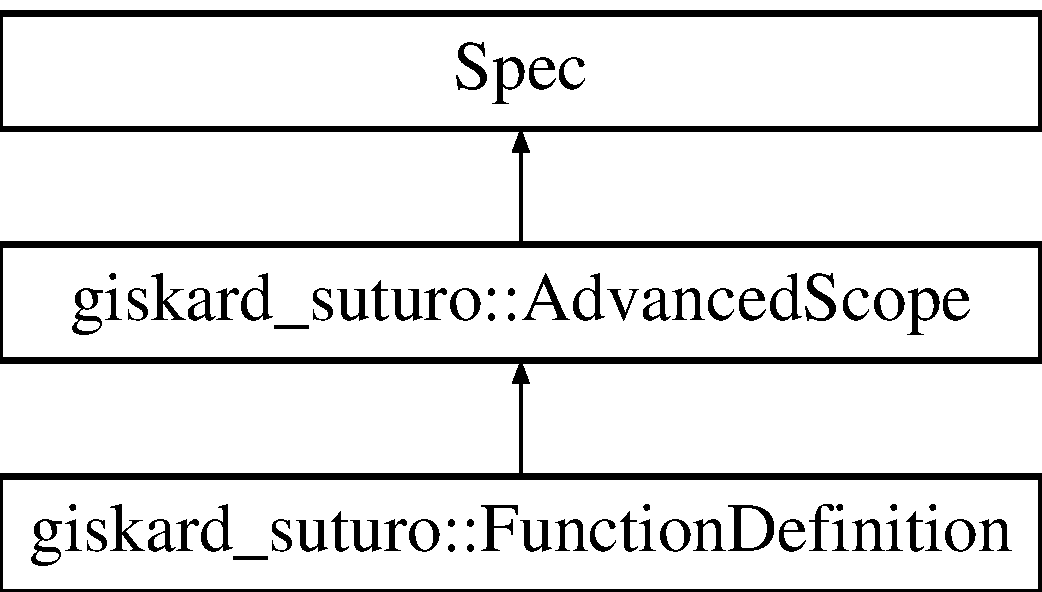
\includegraphics[height=3.000000cm]{classgiskard__suturo_1_1AdvancedScope}
\end{center}
\end{figure}
\subsection*{Classes}
\begin{DoxyCompactItemize}
\item 
struct \hyperlink{structgiskard__suturo_1_1AdvancedScope_1_1ScopeInsert}{Scope\-Insert}
\begin{DoxyCompactList}\small\item\em Structure recording under which name a scope was inserted into this scope. \end{DoxyCompactList}\end{DoxyCompactItemize}
\subsection*{Public Member Functions}
\begin{DoxyCompactItemize}
\item 
\hyperlink{classgiskard__suturo_1_1AdvancedScope_abd316ae06ac4991dbb381990546de4cd}{Advanced\-Scope} (std\-::string \-\_\-file\-Path=\char`\"{}\char`\"{}, std\-::string \-\_\-search\-Path=\char`\"{}\char`\"{}, std\-::string \-\_\-prefix=\char`\"{}\char`\"{}, std\-::vector$<$ Advanced\-Scope\-Ptr $>$ \-\_\-super\-Scopes=std\-::vector$<$ Advanced\-Scope\-Ptr $>$())
\begin{DoxyCompactList}\small\item\em Constructor for the advanced scope class. \end{DoxyCompactList}\item 
virtual void \hyperlink{classgiskard__suturo_1_1AdvancedScope_af2149977ef0016e5139f7b89f515de5b}{add\-Spec} (Scope\-Entry entry)
\begin{DoxyCompactList}\small\item\em Inserts a scope entry into this scope. \end{DoxyCompactList}\item 
virtual void \hyperlink{classgiskard__suturo_1_1AdvancedScope_ab3f65ac01f553fabc64c899dde9a4db9}{add\-Spec} (std\-::string name, Spec\-Ptr spec)
\begin{DoxyCompactList}\small\item\em Inserts an entry into this scope. \end{DoxyCompactList}\item 
virtual void \hyperlink{classgiskard__suturo_1_1AdvancedScope_a72372eceea6a63c12eb7cf278a7e55ec}{add\-Scope} (Advanced\-Scope\-Ptr super\-Scope)
\begin{DoxyCompactList}\small\item\em Adds a super scope to this scope. \end{DoxyCompactList}\item 
virtual void \hyperlink{classgiskard__suturo_1_1AdvancedScope_ad67b4f7fdf25994fccf3a553b741ecd4}{add\-Scope} (std\-::string alias, Advanced\-Scope\-Ptr super\-Scope)
\begin{DoxyCompactList}\small\item\em Adds a super scope to this scope, that can be referenced by an alias. \end{DoxyCompactList}\item 
virtual void \hyperlink{classgiskard__suturo_1_1AdvancedScope_a00d4f842341d0bda0af8e6a7fe5a1746}{add\-Function} (Fn\-Def\-Ptr function)
\begin{DoxyCompactList}\small\item\em Adds a function definition to this scope. \end{DoxyCompactList}\item 
Spec\-Ptr \hyperlink{classgiskard__suturo_1_1AdvancedScope_a5f51209c16c4267f4dea99ea66780e68}{call\-Function} (const std\-::string \&name, std\-::vector$<$ Spec\-Ptr $>$ \&arguments, Advanced\-Scope\-Ptr \&caller)
\begin{DoxyCompactList}\small\item\em Generates a function call to the named function with the given arguments. The function can be defined either in this scope or in the super scopes. \end{DoxyCompactList}\item 
Spec\-Ptr \hyperlink{classgiskard__suturo_1_1AdvancedScope_a155e1556e7180712c939cb63c7904ee4}{call\-Local\-Function} (const std\-::string \&name, std\-::vector$<$ Spec\-Ptr $>$ \&arguments, Advanced\-Scope\-Ptr \&caller)
\begin{DoxyCompactList}\small\item\em Generates a function call to the named function with the given arguments. The function must be defined in this scope. \end{DoxyCompactList}\item 
bool \hyperlink{classgiskard__suturo_1_1AdvancedScope_ab3e2735f8e0e947dbb76a6bae17f63a4}{has\-Function\-Call} (const std\-::string \&name, std\-::vector$<$ Spec\-Ptr $>$ \&arguments, \hyperlink{structgiskard__suturo_1_1FunctionCall}{Function\-Call} \&call) const 
\begin{DoxyCompactList}\small\item\em Determines whether a function has been called before with the given arguments. \end{DoxyCompactList}\item 
bool \hyperlink{classgiskard__suturo_1_1AdvancedScope_a613ef84fadf020dc111737499db7b8bb}{has\-Function} (const std\-::string \&name, const std\-::vector$<$ Spec\-Ptr $>$ \&signature) const 
\begin{DoxyCompactList}\small\item\em Determines whether this scope or one of it's super scopes defines a function with matching name and argument signature. \end{DoxyCompactList}\item 
Spec\-Ptr \hyperlink{classgiskard__suturo_1_1AdvancedScope_a6e4525139ff040d42a073643bb0ab483}{get\-Local\-Spec} (const std\-::string \&name) const 
\begin{DoxyCompactList}\small\item\em Search for a specification only in this scope. \end{DoxyCompactList}\item 
Spec\-Ptr \hyperlink{classgiskard__suturo_1_1AdvancedScope_ab44fac23fb71135abd66b65a5053a3ee}{get\-Spec} (const std\-::string \&name) const 
\begin{DoxyCompactList}\small\item\em Find a specification in this scope or it's super scopes. \end{DoxyCompactList}\item 
Spec\-Ptr \hyperlink{classgiskard__suturo_1_1AdvancedScope_a0381a9d28f74e2ce9101e65ea280e05b}{get\-Spec} (const std\-::string \&name, std\-::string \&global\-Prefix) const 
\begin{DoxyCompactList}\small\item\em Find a specification and attach the give prefix to the reference. \end{DoxyCompactList}\item 
Advanced\-Scope\-Ptr \hyperlink{classgiskard__suturo_1_1AdvancedScope_a21718dbd064b203878bea71ed38e41c0}{get\-Scope} (const std\-::string \&alias) const 
\begin{DoxyCompactList}\small\item\em Get a scope by it's alias. \end{DoxyCompactList}\item 
Advanced\-Scope\-Ptr \hyperlink{classgiskard__suturo_1_1AdvancedScope_a7489f59d843c5ae6cd0849b7bfd08579}{get\-Scope\-By\-File} (const std\-::string \&\hyperlink{classgiskard__suturo_1_1AdvancedScope_a2b3e583a28325902fec73e0063646cab}{file\-Path}) const 
\begin{DoxyCompactList}\small\item\em Get a scope by the file it was generated from. \end{DoxyCompactList}\item 
bool \hyperlink{classgiskard__suturo_1_1AdvancedScope_a96cdc688a623cf277ea441533813e16b}{is\-Super\-Scope} (const std\-::string \&\hyperlink{classgiskard__suturo_1_1AdvancedScope_a2b3e583a28325902fec73e0063646cab}{file\-Path}) const 
\begin{DoxyCompactList}\small\item\em Determines whether one of this scope's super scopes is generated from the given file. \end{DoxyCompactList}\item 
bool \hyperlink{classgiskard__suturo_1_1AdvancedScope_af1e4c6fa16b5ee78fcc58c17a8b0dfeb}{is\-Name\-Taken} (const std\-::string \&name) const 
\begin{DoxyCompactList}\small\item\em Determines whether a name is already taken. \end{DoxyCompactList}\item 
bool \hyperlink{classgiskard__suturo_1_1AdvancedScope_a5bc06fbeb129fe8955f66a468dcf4b63}{equals} (const Spec \&other) const 
\begin{DoxyCompactList}\small\item\em Equality check required by giskard\-\_\-core\-::\-Spec. \end{DoxyCompactList}\item 
void \hyperlink{classgiskard__suturo_1_1AdvancedScope_a618f025a37c10a1e5daedbe7552b29ea}{get\-\_\-input\-\_\-specs} (std\-::vector$<$ const Input\-Spec $\ast$ $>$ \&inputs) const 
\begin{DoxyCompactList}\small\item\em Gets the input specs. Required by giskard\-\_\-core\-::\-Spec. \end{DoxyCompactList}\item 
void \hyperlink{classgiskard__suturo_1_1AdvancedScope_a7fde68d72d367aeb8cdda1fff7b39fbe}{convert} (Scope\-Spec \&scope, std\-::unordered\-\_\-set$<$ const \hyperlink{classgiskard__suturo_1_1AdvancedScope}{Advanced\-Scope} $\ast$ $>$ \&generated) const 
\begin{DoxyCompactList}\small\item\em Generation method generating a giskard\-\_\-core\-::\-Scope\-Spec from this scope. \end{DoxyCompactList}\item 
std\-::vector$<$ Advanced\-Scope\-Ptr $>$ \hyperlink{classgiskard__suturo_1_1AdvancedScope_a617f245bf85101b329f02b1bbbb36adf}{get\-Super\-Scopes} () const 
\begin{DoxyCompactList}\small\item\em Get a list of all of this scope's super scopes. \end{DoxyCompactList}\item 
const std\-::string \& \hyperlink{classgiskard__suturo_1_1AdvancedScope_aaa72dd5b730fd5d97d25f9c4ed902630}{get\-Prefix} () const 
\begin{DoxyCompactList}\small\item\em Get this scope's global prefix. \end{DoxyCompactList}\end{DoxyCompactItemize}
\subsection*{Public Attributes}
\begin{DoxyCompactItemize}
\item 
const std\-::string \hyperlink{classgiskard__suturo_1_1AdvancedScope_a2b3e583a28325902fec73e0063646cab}{file\-Path}
\item 
const std\-::string \hyperlink{classgiskard__suturo_1_1AdvancedScope_a10d0cc3f9602ef2bca32dd44bc49e30e}{search\-Path}
\end{DoxyCompactItemize}
\subsection*{Static Public Attributes}
\begin{DoxyCompactItemize}
\item 
static const std\-::string \hyperlink{classgiskard__suturo_1_1AdvancedScope_a2cc175184a5c1f1e9ca8265cfb5463bc}{f\-Abs} = \char`\"{}abs\char`\"{}
\item 
\hypertarget{classgiskard__suturo_1_1AdvancedScope_a229cb23a623f37c4f3533efb0a7c26c5}{static const std\-::string {\bfseries f\-Sin} = \char`\"{}sin\char`\"{}}\label{classgiskard__suturo_1_1AdvancedScope_a229cb23a623f37c4f3533efb0a7c26c5}

\item 
\hypertarget{classgiskard__suturo_1_1AdvancedScope_ac8939a6445302c56481d5e5ab2aa2260}{static const std\-::string {\bfseries f\-Cos} = \char`\"{}cos\char`\"{}}\label{classgiskard__suturo_1_1AdvancedScope_ac8939a6445302c56481d5e5ab2aa2260}

\item 
\hypertarget{classgiskard__suturo_1_1AdvancedScope_a8e90b6ecdf4391956ce88b0328fe2d66}{static const std\-::string {\bfseries f\-Tan} = \char`\"{}tan\char`\"{}}\label{classgiskard__suturo_1_1AdvancedScope_a8e90b6ecdf4391956ce88b0328fe2d66}

\item 
\hypertarget{classgiskard__suturo_1_1AdvancedScope_a925b5ff49be8abcea970900841796087}{static const std\-::string {\bfseries f\-A\-Sin} = \char`\"{}asin\char`\"{}}\label{classgiskard__suturo_1_1AdvancedScope_a925b5ff49be8abcea970900841796087}

\item 
\hypertarget{classgiskard__suturo_1_1AdvancedScope_a55ae314601243ceca32285fc17d06943}{static const std\-::string {\bfseries f\-A\-Cos} = \char`\"{}acos\char`\"{}}\label{classgiskard__suturo_1_1AdvancedScope_a55ae314601243ceca32285fc17d06943}

\item 
\hypertarget{classgiskard__suturo_1_1AdvancedScope_ad0522497c8ce16b5ec56abf2d2c9403b}{static const std\-::string {\bfseries f\-A\-Tan} = \char`\"{}atan\char`\"{}}\label{classgiskard__suturo_1_1AdvancedScope_ad0522497c8ce16b5ec56abf2d2c9403b}

\item 
\hypertarget{classgiskard__suturo_1_1AdvancedScope_a73b18d71f520b6621e556470b7e60c1d}{static const std\-::string {\bfseries f\-F\-Mod} = \char`\"{}fmod\char`\"{}}\label{classgiskard__suturo_1_1AdvancedScope_a73b18d71f520b6621e556470b7e60c1d}

\item 
\hypertarget{classgiskard__suturo_1_1AdvancedScope_a74b316e323409569e45caa2072fe0b3a}{static const std\-::string {\bfseries f\-Max} = \char`\"{}max\char`\"{}}\label{classgiskard__suturo_1_1AdvancedScope_a74b316e323409569e45caa2072fe0b3a}

\item 
\hypertarget{classgiskard__suturo_1_1AdvancedScope_ab635fc6b4b11aef4cd62cfd05cb41101}{static const std\-::string {\bfseries f\-Min} = \char`\"{}min\char`\"{}}\label{classgiskard__suturo_1_1AdvancedScope_ab635fc6b4b11aef4cd62cfd05cb41101}

\item 
\hypertarget{classgiskard__suturo_1_1AdvancedScope_a84317a70e4f9848c605ea6146680ea56}{static const std\-::string {\bfseries f\-If} = \char`\"{}if\char`\"{}}\label{classgiskard__suturo_1_1AdvancedScope_a84317a70e4f9848c605ea6146680ea56}

\item 
\hypertarget{classgiskard__suturo_1_1AdvancedScope_a9dfbba0ef6ef69e48b4af6e14eedd320}{static const std\-::string {\bfseries f\-Norm} = \char`\"{}norm\char`\"{}}\label{classgiskard__suturo_1_1AdvancedScope_a9dfbba0ef6ef69e48b4af6e14eedd320}

\item 
\hypertarget{classgiskard__suturo_1_1AdvancedScope_a483ae8d453909b20d73f91663c2b8fac}{static const std\-::string {\bfseries f\-Slerp} = \char`\"{}slerp\char`\"{}}\label{classgiskard__suturo_1_1AdvancedScope_a483ae8d453909b20d73f91663c2b8fac}

\item 
\hypertarget{classgiskard__suturo_1_1AdvancedScope_a1569a558fda38cf17016a0acfc70528a}{static const std\-::string {\bfseries f\-Cross} = \char`\"{}cross\char`\"{}}\label{classgiskard__suturo_1_1AdvancedScope_a1569a558fda38cf17016a0acfc70528a}

\item 
\hypertarget{classgiskard__suturo_1_1AdvancedScope_a184e75e674ae425e6960f0782a0ec521}{static const std\-::string {\bfseries f\-Invert} = \char`\"{}invert\char`\"{}}\label{classgiskard__suturo_1_1AdvancedScope_a184e75e674ae425e6960f0782a0ec521}

\item 
\hypertarget{classgiskard__suturo_1_1AdvancedScope_a3c935d0795ddbd53815578743bae76ff}{static const std\-::string {\bfseries f\-In\-Scalar} = \char`\"{}input\-Scalar\char`\"{}}\label{classgiskard__suturo_1_1AdvancedScope_a3c935d0795ddbd53815578743bae76ff}

\item 
\hypertarget{classgiskard__suturo_1_1AdvancedScope_a9422f2a3ced8d5b26cbe9b8bbbd23188}{static const std\-::string {\bfseries f\-In\-Joint} = \char`\"{}input\-Joint\char`\"{}}\label{classgiskard__suturo_1_1AdvancedScope_a9422f2a3ced8d5b26cbe9b8bbbd23188}

\item 
\hypertarget{classgiskard__suturo_1_1AdvancedScope_ab402ad810b3f7fca305851fab396cb16}{static const std\-::string {\bfseries f\-In\-Vec3} = \char`\"{}input\-Vec3\char`\"{}}\label{classgiskard__suturo_1_1AdvancedScope_ab402ad810b3f7fca305851fab396cb16}

\item 
\hypertarget{classgiskard__suturo_1_1AdvancedScope_adde25528eee6dc5a1c61a36a5e713d76}{static const std\-::string {\bfseries f\-In\-Rotation} = \char`\"{}input\-Rotation\char`\"{}}\label{classgiskard__suturo_1_1AdvancedScope_adde25528eee6dc5a1c61a36a5e713d76}

\item 
\hypertarget{classgiskard__suturo_1_1AdvancedScope_a66d281a35eb22330caaaac0ca9d1e4d8}{static const std\-::string {\bfseries f\-In\-Frame} = \char`\"{}input\-Frame\char`\"{}}\label{classgiskard__suturo_1_1AdvancedScope_a66d281a35eb22330caaaac0ca9d1e4d8}

\item 
\hypertarget{classgiskard__suturo_1_1AdvancedScope_ad5bb37db8e30289c3c35b8745e00912a}{static const std\-::string {\bfseries f\-C\-Vec3} = Giskard\-P\-P\-Parser\-::s\-Vec3}\label{classgiskard__suturo_1_1AdvancedScope_ad5bb37db8e30289c3c35b8745e00912a}

\item 
\hypertarget{classgiskard__suturo_1_1AdvancedScope_a47a64840e1430d0a7268eac235b2b32d}{static const std\-::string {\bfseries f\-C\-Rotation} = Giskard\-P\-P\-Parser\-::s\-Rotation}\label{classgiskard__suturo_1_1AdvancedScope_a47a64840e1430d0a7268eac235b2b32d}

\item 
\hypertarget{classgiskard__suturo_1_1AdvancedScope_a9b4dd4bb9124f90e49adfaaf1b8b5ba5}{static const std\-::string {\bfseries f\-C\-Frame} = Giskard\-P\-P\-Parser\-::s\-Frame}\label{classgiskard__suturo_1_1AdvancedScope_a9b4dd4bb9124f90e49adfaaf1b8b5ba5}

\item 
\hypertarget{classgiskard__suturo_1_1AdvancedScope_ae2d7c13d5e7940be15a9dfd9c0f0dda1}{static const std\-::string {\bfseries f\-C\-Hard\-C} = Giskard\-P\-P\-Parser\-::s\-Hard}\label{classgiskard__suturo_1_1AdvancedScope_ae2d7c13d5e7940be15a9dfd9c0f0dda1}

\item 
\hypertarget{classgiskard__suturo_1_1AdvancedScope_aff09a5d9175eb5ecd2e623eea81cb574}{static const std\-::string {\bfseries f\-C\-Soft\-C} = Giskard\-P\-P\-Parser\-::s\-Soft}\label{classgiskard__suturo_1_1AdvancedScope_aff09a5d9175eb5ecd2e623eea81cb574}

\item 
\hypertarget{classgiskard__suturo_1_1AdvancedScope_acd3551f4badb7c595a2c37739b09d12c}{static const std\-::string {\bfseries f\-C\-Cont\-C} = Giskard\-P\-P\-Parser\-::s\-Controllable}\label{classgiskard__suturo_1_1AdvancedScope_acd3551f4badb7c595a2c37739b09d12c}

\end{DoxyCompactItemize}
\subsection*{Protected Attributes}
\begin{DoxyCompactItemize}
\item 
std\-::string \hyperlink{classgiskard__suturo_1_1AdvancedScope_ac69aab3b5b22fc62d1d0f8e213e86ec5}{prefix}
\item 
std\-::vector$<$ std\-::string $>$ \hyperlink{classgiskard__suturo_1_1AdvancedScope_a6a788662a6c7df9eaa3a8419b466990d}{spec\-Insert\-History}
\item 
std\-::vector$<$ \hyperlink{structgiskard__suturo_1_1AdvancedScope_1_1ScopeInsert}{Scope\-Insert} $>$ \hyperlink{classgiskard__suturo_1_1AdvancedScope_af5081ec45e81c905ed286da7a72532c3}{scope\-Insert\-History}
\end{DoxyCompactItemize}
\subsection*{Private Attributes}
\begin{DoxyCompactItemize}
\item 
std\-::vector$<$ Advanced\-Scope\-Ptr $>$ \hyperlink{classgiskard__suturo_1_1AdvancedScope_ab4a2ea0c6a7d6401c7e5b2795a3094bb}{super\-Scopes}
\item 
std\-::unordered\-\_\-map\\*
$<$ std\-::string, \\*
Advanced\-Scope\-Ptr $>$ \hyperlink{classgiskard__suturo_1_1AdvancedScope_a9a27c5f444714caf79ec05ac606c84a5}{aliased\-Scopes}
\item 
std\-::unordered\-\_\-map\\*
$<$ std\-::string, std\-::vector\\*
$<$ Fn\-Def\-Ptr $>$ $>$ \hyperlink{classgiskard__suturo_1_1AdvancedScope_a32385ec7d5bdd31f190473293e3445f8}{function\-Definitions}
\item 
std\-::unordered\-\_\-map\\*
$<$ std\-::string, std\-::vector\\*
$<$ \hyperlink{structgiskard__suturo_1_1FunctionCall}{Function\-Call} $>$ $>$ \hyperlink{classgiskard__suturo_1_1AdvancedScope_a6208063287509649126390c5960abfb8}{function\-Calls}
\item 
std\-::unordered\-\_\-map\\*
$<$ std\-::string, Spec\-Ptr $>$ \hyperlink{classgiskard__suturo_1_1AdvancedScope_a92bbb9dc2613a1331a95f7e0310dd342}{specs}
\end{DoxyCompactItemize}


\subsection{Detailed Description}
The advanced scope class supports layered scopes and named search scopes. 

This class was specifically designed for the G\-Lang++ parser procedure. It supports concepts like super scopes that it searches when queried for an expression. It also supports aliased imported scopes that can specifically queried for expressions. 

\subsection{Constructor \& Destructor Documentation}
\hypertarget{classgiskard__suturo_1_1AdvancedScope_abd316ae06ac4991dbb381990546de4cd}{\index{giskard\-\_\-suturo\-::\-Advanced\-Scope@{giskard\-\_\-suturo\-::\-Advanced\-Scope}!Advanced\-Scope@{Advanced\-Scope}}
\index{Advanced\-Scope@{Advanced\-Scope}!giskard_suturo::AdvancedScope@{giskard\-\_\-suturo\-::\-Advanced\-Scope}}
\subsubsection[{Advanced\-Scope}]{\setlength{\rightskip}{0pt plus 5cm}giskard\-\_\-suturo\-::\-Advanced\-Scope\-::\-Advanced\-Scope (
\begin{DoxyParamCaption}
\item[{std\-::string}]{\-\_\-file\-Path = {\ttfamily \char`\"{}\char`\"{}}, }
\item[{std\-::string}]{\-\_\-search\-Path = {\ttfamily \char`\"{}\char`\"{}}, }
\item[{std\-::string}]{\-\_\-prefix = {\ttfamily \char`\"{}\char`\"{}}, }
\item[{std\-::vector$<$ Advanced\-Scope\-Ptr $>$}]{\-\_\-super\-Scopes = {\ttfamily std\-:\-:vector$<$AdvancedScopePtr$>$()}}
\end{DoxyParamCaption}
)\hspace{0.3cm}{\ttfamily [inline]}}}\label{classgiskard__suturo_1_1AdvancedScope_abd316ae06ac4991dbb381990546de4cd}


Constructor for the advanced scope class. 


\begin{DoxyParams}[1]{Parameters}
\mbox{\tt in}  & {\em \-\_\-file\-Path} & File that this scope is being parsed from \\
\hline
\mbox{\tt in}  & {\em \-\_\-search\-Path} & Base path for the relative search for imported files. \\
\hline
\mbox{\tt in}  & {\em \-\_\-prefix} & Prefix of this scope. \\
\hline
\mbox{\tt in}  & {\em \-\_\-super\-Scopes} & List of super scopes \\
\hline
\end{DoxyParams}


\subsection{Member Function Documentation}
\hypertarget{classgiskard__suturo_1_1AdvancedScope_a00d4f842341d0bda0af8e6a7fe5a1746}{\index{giskard\-\_\-suturo\-::\-Advanced\-Scope@{giskard\-\_\-suturo\-::\-Advanced\-Scope}!add\-Function@{add\-Function}}
\index{add\-Function@{add\-Function}!giskard_suturo::AdvancedScope@{giskard\-\_\-suturo\-::\-Advanced\-Scope}}
\subsubsection[{add\-Function}]{\setlength{\rightskip}{0pt plus 5cm}void giskard\-\_\-suturo\-::\-Advanced\-Scope\-::add\-Function (
\begin{DoxyParamCaption}
\item[{Fn\-Def\-Ptr}]{function}
\end{DoxyParamCaption}
)\hspace{0.3cm}{\ttfamily [virtual]}}}\label{classgiskard__suturo_1_1AdvancedScope_a00d4f842341d0bda0af8e6a7fe5a1746}


Adds a function definition to this scope. 


\begin{DoxyParams}[1]{Parameters}
\mbox{\tt in}  & {\em function} & The function definition to add \\
\hline
\end{DoxyParams}
\hypertarget{classgiskard__suturo_1_1AdvancedScope_a72372eceea6a63c12eb7cf278a7e55ec}{\index{giskard\-\_\-suturo\-::\-Advanced\-Scope@{giskard\-\_\-suturo\-::\-Advanced\-Scope}!add\-Scope@{add\-Scope}}
\index{add\-Scope@{add\-Scope}!giskard_suturo::AdvancedScope@{giskard\-\_\-suturo\-::\-Advanced\-Scope}}
\subsubsection[{add\-Scope}]{\setlength{\rightskip}{0pt plus 5cm}void giskard\-\_\-suturo\-::\-Advanced\-Scope\-::add\-Scope (
\begin{DoxyParamCaption}
\item[{Advanced\-Scope\-Ptr}]{super\-Scope}
\end{DoxyParamCaption}
)\hspace{0.3cm}{\ttfamily [virtual]}}}\label{classgiskard__suturo_1_1AdvancedScope_a72372eceea6a63c12eb7cf278a7e55ec}


Adds a super scope to this scope. 


\begin{DoxyParams}[1]{Parameters}
\mbox{\tt in}  & {\em super\-Scope} & The super scope \\
\hline
\end{DoxyParams}
\hypertarget{classgiskard__suturo_1_1AdvancedScope_ad67b4f7fdf25994fccf3a553b741ecd4}{\index{giskard\-\_\-suturo\-::\-Advanced\-Scope@{giskard\-\_\-suturo\-::\-Advanced\-Scope}!add\-Scope@{add\-Scope}}
\index{add\-Scope@{add\-Scope}!giskard_suturo::AdvancedScope@{giskard\-\_\-suturo\-::\-Advanced\-Scope}}
\subsubsection[{add\-Scope}]{\setlength{\rightskip}{0pt plus 5cm}void giskard\-\_\-suturo\-::\-Advanced\-Scope\-::add\-Scope (
\begin{DoxyParamCaption}
\item[{std\-::string}]{alias, }
\item[{Advanced\-Scope\-Ptr}]{super\-Scope}
\end{DoxyParamCaption}
)\hspace{0.3cm}{\ttfamily [virtual]}}}\label{classgiskard__suturo_1_1AdvancedScope_ad67b4f7fdf25994fccf3a553b741ecd4}


Adds a super scope to this scope, that can be referenced by an alias. 


\begin{DoxyParams}[1]{Parameters}
\mbox{\tt in}  & {\em alias} & Alias to use for this scope \\
\hline
\mbox{\tt in}  & {\em super\-Scope} & Scope to add \\
\hline
\end{DoxyParams}
\hypertarget{classgiskard__suturo_1_1AdvancedScope_af2149977ef0016e5139f7b89f515de5b}{\index{giskard\-\_\-suturo\-::\-Advanced\-Scope@{giskard\-\_\-suturo\-::\-Advanced\-Scope}!add\-Spec@{add\-Spec}}
\index{add\-Spec@{add\-Spec}!giskard_suturo::AdvancedScope@{giskard\-\_\-suturo\-::\-Advanced\-Scope}}
\subsubsection[{add\-Spec}]{\setlength{\rightskip}{0pt plus 5cm}void giskard\-\_\-suturo\-::\-Advanced\-Scope\-::add\-Spec (
\begin{DoxyParamCaption}
\item[{Scope\-Entry}]{entry}
\end{DoxyParamCaption}
)\hspace{0.3cm}{\ttfamily [virtual]}}}\label{classgiskard__suturo_1_1AdvancedScope_af2149977ef0016e5139f7b89f515de5b}


Inserts a scope entry into this scope. 


\begin{DoxyParams}[1]{Parameters}
\mbox{\tt in}  & {\em entry} & The entry to insert \\
\hline
\end{DoxyParams}
\hypertarget{classgiskard__suturo_1_1AdvancedScope_ab3f65ac01f553fabc64c899dde9a4db9}{\index{giskard\-\_\-suturo\-::\-Advanced\-Scope@{giskard\-\_\-suturo\-::\-Advanced\-Scope}!add\-Spec@{add\-Spec}}
\index{add\-Spec@{add\-Spec}!giskard_suturo::AdvancedScope@{giskard\-\_\-suturo\-::\-Advanced\-Scope}}
\subsubsection[{add\-Spec}]{\setlength{\rightskip}{0pt plus 5cm}void giskard\-\_\-suturo\-::\-Advanced\-Scope\-::add\-Spec (
\begin{DoxyParamCaption}
\item[{std\-::string}]{name, }
\item[{Spec\-Ptr}]{spec}
\end{DoxyParamCaption}
)\hspace{0.3cm}{\ttfamily [virtual]}}}\label{classgiskard__suturo_1_1AdvancedScope_ab3f65ac01f553fabc64c899dde9a4db9}


Inserts an entry into this scope. 


\begin{DoxyParams}[1]{Parameters}
\mbox{\tt in}  & {\em name} & Name of the entry \\
\hline
\mbox{\tt in}  & {\em spec} & Specification of the expression \\
\hline
\end{DoxyParams}


Reimplemented in \hyperlink{classgiskard__suturo_1_1FunctionDefinition_a723dc9bc2d5f964805dadc8af9a8c948}{giskard\-\_\-suturo\-::\-Function\-Definition}.

\hypertarget{classgiskard__suturo_1_1AdvancedScope_a5f51209c16c4267f4dea99ea66780e68}{\index{giskard\-\_\-suturo\-::\-Advanced\-Scope@{giskard\-\_\-suturo\-::\-Advanced\-Scope}!call\-Function@{call\-Function}}
\index{call\-Function@{call\-Function}!giskard_suturo::AdvancedScope@{giskard\-\_\-suturo\-::\-Advanced\-Scope}}
\subsubsection[{call\-Function}]{\setlength{\rightskip}{0pt plus 5cm}Spec\-Ptr giskard\-\_\-suturo\-::\-Advanced\-Scope\-::call\-Function (
\begin{DoxyParamCaption}
\item[{const std\-::string \&}]{name, }
\item[{std\-::vector$<$ Spec\-Ptr $>$ \&}]{arguments, }
\item[{Advanced\-Scope\-Ptr \&}]{caller}
\end{DoxyParamCaption}
)}}\label{classgiskard__suturo_1_1AdvancedScope_a5f51209c16c4267f4dea99ea66780e68}


Generates a function call to the named function with the given arguments. The function can be defined either in this scope or in the super scopes. 


\begin{DoxyParams}[1]{Parameters}
\mbox{\tt in}  & {\em name} & Name of the function \\
\hline
 & {\em arguments} & Arguments for the call \\
\hline
 & {\em caller} & The scope that is calling the function\\
\hline
\end{DoxyParams}
\begin{DoxyReturn}{Returns}
The generated specification 
\end{DoxyReturn}
\hypertarget{classgiskard__suturo_1_1AdvancedScope_a155e1556e7180712c939cb63c7904ee4}{\index{giskard\-\_\-suturo\-::\-Advanced\-Scope@{giskard\-\_\-suturo\-::\-Advanced\-Scope}!call\-Local\-Function@{call\-Local\-Function}}
\index{call\-Local\-Function@{call\-Local\-Function}!giskard_suturo::AdvancedScope@{giskard\-\_\-suturo\-::\-Advanced\-Scope}}
\subsubsection[{call\-Local\-Function}]{\setlength{\rightskip}{0pt plus 5cm}Spec\-Ptr giskard\-\_\-suturo\-::\-Advanced\-Scope\-::call\-Local\-Function (
\begin{DoxyParamCaption}
\item[{const std\-::string \&}]{name, }
\item[{std\-::vector$<$ Spec\-Ptr $>$ \&}]{arguments, }
\item[{Advanced\-Scope\-Ptr \&}]{caller}
\end{DoxyParamCaption}
)}}\label{classgiskard__suturo_1_1AdvancedScope_a155e1556e7180712c939cb63c7904ee4}


Generates a function call to the named function with the given arguments. The function must be defined in this scope. 


\begin{DoxyParams}[1]{Parameters}
\mbox{\tt in}  & {\em name} & Name of the function \\
\hline
 & {\em arguments} & Arguments for the call \\
\hline
 & {\em caller} & The scope making the call\\
\hline
\end{DoxyParams}
\begin{DoxyReturn}{Returns}
\{ description\-\_\-of\-\_\-the\-\_\-return\-\_\-value \} 
\end{DoxyReturn}
\hypertarget{classgiskard__suturo_1_1AdvancedScope_a7fde68d72d367aeb8cdda1fff7b39fbe}{\index{giskard\-\_\-suturo\-::\-Advanced\-Scope@{giskard\-\_\-suturo\-::\-Advanced\-Scope}!convert@{convert}}
\index{convert@{convert}!giskard_suturo::AdvancedScope@{giskard\-\_\-suturo\-::\-Advanced\-Scope}}
\subsubsection[{convert}]{\setlength{\rightskip}{0pt plus 5cm}void giskard\-\_\-suturo\-::\-Advanced\-Scope\-::convert (
\begin{DoxyParamCaption}
\item[{Scope\-Spec \&}]{scope, }
\item[{std\-::unordered\-\_\-set$<$ const {\bf Advanced\-Scope} $\ast$ $>$ \&}]{generated}
\end{DoxyParamCaption}
) const}}\label{classgiskard__suturo_1_1AdvancedScope_a7fde68d72d367aeb8cdda1fff7b39fbe}


Generation method generating a giskard\-\_\-core\-::\-Scope\-Spec from this scope. 


\begin{DoxyParams}{Parameters}
{\em scope} & Scope being generated \\
\hline
{\em generated} & Scopes that were already generated \\
\hline
\end{DoxyParams}
\hypertarget{classgiskard__suturo_1_1AdvancedScope_a5bc06fbeb129fe8955f66a468dcf4b63}{\index{giskard\-\_\-suturo\-::\-Advanced\-Scope@{giskard\-\_\-suturo\-::\-Advanced\-Scope}!equals@{equals}}
\index{equals@{equals}!giskard_suturo::AdvancedScope@{giskard\-\_\-suturo\-::\-Advanced\-Scope}}
\subsubsection[{equals}]{\setlength{\rightskip}{0pt plus 5cm}bool giskard\-\_\-suturo\-::\-Advanced\-Scope\-::equals (
\begin{DoxyParamCaption}
\item[{const Spec \&}]{other}
\end{DoxyParamCaption}
) const}}\label{classgiskard__suturo_1_1AdvancedScope_a5bc06fbeb129fe8955f66a468dcf4b63}


Equality check required by giskard\-\_\-core\-::\-Spec. 


\begin{DoxyParams}[1]{Parameters}
\mbox{\tt in}  & {\em other} & The other specification\\
\hline
\end{DoxyParams}
\begin{DoxyReturn}{Returns}
True if scope equals other specification 
\end{DoxyReturn}
\hypertarget{classgiskard__suturo_1_1AdvancedScope_a618f025a37c10a1e5daedbe7552b29ea}{\index{giskard\-\_\-suturo\-::\-Advanced\-Scope@{giskard\-\_\-suturo\-::\-Advanced\-Scope}!get\-\_\-input\-\_\-specs@{get\-\_\-input\-\_\-specs}}
\index{get\-\_\-input\-\_\-specs@{get\-\_\-input\-\_\-specs}!giskard_suturo::AdvancedScope@{giskard\-\_\-suturo\-::\-Advanced\-Scope}}
\subsubsection[{get\-\_\-input\-\_\-specs}]{\setlength{\rightskip}{0pt plus 5cm}void giskard\-\_\-suturo\-::\-Advanced\-Scope\-::get\-\_\-input\-\_\-specs (
\begin{DoxyParamCaption}
\item[{std\-::vector$<$ const Input\-Spec $\ast$ $>$ \&}]{inputs}
\end{DoxyParamCaption}
) const\hspace{0.3cm}{\ttfamily [inline]}}}\label{classgiskard__suturo_1_1AdvancedScope_a618f025a37c10a1e5daedbe7552b29ea}


Gets the input specs. Required by giskard\-\_\-core\-::\-Spec. 


\begin{DoxyParams}{Parameters}
{\em inputs} & List of found inputs \\
\hline
\end{DoxyParams}
\hypertarget{classgiskard__suturo_1_1AdvancedScope_a6e4525139ff040d42a073643bb0ab483}{\index{giskard\-\_\-suturo\-::\-Advanced\-Scope@{giskard\-\_\-suturo\-::\-Advanced\-Scope}!get\-Local\-Spec@{get\-Local\-Spec}}
\index{get\-Local\-Spec@{get\-Local\-Spec}!giskard_suturo::AdvancedScope@{giskard\-\_\-suturo\-::\-Advanced\-Scope}}
\subsubsection[{get\-Local\-Spec}]{\setlength{\rightskip}{0pt plus 5cm}Spec\-Ptr giskard\-\_\-suturo\-::\-Advanced\-Scope\-::get\-Local\-Spec (
\begin{DoxyParamCaption}
\item[{const std\-::string \&}]{name}
\end{DoxyParamCaption}
) const}}\label{classgiskard__suturo_1_1AdvancedScope_a6e4525139ff040d42a073643bb0ab483}


Search for a specification only in this scope. 


\begin{DoxyParams}[1]{Parameters}
\mbox{\tt in}  & {\em name} & Name of the specification\\
\hline
\end{DoxyParams}
\begin{DoxyReturn}{Returns}
Found specification 
\end{DoxyReturn}
\hypertarget{classgiskard__suturo_1_1AdvancedScope_aaa72dd5b730fd5d97d25f9c4ed902630}{\index{giskard\-\_\-suturo\-::\-Advanced\-Scope@{giskard\-\_\-suturo\-::\-Advanced\-Scope}!get\-Prefix@{get\-Prefix}}
\index{get\-Prefix@{get\-Prefix}!giskard_suturo::AdvancedScope@{giskard\-\_\-suturo\-::\-Advanced\-Scope}}
\subsubsection[{get\-Prefix}]{\setlength{\rightskip}{0pt plus 5cm}const std\-::string\& giskard\-\_\-suturo\-::\-Advanced\-Scope\-::get\-Prefix (
\begin{DoxyParamCaption}
{}
\end{DoxyParamCaption}
) const\hspace{0.3cm}{\ttfamily [inline]}}}\label{classgiskard__suturo_1_1AdvancedScope_aaa72dd5b730fd5d97d25f9c4ed902630}


Get this scope's global prefix. 

\begin{DoxyReturn}{Returns}
Prefix. 
\end{DoxyReturn}
\hypertarget{classgiskard__suturo_1_1AdvancedScope_a21718dbd064b203878bea71ed38e41c0}{\index{giskard\-\_\-suturo\-::\-Advanced\-Scope@{giskard\-\_\-suturo\-::\-Advanced\-Scope}!get\-Scope@{get\-Scope}}
\index{get\-Scope@{get\-Scope}!giskard_suturo::AdvancedScope@{giskard\-\_\-suturo\-::\-Advanced\-Scope}}
\subsubsection[{get\-Scope}]{\setlength{\rightskip}{0pt plus 5cm}Advanced\-Scope\-Ptr giskard\-\_\-suturo\-::\-Advanced\-Scope\-::get\-Scope (
\begin{DoxyParamCaption}
\item[{const std\-::string \&}]{alias}
\end{DoxyParamCaption}
) const}}\label{classgiskard__suturo_1_1AdvancedScope_a21718dbd064b203878bea71ed38e41c0}


Get a scope by it's alias. 


\begin{DoxyParams}[1]{Parameters}
\mbox{\tt in}  & {\em alias} & Alias of the scope\\
\hline
\end{DoxyParams}
\begin{DoxyReturn}{Returns}
Pointer to the scope 
\end{DoxyReturn}
\hypertarget{classgiskard__suturo_1_1AdvancedScope_a7489f59d843c5ae6cd0849b7bfd08579}{\index{giskard\-\_\-suturo\-::\-Advanced\-Scope@{giskard\-\_\-suturo\-::\-Advanced\-Scope}!get\-Scope\-By\-File@{get\-Scope\-By\-File}}
\index{get\-Scope\-By\-File@{get\-Scope\-By\-File}!giskard_suturo::AdvancedScope@{giskard\-\_\-suturo\-::\-Advanced\-Scope}}
\subsubsection[{get\-Scope\-By\-File}]{\setlength{\rightskip}{0pt plus 5cm}Advanced\-Scope\-Ptr giskard\-\_\-suturo\-::\-Advanced\-Scope\-::get\-Scope\-By\-File (
\begin{DoxyParamCaption}
\item[{const std\-::string \&}]{file\-Path}
\end{DoxyParamCaption}
) const}}\label{classgiskard__suturo_1_1AdvancedScope_a7489f59d843c5ae6cd0849b7bfd08579}


Get a scope by the file it was generated from. 


\begin{DoxyParams}[1]{Parameters}
\mbox{\tt in}  & {\em file\-Path} & File path\\
\hline
\end{DoxyParams}
\begin{DoxyReturn}{Returns}
Pointer to the scope 
\end{DoxyReturn}
\hypertarget{classgiskard__suturo_1_1AdvancedScope_ab44fac23fb71135abd66b65a5053a3ee}{\index{giskard\-\_\-suturo\-::\-Advanced\-Scope@{giskard\-\_\-suturo\-::\-Advanced\-Scope}!get\-Spec@{get\-Spec}}
\index{get\-Spec@{get\-Spec}!giskard_suturo::AdvancedScope@{giskard\-\_\-suturo\-::\-Advanced\-Scope}}
\subsubsection[{get\-Spec}]{\setlength{\rightskip}{0pt plus 5cm}Spec\-Ptr giskard\-\_\-suturo\-::\-Advanced\-Scope\-::get\-Spec (
\begin{DoxyParamCaption}
\item[{const std\-::string \&}]{name}
\end{DoxyParamCaption}
) const}}\label{classgiskard__suturo_1_1AdvancedScope_ab44fac23fb71135abd66b65a5053a3ee}


Find a specification in this scope or it's super scopes. 


\begin{DoxyParams}[1]{Parameters}
\mbox{\tt in}  & {\em name} & Name of the specification\\
\hline
\end{DoxyParams}
\begin{DoxyReturn}{Returns}
Found specification 
\end{DoxyReturn}
\hypertarget{classgiskard__suturo_1_1AdvancedScope_a0381a9d28f74e2ce9101e65ea280e05b}{\index{giskard\-\_\-suturo\-::\-Advanced\-Scope@{giskard\-\_\-suturo\-::\-Advanced\-Scope}!get\-Spec@{get\-Spec}}
\index{get\-Spec@{get\-Spec}!giskard_suturo::AdvancedScope@{giskard\-\_\-suturo\-::\-Advanced\-Scope}}
\subsubsection[{get\-Spec}]{\setlength{\rightskip}{0pt plus 5cm}Spec\-Ptr giskard\-\_\-suturo\-::\-Advanced\-Scope\-::get\-Spec (
\begin{DoxyParamCaption}
\item[{const std\-::string \&}]{name, }
\item[{std\-::string \&}]{global\-Prefix}
\end{DoxyParamCaption}
) const}}\label{classgiskard__suturo_1_1AdvancedScope_a0381a9d28f74e2ce9101e65ea280e05b}


Find a specification and attach the give prefix to the reference. 


\begin{DoxyParams}[1]{Parameters}
\mbox{\tt in}  & {\em name} & Name of the specification \\
\hline
 & {\em global\-Prefix} & Prefix for the reference\\
\hline
\end{DoxyParams}
\begin{DoxyReturn}{Returns}
Reference specification 
\end{DoxyReturn}
\hypertarget{classgiskard__suturo_1_1AdvancedScope_a617f245bf85101b329f02b1bbbb36adf}{\index{giskard\-\_\-suturo\-::\-Advanced\-Scope@{giskard\-\_\-suturo\-::\-Advanced\-Scope}!get\-Super\-Scopes@{get\-Super\-Scopes}}
\index{get\-Super\-Scopes@{get\-Super\-Scopes}!giskard_suturo::AdvancedScope@{giskard\-\_\-suturo\-::\-Advanced\-Scope}}
\subsubsection[{get\-Super\-Scopes}]{\setlength{\rightskip}{0pt plus 5cm}std\-::vector$<$Advanced\-Scope\-Ptr$>$ giskard\-\_\-suturo\-::\-Advanced\-Scope\-::get\-Super\-Scopes (
\begin{DoxyParamCaption}
{}
\end{DoxyParamCaption}
) const\hspace{0.3cm}{\ttfamily [inline]}}}\label{classgiskard__suturo_1_1AdvancedScope_a617f245bf85101b329f02b1bbbb36adf}


Get a list of all of this scope's super scopes. 

\begin{DoxyReturn}{Returns}
The super scopes. 
\end{DoxyReturn}
\hypertarget{classgiskard__suturo_1_1AdvancedScope_a613ef84fadf020dc111737499db7b8bb}{\index{giskard\-\_\-suturo\-::\-Advanced\-Scope@{giskard\-\_\-suturo\-::\-Advanced\-Scope}!has\-Function@{has\-Function}}
\index{has\-Function@{has\-Function}!giskard_suturo::AdvancedScope@{giskard\-\_\-suturo\-::\-Advanced\-Scope}}
\subsubsection[{has\-Function}]{\setlength{\rightskip}{0pt plus 5cm}bool giskard\-\_\-suturo\-::\-Advanced\-Scope\-::has\-Function (
\begin{DoxyParamCaption}
\item[{const std\-::string \&}]{name, }
\item[{const std\-::vector$<$ Spec\-Ptr $>$ \&}]{signature}
\end{DoxyParamCaption}
) const}}\label{classgiskard__suturo_1_1AdvancedScope_a613ef84fadf020dc111737499db7b8bb}


Determines whether this scope or one of it's super scopes defines a function with matching name and argument signature. 


\begin{DoxyParams}[1]{Parameters}
\mbox{\tt in}  & {\em name} & Name of the function \\
\hline
\mbox{\tt in}  & {\em signature} & Argument signature\\
\hline
\end{DoxyParams}
\begin{DoxyReturn}{Returns}
True if a matching function is defined 
\end{DoxyReturn}
\hypertarget{classgiskard__suturo_1_1AdvancedScope_ab3e2735f8e0e947dbb76a6bae17f63a4}{\index{giskard\-\_\-suturo\-::\-Advanced\-Scope@{giskard\-\_\-suturo\-::\-Advanced\-Scope}!has\-Function\-Call@{has\-Function\-Call}}
\index{has\-Function\-Call@{has\-Function\-Call}!giskard_suturo::AdvancedScope@{giskard\-\_\-suturo\-::\-Advanced\-Scope}}
\subsubsection[{has\-Function\-Call}]{\setlength{\rightskip}{0pt plus 5cm}bool giskard\-\_\-suturo\-::\-Advanced\-Scope\-::has\-Function\-Call (
\begin{DoxyParamCaption}
\item[{const std\-::string \&}]{name, }
\item[{std\-::vector$<$ Spec\-Ptr $>$ \&}]{arguments, }
\item[{{\bf Function\-Call} \&}]{call}
\end{DoxyParamCaption}
) const}}\label{classgiskard__suturo_1_1AdvancedScope_ab3e2735f8e0e947dbb76a6bae17f63a4}


Determines whether a function has been called before with the given arguments. 


\begin{DoxyParams}[1]{Parameters}
\mbox{\tt in}  & {\em name} & Name of the function \\
\hline
 & {\em arguments} & Arguments for the call \\
\hline
 & {\em call} & The call structure storing this call\\
\hline
\end{DoxyParams}
\begin{DoxyReturn}{Returns}
True if this function has been called with these arguments before, False otherwise. 
\end{DoxyReturn}
\hypertarget{classgiskard__suturo_1_1AdvancedScope_af1e4c6fa16b5ee78fcc58c17a8b0dfeb}{\index{giskard\-\_\-suturo\-::\-Advanced\-Scope@{giskard\-\_\-suturo\-::\-Advanced\-Scope}!is\-Name\-Taken@{is\-Name\-Taken}}
\index{is\-Name\-Taken@{is\-Name\-Taken}!giskard_suturo::AdvancedScope@{giskard\-\_\-suturo\-::\-Advanced\-Scope}}
\subsubsection[{is\-Name\-Taken}]{\setlength{\rightskip}{0pt plus 5cm}bool giskard\-\_\-suturo\-::\-Advanced\-Scope\-::is\-Name\-Taken (
\begin{DoxyParamCaption}
\item[{const std\-::string \&}]{name}
\end{DoxyParamCaption}
) const}}\label{classgiskard__suturo_1_1AdvancedScope_af1e4c6fa16b5ee78fcc58c17a8b0dfeb}


Determines whether a name is already taken. 


\begin{DoxyParams}[1]{Parameters}
\mbox{\tt in}  & {\em name} & Name to check\\
\hline
\end{DoxyParams}
\begin{DoxyReturn}{Returns}
True if the name is taken. 
\end{DoxyReturn}
\hypertarget{classgiskard__suturo_1_1AdvancedScope_a96cdc688a623cf277ea441533813e16b}{\index{giskard\-\_\-suturo\-::\-Advanced\-Scope@{giskard\-\_\-suturo\-::\-Advanced\-Scope}!is\-Super\-Scope@{is\-Super\-Scope}}
\index{is\-Super\-Scope@{is\-Super\-Scope}!giskard_suturo::AdvancedScope@{giskard\-\_\-suturo\-::\-Advanced\-Scope}}
\subsubsection[{is\-Super\-Scope}]{\setlength{\rightskip}{0pt plus 5cm}bool giskard\-\_\-suturo\-::\-Advanced\-Scope\-::is\-Super\-Scope (
\begin{DoxyParamCaption}
\item[{const std\-::string \&}]{file\-Path}
\end{DoxyParamCaption}
) const}}\label{classgiskard__suturo_1_1AdvancedScope_a96cdc688a623cf277ea441533813e16b}


Determines whether one of this scope's super scopes is generated from the given file. 


\begin{DoxyParams}[1]{Parameters}
\mbox{\tt in}  & {\em file\-Path} & File path\\
\hline
\end{DoxyParams}
\begin{DoxyReturn}{Returns}
True if a super scope is generated by this file. 
\end{DoxyReturn}


\subsection{Member Data Documentation}
\hypertarget{classgiskard__suturo_1_1AdvancedScope_a9a27c5f444714caf79ec05ac606c84a5}{\index{giskard\-\_\-suturo\-::\-Advanced\-Scope@{giskard\-\_\-suturo\-::\-Advanced\-Scope}!aliased\-Scopes@{aliased\-Scopes}}
\index{aliased\-Scopes@{aliased\-Scopes}!giskard_suturo::AdvancedScope@{giskard\-\_\-suturo\-::\-Advanced\-Scope}}
\subsubsection[{aliased\-Scopes}]{\setlength{\rightskip}{0pt plus 5cm}std\-::unordered\-\_\-map$<$std\-::string, Advanced\-Scope\-Ptr$>$ giskard\-\_\-suturo\-::\-Advanced\-Scope\-::aliased\-Scopes\hspace{0.3cm}{\ttfamily [private]}}}\label{classgiskard__suturo_1_1AdvancedScope_a9a27c5f444714caf79ec05ac606c84a5}
Aliased scopes \hypertarget{classgiskard__suturo_1_1AdvancedScope_a2cc175184a5c1f1e9ca8265cfb5463bc}{\index{giskard\-\_\-suturo\-::\-Advanced\-Scope@{giskard\-\_\-suturo\-::\-Advanced\-Scope}!f\-Abs@{f\-Abs}}
\index{f\-Abs@{f\-Abs}!giskard_suturo::AdvancedScope@{giskard\-\_\-suturo\-::\-Advanced\-Scope}}
\subsubsection[{f\-Abs}]{\setlength{\rightskip}{0pt plus 5cm}const std\-::string giskard\-\_\-suturo\-::\-Advanced\-Scope\-::f\-Abs = \char`\"{}abs\char`\"{}\hspace{0.3cm}{\ttfamily [static]}}}\label{classgiskard__suturo_1_1AdvancedScope_a2cc175184a5c1f1e9ca8265cfb5463bc}
Names of predefined functions \hypertarget{classgiskard__suturo_1_1AdvancedScope_a2b3e583a28325902fec73e0063646cab}{\index{giskard\-\_\-suturo\-::\-Advanced\-Scope@{giskard\-\_\-suturo\-::\-Advanced\-Scope}!file\-Path@{file\-Path}}
\index{file\-Path@{file\-Path}!giskard_suturo::AdvancedScope@{giskard\-\_\-suturo\-::\-Advanced\-Scope}}
\subsubsection[{file\-Path}]{\setlength{\rightskip}{0pt plus 5cm}const std\-::string giskard\-\_\-suturo\-::\-Advanced\-Scope\-::file\-Path}}\label{classgiskard__suturo_1_1AdvancedScope_a2b3e583a28325902fec73e0063646cab}
File path this scope was generated from \hypertarget{classgiskard__suturo_1_1AdvancedScope_a6208063287509649126390c5960abfb8}{\index{giskard\-\_\-suturo\-::\-Advanced\-Scope@{giskard\-\_\-suturo\-::\-Advanced\-Scope}!function\-Calls@{function\-Calls}}
\index{function\-Calls@{function\-Calls}!giskard_suturo::AdvancedScope@{giskard\-\_\-suturo\-::\-Advanced\-Scope}}
\subsubsection[{function\-Calls}]{\setlength{\rightskip}{0pt plus 5cm}std\-::unordered\-\_\-map$<$std\-::string, std\-::vector$<${\bf Function\-Call}$>$ $>$ giskard\-\_\-suturo\-::\-Advanced\-Scope\-::function\-Calls\hspace{0.3cm}{\ttfamily [private]}}}\label{classgiskard__suturo_1_1AdvancedScope_a6208063287509649126390c5960abfb8}
Cache of function calls \hypertarget{classgiskard__suturo_1_1AdvancedScope_a32385ec7d5bdd31f190473293e3445f8}{\index{giskard\-\_\-suturo\-::\-Advanced\-Scope@{giskard\-\_\-suturo\-::\-Advanced\-Scope}!function\-Definitions@{function\-Definitions}}
\index{function\-Definitions@{function\-Definitions}!giskard_suturo::AdvancedScope@{giskard\-\_\-suturo\-::\-Advanced\-Scope}}
\subsubsection[{function\-Definitions}]{\setlength{\rightskip}{0pt plus 5cm}std\-::unordered\-\_\-map$<$std\-::string, std\-::vector$<$Fn\-Def\-Ptr$>$ $>$ giskard\-\_\-suturo\-::\-Advanced\-Scope\-::function\-Definitions\hspace{0.3cm}{\ttfamily [private]}}}\label{classgiskard__suturo_1_1AdvancedScope_a32385ec7d5bdd31f190473293e3445f8}
Functions defined by this scope \hypertarget{classgiskard__suturo_1_1AdvancedScope_ac69aab3b5b22fc62d1d0f8e213e86ec5}{\index{giskard\-\_\-suturo\-::\-Advanced\-Scope@{giskard\-\_\-suturo\-::\-Advanced\-Scope}!prefix@{prefix}}
\index{prefix@{prefix}!giskard_suturo::AdvancedScope@{giskard\-\_\-suturo\-::\-Advanced\-Scope}}
\subsubsection[{prefix}]{\setlength{\rightskip}{0pt plus 5cm}std\-::string giskard\-\_\-suturo\-::\-Advanced\-Scope\-::prefix\hspace{0.3cm}{\ttfamily [protected]}}}\label{classgiskard__suturo_1_1AdvancedScope_ac69aab3b5b22fc62d1d0f8e213e86ec5}
This scope's global prefix \hypertarget{classgiskard__suturo_1_1AdvancedScope_af5081ec45e81c905ed286da7a72532c3}{\index{giskard\-\_\-suturo\-::\-Advanced\-Scope@{giskard\-\_\-suturo\-::\-Advanced\-Scope}!scope\-Insert\-History@{scope\-Insert\-History}}
\index{scope\-Insert\-History@{scope\-Insert\-History}!giskard_suturo::AdvancedScope@{giskard\-\_\-suturo\-::\-Advanced\-Scope}}
\subsubsection[{scope\-Insert\-History}]{\setlength{\rightskip}{0pt plus 5cm}std\-::vector$<${\bf Scope\-Insert}$>$ giskard\-\_\-suturo\-::\-Advanced\-Scope\-::scope\-Insert\-History\hspace{0.3cm}{\ttfamily [protected]}}}\label{classgiskard__suturo_1_1AdvancedScope_af5081ec45e81c905ed286da7a72532c3}
Insert history of scopes \hypertarget{classgiskard__suturo_1_1AdvancedScope_a10d0cc3f9602ef2bca32dd44bc49e30e}{\index{giskard\-\_\-suturo\-::\-Advanced\-Scope@{giskard\-\_\-suturo\-::\-Advanced\-Scope}!search\-Path@{search\-Path}}
\index{search\-Path@{search\-Path}!giskard_suturo::AdvancedScope@{giskard\-\_\-suturo\-::\-Advanced\-Scope}}
\subsubsection[{search\-Path}]{\setlength{\rightskip}{0pt plus 5cm}const std\-::string giskard\-\_\-suturo\-::\-Advanced\-Scope\-::search\-Path}}\label{classgiskard__suturo_1_1AdvancedScope_a10d0cc3f9602ef2bca32dd44bc49e30e}
Path to begin local searches from \hypertarget{classgiskard__suturo_1_1AdvancedScope_a6a788662a6c7df9eaa3a8419b466990d}{\index{giskard\-\_\-suturo\-::\-Advanced\-Scope@{giskard\-\_\-suturo\-::\-Advanced\-Scope}!spec\-Insert\-History@{spec\-Insert\-History}}
\index{spec\-Insert\-History@{spec\-Insert\-History}!giskard_suturo::AdvancedScope@{giskard\-\_\-suturo\-::\-Advanced\-Scope}}
\subsubsection[{spec\-Insert\-History}]{\setlength{\rightskip}{0pt plus 5cm}std\-::vector$<$std\-::string$>$ giskard\-\_\-suturo\-::\-Advanced\-Scope\-::spec\-Insert\-History\hspace{0.3cm}{\ttfamily [protected]}}}\label{classgiskard__suturo_1_1AdvancedScope_a6a788662a6c7df9eaa3a8419b466990d}
Insert order of specifications \hypertarget{classgiskard__suturo_1_1AdvancedScope_a92bbb9dc2613a1331a95f7e0310dd342}{\index{giskard\-\_\-suturo\-::\-Advanced\-Scope@{giskard\-\_\-suturo\-::\-Advanced\-Scope}!specs@{specs}}
\index{specs@{specs}!giskard_suturo::AdvancedScope@{giskard\-\_\-suturo\-::\-Advanced\-Scope}}
\subsubsection[{specs}]{\setlength{\rightskip}{0pt plus 5cm}std\-::unordered\-\_\-map$<$std\-::string, Spec\-Ptr$>$ giskard\-\_\-suturo\-::\-Advanced\-Scope\-::specs\hspace{0.3cm}{\ttfamily [private]}}}\label{classgiskard__suturo_1_1AdvancedScope_a92bbb9dc2613a1331a95f7e0310dd342}
Scope entries \hypertarget{classgiskard__suturo_1_1AdvancedScope_ab4a2ea0c6a7d6401c7e5b2795a3094bb}{\index{giskard\-\_\-suturo\-::\-Advanced\-Scope@{giskard\-\_\-suturo\-::\-Advanced\-Scope}!super\-Scopes@{super\-Scopes}}
\index{super\-Scopes@{super\-Scopes}!giskard_suturo::AdvancedScope@{giskard\-\_\-suturo\-::\-Advanced\-Scope}}
\subsubsection[{super\-Scopes}]{\setlength{\rightskip}{0pt plus 5cm}std\-::vector$<$Advanced\-Scope\-Ptr$>$ giskard\-\_\-suturo\-::\-Advanced\-Scope\-::super\-Scopes\hspace{0.3cm}{\ttfamily [private]}}}\label{classgiskard__suturo_1_1AdvancedScope_ab4a2ea0c6a7d6401c7e5b2795a3094bb}
List of super scopes 

The documentation for this class was generated from the following files\-:\begin{DoxyCompactItemize}
\item 
giskard\-\_\-suturo\-\_\-parser/include/giskard\-\_\-suturo\-\_\-parser/advanced\-\_\-scope.\-h\item 
giskard\-\_\-suturo\-\_\-parser/src/advanced\-\_\-scope.\-cpp\end{DoxyCompactItemize}

\hypertarget{structAQuery}{\section{A\-Query Struct Reference}
\label{structAQuery}\index{A\-Query@{A\-Query}}
}


Abstract base class for all action server queries.  




{\ttfamily \#include $<$Giskard\-Action\-Server.\-h$>$}

Inheritance diagram for A\-Query\-:\begin{figure}[H]
\begin{center}
\leavevmode
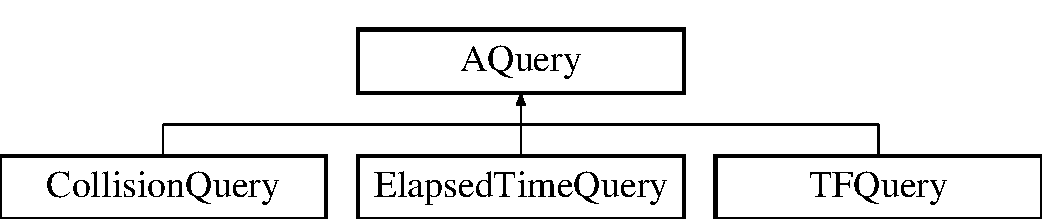
\includegraphics[height=2.000000cm]{structAQuery}
\end{center}
\end{figure}
\subsection*{Public Member Functions}
\begin{DoxyCompactItemize}
\item 
\hypertarget{structAQuery_a69ab1ecccf6747c152b6a82ad455eee7}{{\bfseries A\-Query} (\hyperlink{classGiskardActionServer}{Giskard\-Action\-Server} $\ast$\-\_\-p\-Server, string \-\_\-name)}\label{structAQuery_a69ab1ecccf6747c152b6a82ad455eee7}

\item 
\hypertarget{structAQuery_a11e6e2e3528ddaeac181b3ed323b07e1}{virtual bool {\bfseries eval} ()=0}\label{structAQuery_a11e6e2e3528ddaeac181b3ed323b07e1}

\end{DoxyCompactItemize}
\subsection*{Protected Attributes}
\begin{DoxyCompactItemize}
\item 
const string \hyperlink{structAQuery_a209eec59fbdf038ec7de39db059ddaa4}{name}
\item 
\hyperlink{classGiskardActionServer}{Giskard\-Action\-Server} $\ast$ \hyperlink{structAQuery_ae8c350ae2bc8715fb1e1eec2ff099269}{p\-Server}
\end{DoxyCompactItemize}


\subsection{Detailed Description}
Abstract base class for all action server queries. 

This abstract base class provides the data and function declarations the action server needs from a query to run it. 

\subsection{Member Data Documentation}
\hypertarget{structAQuery_a209eec59fbdf038ec7de39db059ddaa4}{\index{A\-Query@{A\-Query}!name@{name}}
\index{name@{name}!AQuery@{A\-Query}}
\subsubsection[{name}]{\setlength{\rightskip}{0pt plus 5cm}const string A\-Query\-::name\hspace{0.3cm}{\ttfamily [protected]}}}\label{structAQuery_a209eec59fbdf038ec7de39db059ddaa4}
Name of the controller input \hypertarget{structAQuery_ae8c350ae2bc8715fb1e1eec2ff099269}{\index{A\-Query@{A\-Query}!p\-Server@{p\-Server}}
\index{p\-Server@{p\-Server}!AQuery@{A\-Query}}
\subsubsection[{p\-Server}]{\setlength{\rightskip}{0pt plus 5cm}{\bf Giskard\-Action\-Server}$\ast$ A\-Query\-::p\-Server\hspace{0.3cm}{\ttfamily [protected]}}}\label{structAQuery_ae8c350ae2bc8715fb1e1eec2ff099269}
Pointer to the action server 

The documentation for this struct was generated from the following file\-:\begin{DoxyCompactItemize}
\item 
suturo\-\_\-action\-\_\-server/include/suturo\-\_\-action\-\_\-server/Giskard\-Action\-Server.\-h\end{DoxyCompactItemize}

\hypertarget{structCollisionScene_1_1bBox}{\section{Collision\-Scene\-:\-:b\-Box Struct Reference}
\label{structCollisionScene_1_1bBox}\index{Collision\-Scene\-::b\-Box@{Collision\-Scene\-::b\-Box}}
}
\subsection*{Public Member Functions}
\begin{DoxyCompactItemize}
\item 
\hypertarget{structCollisionScene_1_1bBox_ad9f6bbe6943643ba48ba8945ca7d9108}{{\bfseries b\-Box} (float x, float y, float z)}\label{structCollisionScene_1_1bBox_ad9f6bbe6943643ba48ba8945ca7d9108}

\end{DoxyCompactItemize}
\subsection*{Public Attributes}
\begin{DoxyCompactItemize}
\item 
\hypertarget{structCollisionScene_1_1bBox_a29ee0f7ab0c38c25cf8a322b4ef7b641}{float {\bfseries x}}\label{structCollisionScene_1_1bBox_a29ee0f7ab0c38c25cf8a322b4ef7b641}

\item 
\hypertarget{structCollisionScene_1_1bBox_af538879099c49b49d5ed64f28e3a543b}{float {\bfseries y}}\label{structCollisionScene_1_1bBox_af538879099c49b49d5ed64f28e3a543b}

\item 
\hypertarget{structCollisionScene_1_1bBox_a4105da0d12ad900729b712620fb4eba6}{float {\bfseries z}}\label{structCollisionScene_1_1bBox_a4105da0d12ad900729b712620fb4eba6}

\end{DoxyCompactItemize}


The documentation for this struct was generated from the following file\-:\begin{DoxyCompactItemize}
\item 
suturo\-\_\-action\-\_\-server/include/suturo\-\_\-action\-\_\-server/Collision\-Scene.\-h\end{DoxyCompactItemize}

\hypertarget{structCollisionQuery}{\section{Collision\-Query Struct Reference}
\label{structCollisionQuery}\index{Collision\-Query@{Collision\-Query}}
}


Query updating the closest points between a robot link and the surroundings.  




{\ttfamily \#include $<$Giskard\-Action\-Server.\-h$>$}

Inheritance diagram for Collision\-Query\-:\begin{figure}[H]
\begin{center}
\leavevmode
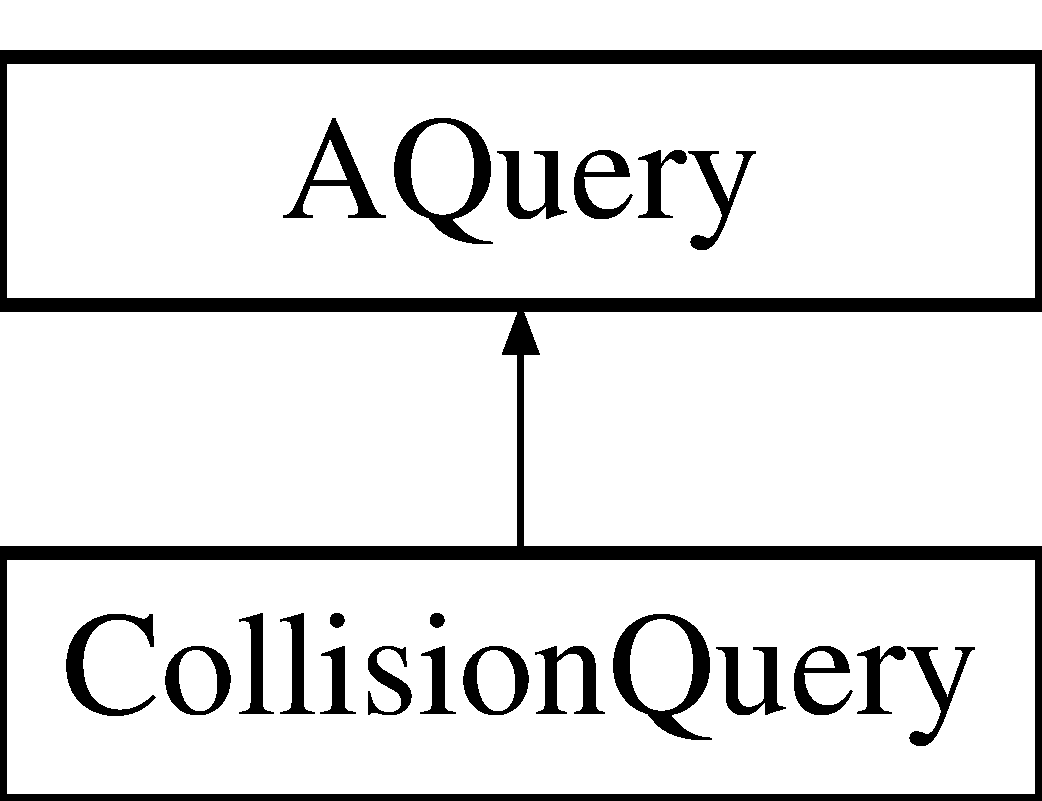
\includegraphics[height=2.000000cm]{structCollisionQuery}
\end{center}
\end{figure}
\subsection*{Public Member Functions}
\begin{DoxyCompactItemize}
\item 
\hypertarget{structCollisionQuery_a684dad7ad6f5c3faedab8e1ffe064515}{{\bfseries Collision\-Query} (\hyperlink{classGiskardActionServer}{Giskard\-Action\-Server} $\ast$\-\_\-p\-Server, string \-\_\-link, \hyperlink{classMutexMap}{Collision\-Scene\-::\-Query\-Map} \&\-\_\-map)}\label{structCollisionQuery_a684dad7ad6f5c3faedab8e1ffe064515}

\item 
\hypertarget{structCollisionQuery_a306f589988aa5e5b455a8bac2467b323}{bool {\bfseries eval} ()}\label{structCollisionQuery_a306f589988aa5e5b455a8bac2467b323}

\end{DoxyCompactItemize}
\subsection*{Private Attributes}
\begin{DoxyCompactItemize}
\item 
const string \hyperlink{structCollisionQuery_ad29d6393aec770b2975e5fe43f121ae1}{link}
\item 
const string \hyperlink{structCollisionQuery_a1f32be858524ab1886b7def2b5cfea69}{on\-\_\-link}
\item 
\hypertarget{structCollisionQuery_ad64ac9509d640282a47d726df7e1849e}{const string {\bfseries in\-\_\-world}}\label{structCollisionQuery_ad64ac9509d640282a47d726df7e1849e}

\item 
\hyperlink{classMutexMap}{Collision\-Scene\-::\-Query\-Map} \& \hyperlink{structCollisionQuery_a014c3155faa91f550e82d6cf70cc1670}{map}
\end{DoxyCompactItemize}
\subsection*{Additional Inherited Members}


\subsection{Detailed Description}
Query updating the closest points between a robot link and the surroundings. 

\subsection{Member Data Documentation}
\hypertarget{structCollisionQuery_ad29d6393aec770b2975e5fe43f121ae1}{\index{Collision\-Query@{Collision\-Query}!link@{link}}
\index{link@{link}!CollisionQuery@{Collision\-Query}}
\subsubsection[{link}]{\setlength{\rightskip}{0pt plus 5cm}const string Collision\-Query\-::link\hspace{0.3cm}{\ttfamily [private]}}}\label{structCollisionQuery_ad29d6393aec770b2975e5fe43f121ae1}
Name of the link \hypertarget{structCollisionQuery_a014c3155faa91f550e82d6cf70cc1670}{\index{Collision\-Query@{Collision\-Query}!map@{map}}
\index{map@{map}!CollisionQuery@{Collision\-Query}}
\subsubsection[{map}]{\setlength{\rightskip}{0pt plus 5cm}{\bf Collision\-Scene\-::\-Query\-Map}\& Collision\-Query\-::map\hspace{0.3cm}{\ttfamily [private]}}}\label{structCollisionQuery_a014c3155faa91f550e82d6cf70cc1670}
Result map of collision scene \hypertarget{structCollisionQuery_a1f32be858524ab1886b7def2b5cfea69}{\index{Collision\-Query@{Collision\-Query}!on\-\_\-link@{on\-\_\-link}}
\index{on\-\_\-link@{on\-\_\-link}!CollisionQuery@{Collision\-Query}}
\subsubsection[{on\-\_\-link}]{\setlength{\rightskip}{0pt plus 5cm}const string Collision\-Query\-::on\-\_\-link\hspace{0.3cm}{\ttfamily [private]}}}\label{structCollisionQuery_a1f32be858524ab1886b7def2b5cfea69}
Names of the inputs 

The documentation for this struct was generated from the following file\-:\begin{DoxyCompactItemize}
\item 
suturo\-\_\-action\-\_\-server/include/suturo\-\_\-action\-\_\-server/Giskard\-Action\-Server.\-h\end{DoxyCompactItemize}

\hypertarget{classCollisionScene}{\section{Collision\-Scene Class Reference}
\label{classCollisionScene}\index{Collision\-Scene@{Collision\-Scene}}
}
\subsection*{Classes}
\begin{DoxyCompactItemize}
\item 
struct \hyperlink{structCollisionScene_1_1bBox}{b\-Box}
\item 
struct \hyperlink{structCollisionScene_1_1SQueryPoints}{S\-Query\-Points}
\item 
struct \hyperlink{structCollisionScene_1_1SRobotLink}{S\-Robot\-Link}
\end{DoxyCompactItemize}
\subsection*{Public Types}
\begin{DoxyCompactItemize}
\item 
\hypertarget{classCollisionScene_aa0b9e7bae731b946f0e049b4591bbaf4}{typedef \hyperlink{classMutexMap}{Mutex\-Map}$<$ string, \\*
\hyperlink{structCollisionScene_1_1SQueryPoints}{Collision\-Scene\-::\-S\-Query\-Points} $>$ {\bfseries Query\-Map}}\label{classCollisionScene_aa0b9e7bae731b946f0e049b4591bbaf4}

\end{DoxyCompactItemize}
\subsection*{Public Member Functions}
\begin{DoxyCompactItemize}
\item 
\hyperlink{classCollisionScene_ad814c6de8d0c1b6c3c9cf8e75ea19358}{Collision\-Scene} (\hyperlink{classMutexMap}{Query\-Map} \&\-\_\-map)
\begin{DoxyCompactList}\small\item\em Constructs the \hyperlink{classCollisionScene}{Collision\-Scene}. \end{DoxyCompactList}\item 
\hypertarget{classCollisionScene_a78292b107e0ba4d074749e8a45e52ae3}{\hyperlink{classCollisionScene_a78292b107e0ba4d074749e8a45e52ae3}{$\sim$\-Collision\-Scene} ()}\label{classCollisionScene_a78292b107e0ba4d074749e8a45e52ae3}

\begin{DoxyCompactList}\small\item\em Stops the update thread and deletes the octree. \end{DoxyCompactList}\item 
void \hyperlink{classCollisionScene_a76efb9371fd01bb1a372ddc9535f9537}{set\-Robot\-Description} (const string \&urdf\-Str)
\begin{DoxyCompactList}\small\item\em Sets the robot description. \end{DoxyCompactList}\item 
void \hyperlink{classCollisionScene_ad7e104a8659e5eb0c9f55c56b6f9011d}{add\-Query\-Link} (const string \&link)
\begin{DoxyCompactList}\small\item\em Adds a query link to the \hyperlink{classCollisionScene}{Collision\-Scene}. \end{DoxyCompactList}\item 
\hypertarget{classCollisionScene_aa1d80c51501b53bf176f1484fba7d3bd}{void {\bfseries clear\-Query\-Links} ()}\label{classCollisionScene_aa1d80c51501b53bf176f1484fba7d3bd}

\item 
\hypertarget{classCollisionScene_a0d1d5b732e65711bd783b27a9b866219}{void \hyperlink{classCollisionScene_a0d1d5b732e65711bd783b27a9b866219}{update\-Query} ()}\label{classCollisionScene_a0d1d5b732e65711bd783b27a9b866219}

\begin{DoxyCompactList}\small\item\em updates the \hyperlink{structCollisionScene_1_1SQueryPoints}{S\-Query\-Points} for every link in the \hyperlink{classCollisionScene}{Collision\-Scene}. \end{DoxyCompactList}\item 
\hypertarget{classCollisionScene_a35fffc2c243b08deac3914d2b0c80169}{void \hyperlink{classCollisionScene_a35fffc2c243b08deac3914d2b0c80169}{update\-Bboxes} ()}\label{classCollisionScene_a35fffc2c243b08deac3914d2b0c80169}

\begin{DoxyCompactList}\small\item\em updates the bounding boxes of every query link in the \hyperlink{classCollisionScene}{Collision\-Scene}. \end{DoxyCompactList}\end{DoxyCompactItemize}
\subsection*{Private Member Functions}
\begin{DoxyCompactItemize}
\item 
void \hyperlink{classCollisionScene_a338284876502577c783b745ba7bac385}{traverse\-Tree} (\hyperlink{structCollisionScene_1_1SQueryPoints}{S\-Query\-Points} \&q\-Point, const Eigen\-::\-Affine3d t\-Link, const \hyperlink{structCollisionScene_1_1bBox}{b\-Box} \&link\-Box)
\begin{DoxyCompactList}\small\item\em iterates over every leaf of the octree to find the closest voxel to the link. \end{DoxyCompactList}\item 
Eigen\-::\-Vector3d \hyperlink{classCollisionScene_a287195084a9b8dd1eb7fbbf093766eb1}{calc\-Intersection} (const Eigen\-::\-Vector3d \&v, const struct \hyperlink{structCollisionScene_1_1bBox}{b\-Box} \&box)
\begin{DoxyCompactList}\small\item\em Calculates the intersection of a Vector from the center of the bounding box and the bounding box. \end{DoxyCompactList}\item 
void \hyperlink{classCollisionScene_a16b5e86c6b438cee575dbafb47506970}{update\-Point\-Cloud} (const pcl\-::\-Point\-Cloud$<$ pcl\-::\-Point\-X\-Y\-Z\-R\-G\-B $>$\-::Const\-Ptr \&input)
\begin{DoxyCompactList}\small\item\em Makes a copy of the point cloud to the point cloud pointer. \end{DoxyCompactList}\item 
void \hyperlink{classCollisionScene_a0458b7a7748c991626e7154b6cacbd0a}{set\-Ref\-Frame} (const string \&p\-Ref\-Frame)
\begin{DoxyCompactList}\small\item\em Sets the reference frame of the \hyperlink{classCollisionScene}{Collision\-Scene}. \end{DoxyCompactList}\item 
\hypertarget{classCollisionScene_a493a467161c0bab5d6717f58d96d3e00}{void \hyperlink{classCollisionScene_a493a467161c0bab5d6717f58d96d3e00}{update\-Octree\-Visualization} ()}\label{classCollisionScene_a493a467161c0bab5d6717f58d96d3e00}

\begin{DoxyCompactList}\small\item\em Publishes the leaf nodes of the octree as marker. \end{DoxyCompactList}\item 
\hypertarget{classCollisionScene_aa33eb3f701cfd4d750cfedec58bc9729}{void \hyperlink{classCollisionScene_aa33eb3f701cfd4d750cfedec58bc9729}{update\-Octree\-Thread} ()}\label{classCollisionScene_aa33eb3f701cfd4d750cfedec58bc9729}

\begin{DoxyCompactList}\small\item\em Updates the octree when a new point cloud arrives. \end{DoxyCompactList}\item 
\hypertarget{classCollisionScene_ae6d94b627968a2508cd2ac43a83cf1bf}{void \hyperlink{classCollisionScene_ae6d94b627968a2508cd2ac43a83cf1bf}{swap\-Point\-Clouds} ()}\label{classCollisionScene_ae6d94b627968a2508cd2ac43a83cf1bf}

\begin{DoxyCompactList}\small\item\em Swaps the pointers of the active and inactive point cloud. \end{DoxyCompactList}\end{DoxyCompactItemize}
\subsection*{Private Attributes}
\begin{DoxyCompactItemize}
\item 
\hypertarget{classCollisionScene_a30b43dd54810ba4ba85ce0736b061c45}{ros\-::\-Node\-Handle {\bfseries nh}}\label{classCollisionScene_a30b43dd54810ba4ba85ce0736b061c45}

\item 
\hypertarget{classCollisionScene_afaf7a12837bb9694b0df4d2a3888405d}{ros\-::\-Callback\-Queue {\bfseries cb\-Queue}}\label{classCollisionScene_afaf7a12837bb9694b0df4d2a3888405d}

\item 
\hypertarget{classCollisionScene_ac715ff5694a1b35aea05835c9c50716d}{ros\-::\-Timer {\bfseries update\-Timer}}\label{classCollisionScene_ac715ff5694a1b35aea05835c9c50716d}

\item 
int \hyperlink{classCollisionScene_a7b106dc5a0338af700abaf62d6d77ad9}{octree\-Depth} = 6
\item 
int \hyperlink{classCollisionScene_aa50f77359129b8a44335d76ee3420cc7}{octree\-Size} = 2
\item 
\hypertarget{classCollisionScene_acad20b472c7f6a8acd6fafcaa9fe35e5}{bool {\bfseries swap} = false}\label{classCollisionScene_acad20b472c7f6a8acd6fafcaa9fe35e5}

\item 
\hypertarget{classCollisionScene_a0bf30bd2de0b64092e215f0d1e45a28a}{bool {\bfseries stop\-Update\-Thread}}\label{classCollisionScene_a0bf30bd2de0b64092e215f0d1e45a28a}

\item 
\hypertarget{classCollisionScene_a1d885afac5e533d6972b31148c22fc35}{pcl\-::\-Point\-Cloud\\*
$<$ pcl\-::\-Point\-X\-Y\-Z\-R\-G\-B $>$\-::Const\-Ptr {\bfseries active\-Point\-Cloud\-Pointer}}\label{classCollisionScene_a1d885afac5e533d6972b31148c22fc35}

\item 
\hypertarget{classCollisionScene_aee8373f709dd3efa1300f676f783d2bc}{pcl\-::\-Point\-Cloud\\*
$<$ pcl\-::\-Point\-X\-Y\-Z\-R\-G\-B $>$\-::Const\-Ptr {\bfseries point\-Cloud\-Pointer}}\label{classCollisionScene_aee8373f709dd3efa1300f676f783d2bc}

\item 
std\-::thread \hyperlink{classCollisionScene_af8a098eaddd613c3312f63c4b6a99a1a}{t}
\item 
\hypertarget{classCollisionScene_acec1a566d8788d3d6de7da58dcb80ec4}{ros\-::\-Publisher {\bfseries octree\-Vis\-Publisher}}\label{classCollisionScene_acec1a566d8788d3d6de7da58dcb80ec4}

\item 
\hypertarget{classCollisionScene_ae185f726a5ec8c68f92980eace1b613b}{ros\-::\-Subscriber {\bfseries point\-Cloud\-Subscriber}}\label{classCollisionScene_ae185f726a5ec8c68f92980eace1b613b}

\item 
\hypertarget{classCollisionScene_a09c519cf1c97e9e1c4d5d90197b8b404}{urdf\-::\-Model {\bfseries robot}}\label{classCollisionScene_a09c519cf1c97e9e1c4d5d90197b8b404}

\item 
unordered\-\_\-map$<$ string, \hyperlink{structCollisionScene_1_1bBox}{b\-Box} $>$ \hyperlink{classCollisionScene_a86929e1d07a315dec9e6c1b305cacabc}{bbox\-Map}
\item 
\hyperlink{classMutexMap}{Query\-Map} \& \hyperlink{classCollisionScene_a50300cec4b2a8bb3c3d51eef54acc0f8}{map}
\item 
set$<$ string $>$ \hyperlink{classCollisionScene_ab6fe95cec3f4207074aabedce8b4be61}{links}
\item 
\hypertarget{classCollisionScene_acf1bebb09bc150915efbb88ced9e3db1}{tf\-::\-Transform\-Listener {\bfseries tf\-Listener}}\label{classCollisionScene_acf1bebb09bc150915efbb88ced9e3db1}

\item 
\hypertarget{classCollisionScene_a59692641d55fc7b2c680429030749365}{string {\bfseries controller\-Ref\-Frame}}\label{classCollisionScene_a59692641d55fc7b2c680429030749365}

\item 
\hypertarget{classCollisionScene_a53afa27e7913804dfe9b77c72ff55c7a}{string {\bfseries octomap\-Frame} = \char`\"{}head\-\_\-mount\-\_\-kinect\-\_\-rgb\-\_\-optical\-\_\-frame\char`\"{}}\label{classCollisionScene_a53afa27e7913804dfe9b77c72ff55c7a}

\item 
\hypertarget{classCollisionScene_a7fae33d8e04f4b7db02b14e78220b9a4}{\hyperlink{classsuturo__octree_1_1Octree}{suturo\-\_\-octree\-::\-Octree} $\ast$ {\bfseries octree} = N\-U\-L\-L}\label{classCollisionScene_a7fae33d8e04f4b7db02b14e78220b9a4}

\item 
\hypertarget{classCollisionScene_a9957ef59711be6baa110dc8483c58afe}{mutex {\bfseries point\-Cloud\-Mutex}}\label{classCollisionScene_a9957ef59711be6baa110dc8483c58afe}

\end{DoxyCompactItemize}


\subsection{Constructor \& Destructor Documentation}
\hypertarget{classCollisionScene_ad814c6de8d0c1b6c3c9cf8e75ea19358}{\index{Collision\-Scene@{Collision\-Scene}!Collision\-Scene@{Collision\-Scene}}
\index{Collision\-Scene@{Collision\-Scene}!CollisionScene@{Collision\-Scene}}
\subsubsection[{Collision\-Scene}]{\setlength{\rightskip}{0pt plus 5cm}Collision\-Scene\-::\-Collision\-Scene (
\begin{DoxyParamCaption}
\item[{{\bf Query\-Map} \&}]{\-\_\-map}
\end{DoxyParamCaption}
)}}\label{classCollisionScene_ad814c6de8d0c1b6c3c9cf8e75ea19358}


Constructs the \hyperlink{classCollisionScene}{Collision\-Scene}. 


\begin{DoxyParams}{Parameters}
{\em \-\_\-map} & The mutex map which maps \hyperlink{structCollisionScene_1_1SQueryPoints}{S\-Query\-Points} to the query links \\
\hline
\end{DoxyParams}


\subsection{Member Function Documentation}
\hypertarget{classCollisionScene_ad7e104a8659e5eb0c9f55c56b6f9011d}{\index{Collision\-Scene@{Collision\-Scene}!add\-Query\-Link@{add\-Query\-Link}}
\index{add\-Query\-Link@{add\-Query\-Link}!CollisionScene@{Collision\-Scene}}
\subsubsection[{add\-Query\-Link}]{\setlength{\rightskip}{0pt plus 5cm}void Collision\-Scene\-::add\-Query\-Link (
\begin{DoxyParamCaption}
\item[{const string \&}]{link}
\end{DoxyParamCaption}
)}}\label{classCollisionScene_ad7e104a8659e5eb0c9f55c56b6f9011d}


Adds a query link to the \hyperlink{classCollisionScene}{Collision\-Scene}. 


\begin{DoxyParams}[1]{Parameters}
\mbox{\tt in}  & {\em link} & The query link \\
\hline
\end{DoxyParams}
\hypertarget{classCollisionScene_a287195084a9b8dd1eb7fbbf093766eb1}{\index{Collision\-Scene@{Collision\-Scene}!calc\-Intersection@{calc\-Intersection}}
\index{calc\-Intersection@{calc\-Intersection}!CollisionScene@{Collision\-Scene}}
\subsubsection[{calc\-Intersection}]{\setlength{\rightskip}{0pt plus 5cm}Vector3d Collision\-Scene\-::calc\-Intersection (
\begin{DoxyParamCaption}
\item[{const Eigen\-::\-Vector3d \&}]{v, }
\item[{const struct {\bf b\-Box} \&}]{box}
\end{DoxyParamCaption}
)\hspace{0.3cm}{\ttfamily [private]}}}\label{classCollisionScene_a287195084a9b8dd1eb7fbbf093766eb1}


Calculates the intersection of a Vector from the center of the bounding box and the bounding box. 


\begin{DoxyParams}[1]{Parameters}
\mbox{\tt in}  & {\em v} & The Vector from the center of the bounding box \\
\hline
\mbox{\tt in}  & {\em box} & The box\\
\hline
\end{DoxyParams}
\begin{DoxyReturn}{Returns}
The intersection. 
\end{DoxyReturn}
\hypertarget{classCollisionScene_a0458b7a7748c991626e7154b6cacbd0a}{\index{Collision\-Scene@{Collision\-Scene}!set\-Ref\-Frame@{set\-Ref\-Frame}}
\index{set\-Ref\-Frame@{set\-Ref\-Frame}!CollisionScene@{Collision\-Scene}}
\subsubsection[{set\-Ref\-Frame}]{\setlength{\rightskip}{0pt plus 5cm}void Collision\-Scene\-::set\-Ref\-Frame (
\begin{DoxyParamCaption}
\item[{const string \&}]{pcontroller\-Ref\-Frame}
\end{DoxyParamCaption}
)\hspace{0.3cm}{\ttfamily [private]}}}\label{classCollisionScene_a0458b7a7748c991626e7154b6cacbd0a}


Sets the reference frame of the \hyperlink{classCollisionScene}{Collision\-Scene}. 


\begin{DoxyParams}[1]{Parameters}
\mbox{\tt in}  & {\em p\-Ref\-Frame} & The reference frame \\
\hline
\end{DoxyParams}
\hypertarget{classCollisionScene_a76efb9371fd01bb1a372ddc9535f9537}{\index{Collision\-Scene@{Collision\-Scene}!set\-Robot\-Description@{set\-Robot\-Description}}
\index{set\-Robot\-Description@{set\-Robot\-Description}!CollisionScene@{Collision\-Scene}}
\subsubsection[{set\-Robot\-Description}]{\setlength{\rightskip}{0pt plus 5cm}void Collision\-Scene\-::set\-Robot\-Description (
\begin{DoxyParamCaption}
\item[{const string \&}]{urdf\-Str}
\end{DoxyParamCaption}
)}}\label{classCollisionScene_a76efb9371fd01bb1a372ddc9535f9537}


Sets the robot description. 


\begin{DoxyParams}[1]{Parameters}
\mbox{\tt in}  & {\em urdf\-Str} & The urdf string \\
\hline
\end{DoxyParams}
\hypertarget{classCollisionScene_a338284876502577c783b745ba7bac385}{\index{Collision\-Scene@{Collision\-Scene}!traverse\-Tree@{traverse\-Tree}}
\index{traverse\-Tree@{traverse\-Tree}!CollisionScene@{Collision\-Scene}}
\subsubsection[{traverse\-Tree}]{\setlength{\rightskip}{0pt plus 5cm}void Collision\-Scene\-::traverse\-Tree (
\begin{DoxyParamCaption}
\item[{{\bf S\-Query\-Points} \&}]{q\-Point, }
\item[{const Eigen\-::\-Affine3d}]{t\-Link, }
\item[{const {\bf b\-Box} \&}]{link\-Box}
\end{DoxyParamCaption}
)\hspace{0.3cm}{\ttfamily [private]}}}\label{classCollisionScene_a338284876502577c783b745ba7bac385}


iterates over every leaf of the octree to find the closest voxel to the link. 


\begin{DoxyParams}[1]{Parameters}
 & {\em q\-Point} & The \hyperlink{structCollisionScene_1_1SQueryPoints}{S\-Query\-Points} for the link \\
\hline
\mbox{\tt in}  & {\em t\-Link} & The transform for the link \\
\hline
\mbox{\tt in}  & {\em link\-Box} & The bounding box for the link \\
\hline
\end{DoxyParams}
\hypertarget{classCollisionScene_a16b5e86c6b438cee575dbafb47506970}{\index{Collision\-Scene@{Collision\-Scene}!update\-Point\-Cloud@{update\-Point\-Cloud}}
\index{update\-Point\-Cloud@{update\-Point\-Cloud}!CollisionScene@{Collision\-Scene}}
\subsubsection[{update\-Point\-Cloud}]{\setlength{\rightskip}{0pt plus 5cm}void Collision\-Scene\-::update\-Point\-Cloud (
\begin{DoxyParamCaption}
\item[{const pcl\-::\-Point\-Cloud$<$ pcl\-::\-Point\-X\-Y\-Z\-R\-G\-B $>$\-::Const\-Ptr \&}]{input}
\end{DoxyParamCaption}
)\hspace{0.3cm}{\ttfamily [private]}}}\label{classCollisionScene_a16b5e86c6b438cee575dbafb47506970}


Makes a copy of the point cloud to the point cloud pointer. 


\begin{DoxyParams}[1]{Parameters}
\mbox{\tt in}  & {\em input} & The point cloud message \\
\hline
\end{DoxyParams}


\subsection{Member Data Documentation}
\hypertarget{classCollisionScene_a86929e1d07a315dec9e6c1b305cacabc}{\index{Collision\-Scene@{Collision\-Scene}!bbox\-Map@{bbox\-Map}}
\index{bbox\-Map@{bbox\-Map}!CollisionScene@{Collision\-Scene}}
\subsubsection[{bbox\-Map}]{\setlength{\rightskip}{0pt plus 5cm}unordered\-\_\-map$<$string, {\bf b\-Box}$>$ Collision\-Scene\-::bbox\-Map\hspace{0.3cm}{\ttfamily [private]}}}\label{classCollisionScene_a86929e1d07a315dec9e6c1b305cacabc}
This map contains the bounding boxes for each link. \hypertarget{classCollisionScene_ab6fe95cec3f4207074aabedce8b4be61}{\index{Collision\-Scene@{Collision\-Scene}!links@{links}}
\index{links@{links}!CollisionScene@{Collision\-Scene}}
\subsubsection[{links}]{\setlength{\rightskip}{0pt plus 5cm}set$<$string$>$ Collision\-Scene\-::links\hspace{0.3cm}{\ttfamily [private]}}}\label{classCollisionScene_ab6fe95cec3f4207074aabedce8b4be61}
The set of all the links with collision queries. \hypertarget{classCollisionScene_a50300cec4b2a8bb3c3d51eef54acc0f8}{\index{Collision\-Scene@{Collision\-Scene}!map@{map}}
\index{map@{map}!CollisionScene@{Collision\-Scene}}
\subsubsection[{map}]{\setlength{\rightskip}{0pt plus 5cm}{\bf Query\-Map}\& Collision\-Scene\-::map\hspace{0.3cm}{\ttfamily [private]}}}\label{classCollisionScene_a50300cec4b2a8bb3c3d51eef54acc0f8}
The mutex map which maps \hyperlink{structCollisionScene_1_1SQueryPoints}{S\-Query\-Points} to the query links. \hypertarget{classCollisionScene_a7b106dc5a0338af700abaf62d6d77ad9}{\index{Collision\-Scene@{Collision\-Scene}!octree\-Depth@{octree\-Depth}}
\index{octree\-Depth@{octree\-Depth}!CollisionScene@{Collision\-Scene}}
\subsubsection[{octree\-Depth}]{\setlength{\rightskip}{0pt plus 5cm}int Collision\-Scene\-::octree\-Depth = 6\hspace{0.3cm}{\ttfamily [private]}}}\label{classCollisionScene_a7b106dc5a0338af700abaf62d6d77ad9}
The depth of the octree. A depth greater than 7 is not recommended due to memory consumption. \hypertarget{classCollisionScene_aa50f77359129b8a44335d76ee3420cc7}{\index{Collision\-Scene@{Collision\-Scene}!octree\-Size@{octree\-Size}}
\index{octree\-Size@{octree\-Size}!CollisionScene@{Collision\-Scene}}
\subsubsection[{octree\-Size}]{\setlength{\rightskip}{0pt plus 5cm}int Collision\-Scene\-::octree\-Size = 2\hspace{0.3cm}{\ttfamily [private]}}}\label{classCollisionScene_aa50f77359129b8a44335d76ee3420cc7}
The size of the octree in m. \hypertarget{classCollisionScene_af8a098eaddd613c3312f63c4b6a99a1a}{\index{Collision\-Scene@{Collision\-Scene}!t@{t}}
\index{t@{t}!CollisionScene@{Collision\-Scene}}
\subsubsection[{t}]{\setlength{\rightskip}{0pt plus 5cm}std\-::thread Collision\-Scene\-::t\hspace{0.3cm}{\ttfamily [private]}}}\label{classCollisionScene_af8a098eaddd613c3312f63c4b6a99a1a}
The octree update thread. 

The documentation for this class was generated from the following files\-:\begin{DoxyCompactItemize}
\item 
suturo\-\_\-action\-\_\-server/include/suturo\-\_\-action\-\_\-server/Collision\-Scene.\-h\item 
suturo\-\_\-action\-\_\-server/src/Collision\-Scene.\-cpp\end{DoxyCompactItemize}

\hypertarget{classgiskard__suturo_1_1ConcatListSpec}{\section{giskard\-\_\-suturo\-:\-:Concat\-List\-Spec Class Reference}
\label{classgiskard__suturo_1_1ConcatListSpec}\index{giskard\-\_\-suturo\-::\-Concat\-List\-Spec@{giskard\-\_\-suturo\-::\-Concat\-List\-Spec}}
}


Specification for list concatenation.  




{\ttfamily \#include $<$specifications.\-h$>$}

Inheritance diagram for giskard\-\_\-suturo\-:\-:Concat\-List\-Spec\-:\begin{figure}[H]
\begin{center}
\leavevmode
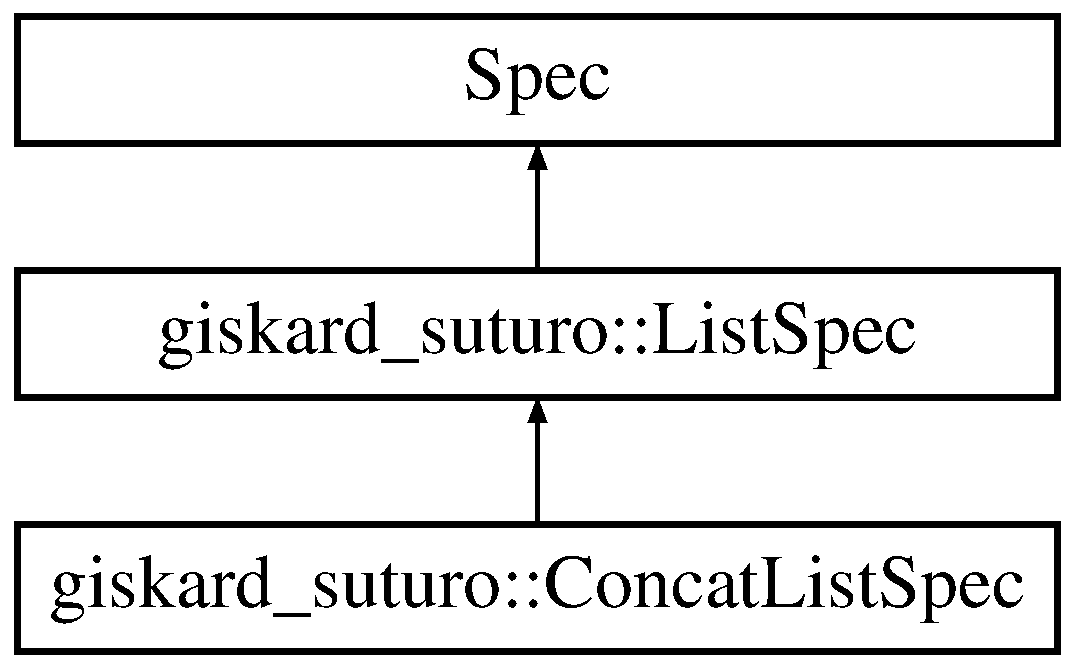
\includegraphics[height=3.000000cm]{classgiskard__suturo_1_1ConcatListSpec}
\end{center}
\end{figure}
\subsection*{Public Member Functions}
\begin{DoxyCompactItemize}
\item 
\hypertarget{classgiskard__suturo_1_1ConcatListSpec_a7c8f8282724b87929570412fb549c2e5}{{\bfseries Concat\-List\-Spec} (const List\-Spec\-Ptr \&\-\_\-lhs, const List\-Spec\-Ptr \&\-\_\-rhs)}\label{classgiskard__suturo_1_1ConcatListSpec_a7c8f8282724b87929570412fb549c2e5}

\item 
const Spec\-Ptr \hyperlink{classgiskard__suturo_1_1ConcatListSpec_ab4c15638659af22f9bfc4676e4e7b399}{inner\-Type} () const 
\begin{DoxyCompactList}\small\item\em Returns pointer determining the type of the list's contents. \end{DoxyCompactList}\item 
\hypertarget{classgiskard__suturo_1_1ConcatListSpec_acaaf348a330e3f86b51f098bbd7a973a}{bool {\bfseries equals} (const Spec \&other) const }\label{classgiskard__suturo_1_1ConcatListSpec_acaaf348a330e3f86b51f098bbd7a973a}

\item 
\hypertarget{classgiskard__suturo_1_1ConcatListSpec_aef3425780757d93d5b6ad666643c45f0}{void {\bfseries set\-\_\-lhs} (const List\-Spec\-Ptr \&\-\_\-lhs)}\label{classgiskard__suturo_1_1ConcatListSpec_aef3425780757d93d5b6ad666643c45f0}

\item 
\hypertarget{classgiskard__suturo_1_1ConcatListSpec_ac1245b7bf9645ead2c6021b0faa753a0}{void {\bfseries set\-\_\-rhs} (const List\-Spec\-Ptr \&\-\_\-rhs)}\label{classgiskard__suturo_1_1ConcatListSpec_ac1245b7bf9645ead2c6021b0faa753a0}

\item 
\hypertarget{classgiskard__suturo_1_1ConcatListSpec_a0a6773bd81f475f01412f73f478b2d77}{const List\-Spec\-Ptr \& {\bfseries get\-\_\-lhs} () const }\label{classgiskard__suturo_1_1ConcatListSpec_a0a6773bd81f475f01412f73f478b2d77}

\item 
\hypertarget{classgiskard__suturo_1_1ConcatListSpec_a3f2e02bf25953434a90f00139b3294c9}{const List\-Spec\-Ptr \& {\bfseries get\-\_\-rhs} () const }\label{classgiskard__suturo_1_1ConcatListSpec_a3f2e02bf25953434a90f00139b3294c9}

\item 
\hypertarget{classgiskard__suturo_1_1ConcatListSpec_a4fa8c3dd54a310d0b99e823330847b6b}{std\-::vector$<$ Spec\-Ptr $>$ {\bfseries get\-\_\-value} () const }\label{classgiskard__suturo_1_1ConcatListSpec_a4fa8c3dd54a310d0b99e823330847b6b}

\item 
\hypertarget{classgiskard__suturo_1_1ConcatListSpec_a386b7b02523ef77bb6c1c2ad688ea09d}{void {\bfseries get\-\_\-input\-\_\-specs} (std\-::vector$<$ const Input\-Spec $\ast$ $>$ \&inputs) const }\label{classgiskard__suturo_1_1ConcatListSpec_a386b7b02523ef77bb6c1c2ad688ea09d}

\end{DoxyCompactItemize}
\subsection*{Private Attributes}
\begin{DoxyCompactItemize}
\item 
\hypertarget{classgiskard__suturo_1_1ConcatListSpec_a7fef95cd6895828dc71ed75615137eaf}{List\-Spec\-Ptr {\bfseries lhs}}\label{classgiskard__suturo_1_1ConcatListSpec_a7fef95cd6895828dc71ed75615137eaf}

\item 
\hypertarget{classgiskard__suturo_1_1ConcatListSpec_a582bd70723973e89c7c3cfecba622e34}{List\-Spec\-Ptr {\bfseries rhs}}\label{classgiskard__suturo_1_1ConcatListSpec_a582bd70723973e89c7c3cfecba622e34}

\end{DoxyCompactItemize}


\subsection{Detailed Description}
Specification for list concatenation. 

\subsection{Member Function Documentation}
\hypertarget{classgiskard__suturo_1_1ConcatListSpec_ab4c15638659af22f9bfc4676e4e7b399}{\index{giskard\-\_\-suturo\-::\-Concat\-List\-Spec@{giskard\-\_\-suturo\-::\-Concat\-List\-Spec}!inner\-Type@{inner\-Type}}
\index{inner\-Type@{inner\-Type}!giskard_suturo::ConcatListSpec@{giskard\-\_\-suturo\-::\-Concat\-List\-Spec}}
\subsubsection[{inner\-Type}]{\setlength{\rightskip}{0pt plus 5cm}const Spec\-Ptr giskard\-\_\-suturo\-::\-Concat\-List\-Spec\-::inner\-Type (
\begin{DoxyParamCaption}
{}
\end{DoxyParamCaption}
) const\hspace{0.3cm}{\ttfamily [inline]}, {\ttfamily [virtual]}}}\label{classgiskard__suturo_1_1ConcatListSpec_ab4c15638659af22f9bfc4676e4e7b399}


Returns pointer determining the type of the list's contents. 

\begin{DoxyReturn}{Returns}
Type pointer 
\end{DoxyReturn}


Implements \hyperlink{classgiskard__suturo_1_1ListSpec_aba0a625da0d48e702aa723fb6fb3bc7e}{giskard\-\_\-suturo\-::\-List\-Spec}.



The documentation for this class was generated from the following files\-:\begin{DoxyCompactItemize}
\item 
giskard\-\_\-suturo\-\_\-parser/include/giskard\-\_\-suturo\-\_\-parser/specifications.\-h\item 
giskard\-\_\-suturo\-\_\-parser/src/specifications.\-cpp\end{DoxyCompactItemize}

\hypertarget{classgiskard__suturo_1_1ConcatStringSpec}{\section{giskard\-\_\-suturo\-:\-:Concat\-String\-Spec Class Reference}
\label{classgiskard__suturo_1_1ConcatStringSpec}\index{giskard\-\_\-suturo\-::\-Concat\-String\-Spec@{giskard\-\_\-suturo\-::\-Concat\-String\-Spec}}
}


Specification for string concatenation.  




{\ttfamily \#include $<$specifications.\-h$>$}

Inheritance diagram for giskard\-\_\-suturo\-:\-:Concat\-String\-Spec\-:\begin{figure}[H]
\begin{center}
\leavevmode
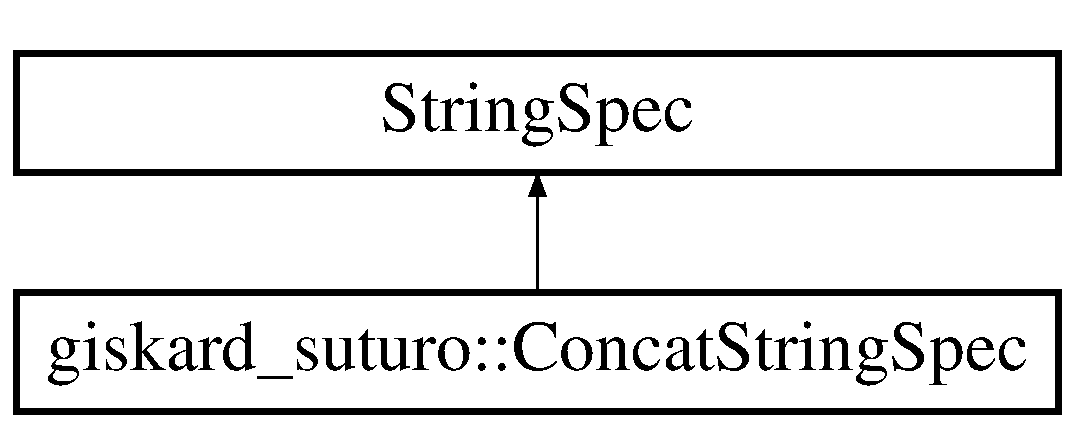
\includegraphics[height=2.000000cm]{classgiskard__suturo_1_1ConcatStringSpec}
\end{center}
\end{figure}
\subsection*{Public Member Functions}
\begin{DoxyCompactItemize}
\item 
\hypertarget{classgiskard__suturo_1_1ConcatStringSpec_a0b8d5a0c2a61926325669d0d709b8d9a}{{\bfseries Concat\-String\-Spec} (const String\-Spec\-Ptr \&\-\_\-lhs, const String\-Spec\-Ptr \&\-\_\-rhs)}\label{classgiskard__suturo_1_1ConcatStringSpec_a0b8d5a0c2a61926325669d0d709b8d9a}

\item 
\hypertarget{classgiskard__suturo_1_1ConcatStringSpec_aefc0b111d6ee941e10d03e4931d8995b}{bool {\bfseries equals} (const Spec \&other) const }\label{classgiskard__suturo_1_1ConcatStringSpec_aefc0b111d6ee941e10d03e4931d8995b}

\item 
\hypertarget{classgiskard__suturo_1_1ConcatStringSpec_ab6c037eb7ce4bf0bd84e53970d651221}{void {\bfseries set\-\_\-lhs} (const String\-Spec\-Ptr \&\-\_\-lhs)}\label{classgiskard__suturo_1_1ConcatStringSpec_ab6c037eb7ce4bf0bd84e53970d651221}

\item 
\hypertarget{classgiskard__suturo_1_1ConcatStringSpec_ad615f74c07e64b711b56a2ad4e5910f8}{void {\bfseries set\-\_\-rhs} (const String\-Spec\-Ptr \&\-\_\-rhs)}\label{classgiskard__suturo_1_1ConcatStringSpec_ad615f74c07e64b711b56a2ad4e5910f8}

\item 
\hypertarget{classgiskard__suturo_1_1ConcatStringSpec_ab6cb19aa13a159072231fb6ff3a0b1b8}{const String\-Spec\-Ptr \& {\bfseries get\-\_\-lhs} () const }\label{classgiskard__suturo_1_1ConcatStringSpec_ab6cb19aa13a159072231fb6ff3a0b1b8}

\item 
\hypertarget{classgiskard__suturo_1_1ConcatStringSpec_ac03a56e5989f4747b047d873d93e1efc}{const String\-Spec\-Ptr \& {\bfseries get\-\_\-rhs} () const }\label{classgiskard__suturo_1_1ConcatStringSpec_ac03a56e5989f4747b047d873d93e1efc}

\item 
\hypertarget{classgiskard__suturo_1_1ConcatStringSpec_a5a0695881b721252a5c97e5cb4a0956d}{std\-::string {\bfseries get\-\_\-value} () const }\label{classgiskard__suturo_1_1ConcatStringSpec_a5a0695881b721252a5c97e5cb4a0956d}

\item 
\hypertarget{classgiskard__suturo_1_1ConcatStringSpec_a778ac0bcc93a4007f008d00aa00febd3}{void {\bfseries get\-\_\-input\-\_\-specs} (std\-::vector$<$ const Input\-Spec $\ast$ $>$ \&inputs) const }\label{classgiskard__suturo_1_1ConcatStringSpec_a778ac0bcc93a4007f008d00aa00febd3}

\end{DoxyCompactItemize}
\subsection*{Private Attributes}
\begin{DoxyCompactItemize}
\item 
\hypertarget{classgiskard__suturo_1_1ConcatStringSpec_a2e8afe14e8bbbd562261dbbffba9e5c8}{String\-Spec\-Ptr {\bfseries lhs}}\label{classgiskard__suturo_1_1ConcatStringSpec_a2e8afe14e8bbbd562261dbbffba9e5c8}

\item 
\hypertarget{classgiskard__suturo_1_1ConcatStringSpec_a0db70a10361063e80851b0fbab9692f9}{String\-Spec\-Ptr {\bfseries rhs}}\label{classgiskard__suturo_1_1ConcatStringSpec_a0db70a10361063e80851b0fbab9692f9}

\end{DoxyCompactItemize}


\subsection{Detailed Description}
Specification for string concatenation. 

The documentation for this class was generated from the following files\-:\begin{DoxyCompactItemize}
\item 
giskard\-\_\-suturo\-\_\-parser/include/giskard\-\_\-suturo\-\_\-parser/specifications.\-h\item 
giskard\-\_\-suturo\-\_\-parser/src/specifications.\-cpp\end{DoxyCompactItemize}

\hypertarget{classgiskard__suturo_1_1ConstListSpec}{\section{giskard\-\_\-suturo\-:\-:Const\-List\-Spec Class Reference}
\label{classgiskard__suturo_1_1ConstListSpec}\index{giskard\-\_\-suturo\-::\-Const\-List\-Spec@{giskard\-\_\-suturo\-::\-Const\-List\-Spec}}
}


List constructor specification.  




{\ttfamily \#include $<$specifications.\-h$>$}

Inheritance diagram for giskard\-\_\-suturo\-:\-:Const\-List\-Spec\-:\begin{figure}[H]
\begin{center}
\leavevmode
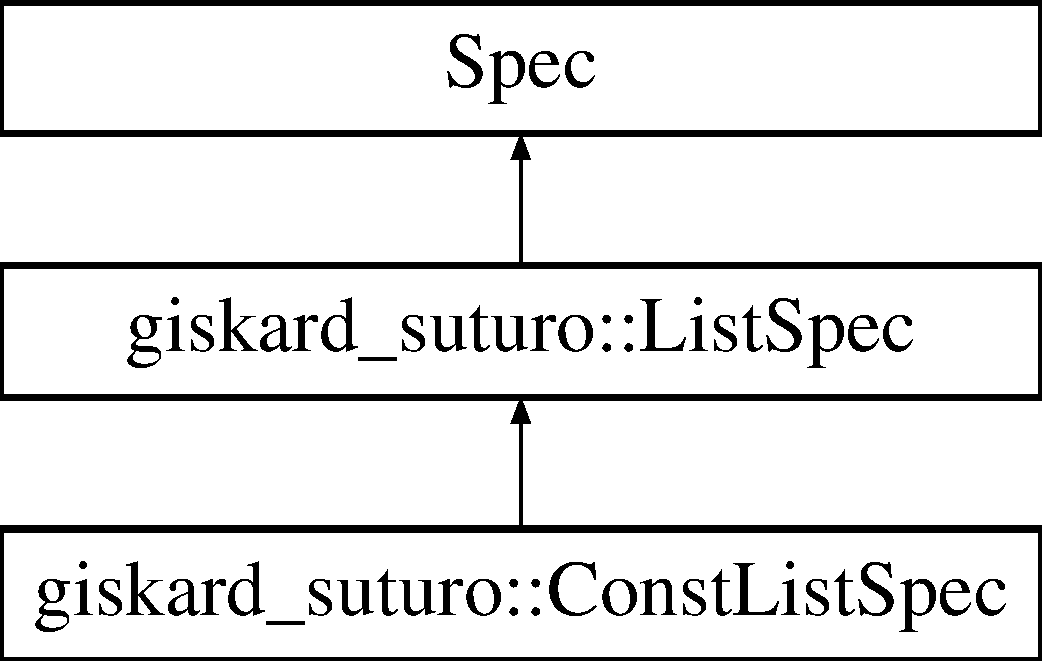
\includegraphics[height=3.000000cm]{classgiskard__suturo_1_1ConstListSpec}
\end{center}
\end{figure}
\subsection*{Public Member Functions}
\begin{DoxyCompactItemize}
\item 
\hypertarget{classgiskard__suturo_1_1ConstListSpec_abb02bc9dc24b253d580deb779896437f}{{\bfseries Const\-List\-Spec} (const std\-::vector$<$ Spec\-Ptr $>$ \&val)}\label{classgiskard__suturo_1_1ConstListSpec_abb02bc9dc24b253d580deb779896437f}

\item 
const Spec\-Ptr \hyperlink{classgiskard__suturo_1_1ConstListSpec_a1373658498d2aa8fe4278daa4950968e}{inner\-Type} () const 
\begin{DoxyCompactList}\small\item\em Returns pointer determining the type of the list's contents. \end{DoxyCompactList}\item 
\hypertarget{classgiskard__suturo_1_1ConstListSpec_aff57dab669937896693aa361ccf8d8d6}{bool {\bfseries equals} (const Spec \&other) const }\label{classgiskard__suturo_1_1ConstListSpec_aff57dab669937896693aa361ccf8d8d6}

\item 
\hypertarget{classgiskard__suturo_1_1ConstListSpec_a30676f4d29567b2aa8109fa10fe80351}{void {\bfseries set\-\_\-value} (const std\-::vector$<$ Spec\-Ptr $>$ \&val)}\label{classgiskard__suturo_1_1ConstListSpec_a30676f4d29567b2aa8109fa10fe80351}

\item 
\hypertarget{classgiskard__suturo_1_1ConstListSpec_ae5530652b0a76365bd7d137f84625434}{std\-::vector$<$ Spec\-Ptr $>$ {\bfseries get\-\_\-value} () const }\label{classgiskard__suturo_1_1ConstListSpec_ae5530652b0a76365bd7d137f84625434}

\item 
\hypertarget{classgiskard__suturo_1_1ConstListSpec_a713a774905b1217fa35d4b9d71152cc0}{void {\bfseries get\-\_\-input\-\_\-specs} (std\-::vector$<$ const Input\-Spec $\ast$ $>$ \&inputs) const }\label{classgiskard__suturo_1_1ConstListSpec_a713a774905b1217fa35d4b9d71152cc0}

\end{DoxyCompactItemize}
\subsection*{Private Attributes}
\begin{DoxyCompactItemize}
\item 
\hypertarget{classgiskard__suturo_1_1ConstListSpec_a137d3d6f4149d636b35dc5727744e04e}{std\-::vector$<$ Spec\-Ptr $>$ {\bfseries value}}\label{classgiskard__suturo_1_1ConstListSpec_a137d3d6f4149d636b35dc5727744e04e}

\end{DoxyCompactItemize}


\subsection{Detailed Description}
List constructor specification. 

\subsection{Member Function Documentation}
\hypertarget{classgiskard__suturo_1_1ConstListSpec_a1373658498d2aa8fe4278daa4950968e}{\index{giskard\-\_\-suturo\-::\-Const\-List\-Spec@{giskard\-\_\-suturo\-::\-Const\-List\-Spec}!inner\-Type@{inner\-Type}}
\index{inner\-Type@{inner\-Type}!giskard_suturo::ConstListSpec@{giskard\-\_\-suturo\-::\-Const\-List\-Spec}}
\subsubsection[{inner\-Type}]{\setlength{\rightskip}{0pt plus 5cm}const Spec\-Ptr giskard\-\_\-suturo\-::\-Const\-List\-Spec\-::inner\-Type (
\begin{DoxyParamCaption}
{}
\end{DoxyParamCaption}
) const\hspace{0.3cm}{\ttfamily [inline]}, {\ttfamily [virtual]}}}\label{classgiskard__suturo_1_1ConstListSpec_a1373658498d2aa8fe4278daa4950968e}


Returns pointer determining the type of the list's contents. 

\begin{DoxyReturn}{Returns}
Type pointer 
\end{DoxyReturn}


Implements \hyperlink{classgiskard__suturo_1_1ListSpec_aba0a625da0d48e702aa723fb6fb3bc7e}{giskard\-\_\-suturo\-::\-List\-Spec}.



The documentation for this class was generated from the following files\-:\begin{DoxyCompactItemize}
\item 
giskard\-\_\-suturo\-\_\-parser/include/giskard\-\_\-suturo\-\_\-parser/specifications.\-h\item 
giskard\-\_\-suturo\-\_\-parser/src/specifications.\-cpp\end{DoxyCompactItemize}

\hypertarget{structgiskard__suturo_1_1GiskardPPParser_1_1Context}{\section{giskard\-\_\-suturo\-:\-:Giskard\-P\-P\-Parser\-:\-:Context Struct Reference}
\label{structgiskard__suturo_1_1GiskardPPParser_1_1Context}\index{giskard\-\_\-suturo\-::\-Giskard\-P\-P\-Parser\-::\-Context@{giskard\-\_\-suturo\-::\-Giskard\-P\-P\-Parser\-::\-Context}}
}


Internal structure used for generating stack traces.  


\subsection*{Public Attributes}
\begin{DoxyCompactItemize}
\item 
\hypertarget{structgiskard__suturo_1_1GiskardPPParser_1_1Context_a33307772788f272707887e92be6e26dd}{S\-It {\bfseries begin}}\label{structgiskard__suturo_1_1GiskardPPParser_1_1Context_a33307772788f272707887e92be6e26dd}

\item 
\hypertarget{structgiskard__suturo_1_1GiskardPPParser_1_1Context_aef04bfba21f8549e278ca6cc69224d8b}{size\-\_\-t {\bfseries line}}\label{structgiskard__suturo_1_1GiskardPPParser_1_1Context_aef04bfba21f8549e278ca6cc69224d8b}

\item 
\hypertarget{structgiskard__suturo_1_1GiskardPPParser_1_1Context_aecc93fdcfcadf0049ab4fdcaac1f12f1}{std\-::string {\bfseries name}}\label{structgiskard__suturo_1_1GiskardPPParser_1_1Context_aecc93fdcfcadf0049ab4fdcaac1f12f1}

\end{DoxyCompactItemize}


\subsection{Detailed Description}
Internal structure used for generating stack traces. 

The documentation for this struct was generated from the following file\-:\begin{DoxyCompactItemize}
\item 
giskard\-\_\-suturo\-\_\-parser/include/giskard\-\_\-suturo\-\_\-parser/parser.\-h\end{DoxyCompactItemize}

\hypertarget{structYAML_1_1convert_3_01suturo__manipulation__msgs_1_1TypedParam_01_4}{\section{Y\-A\-M\-L\-:\-:convert$<$ suturo\-\_\-manipulation\-\_\-msgs\-:\-:Typed\-Param $>$ Struct Template Reference}
\label{structYAML_1_1convert_3_01suturo__manipulation__msgs_1_1TypedParam_01_4}\index{Y\-A\-M\-L\-::convert$<$ suturo\-\_\-manipulation\-\_\-msgs\-::\-Typed\-Param $>$@{Y\-A\-M\-L\-::convert$<$ suturo\-\_\-manipulation\-\_\-msgs\-::\-Typed\-Param $>$}}
}
\subsection*{Static Public Member Functions}
\begin{DoxyCompactItemize}
\item 
\hypertarget{structYAML_1_1convert_3_01suturo__manipulation__msgs_1_1TypedParam_01_4_a7c877e63fa7c84e896a9751e347818c4}{static bool {\bfseries decode} (const Node \&node, suturo\-\_\-manipulation\-\_\-msgs\-::\-Typed\-Param \&rhs)}\label{structYAML_1_1convert_3_01suturo__manipulation__msgs_1_1TypedParam_01_4_a7c877e63fa7c84e896a9751e347818c4}

\end{DoxyCompactItemize}


The documentation for this struct was generated from the following file\-:\begin{DoxyCompactItemize}
\item 
suturo\-\_\-action\-\_\-server/src/client\-\_\-test.\-cpp\end{DoxyCompactItemize}

\hypertarget{structgiskard__suturo_1_1Declaration}{\section{giskard\-\_\-suturo\-:\-:Declaration Struct Reference}
\label{structgiskard__suturo_1_1Declaration}\index{giskard\-\_\-suturo\-::\-Declaration@{giskard\-\_\-suturo\-::\-Declaration}}
}


Structure containing a declaration.  




{\ttfamily \#include $<$parser.\-h$>$}

\subsection*{Public Member Functions}
\begin{DoxyCompactItemize}
\item 
\hypertarget{structgiskard__suturo_1_1Declaration_ac9e40e3addb187fbf764e6bf9e9453a7}{{\bfseries Declaration} (std\-::string \-\_\-name, Spec\-Ptr \-\_\-type)}\label{structgiskard__suturo_1_1Declaration_ac9e40e3addb187fbf764e6bf9e9453a7}

\end{DoxyCompactItemize}
\subsection*{Public Attributes}
\begin{DoxyCompactItemize}
\item 
\hypertarget{structgiskard__suturo_1_1Declaration_a66142005ced1a5b5e8f240fb7c6c1fbd}{std\-::string {\bfseries name}}\label{structgiskard__suturo_1_1Declaration_a66142005ced1a5b5e8f240fb7c6c1fbd}

\item 
\hypertarget{structgiskard__suturo_1_1Declaration_a80f34f240231a669bf8cd2a56d05c0a9}{Spec\-Ptr {\bfseries type}}\label{structgiskard__suturo_1_1Declaration_a80f34f240231a669bf8cd2a56d05c0a9}

\end{DoxyCompactItemize}


\subsection{Detailed Description}
Structure containing a declaration. 

The documentation for this struct was generated from the following file\-:\begin{DoxyCompactItemize}
\item 
giskard\-\_\-suturo\-\_\-parser/include/giskard\-\_\-suturo\-\_\-parser/parser.\-h\end{DoxyCompactItemize}

\hypertarget{classgiskard__suturo_1_1DoubleFunctionCallCache}{\section{giskard\-\_\-suturo\-:\-:Double\-Function\-Call\-Cache Class Reference}
\label{classgiskard__suturo_1_1DoubleFunctionCallCache}\index{giskard\-\_\-suturo\-::\-Double\-Function\-Call\-Cache@{giskard\-\_\-suturo\-::\-Double\-Function\-Call\-Cache}}
}


Function call cache for scalar functions.  




{\ttfamily \#include $<$functions.\-h$>$}

Inheritance diagram for giskard\-\_\-suturo\-:\-:Double\-Function\-Call\-Cache\-:\begin{figure}[H]
\begin{center}
\leavevmode
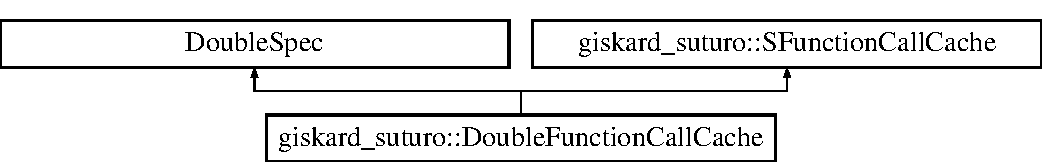
\includegraphics[height=2.000000cm]{classgiskard__suturo_1_1DoubleFunctionCallCache}
\end{center}
\end{figure}
\subsection*{Public Member Functions}
\begin{DoxyCompactItemize}
\item 
\hypertarget{classgiskard__suturo_1_1DoubleFunctionCallCache_a34971a65c735c787f4bf89f6d94837ab}{{\bfseries Double\-Function\-Call\-Cache} (std\-::vector$<$ Spec\-Ptr $>$ \-\_\-arguments, Fn\-Def\-Ptr \-\_\-fn\-Def)}\label{classgiskard__suturo_1_1DoubleFunctionCallCache_a34971a65c735c787f4bf89f6d94837ab}

\item 
\hypertarget{classgiskard__suturo_1_1DoubleFunctionCallCache_a2dba5914aa14674c8772b3256c3ef43e}{virtual bool {\bfseries equals} (const Spec \&other) const }\label{classgiskard__suturo_1_1DoubleFunctionCallCache_a2dba5914aa14674c8772b3256c3ef43e}

\item 
\hypertarget{classgiskard__suturo_1_1DoubleFunctionCallCache_ac0da88d76e96612b38c98eea54835e12}{void {\bfseries get\-\_\-input\-\_\-specs} (std\-::vector$<$ const Input\-Spec $\ast$ $>$ \&inputs) const }\label{classgiskard__suturo_1_1DoubleFunctionCallCache_ac0da88d76e96612b38c98eea54835e12}

\item 
\hypertarget{classgiskard__suturo_1_1DoubleFunctionCallCache_a71ab6c47e9dd1f1143b9e82f315c3f53}{K\-D\-L\-::\-Expression$<$ double $>$\-::Ptr {\bfseries get\-\_\-expression} (const giskard\-\_\-core\-::\-Scope \&scope)}\label{classgiskard__suturo_1_1DoubleFunctionCallCache_a71ab6c47e9dd1f1143b9e82f315c3f53}

\end{DoxyCompactItemize}
\subsection*{Additional Inherited Members}


\subsection{Detailed Description}
Function call cache for scalar functions. 

The documentation for this class was generated from the following file\-:\begin{DoxyCompactItemize}
\item 
giskard\-\_\-suturo\-\_\-parser/include/giskard\-\_\-suturo\-\_\-parser/functions.\-h\end{DoxyCompactItemize}

\hypertarget{structElapsedTimeQuery}{\section{Elapsed\-Time\-Query Struct Reference}
\label{structElapsedTimeQuery}\index{Elapsed\-Time\-Query@{Elapsed\-Time\-Query}}
}


Query assigning the time passed since the start of the controller to an input.  




{\ttfamily \#include $<$Giskard\-Action\-Server.\-h$>$}

Inheritance diagram for Elapsed\-Time\-Query\-:\begin{figure}[H]
\begin{center}
\leavevmode
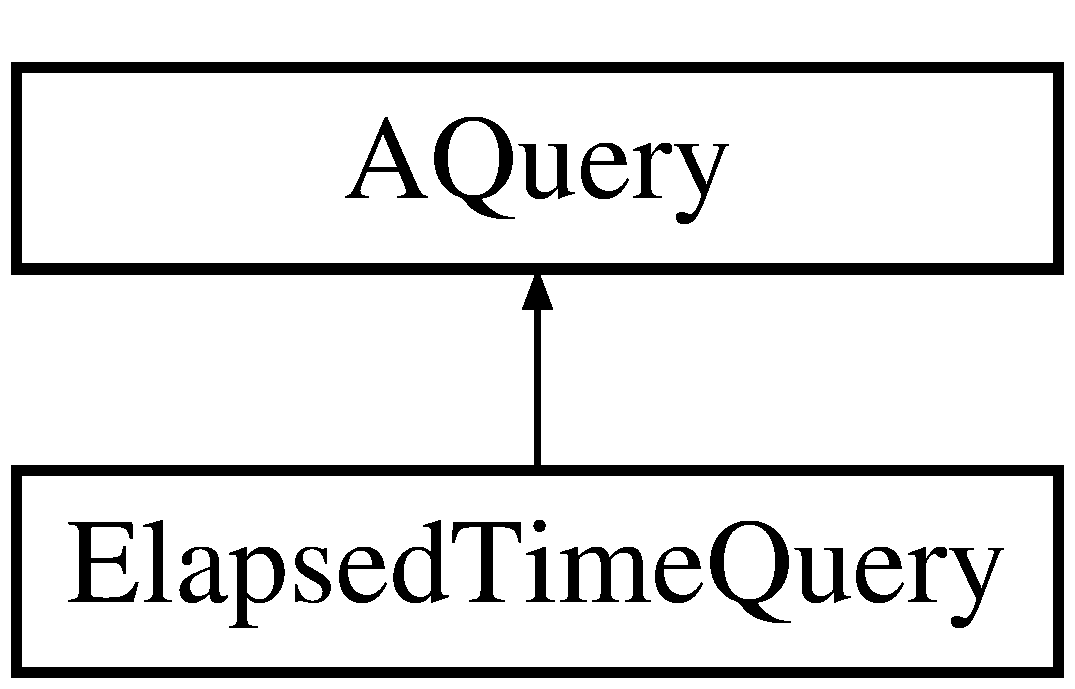
\includegraphics[height=2.000000cm]{structElapsedTimeQuery}
\end{center}
\end{figure}
\subsection*{Public Member Functions}
\begin{DoxyCompactItemize}
\item 
\hypertarget{structElapsedTimeQuery_ae73be34187f2bb1cc78290a7cda92021}{{\bfseries Elapsed\-Time\-Query} (\hyperlink{classGiskardActionServer}{Giskard\-Action\-Server} $\ast$\-\_\-p\-Server, string \-\_\-name)}\label{structElapsedTimeQuery_ae73be34187f2bb1cc78290a7cda92021}

\item 
\hypertarget{structElapsedTimeQuery_a59daf36a1a9d65eb30c43b51f52b6ef7}{bool {\bfseries eval} ()}\label{structElapsedTimeQuery_a59daf36a1a9d65eb30c43b51f52b6ef7}

\end{DoxyCompactItemize}
\subsection*{Private Attributes}
\begin{DoxyCompactItemize}
\item 
const ros\-::\-Time \hyperlink{structElapsedTimeQuery_a4b53ade61743b5e03306d177a09a0dd7}{start}
\end{DoxyCompactItemize}
\subsection*{Additional Inherited Members}


\subsection{Detailed Description}
Query assigning the time passed since the start of the controller to an input. 

\subsection{Member Data Documentation}
\hypertarget{structElapsedTimeQuery_a4b53ade61743b5e03306d177a09a0dd7}{\index{Elapsed\-Time\-Query@{Elapsed\-Time\-Query}!start@{start}}
\index{start@{start}!ElapsedTimeQuery@{Elapsed\-Time\-Query}}
\subsubsection[{start}]{\setlength{\rightskip}{0pt plus 5cm}const ros\-::\-Time Elapsed\-Time\-Query\-::start\hspace{0.3cm}{\ttfamily [private]}}}\label{structElapsedTimeQuery_a4b53ade61743b5e03306d177a09a0dd7}
Time when controller started 

The documentation for this struct was generated from the following file\-:\begin{DoxyCompactItemize}
\item 
suturo\-\_\-action\-\_\-server/include/suturo\-\_\-action\-\_\-server/Giskard\-Action\-Server.\-h\end{DoxyCompactItemize}

\hypertarget{structgiskard__suturo_1_1GiskardLangParser_1_1EOSException}{\section{giskard\-\_\-suturo\-:\-:Giskard\-Lang\-Parser\-:\-:E\-O\-S\-Exception Struct Reference}
\label{structgiskard__suturo_1_1GiskardLangParser_1_1EOSException}\index{giskard\-\_\-suturo\-::\-Giskard\-Lang\-Parser\-::\-E\-O\-S\-Exception@{giskard\-\_\-suturo\-::\-Giskard\-Lang\-Parser\-::\-E\-O\-S\-Exception}}
}
Inheritance diagram for giskard\-\_\-suturo\-:\-:Giskard\-Lang\-Parser\-:\-:E\-O\-S\-Exception\-:\begin{figure}[H]
\begin{center}
\leavevmode
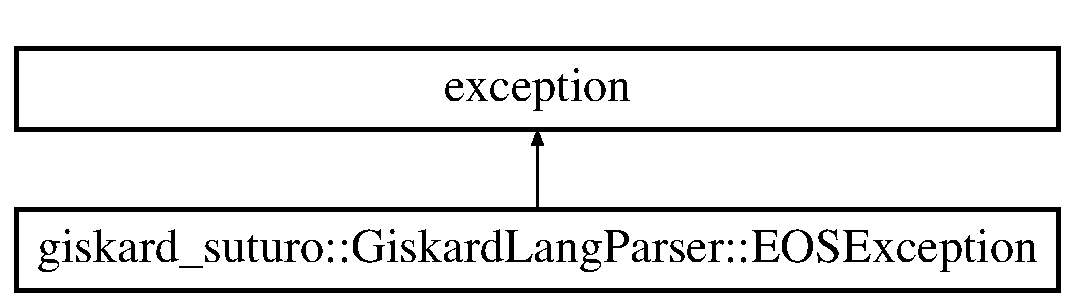
\includegraphics[height=2.000000cm]{structgiskard__suturo_1_1GiskardLangParser_1_1EOSException}
\end{center}
\end{figure}
\subsection*{Public Member Functions}
\begin{DoxyCompactItemize}
\item 
\hypertarget{structgiskard__suturo_1_1GiskardLangParser_1_1EOSException_abcfe54b8cc274217174feefae2ce021c}{const char $\ast$ {\bfseries what} () const noexcept}\label{structgiskard__suturo_1_1GiskardLangParser_1_1EOSException_abcfe54b8cc274217174feefae2ce021c}

\end{DoxyCompactItemize}


The documentation for this struct was generated from the following file\-:\begin{DoxyCompactItemize}
\item 
giskard\-\_\-suturo\-\_\-parser/include/giskard\-\_\-suturo\-\_\-parser/giskard\-\_\-parser.\-hpp\end{DoxyCompactItemize}

\hypertarget{classgiskard__suturo_1_1FrameFunctionCallCache}{\section{giskard\-\_\-suturo\-:\-:Frame\-Function\-Call\-Cache Class Reference}
\label{classgiskard__suturo_1_1FrameFunctionCallCache}\index{giskard\-\_\-suturo\-::\-Frame\-Function\-Call\-Cache@{giskard\-\_\-suturo\-::\-Frame\-Function\-Call\-Cache}}
}


Function call cache for frame functions.  




{\ttfamily \#include $<$functions.\-h$>$}

Inheritance diagram for giskard\-\_\-suturo\-:\-:Frame\-Function\-Call\-Cache\-:\begin{figure}[H]
\begin{center}
\leavevmode
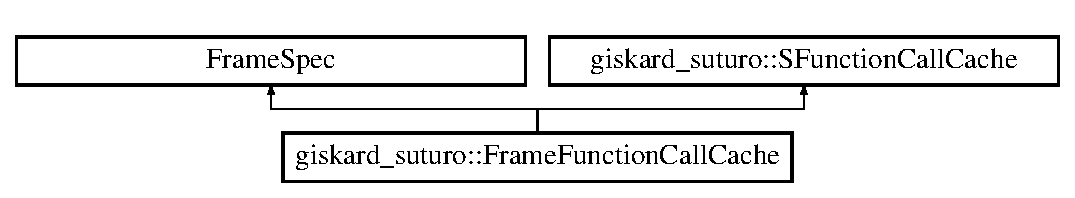
\includegraphics[height=2.000000cm]{classgiskard__suturo_1_1FrameFunctionCallCache}
\end{center}
\end{figure}
\subsection*{Public Member Functions}
\begin{DoxyCompactItemize}
\item 
\hypertarget{classgiskard__suturo_1_1FrameFunctionCallCache_aaf8212b31b7f566c96be7192e2fc5e78}{{\bfseries Frame\-Function\-Call\-Cache} (std\-::vector$<$ Spec\-Ptr $>$ \-\_\-arguments, Fn\-Def\-Ptr \-\_\-fn\-Def)}\label{classgiskard__suturo_1_1FrameFunctionCallCache_aaf8212b31b7f566c96be7192e2fc5e78}

\item 
\hypertarget{classgiskard__suturo_1_1FrameFunctionCallCache_a62f4cc3a3ae7aea67ac9e5f60d85926c}{virtual bool {\bfseries equals} (const Spec \&other) const }\label{classgiskard__suturo_1_1FrameFunctionCallCache_a62f4cc3a3ae7aea67ac9e5f60d85926c}

\item 
\hypertarget{classgiskard__suturo_1_1FrameFunctionCallCache_a10a2a519997b06ed7a35ae44e2540180}{void {\bfseries get\-\_\-input\-\_\-specs} (std\-::vector$<$ const Input\-Spec $\ast$ $>$ \&inputs) const }\label{classgiskard__suturo_1_1FrameFunctionCallCache_a10a2a519997b06ed7a35ae44e2540180}

\item 
\hypertarget{classgiskard__suturo_1_1FrameFunctionCallCache_a953ea6676e6ef0904b014c546c5b1fec}{K\-D\-L\-::\-Expression$<$ K\-D\-L\-::\-Frame $>$\-::Ptr {\bfseries get\-\_\-expression} (const giskard\-\_\-core\-::\-Scope \&scope)}\label{classgiskard__suturo_1_1FrameFunctionCallCache_a953ea6676e6ef0904b014c546c5b1fec}

\end{DoxyCompactItemize}
\subsection*{Additional Inherited Members}


\subsection{Detailed Description}
Function call cache for frame functions. 

The documentation for this class was generated from the following file\-:\begin{DoxyCompactItemize}
\item 
giskard\-\_\-suturo\-\_\-parser/include/giskard\-\_\-suturo\-\_\-parser/functions.\-h\end{DoxyCompactItemize}

\hypertarget{structgiskard__suturo_1_1FunctionCall}{\section{giskard\-\_\-suturo\-:\-:Function\-Call Struct Reference}
\label{structgiskard__suturo_1_1FunctionCall}\index{giskard\-\_\-suturo\-::\-Function\-Call@{giskard\-\_\-suturo\-::\-Function\-Call}}
}


Structure containing data needed for a function call.  




{\ttfamily \#include $<$advanced\-\_\-scope.\-h$>$}

\subsection*{Public Attributes}
\begin{DoxyCompactItemize}
\item 
\hypertarget{structgiskard__suturo_1_1FunctionCall_a38322c530133415cdc18b386e4f3c598}{Fn\-Def\-Ptr {\bfseries function}}\label{structgiskard__suturo_1_1FunctionCall_a38322c530133415cdc18b386e4f3c598}

\item 
\hypertarget{structgiskard__suturo_1_1FunctionCall_a16141e925cddc23ae3397481942acbe9}{std\-::vector$<$ Spec\-Ptr $>$ {\bfseries arguments}}\label{structgiskard__suturo_1_1FunctionCall_a16141e925cddc23ae3397481942acbe9}

\item 
\hypertarget{structgiskard__suturo_1_1FunctionCall_af21b932d20f8129327e184efef65e345}{Spec\-Ptr {\bfseries return\-Reference}}\label{structgiskard__suturo_1_1FunctionCall_af21b932d20f8129327e184efef65e345}

\end{DoxyCompactItemize}


\subsection{Detailed Description}
Structure containing data needed for a function call. 

The documentation for this struct was generated from the following file\-:\begin{DoxyCompactItemize}
\item 
giskard\-\_\-suturo\-\_\-parser/include/giskard\-\_\-suturo\-\_\-parser/advanced\-\_\-scope.\-h\end{DoxyCompactItemize}

\hypertarget{classgiskard__suturo_1_1FunctionDefinition}{\section{giskard\-\_\-suturo\-:\-:Function\-Definition Class Reference}
\label{classgiskard__suturo_1_1FunctionDefinition}\index{giskard\-\_\-suturo\-::\-Function\-Definition@{giskard\-\_\-suturo\-::\-Function\-Definition}}
}


This class models the definition of a function.  




{\ttfamily \#include $<$functions.\-h$>$}

Inheritance diagram for giskard\-\_\-suturo\-:\-:Function\-Definition\-:\begin{figure}[H]
\begin{center}
\leavevmode
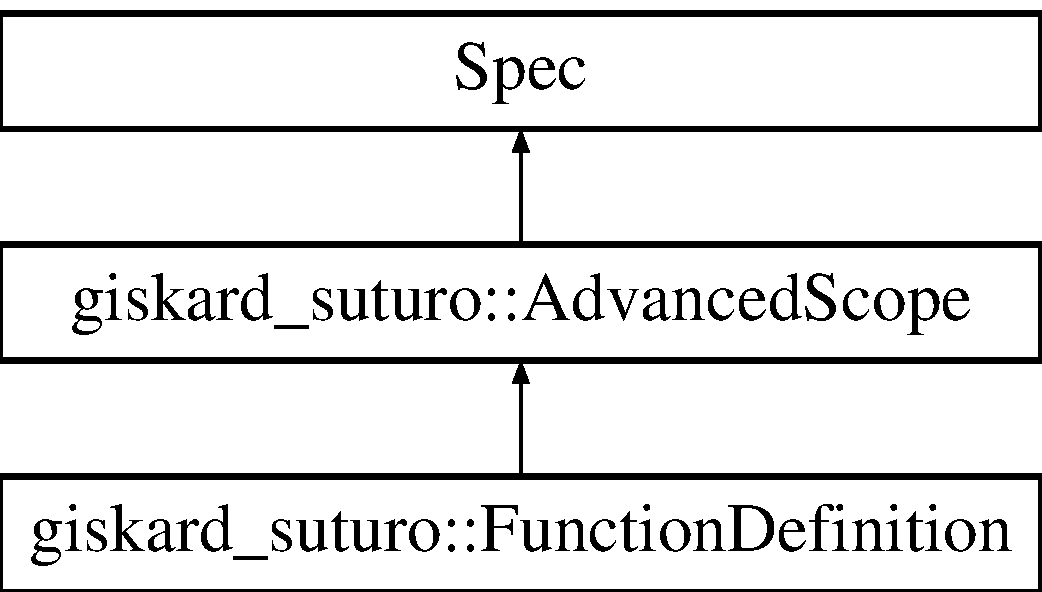
\includegraphics[height=3.000000cm]{classgiskard__suturo_1_1FunctionDefinition}
\end{center}
\end{figure}
\subsection*{Public Member Functions}
\begin{DoxyCompactItemize}
\item 
\hypertarget{classgiskard__suturo_1_1FunctionDefinition_ab054c457aedf56c7ed8dcd85a1bcccb6}{{\bfseries Function\-Definition} (const std\-::string \&\-\_\-name, Advanced\-Scope\-Ptr super\-Scope)}\label{classgiskard__suturo_1_1FunctionDefinition_ab054c457aedf56c7ed8dcd85a1bcccb6}

\item 
void \hyperlink{classgiskard__suturo_1_1FunctionDefinition_ac31bfbad951ac1334c8fe30807132dbe}{add\-Argument} (std\-::string \hyperlink{classgiskard__suturo_1_1FunctionDefinition_ab482fb6e6a9e27255e398c834d1bc813}{name}, Spec\-Ptr spec)
\begin{DoxyCompactList}\small\item\em Adds an argument to the function's signature. \end{DoxyCompactList}\item 
void \hyperlink{classgiskard__suturo_1_1FunctionDefinition_a723dc9bc2d5f964805dadc8af9a8c948}{add\-Spec} (std\-::string \hyperlink{classgiskard__suturo_1_1FunctionDefinition_ab482fb6e6a9e27255e398c834d1bc813}{name}, Spec\-Ptr spec)
\begin{DoxyCompactList}\small\item\em Adds a scope entry. \end{DoxyCompactList}\item 
void \hyperlink{classgiskard__suturo_1_1FunctionDefinition_a384541f47dac5c09c4c7a7e82bdb6820}{add\-Scope} (boost\-::shared\-\_\-ptr$<$ \hyperlink{classgiskard__suturo_1_1AdvancedScope}{Advanced\-Scope} $>$ super\-Scope)
\begin{DoxyCompactList}\small\item\em Adds a super scope. Function definitions can only have one super scope. Trying to add more will cause an exception to be thrown. \end{DoxyCompactList}\item 
void \hyperlink{classgiskard__suturo_1_1FunctionDefinition_a672efdf3e63b221f26ae2d2216d2ec1f}{add\-Scope} (std\-::string alias, boost\-::shared\-\_\-ptr$<$ \hyperlink{classgiskard__suturo_1_1AdvancedScope}{Advanced\-Scope} $>$ super\-Scope)
\begin{DoxyCompactList}\small\item\em Adds a scope. \end{DoxyCompactList}\item 
Spec\-Ptr \hyperlink{classgiskard__suturo_1_1FunctionDefinition_a0132a484566e94d573b180ae12d19093}{create\-Instance} (const std\-::vector$<$ Spec\-Ptr $>$ \&args, Advanced\-Scope\-Ptr \&scope) const 
\begin{DoxyCompactList}\small\item\em Creates an instance of this function with the given parameters in the given scope. \end{DoxyCompactList}\item 
bool \hyperlink{classgiskard__suturo_1_1FunctionDefinition_a26757c1eb352a7aa7c952dd8811dcafa}{check\-Type\-Signature\-Agreement} (const std\-::vector$<$ Spec\-Ptr $>$ args) const 
\begin{DoxyCompactList}\small\item\em Checks whether a list of specifications matches the function's signature. \end{DoxyCompactList}\item 
void \hyperlink{classgiskard__suturo_1_1FunctionDefinition_a788dcb5240b6de0f8a316c70a38be466}{set\-Return\-Spec} (const Spec\-Ptr \&ret\-Spec)
\begin{DoxyCompactList}\small\item\em Sets the specification calculating the return value of the function. \end{DoxyCompactList}\item 
const Spec\-Ptr \hyperlink{classgiskard__suturo_1_1FunctionDefinition_a71a224f73b1bc5357ef4ff225c06c9f8}{get\-Return\-Spec} () const 
\begin{DoxyCompactList}\small\item\em Gets the return specification. \end{DoxyCompactList}\item 
std\-::vector$<$ Spec\-Ptr $>$ \hyperlink{classgiskard__suturo_1_1FunctionDefinition_a688bf1ca593490e3881d97b1e7623f00}{get\-Signature} () const 
\begin{DoxyCompactList}\small\item\em Gets the type trace of the function's signature. \end{DoxyCompactList}\end{DoxyCompactItemize}
\subsection*{Public Attributes}
\begin{DoxyCompactItemize}
\item 
const std\-::string \hyperlink{classgiskard__suturo_1_1FunctionDefinition_ab482fb6e6a9e27255e398c834d1bc813}{name}
\end{DoxyCompactItemize}
\subsection*{Protected Member Functions}
\begin{DoxyCompactItemize}
\item 
bool \hyperlink{classgiskard__suturo_1_1FunctionDefinition_af94fa1fad76a909bb4512af9408fbcaf}{is\-Const\-Spec} (const Spec\-Ptr \&spec\-Ptr) const 
\begin{DoxyCompactList}\small\item\em Internal method for checking whether a specification is constant within this function definition. \end{DoxyCompactList}\end{DoxyCompactItemize}
\subsection*{Private Attributes}
\begin{DoxyCompactItemize}
\item 
Spec\-Ptr \hyperlink{classgiskard__suturo_1_1FunctionDefinition_a17ab4ec5dce5ba78f94917d88b434c29}{return\-Expression}
\item 
std\-::vector$<$ Spec\-Ptr $>$ \hyperlink{classgiskard__suturo_1_1FunctionDefinition_aca5605f42cc4324a219b2fe1d2f53043}{argument\-Specs}
\item 
std\-::vector$<$ std\-::string $>$ \hyperlink{classgiskard__suturo_1_1FunctionDefinition_a6e58c097c4e9e1c97522d394d03ca080}{arguments}
\item 
std\-::unordered\-\_\-map\\*
$<$ std\-::string, bool $>$ \hyperlink{classgiskard__suturo_1_1FunctionDefinition_a824d669129fe7829e3df3f4fd1a3fb9a}{const\-Spec\-Map}
\end{DoxyCompactItemize}
\subsection*{Additional Inherited Members}


\subsection{Detailed Description}
This class models the definition of a function. 

\subsection{Member Function Documentation}
\hypertarget{classgiskard__suturo_1_1FunctionDefinition_ac31bfbad951ac1334c8fe30807132dbe}{\index{giskard\-\_\-suturo\-::\-Function\-Definition@{giskard\-\_\-suturo\-::\-Function\-Definition}!add\-Argument@{add\-Argument}}
\index{add\-Argument@{add\-Argument}!giskard_suturo::FunctionDefinition@{giskard\-\_\-suturo\-::\-Function\-Definition}}
\subsubsection[{add\-Argument}]{\setlength{\rightskip}{0pt plus 5cm}void giskard\-\_\-suturo\-::\-Function\-Definition\-::add\-Argument (
\begin{DoxyParamCaption}
\item[{std\-::string}]{name, }
\item[{Spec\-Ptr}]{spec}
\end{DoxyParamCaption}
)}}\label{classgiskard__suturo_1_1FunctionDefinition_ac31bfbad951ac1334c8fe30807132dbe}


Adds an argument to the function's signature. 


\begin{DoxyParams}[1]{Parameters}
\mbox{\tt in}  & {\em name} & Name of the argument \\
\hline
\mbox{\tt in}  & {\em spec} & Specification of the argument \\
\hline
\end{DoxyParams}
\hypertarget{classgiskard__suturo_1_1FunctionDefinition_a384541f47dac5c09c4c7a7e82bdb6820}{\index{giskard\-\_\-suturo\-::\-Function\-Definition@{giskard\-\_\-suturo\-::\-Function\-Definition}!add\-Scope@{add\-Scope}}
\index{add\-Scope@{add\-Scope}!giskard_suturo::FunctionDefinition@{giskard\-\_\-suturo\-::\-Function\-Definition}}
\subsubsection[{add\-Scope}]{\setlength{\rightskip}{0pt plus 5cm}void giskard\-\_\-suturo\-::\-Function\-Definition\-::add\-Scope (
\begin{DoxyParamCaption}
\item[{boost\-::shared\-\_\-ptr$<$ {\bf Advanced\-Scope} $>$}]{super\-Scope}
\end{DoxyParamCaption}
)}}\label{classgiskard__suturo_1_1FunctionDefinition_a384541f47dac5c09c4c7a7e82bdb6820}


Adds a super scope. Function definitions can only have one super scope. Trying to add more will cause an exception to be thrown. 


\begin{DoxyParams}[1]{Parameters}
\mbox{\tt in}  & {\em super\-Scope} & Super scope to add \\
\hline
\end{DoxyParams}
\hypertarget{classgiskard__suturo_1_1FunctionDefinition_a672efdf3e63b221f26ae2d2216d2ec1f}{\index{giskard\-\_\-suturo\-::\-Function\-Definition@{giskard\-\_\-suturo\-::\-Function\-Definition}!add\-Scope@{add\-Scope}}
\index{add\-Scope@{add\-Scope}!giskard_suturo::FunctionDefinition@{giskard\-\_\-suturo\-::\-Function\-Definition}}
\subsubsection[{add\-Scope}]{\setlength{\rightskip}{0pt plus 5cm}void giskard\-\_\-suturo\-::\-Function\-Definition\-::add\-Scope (
\begin{DoxyParamCaption}
\item[{std\-::string}]{alias, }
\item[{boost\-::shared\-\_\-ptr$<$ {\bf Advanced\-Scope} $>$}]{super\-Scope}
\end{DoxyParamCaption}
)}}\label{classgiskard__suturo_1_1FunctionDefinition_a672efdf3e63b221f26ae2d2216d2ec1f}


Adds a scope. 


\begin{DoxyParams}[1]{Parameters}
\mbox{\tt in}  & {\em alias} & The alias \\
\hline
\mbox{\tt in}  & {\em super\-Scope} & The super scope \\
\hline
\end{DoxyParams}
\hypertarget{classgiskard__suturo_1_1FunctionDefinition_a723dc9bc2d5f964805dadc8af9a8c948}{\index{giskard\-\_\-suturo\-::\-Function\-Definition@{giskard\-\_\-suturo\-::\-Function\-Definition}!add\-Spec@{add\-Spec}}
\index{add\-Spec@{add\-Spec}!giskard_suturo::FunctionDefinition@{giskard\-\_\-suturo\-::\-Function\-Definition}}
\subsubsection[{add\-Spec}]{\setlength{\rightskip}{0pt plus 5cm}void giskard\-\_\-suturo\-::\-Function\-Definition\-::add\-Spec (
\begin{DoxyParamCaption}
\item[{std\-::string}]{name, }
\item[{Spec\-Ptr}]{spec}
\end{DoxyParamCaption}
)\hspace{0.3cm}{\ttfamily [virtual]}}}\label{classgiskard__suturo_1_1FunctionDefinition_a723dc9bc2d5f964805dadc8af9a8c948}


Adds a scope entry. 


\begin{DoxyParams}[1]{Parameters}
\mbox{\tt in}  & {\em name} & Name of the entry \\
\hline
\mbox{\tt in}  & {\em spec} & Specification \\
\hline
\end{DoxyParams}


Reimplemented from \hyperlink{classgiskard__suturo_1_1AdvancedScope_ab3f65ac01f553fabc64c899dde9a4db9}{giskard\-\_\-suturo\-::\-Advanced\-Scope}.

\hypertarget{classgiskard__suturo_1_1FunctionDefinition_a26757c1eb352a7aa7c952dd8811dcafa}{\index{giskard\-\_\-suturo\-::\-Function\-Definition@{giskard\-\_\-suturo\-::\-Function\-Definition}!check\-Type\-Signature\-Agreement@{check\-Type\-Signature\-Agreement}}
\index{check\-Type\-Signature\-Agreement@{check\-Type\-Signature\-Agreement}!giskard_suturo::FunctionDefinition@{giskard\-\_\-suturo\-::\-Function\-Definition}}
\subsubsection[{check\-Type\-Signature\-Agreement}]{\setlength{\rightskip}{0pt plus 5cm}bool giskard\-\_\-suturo\-::\-Function\-Definition\-::check\-Type\-Signature\-Agreement (
\begin{DoxyParamCaption}
\item[{const std\-::vector$<$ Spec\-Ptr $>$}]{args}
\end{DoxyParamCaption}
) const}}\label{classgiskard__suturo_1_1FunctionDefinition_a26757c1eb352a7aa7c952dd8811dcafa}


Checks whether a list of specifications matches the function's signature. 


\begin{DoxyParams}[1]{Parameters}
\mbox{\tt in}  & {\em args} & The specifications to check against\\
\hline
\end{DoxyParams}
\begin{DoxyReturn}{Returns}
True if the check passes, false otherwise. 
\end{DoxyReturn}
\hypertarget{classgiskard__suturo_1_1FunctionDefinition_a0132a484566e94d573b180ae12d19093}{\index{giskard\-\_\-suturo\-::\-Function\-Definition@{giskard\-\_\-suturo\-::\-Function\-Definition}!create\-Instance@{create\-Instance}}
\index{create\-Instance@{create\-Instance}!giskard_suturo::FunctionDefinition@{giskard\-\_\-suturo\-::\-Function\-Definition}}
\subsubsection[{create\-Instance}]{\setlength{\rightskip}{0pt plus 5cm}Spec\-Ptr giskard\-\_\-suturo\-::\-Function\-Definition\-::create\-Instance (
\begin{DoxyParamCaption}
\item[{const std\-::vector$<$ Spec\-Ptr $>$ \&}]{args, }
\item[{Advanced\-Scope\-Ptr \&}]{scope}
\end{DoxyParamCaption}
) const}}\label{classgiskard__suturo_1_1FunctionDefinition_a0132a484566e94d573b180ae12d19093}


Creates an instance of this function with the given parameters in the given scope. 


\begin{DoxyParams}[1]{Parameters}
\mbox{\tt in}  & {\em args} & Arguments for the function call \\
\hline
 & {\em scope} & The scope creating the instance\\
\hline
\end{DoxyParams}
\begin{DoxyReturn}{Returns}
A reference specification linking to the name of the return value of the instance 
\end{DoxyReturn}
\hypertarget{classgiskard__suturo_1_1FunctionDefinition_a71a224f73b1bc5357ef4ff225c06c9f8}{\index{giskard\-\_\-suturo\-::\-Function\-Definition@{giskard\-\_\-suturo\-::\-Function\-Definition}!get\-Return\-Spec@{get\-Return\-Spec}}
\index{get\-Return\-Spec@{get\-Return\-Spec}!giskard_suturo::FunctionDefinition@{giskard\-\_\-suturo\-::\-Function\-Definition}}
\subsubsection[{get\-Return\-Spec}]{\setlength{\rightskip}{0pt plus 5cm}const Spec\-Ptr giskard\-\_\-suturo\-::\-Function\-Definition\-::get\-Return\-Spec (
\begin{DoxyParamCaption}
{}
\end{DoxyParamCaption}
) const\hspace{0.3cm}{\ttfamily [inline]}}}\label{classgiskard__suturo_1_1FunctionDefinition_a71a224f73b1bc5357ef4ff225c06c9f8}


Gets the return specification. 

\begin{DoxyReturn}{Returns}
The return specification. 
\end{DoxyReturn}
\hypertarget{classgiskard__suturo_1_1FunctionDefinition_a688bf1ca593490e3881d97b1e7623f00}{\index{giskard\-\_\-suturo\-::\-Function\-Definition@{giskard\-\_\-suturo\-::\-Function\-Definition}!get\-Signature@{get\-Signature}}
\index{get\-Signature@{get\-Signature}!giskard_suturo::FunctionDefinition@{giskard\-\_\-suturo\-::\-Function\-Definition}}
\subsubsection[{get\-Signature}]{\setlength{\rightskip}{0pt plus 5cm}std\-::vector$<$ Spec\-Ptr $>$ giskard\-\_\-suturo\-::\-Function\-Definition\-::get\-Signature (
\begin{DoxyParamCaption}
{}
\end{DoxyParamCaption}
) const}}\label{classgiskard__suturo_1_1FunctionDefinition_a688bf1ca593490e3881d97b1e7623f00}


Gets the type trace of the function's signature. 

\begin{DoxyReturn}{Returns}
List of types matching the function's signature 
\end{DoxyReturn}
\hypertarget{classgiskard__suturo_1_1FunctionDefinition_af94fa1fad76a909bb4512af9408fbcaf}{\index{giskard\-\_\-suturo\-::\-Function\-Definition@{giskard\-\_\-suturo\-::\-Function\-Definition}!is\-Const\-Spec@{is\-Const\-Spec}}
\index{is\-Const\-Spec@{is\-Const\-Spec}!giskard_suturo::FunctionDefinition@{giskard\-\_\-suturo\-::\-Function\-Definition}}
\subsubsection[{is\-Const\-Spec}]{\setlength{\rightskip}{0pt plus 5cm}bool giskard\-\_\-suturo\-::\-Function\-Definition\-::is\-Const\-Spec (
\begin{DoxyParamCaption}
\item[{const Spec\-Ptr \&}]{spec\-Ptr}
\end{DoxyParamCaption}
) const\hspace{0.3cm}{\ttfamily [protected]}}}\label{classgiskard__suturo_1_1FunctionDefinition_af94fa1fad76a909bb4512af9408fbcaf}


Internal method for checking whether a specification is constant within this function definition. 


\begin{DoxyParams}[1]{Parameters}
\mbox{\tt in}  & {\em spec\-Ptr} & Specification to check.\\
\hline
\end{DoxyParams}
\begin{DoxyReturn}{Returns}
True if specification is constant, False otherwise. 
\end{DoxyReturn}
\hypertarget{classgiskard__suturo_1_1FunctionDefinition_a788dcb5240b6de0f8a316c70a38be466}{\index{giskard\-\_\-suturo\-::\-Function\-Definition@{giskard\-\_\-suturo\-::\-Function\-Definition}!set\-Return\-Spec@{set\-Return\-Spec}}
\index{set\-Return\-Spec@{set\-Return\-Spec}!giskard_suturo::FunctionDefinition@{giskard\-\_\-suturo\-::\-Function\-Definition}}
\subsubsection[{set\-Return\-Spec}]{\setlength{\rightskip}{0pt plus 5cm}void giskard\-\_\-suturo\-::\-Function\-Definition\-::set\-Return\-Spec (
\begin{DoxyParamCaption}
\item[{const Spec\-Ptr \&}]{ret\-Spec}
\end{DoxyParamCaption}
)\hspace{0.3cm}{\ttfamily [inline]}}}\label{classgiskard__suturo_1_1FunctionDefinition_a788dcb5240b6de0f8a316c70a38be466}


Sets the specification calculating the return value of the function. 


\begin{DoxyParams}[1]{Parameters}
\mbox{\tt in}  & {\em ret\-Spec} & The return specification \\
\hline
\end{DoxyParams}


\subsection{Member Data Documentation}
\hypertarget{classgiskard__suturo_1_1FunctionDefinition_a6e58c097c4e9e1c97522d394d03ca080}{\index{giskard\-\_\-suturo\-::\-Function\-Definition@{giskard\-\_\-suturo\-::\-Function\-Definition}!arguments@{arguments}}
\index{arguments@{arguments}!giskard_suturo::FunctionDefinition@{giskard\-\_\-suturo\-::\-Function\-Definition}}
\subsubsection[{arguments}]{\setlength{\rightskip}{0pt plus 5cm}std\-::vector$<$std\-::string$>$ giskard\-\_\-suturo\-::\-Function\-Definition\-::arguments\hspace{0.3cm}{\ttfamily [private]}}}\label{classgiskard__suturo_1_1FunctionDefinition_a6e58c097c4e9e1c97522d394d03ca080}
Names of the function's arguments \hypertarget{classgiskard__suturo_1_1FunctionDefinition_aca5605f42cc4324a219b2fe1d2f53043}{\index{giskard\-\_\-suturo\-::\-Function\-Definition@{giskard\-\_\-suturo\-::\-Function\-Definition}!argument\-Specs@{argument\-Specs}}
\index{argument\-Specs@{argument\-Specs}!giskard_suturo::FunctionDefinition@{giskard\-\_\-suturo\-::\-Function\-Definition}}
\subsubsection[{argument\-Specs}]{\setlength{\rightskip}{0pt plus 5cm}std\-::vector$<$Spec\-Ptr$>$ giskard\-\_\-suturo\-::\-Function\-Definition\-::argument\-Specs\hspace{0.3cm}{\ttfamily [private]}}}\label{classgiskard__suturo_1_1FunctionDefinition_aca5605f42cc4324a219b2fe1d2f53043}
Placeholder specifications for arguments \hypertarget{classgiskard__suturo_1_1FunctionDefinition_a824d669129fe7829e3df3f4fd1a3fb9a}{\index{giskard\-\_\-suturo\-::\-Function\-Definition@{giskard\-\_\-suturo\-::\-Function\-Definition}!const\-Spec\-Map@{const\-Spec\-Map}}
\index{const\-Spec\-Map@{const\-Spec\-Map}!giskard_suturo::FunctionDefinition@{giskard\-\_\-suturo\-::\-Function\-Definition}}
\subsubsection[{const\-Spec\-Map}]{\setlength{\rightskip}{0pt plus 5cm}std\-::unordered\-\_\-map$<$std\-::string, bool$>$ giskard\-\_\-suturo\-::\-Function\-Definition\-::const\-Spec\-Map\hspace{0.3cm}{\ttfamily [private]}}}\label{classgiskard__suturo_1_1FunctionDefinition_a824d669129fe7829e3df3f4fd1a3fb9a}
Map caching whether specifications are constant \hypertarget{classgiskard__suturo_1_1FunctionDefinition_ab482fb6e6a9e27255e398c834d1bc813}{\index{giskard\-\_\-suturo\-::\-Function\-Definition@{giskard\-\_\-suturo\-::\-Function\-Definition}!name@{name}}
\index{name@{name}!giskard_suturo::FunctionDefinition@{giskard\-\_\-suturo\-::\-Function\-Definition}}
\subsubsection[{name}]{\setlength{\rightskip}{0pt plus 5cm}const std\-::string giskard\-\_\-suturo\-::\-Function\-Definition\-::name}}\label{classgiskard__suturo_1_1FunctionDefinition_ab482fb6e6a9e27255e398c834d1bc813}
Name of the defined function \hypertarget{classgiskard__suturo_1_1FunctionDefinition_a17ab4ec5dce5ba78f94917d88b434c29}{\index{giskard\-\_\-suturo\-::\-Function\-Definition@{giskard\-\_\-suturo\-::\-Function\-Definition}!return\-Expression@{return\-Expression}}
\index{return\-Expression@{return\-Expression}!giskard_suturo::FunctionDefinition@{giskard\-\_\-suturo\-::\-Function\-Definition}}
\subsubsection[{return\-Expression}]{\setlength{\rightskip}{0pt plus 5cm}Spec\-Ptr giskard\-\_\-suturo\-::\-Function\-Definition\-::return\-Expression\hspace{0.3cm}{\ttfamily [private]}}}\label{classgiskard__suturo_1_1FunctionDefinition_a17ab4ec5dce5ba78f94917d88b434c29}
Specification of this function's return value 

The documentation for this class was generated from the following files\-:\begin{DoxyCompactItemize}
\item 
giskard\-\_\-suturo\-\_\-parser/include/giskard\-\_\-suturo\-\_\-parser/functions.\-h\item 
giskard\-\_\-suturo\-\_\-parser/src/functions.\-cpp\end{DoxyCompactItemize}

\hypertarget{classGiskardActionServer}{\section{Giskard\-Action\-Server Class Reference}
\label{classGiskardActionServer}\index{Giskard\-Action\-Server@{Giskard\-Action\-Server}}
}


Class for giskard action server. Sets up action server, threads and callbacks.  




{\ttfamily \#include $<$Giskard\-Action\-Server.\-h$>$}

\subsection*{Classes}
\begin{DoxyCompactItemize}
\item 
struct \hyperlink{structGiskardActionServer_1_1gripperController}{gripper\-Controller}
\begin{DoxyCompactList}\small\item\em Internal structure to manage a gripper controller. \end{DoxyCompactList}\item 
struct \hyperlink{structGiskardActionServer_1_1posController}{pos\-Controller}
\begin{DoxyCompactList}\small\item\em Internal structure to manage a position controller. \end{DoxyCompactList}\end{DoxyCompactItemize}
\subsection*{Public Member Functions}
\begin{DoxyCompactItemize}
\item 
\hyperlink{classGiskardActionServer_a8a7027c7e6c35a2d0bb39146ea8233fd}{Giskard\-Action\-Server} (string \-\_\-name)
\begin{DoxyCompactList}\small\item\em Constructor for giskard action server. \end{DoxyCompactList}\item 
virtual void \hyperlink{classGiskardActionServer_aed9b983c543c6f45d1adb023d4ae6e6f}{set\-Goal} (const suturo\-\_\-manipulation\-\_\-msgs\-::\-Move\-Robot\-Goal\-Const\-Ptr \&goal)
\begin{DoxyCompactList}\small\item\em Goal callback for the action server. \end{DoxyCompactList}\item 
virtual void \hyperlink{classGiskardActionServer_ad1b3fb4f09d818b2751d8ec760295149}{load\-Config} (Y\-A\-M\-L\-::\-Node config)
\begin{DoxyCompactList}\small\item\em Configures the action server using a yaml configuration. \end{DoxyCompactList}\item 
void \hyperlink{classGiskardActionServer_ac81b9f53586562358dac417f4ef1df33}{update\-Joint\-State} (const sensor\-\_\-msgs\-::\-Joint\-State\-::\-Const\-Ptr \&joint\-State\-Msg)
\begin{DoxyCompactList}\small\item\em Callback function for receiving joint states. \end{DoxyCompactList}\item 
void \hyperlink{classGiskardActionServer_ad435a52f4d06c69459db72efc1db3662}{update\-Controller} (const sensor\-\_\-msgs\-::\-Joint\-State joint\-State)
\begin{DoxyCompactList}\small\item\em Performs one controller update cycle. \end{DoxyCompactList}\item 
bool \hyperlink{classGiskardActionServer_ab71dfdc1a4c04038b8a769859243d82a}{decode\-Double} (const string \&\hyperlink{classGiskardActionServer_ae1d480bfeed0f97334d25e1dfc868e67}{name}, string value)
\begin{DoxyCompactList}\small\item\em Decodes a scalar parameter from a string and writes it to the state vector. \end{DoxyCompactList}\item 
bool \hyperlink{classGiskardActionServer_a60aebb66785577c5a106de74f6a5c55a}{decode\-Double} (const string \&\hyperlink{classGiskardActionServer_ae1d480bfeed0f97334d25e1dfc868e67}{name}, double value)
\begin{DoxyCompactList}\small\item\em Assigns a scalar parameter to the state vector. \end{DoxyCompactList}\item 
bool \hyperlink{classGiskardActionServer_ae821164a4a9ab651d1243ecace70e7e2}{decode\-Vector} (const string \&\hyperlink{classGiskardActionServer_ae1d480bfeed0f97334d25e1dfc868e67}{name}, string vector)
\begin{DoxyCompactList}\small\item\em Decodes a vector parameter from a string and writes it to the state vector. \end{DoxyCompactList}\item 
bool \hyperlink{classGiskardActionServer_adac7573c728e9e1509b3add22d580ba4}{decode\-Vector} (const string \&\hyperlink{classGiskardActionServer_ae1d480bfeed0f97334d25e1dfc868e67}{name}, Eigen\-::\-Vector3d vector)
\begin{DoxyCompactList}\small\item\em Assigns a vector parameter to the state vector. \end{DoxyCompactList}\item 
bool \hyperlink{classGiskardActionServer_ab1656dc16797cdf15607a42e59435c5b}{decode\-Transform} (const string \&\hyperlink{classGiskardActionServer_ae1d480bfeed0f97334d25e1dfc868e67}{name}, string transform)
\begin{DoxyCompactList}\small\item\em Decodes a transform parameter from a string and writes it to the state vector. \end{DoxyCompactList}\item 
bool \hyperlink{classGiskardActionServer_afd265e6b6c0af3afb6e147b4ee2fe0ff}{decode\-Transform} (const string \&\hyperlink{classGiskardActionServer_ae1d480bfeed0f97334d25e1dfc868e67}{name}, tf\-::\-Transform transform)
\begin{DoxyCompactList}\small\item\em Assigns a transform parameter to the state vector. \end{DoxyCompactList}\end{DoxyCompactItemize}
\subsection*{Protected Attributes}
\begin{DoxyCompactItemize}
\item 
int \hyperlink{classGiskardActionServer_a027ef896e1d60656dc32b7fd827e00c1}{n\-W\-S\-R}
\item 
bool \hyperlink{classGiskardActionServer_acc7002280c576e183f1fc07a7450918e}{terminate\-Execution}
\item 
const string \hyperlink{classGiskardActionServer_ae1d480bfeed0f97334d25e1dfc868e67}{name}
\item 
ros\-::\-Node\-Handle \hyperlink{classGiskardActionServer_a9ff54b2b5811ca6a48b5147a3799697a}{nh}
\item 
actionlib\-::\-Simple\-Action\-Server\\*
$<$ suturo\-\_\-manipulation\-\_\-msgs\-::\-Move\-Robot\-Action $>$ \hyperlink{classGiskardActionServer_aec1639ae446055aff03685e3a3b0bda2}{server}
\item 
giskard\-\_\-core\-::\-Q\-P\-Controller \hyperlink{classGiskardActionServer_a72419de3a5237d2ee09ad92f1ed81da1}{controller}
\item 
Eigen\-::\-Vector\-Xd \hyperlink{classGiskardActionServer_ae79dc838a2d884755866e29d9c02dd77}{state}
\item 
map$<$ std\-::string, ros\-::\-Publisher $>$ \hyperlink{classGiskardActionServer_a4ea7edab163168d8c747f7d2e67b2f67}{vel\-Controllers}
\item 
unordered\-\_\-map$<$ string, \\*
\hyperlink{structGiskardActionServer_1_1posController}{pos\-Controller} $>$ \hyperlink{classGiskardActionServer_a972ee6ac1c1295b7c183cfea96ee4db1}{pos\-Controllers}
\item 
unordered\-\_\-map$<$ string, \\*
\hyperlink{structGiskardActionServer_1_1gripperController}{gripper\-Controller} $>$ \hyperlink{classGiskardActionServer_a20e66f4df22818fd6db1a78b4f9db129}{gripper\-Controllers}
\item 
unordered\-\_\-set$<$ string $>$ \hyperlink{classGiskardActionServer_af4c11bee852dc54f821c4aabbeec5d7c}{joint\-Set}
\item 
vector$<$ boost\-::shared\-\_\-ptr\\*
$<$ \hyperlink{structAQuery}{A\-Query} $>$ $>$ \hyperlink{classGiskardActionServer_ae8224875f2c3e1cba7f38a05c2d8985a}{queries}
\item 
map$<$ string, double $>$ \hyperlink{classGiskardActionServer_a965e4f058e16f29b8a6516d7fd6d45ad}{last\-Command}
\item 
map$<$ string, double $>$ \hyperlink{classGiskardActionServer_a02213acb96763c0283668a519903e440}{last\-Controllable\-Pos}
\item 
ros\-::\-Time \hyperlink{classGiskardActionServer_a549f8c868afd0fff8383fbbe512e4bfa}{last\-Update}
\item 
string \hyperlink{classGiskardActionServer_ab1ff77a2e75bc70378c6e763745593d1}{vis\-Ref\-Frame\-Name}
\end{DoxyCompactItemize}
\subsection*{Private Types}
\begin{DoxyCompactItemize}
\item 
enum \hyperlink{classGiskardActionServer_a3dcd42d3ccb136a49377b68bcdf21078}{Vis\-Types} \-: int \{ {\bfseries v\-Point}, 
{\bfseries v\-Vector}, 
{\bfseries v\-Frame}
 \}
\begin{DoxyCompactList}\small\item\em Enumeration for visualization types. \end{DoxyCompactList}\item 
typedef std\-::pair\\*
$<$ K\-D\-L\-::\-Expression$<$ K\-D\-L\-::\-Vector $>$\\*
\-::Ptr, K\-D\-L\-::\-Expression\\*
$<$ K\-D\-L\-::\-Vector $>$\-::Ptr $>$ \hyperlink{classGiskardActionServer_a49b67ed22398144efcae8cf2d6596f9e}{T\-Vec\-Pair}
\end{DoxyCompactItemize}
\subsection*{Private Member Functions}
\begin{DoxyCompactItemize}
\item 
void \hyperlink{classGiskardActionServer_a4164a1043930f6575d011e3fb7bbb207}{generate\-Visuals\-From\-Scope} (const giskard\-\_\-core\-::\-Scope \&scope)
\begin{DoxyCompactList}\small\item\em Parses controller scope for values to visualize. \end{DoxyCompactList}\end{DoxyCompactItemize}
\subsection*{Private Attributes}
\begin{DoxyCompactItemize}
\item 
mutex \hyperlink{classGiskardActionServer_ac77cdbd8c3b81397c4be868e6711a458}{js\-Mutex}
\item 
bool \hyperlink{classGiskardActionServer_a6af586abe01f748597efea84d3d52e21}{new\-J\-S}
\item 
sensor\-\_\-msgs\-::\-Joint\-State \hyperlink{classGiskardActionServer_a06b9a0bfdf889fd886b4a10c6e0f7fe1}{current\-J\-S}
\item 
double \hyperlink{classGiskardActionServer_aca0c0257a6df8d3563fbdfdc39da1361}{d\-T}
\item 
tf\-::\-Transform\-Listener \hyperlink{classGiskardActionServer_ae7deb327e757759d21614df5adbc42f3}{tf\-Listener}
\item 
double \hyperlink{classGiskardActionServer_a17640817711388e121902779b66a3657}{last\-Feedback}
\item 
ros\-::\-Subscriber \hyperlink{classGiskardActionServer_a4197a9f1da3c9832d4bf7786bffa82ff}{js\-Sub}
\item 
bool \hyperlink{classGiskardActionServer_a46b468b15e97c46911fccfccf960ea76}{controller\-Initialized}
\item 
K\-D\-L\-::\-Expression$<$ double $>$\-::Ptr \hyperlink{classGiskardActionServer_ae68ed4306e57da20d00e80bf38f2e4f1}{feedback\-Expr}
\item 
unordered\-\_\-map$<$ string, \\*
K\-D\-L\-::\-Expression$<$ double $>$\-::Ptr $>$ \hyperlink{classGiskardActionServer_ae04063c56a2103232e3aa88283897666}{vis\-Scalars}
\item 
unordered\-\_\-map$<$ string, \\*
K\-D\-L\-::\-Expression$<$ K\-D\-L\-::\-Vector $>$\\*
\-::Ptr $>$ \hyperlink{classGiskardActionServer_a1094414df8bbfbcf469c88877f46d019}{vis\-Points}
\item 
unordered\-\_\-map$<$ string, \hyperlink{classGiskardActionServer_a49b67ed22398144efcae8cf2d6596f9e}{T\-Vec\-Pair} $>$ \hyperlink{classGiskardActionServer_abdad3a9c717ec286399323b152a8e64d}{vis\-Vectors}
\item 
unordered\-\_\-map$<$ string, \\*
K\-D\-L\-::\-Expression$<$ K\-D\-L\-::\-Frame $>$\\*
\-::Ptr $>$ \hyperlink{classGiskardActionServer_a018f9bc81967e035deb6cec695893dbc}{vis\-Frames}
\item 
ros\-::\-Publisher \hyperlink{classGiskardActionServer_a127b4e7740905cceb5a1ed2affd7fed3}{js\-Cmd\-Pub}
\item 
ros\-::\-Publisher \hyperlink{classGiskardActionServer_ac3e0344ceea38b8113c364b34c2353b2}{pos\-Error\-Pub}
\item 
\hypertarget{classGiskardActionServer_aed767b9547c953f6861a363925a41d88}{ros\-::\-Publisher {\bfseries vel\-Error\-Pub}}\label{classGiskardActionServer_aed767b9547c953f6861a363925a41d88}

\item 
ros\-::\-Publisher \hyperlink{classGiskardActionServer_ad5faa562d8e3e2ea964effb5df90775b}{vis\-Pub}
\item 
\hypertarget{classGiskardActionServer_a6759ab8fd7b1bb1ed5b8341801d483a5}{ros\-::\-Publisher {\bfseries vis\-Scalar\-Pub}}\label{classGiskardActionServer_a6759ab8fd7b1bb1ed5b8341801d483a5}

\item 
\hyperlink{classVisualizationManager}{Visualization\-Manager} \hyperlink{classGiskardActionServer_a4aca89815a5d0cb84475773401613365}{vis\-Manager}
\item 
\hyperlink{classCollisionScene}{Collision\-Scene} \hyperlink{classGiskardActionServer_a9092b32b81ae2e3c13ab6f5632e716a1}{collision\-Scene}
\item 
\hyperlink{classMutexMap}{Collision\-Scene\-::\-Query\-Map} \hyperlink{classGiskardActionServer_a6dc2df6171c07b6c15e20e91533b0430}{coll\-Query\-Map}
\item 
suturo\-\_\-manipulation\-\_\-msgs\-::\-Move\-Robot\-Feedback \hyperlink{classGiskardActionServer_aaa0e1708f9a1af19c33986f0504e7f34}{feedback}
\item 
suturo\-\_\-manipulation\-\_\-msgs\-::\-Move\-Robot\-Result \hyperlink{classGiskardActionServer_a62a22a3a61a61b36a2b4c0d5f6ed1e70}{result}
\end{DoxyCompactItemize}


\subsection{Detailed Description}
Class for giskard action server. Sets up action server, threads and callbacks. 

\subsection{Member Typedef Documentation}
\hypertarget{classGiskardActionServer_a49b67ed22398144efcae8cf2d6596f9e}{\index{Giskard\-Action\-Server@{Giskard\-Action\-Server}!T\-Vec\-Pair@{T\-Vec\-Pair}}
\index{T\-Vec\-Pair@{T\-Vec\-Pair}!GiskardActionServer@{Giskard\-Action\-Server}}
\subsubsection[{T\-Vec\-Pair}]{\setlength{\rightskip}{0pt plus 5cm}typedef std\-::pair$<$K\-D\-L\-::\-Expression$<$K\-D\-L\-::\-Vector$>$\-::Ptr, K\-D\-L\-::\-Expression$<$K\-D\-L\-::\-Vector$>$\-::Ptr$>$ {\bf Giskard\-Action\-Server\-::\-T\-Vec\-Pair}\hspace{0.3cm}{\ttfamily [private]}}}\label{classGiskardActionServer_a49b67ed22398144efcae8cf2d6596f9e}
Type definition for vector visualization. 

\subsection{Constructor \& Destructor Documentation}
\hypertarget{classGiskardActionServer_a8a7027c7e6c35a2d0bb39146ea8233fd}{\index{Giskard\-Action\-Server@{Giskard\-Action\-Server}!Giskard\-Action\-Server@{Giskard\-Action\-Server}}
\index{Giskard\-Action\-Server@{Giskard\-Action\-Server}!GiskardActionServer@{Giskard\-Action\-Server}}
\subsubsection[{Giskard\-Action\-Server}]{\setlength{\rightskip}{0pt plus 5cm}Giskard\-Action\-Server\-::\-Giskard\-Action\-Server (
\begin{DoxyParamCaption}
\item[{string}]{\-\_\-name}
\end{DoxyParamCaption}
)}}\label{classGiskardActionServer_a8a7027c7e6c35a2d0bb39146ea8233fd}


Constructor for giskard action server. 

During construction, an actionlib action server is created and command and visualization topics are advertised. Additional configuration information is read from the parameter $\sim$config on the parameter server.


\begin{DoxyParams}[1]{Parameters}
\mbox{\tt in}  & {\em \-\_\-name} & The name that the actionlib action server will be created with \\
\hline
\end{DoxyParams}


\subsection{Member Function Documentation}
\hypertarget{classGiskardActionServer_ab71dfdc1a4c04038b8a769859243d82a}{\index{Giskard\-Action\-Server@{Giskard\-Action\-Server}!decode\-Double@{decode\-Double}}
\index{decode\-Double@{decode\-Double}!GiskardActionServer@{Giskard\-Action\-Server}}
\subsubsection[{decode\-Double}]{\setlength{\rightskip}{0pt plus 5cm}bool Giskard\-Action\-Server\-::decode\-Double (
\begin{DoxyParamCaption}
\item[{const string \&}]{name, }
\item[{string}]{value}
\end{DoxyParamCaption}
)}}\label{classGiskardActionServer_ab71dfdc1a4c04038b8a769859243d82a}


Decodes a scalar parameter from a string and writes it to the state vector. 


\begin{DoxyParams}[1]{Parameters}
\mbox{\tt in}  & {\em name} & Name of the corresponding input in the current controller \\
\hline
\mbox{\tt in}  & {\em value} & Scalar encoded as string \\
\hline
\end{DoxyParams}
\begin{DoxyReturn}{Returns}
Success of decoding and value assignment. 
\end{DoxyReturn}
\hypertarget{classGiskardActionServer_a60aebb66785577c5a106de74f6a5c55a}{\index{Giskard\-Action\-Server@{Giskard\-Action\-Server}!decode\-Double@{decode\-Double}}
\index{decode\-Double@{decode\-Double}!GiskardActionServer@{Giskard\-Action\-Server}}
\subsubsection[{decode\-Double}]{\setlength{\rightskip}{0pt plus 5cm}bool Giskard\-Action\-Server\-::decode\-Double (
\begin{DoxyParamCaption}
\item[{const string \&}]{name, }
\item[{double}]{value}
\end{DoxyParamCaption}
)}}\label{classGiskardActionServer_a60aebb66785577c5a106de74f6a5c55a}


Assigns a scalar parameter to the state vector. 


\begin{DoxyParams}[1]{Parameters}
\mbox{\tt in}  & {\em name} & Name of the corresponding input in the current controller \\
\hline
\mbox{\tt in}  & {\em value} & Scalar \\
\hline
\end{DoxyParams}
\begin{DoxyReturn}{Returns}
Success of value assignment. 
\end{DoxyReturn}
\hypertarget{classGiskardActionServer_ab1656dc16797cdf15607a42e59435c5b}{\index{Giskard\-Action\-Server@{Giskard\-Action\-Server}!decode\-Transform@{decode\-Transform}}
\index{decode\-Transform@{decode\-Transform}!GiskardActionServer@{Giskard\-Action\-Server}}
\subsubsection[{decode\-Transform}]{\setlength{\rightskip}{0pt plus 5cm}bool Giskard\-Action\-Server\-::decode\-Transform (
\begin{DoxyParamCaption}
\item[{const string \&}]{name, }
\item[{string}]{transform}
\end{DoxyParamCaption}
)}}\label{classGiskardActionServer_ab1656dc16797cdf15607a42e59435c5b}


Decodes a transform parameter from a string and writes it to the state vector. 


\begin{DoxyParams}[1]{Parameters}
\mbox{\tt in}  & {\em name} & Name of the corresponding input in the current controller \\
\hline
\mbox{\tt in}  & {\em vector} & Transform encoded as string\-: \char`\"{}\-X Y Z A\-X A\-Y A\-Z Angle\char`\"{} \\
\hline
\end{DoxyParams}
\begin{DoxyReturn}{Returns}
Success of decoding and value assignment. 
\end{DoxyReturn}
\hypertarget{classGiskardActionServer_afd265e6b6c0af3afb6e147b4ee2fe0ff}{\index{Giskard\-Action\-Server@{Giskard\-Action\-Server}!decode\-Transform@{decode\-Transform}}
\index{decode\-Transform@{decode\-Transform}!GiskardActionServer@{Giskard\-Action\-Server}}
\subsubsection[{decode\-Transform}]{\setlength{\rightskip}{0pt plus 5cm}bool Giskard\-Action\-Server\-::decode\-Transform (
\begin{DoxyParamCaption}
\item[{const string \&}]{name, }
\item[{tf\-::\-Transform}]{transform}
\end{DoxyParamCaption}
)}}\label{classGiskardActionServer_afd265e6b6c0af3afb6e147b4ee2fe0ff}


Assigns a transform parameter to the state vector. 


\begin{DoxyParams}[1]{Parameters}
\mbox{\tt in}  & {\em name} & Name of the corresponding input in the current controller \\
\hline
\mbox{\tt in}  & {\em vector} & Transform \\
\hline
\end{DoxyParams}
\begin{DoxyReturn}{Returns}
Success of value assignment. 
\end{DoxyReturn}
\hypertarget{classGiskardActionServer_ae821164a4a9ab651d1243ecace70e7e2}{\index{Giskard\-Action\-Server@{Giskard\-Action\-Server}!decode\-Vector@{decode\-Vector}}
\index{decode\-Vector@{decode\-Vector}!GiskardActionServer@{Giskard\-Action\-Server}}
\subsubsection[{decode\-Vector}]{\setlength{\rightskip}{0pt plus 5cm}bool Giskard\-Action\-Server\-::decode\-Vector (
\begin{DoxyParamCaption}
\item[{const string \&}]{name, }
\item[{string}]{vector}
\end{DoxyParamCaption}
)}}\label{classGiskardActionServer_ae821164a4a9ab651d1243ecace70e7e2}


Decodes a vector parameter from a string and writes it to the state vector. 


\begin{DoxyParams}[1]{Parameters}
\mbox{\tt in}  & {\em name} & Name of the corresponding input in the current controller \\
\hline
\mbox{\tt in}  & {\em vector} & Vector encoded as string\-: \char`\"{}\-X Y Z\char`\"{} \\
\hline
\end{DoxyParams}
\begin{DoxyReturn}{Returns}
Success of decoding and value assignment. 
\end{DoxyReturn}
\hypertarget{classGiskardActionServer_adac7573c728e9e1509b3add22d580ba4}{\index{Giskard\-Action\-Server@{Giskard\-Action\-Server}!decode\-Vector@{decode\-Vector}}
\index{decode\-Vector@{decode\-Vector}!GiskardActionServer@{Giskard\-Action\-Server}}
\subsubsection[{decode\-Vector}]{\setlength{\rightskip}{0pt plus 5cm}bool Giskard\-Action\-Server\-::decode\-Vector (
\begin{DoxyParamCaption}
\item[{const string \&}]{name, }
\item[{Eigen\-::\-Vector3d}]{vector}
\end{DoxyParamCaption}
)}}\label{classGiskardActionServer_adac7573c728e9e1509b3add22d580ba4}


Assigns a vector parameter to the state vector. 


\begin{DoxyParams}[1]{Parameters}
\mbox{\tt in}  & {\em name} & Name of the corresponding input in the current controller \\
\hline
\mbox{\tt in}  & {\em vector} & Vector \\
\hline
\end{DoxyParams}
\begin{DoxyReturn}{Returns}
Success of value assignment. 
\end{DoxyReturn}
\hypertarget{classGiskardActionServer_a4164a1043930f6575d011e3fb7bbb207}{\index{Giskard\-Action\-Server@{Giskard\-Action\-Server}!generate\-Visuals\-From\-Scope@{generate\-Visuals\-From\-Scope}}
\index{generate\-Visuals\-From\-Scope@{generate\-Visuals\-From\-Scope}!GiskardActionServer@{Giskard\-Action\-Server}}
\subsubsection[{generate\-Visuals\-From\-Scope}]{\setlength{\rightskip}{0pt plus 5cm}void Giskard\-Action\-Server\-::generate\-Visuals\-From\-Scope (
\begin{DoxyParamCaption}
\item[{const giskard\-\_\-core\-::\-Scope \&}]{scope}
\end{DoxyParamCaption}
)\hspace{0.3cm}{\ttfamily [private]}}}\label{classGiskardActionServer_a4164a1043930f6575d011e3fb7bbb207}


Parses controller scope for values to visualize. 

Values beginning with \char`\"{}\-V\-I\-S\-\_\-\-\_\-\char`\"{} will be visualized. Their visual name is determined by the part following the prefix. If a vector should be visualized as direction, the name of a base point must be provided. This point's name is separated from the visual name with a double underscore \char`\"{}\-\_\-\-\_\-\char`\"{}.


\begin{DoxyParams}[1]{Parameters}
\mbox{\tt in}  & {\em scope} & The scope \\
\hline
\end{DoxyParams}
\hypertarget{classGiskardActionServer_ad1b3fb4f09d818b2751d8ec760295149}{\index{Giskard\-Action\-Server@{Giskard\-Action\-Server}!load\-Config@{load\-Config}}
\index{load\-Config@{load\-Config}!GiskardActionServer@{Giskard\-Action\-Server}}
\subsubsection[{load\-Config}]{\setlength{\rightskip}{0pt plus 5cm}void Giskard\-Action\-Server\-::load\-Config (
\begin{DoxyParamCaption}
\item[{Y\-A\-M\-L\-::\-Node}]{config}
\end{DoxyParamCaption}
)\hspace{0.3cm}{\ttfamily [virtual]}}}\label{classGiskardActionServer_ad1b3fb4f09d818b2751d8ec760295149}


Configures the action server using a yaml configuration. 

The yaml structure must be a map. The map is scanned for the following keys\-:
\begin{DoxyItemize}
\item position\-\_\-controllers\-: Defines which joints are supposed be controlled using position commands
\item gripper\-\_\-controllers\-: Defines whoch joints should be controlled as grippers
\item joint\-\_\-state\-\_\-command\-\_\-topic\-: Defines topic to which commands are published as sensor\-\_\-msgs\-::\-Joint\-State
\item visualization\-\_\-target\-\_\-frame\-: Names the root frame for visualization 
\begin{DoxyParams}[1]{Parameters}
\mbox{\tt in}  & {\em config} & Configuration as yaml structure \\
\hline
\end{DoxyParams}

\end{DoxyItemize}\hypertarget{classGiskardActionServer_aed9b983c543c6f45d1adb023d4ae6e6f}{\index{Giskard\-Action\-Server@{Giskard\-Action\-Server}!set\-Goal@{set\-Goal}}
\index{set\-Goal@{set\-Goal}!GiskardActionServer@{Giskard\-Action\-Server}}
\subsubsection[{set\-Goal}]{\setlength{\rightskip}{0pt plus 5cm}void Giskard\-Action\-Server\-::set\-Goal (
\begin{DoxyParamCaption}
\item[{const suturo\-\_\-manipulation\-\_\-msgs\-::\-Move\-Robot\-Goal\-Const\-Ptr \&}]{goal}
\end{DoxyParamCaption}
)\hspace{0.3cm}{\ttfamily [virtual]}}}\label{classGiskardActionServer_aed9b983c543c6f45d1adb023d4ae6e6f}


Goal callback for the action server. 


\begin{DoxyParams}[1]{Parameters}
\mbox{\tt in}  & {\em goal} & The received goal message \\
\hline
\end{DoxyParams}
\hypertarget{classGiskardActionServer_ad435a52f4d06c69459db72efc1db3662}{\index{Giskard\-Action\-Server@{Giskard\-Action\-Server}!update\-Controller@{update\-Controller}}
\index{update\-Controller@{update\-Controller}!GiskardActionServer@{Giskard\-Action\-Server}}
\subsubsection[{update\-Controller}]{\setlength{\rightskip}{0pt plus 5cm}void Giskard\-Action\-Server\-::update\-Controller (
\begin{DoxyParamCaption}
\item[{const sensor\-\_\-msgs\-::\-Joint\-State}]{joint\-State}
\end{DoxyParamCaption}
)}}\label{classGiskardActionServer_ad435a52f4d06c69459db72efc1db3662}


Performs one controller update cycle. 

This function performs one controller update. It evaluates all parameter queries, generates and sends new commands and updates the visualization. 
\begin{DoxyParams}[1]{Parameters}
\mbox{\tt in}  & {\em joint\-State} & The current joint state \\
\hline
\end{DoxyParams}
-\/-\/-\/-\/-\/-\/-\/-\/-\/-\/------ V\-I\-S\-U\-A\-L\-I\-Z\-A\-T\-I\-O\-N -\/-\/-\/-\/-\/-\/-\/-\/-\/-\/-\/-\/-\/-\/------ 

\hypertarget{classGiskardActionServer_ac81b9f53586562358dac417f4ef1df33}{\index{Giskard\-Action\-Server@{Giskard\-Action\-Server}!update\-Joint\-State@{update\-Joint\-State}}
\index{update\-Joint\-State@{update\-Joint\-State}!GiskardActionServer@{Giskard\-Action\-Server}}
\subsubsection[{update\-Joint\-State}]{\setlength{\rightskip}{0pt plus 5cm}void Giskard\-Action\-Server\-::update\-Joint\-State (
\begin{DoxyParamCaption}
\item[{const sensor\-\_\-msgs\-::\-Joint\-State\-::\-Const\-Ptr \&}]{joint\-State\-Msg}
\end{DoxyParamCaption}
)}}\label{classGiskardActionServer_ac81b9f53586562358dac417f4ef1df33}


Callback function for receiving joint states. 


\begin{DoxyParams}[1]{Parameters}
\mbox{\tt in}  & {\em joint\-State\-Msg} & The new joint state message \\
\hline
\end{DoxyParams}


\subsection{Member Data Documentation}
\hypertarget{classGiskardActionServer_a9092b32b81ae2e3c13ab6f5632e716a1}{\index{Giskard\-Action\-Server@{Giskard\-Action\-Server}!collision\-Scene@{collision\-Scene}}
\index{collision\-Scene@{collision\-Scene}!GiskardActionServer@{Giskard\-Action\-Server}}
\subsubsection[{collision\-Scene}]{\setlength{\rightskip}{0pt plus 5cm}{\bf Collision\-Scene} Giskard\-Action\-Server\-::collision\-Scene\hspace{0.3cm}{\ttfamily [private]}}}\label{classGiskardActionServer_a9092b32b81ae2e3c13ab6f5632e716a1}
Collision Scene \hypertarget{classGiskardActionServer_a6dc2df6171c07b6c15e20e91533b0430}{\index{Giskard\-Action\-Server@{Giskard\-Action\-Server}!coll\-Query\-Map@{coll\-Query\-Map}}
\index{coll\-Query\-Map@{coll\-Query\-Map}!GiskardActionServer@{Giskard\-Action\-Server}}
\subsubsection[{coll\-Query\-Map}]{\setlength{\rightskip}{0pt plus 5cm}{\bf Collision\-Scene\-::\-Query\-Map} Giskard\-Action\-Server\-::coll\-Query\-Map\hspace{0.3cm}{\ttfamily [private]}}}\label{classGiskardActionServer_a6dc2df6171c07b6c15e20e91533b0430}
Results of collision scene updates \hypertarget{classGiskardActionServer_a72419de3a5237d2ee09ad92f1ed81da1}{\index{Giskard\-Action\-Server@{Giskard\-Action\-Server}!controller@{controller}}
\index{controller@{controller}!GiskardActionServer@{Giskard\-Action\-Server}}
\subsubsection[{controller}]{\setlength{\rightskip}{0pt plus 5cm}giskard\-\_\-core\-::\-Q\-P\-Controller Giskard\-Action\-Server\-::controller\hspace{0.3cm}{\ttfamily [protected]}}}\label{classGiskardActionServer_a72419de3a5237d2ee09ad92f1ed81da1}
Current generated controller \hypertarget{classGiskardActionServer_a46b468b15e97c46911fccfccf960ea76}{\index{Giskard\-Action\-Server@{Giskard\-Action\-Server}!controller\-Initialized@{controller\-Initialized}}
\index{controller\-Initialized@{controller\-Initialized}!GiskardActionServer@{Giskard\-Action\-Server}}
\subsubsection[{controller\-Initialized}]{\setlength{\rightskip}{0pt plus 5cm}bool Giskard\-Action\-Server\-::controller\-Initialized\hspace{0.3cm}{\ttfamily [private]}}}\label{classGiskardActionServer_a46b468b15e97c46911fccfccf960ea76}
Flag showing whether current controller was initialized \hypertarget{classGiskardActionServer_a06b9a0bfdf889fd886b4a10c6e0f7fe1}{\index{Giskard\-Action\-Server@{Giskard\-Action\-Server}!current\-J\-S@{current\-J\-S}}
\index{current\-J\-S@{current\-J\-S}!GiskardActionServer@{Giskard\-Action\-Server}}
\subsubsection[{current\-J\-S}]{\setlength{\rightskip}{0pt plus 5cm}sensor\-\_\-msgs\-::\-Joint\-State Giskard\-Action\-Server\-::current\-J\-S\hspace{0.3cm}{\ttfamily [private]}}}\label{classGiskardActionServer_a06b9a0bfdf889fd886b4a10c6e0f7fe1}
Last received joint state \hypertarget{classGiskardActionServer_aca0c0257a6df8d3563fbdfdc39da1361}{\index{Giskard\-Action\-Server@{Giskard\-Action\-Server}!d\-T@{d\-T}}
\index{d\-T@{d\-T}!GiskardActionServer@{Giskard\-Action\-Server}}
\subsubsection[{d\-T}]{\setlength{\rightskip}{0pt plus 5cm}double Giskard\-Action\-Server\-::d\-T\hspace{0.3cm}{\ttfamily [private]}}}\label{classGiskardActionServer_aca0c0257a6df8d3563fbdfdc39da1361}
Seconds passed since last update cycle \hypertarget{classGiskardActionServer_aaa0e1708f9a1af19c33986f0504e7f34}{\index{Giskard\-Action\-Server@{Giskard\-Action\-Server}!feedback@{feedback}}
\index{feedback@{feedback}!GiskardActionServer@{Giskard\-Action\-Server}}
\subsubsection[{feedback}]{\setlength{\rightskip}{0pt plus 5cm}suturo\-\_\-manipulation\-\_\-msgs\-::\-Move\-Robot\-Feedback Giskard\-Action\-Server\-::feedback\hspace{0.3cm}{\ttfamily [private]}}}\label{classGiskardActionServer_aaa0e1708f9a1af19c33986f0504e7f34}
Action server feedback message \hypertarget{classGiskardActionServer_ae68ed4306e57da20d00e80bf38f2e4f1}{\index{Giskard\-Action\-Server@{Giskard\-Action\-Server}!feedback\-Expr@{feedback\-Expr}}
\index{feedback\-Expr@{feedback\-Expr}!GiskardActionServer@{Giskard\-Action\-Server}}
\subsubsection[{feedback\-Expr}]{\setlength{\rightskip}{0pt plus 5cm}K\-D\-L\-::\-Expression$<$double$>$\-::Ptr Giskard\-Action\-Server\-::feedback\-Expr\hspace{0.3cm}{\ttfamily [private]}}}\label{classGiskardActionServer_ae68ed4306e57da20d00e80bf38f2e4f1}
Pointer to feedback expression \hypertarget{classGiskardActionServer_a20e66f4df22818fd6db1a78b4f9db129}{\index{Giskard\-Action\-Server@{Giskard\-Action\-Server}!gripper\-Controllers@{gripper\-Controllers}}
\index{gripper\-Controllers@{gripper\-Controllers}!GiskardActionServer@{Giskard\-Action\-Server}}
\subsubsection[{gripper\-Controllers}]{\setlength{\rightskip}{0pt plus 5cm}unordered\-\_\-map$<$string, {\bf gripper\-Controller}$>$ Giskard\-Action\-Server\-::gripper\-Controllers\hspace{0.3cm}{\ttfamily [protected]}}}\label{classGiskardActionServer_a20e66f4df22818fd6db1a78b4f9db129}
Map of joints being controlled with gripper controllers \hypertarget{classGiskardActionServer_af4c11bee852dc54f821c4aabbeec5d7c}{\index{Giskard\-Action\-Server@{Giskard\-Action\-Server}!joint\-Set@{joint\-Set}}
\index{joint\-Set@{joint\-Set}!GiskardActionServer@{Giskard\-Action\-Server}}
\subsubsection[{joint\-Set}]{\setlength{\rightskip}{0pt plus 5cm}unordered\-\_\-set$<$string$>$ Giskard\-Action\-Server\-::joint\-Set\hspace{0.3cm}{\ttfamily [protected]}}}\label{classGiskardActionServer_af4c11bee852dc54f821c4aabbeec5d7c}
Set containing the names of all joints referenced in current controller \hypertarget{classGiskardActionServer_a127b4e7740905cceb5a1ed2affd7fed3}{\index{Giskard\-Action\-Server@{Giskard\-Action\-Server}!js\-Cmd\-Pub@{js\-Cmd\-Pub}}
\index{js\-Cmd\-Pub@{js\-Cmd\-Pub}!GiskardActionServer@{Giskard\-Action\-Server}}
\subsubsection[{js\-Cmd\-Pub}]{\setlength{\rightskip}{0pt plus 5cm}ros\-::\-Publisher Giskard\-Action\-Server\-::js\-Cmd\-Pub\hspace{0.3cm}{\ttfamily [private]}}}\label{classGiskardActionServer_a127b4e7740905cceb5a1ed2affd7fed3}
Publisher for joint state commands \hypertarget{classGiskardActionServer_ac77cdbd8c3b81397c4be868e6711a458}{\index{Giskard\-Action\-Server@{Giskard\-Action\-Server}!js\-Mutex@{js\-Mutex}}
\index{js\-Mutex@{js\-Mutex}!GiskardActionServer@{Giskard\-Action\-Server}}
\subsubsection[{js\-Mutex}]{\setlength{\rightskip}{0pt plus 5cm}mutex Giskard\-Action\-Server\-::js\-Mutex\hspace{0.3cm}{\ttfamily [private]}}}\label{classGiskardActionServer_ac77cdbd8c3b81397c4be868e6711a458}
Mutex used to allow for asynchronous joint state updates \hypertarget{classGiskardActionServer_a4197a9f1da3c9832d4bf7786bffa82ff}{\index{Giskard\-Action\-Server@{Giskard\-Action\-Server}!js\-Sub@{js\-Sub}}
\index{js\-Sub@{js\-Sub}!GiskardActionServer@{Giskard\-Action\-Server}}
\subsubsection[{js\-Sub}]{\setlength{\rightskip}{0pt plus 5cm}ros\-::\-Subscriber Giskard\-Action\-Server\-::js\-Sub\hspace{0.3cm}{\ttfamily [private]}}}\label{classGiskardActionServer_a4197a9f1da3c9832d4bf7786bffa82ff}
Joint state subscriber \hypertarget{classGiskardActionServer_a965e4f058e16f29b8a6516d7fd6d45ad}{\index{Giskard\-Action\-Server@{Giskard\-Action\-Server}!last\-Command@{last\-Command}}
\index{last\-Command@{last\-Command}!GiskardActionServer@{Giskard\-Action\-Server}}
\subsubsection[{last\-Command}]{\setlength{\rightskip}{0pt plus 5cm}map$<$string, double$>$ Giskard\-Action\-Server\-::last\-Command\hspace{0.3cm}{\ttfamily [protected]}}}\label{classGiskardActionServer_a965e4f058e16f29b8a6516d7fd6d45ad}
Map of last velocity commands \hypertarget{classGiskardActionServer_a02213acb96763c0283668a519903e440}{\index{Giskard\-Action\-Server@{Giskard\-Action\-Server}!last\-Controllable\-Pos@{last\-Controllable\-Pos}}
\index{last\-Controllable\-Pos@{last\-Controllable\-Pos}!GiskardActionServer@{Giskard\-Action\-Server}}
\subsubsection[{last\-Controllable\-Pos}]{\setlength{\rightskip}{0pt plus 5cm}map$<$string, double$>$ Giskard\-Action\-Server\-::last\-Controllable\-Pos\hspace{0.3cm}{\ttfamily [protected]}}}\label{classGiskardActionServer_a02213acb96763c0283668a519903e440}
Map of last position commands \hypertarget{classGiskardActionServer_a17640817711388e121902779b66a3657}{\index{Giskard\-Action\-Server@{Giskard\-Action\-Server}!last\-Feedback@{last\-Feedback}}
\index{last\-Feedback@{last\-Feedback}!GiskardActionServer@{Giskard\-Action\-Server}}
\subsubsection[{last\-Feedback}]{\setlength{\rightskip}{0pt plus 5cm}double Giskard\-Action\-Server\-::last\-Feedback\hspace{0.3cm}{\ttfamily [private]}}}\label{classGiskardActionServer_a17640817711388e121902779b66a3657}
Value of feedback after last update cycle \hypertarget{classGiskardActionServer_a549f8c868afd0fff8383fbbe512e4bfa}{\index{Giskard\-Action\-Server@{Giskard\-Action\-Server}!last\-Update@{last\-Update}}
\index{last\-Update@{last\-Update}!GiskardActionServer@{Giskard\-Action\-Server}}
\subsubsection[{last\-Update}]{\setlength{\rightskip}{0pt plus 5cm}ros\-::\-Time Giskard\-Action\-Server\-::last\-Update\hspace{0.3cm}{\ttfamily [protected]}}}\label{classGiskardActionServer_a549f8c868afd0fff8383fbbe512e4bfa}
Time of last update cycle \hypertarget{classGiskardActionServer_ae1d480bfeed0f97334d25e1dfc868e67}{\index{Giskard\-Action\-Server@{Giskard\-Action\-Server}!name@{name}}
\index{name@{name}!GiskardActionServer@{Giskard\-Action\-Server}}
\subsubsection[{name}]{\setlength{\rightskip}{0pt plus 5cm}const string Giskard\-Action\-Server\-::name\hspace{0.3cm}{\ttfamily [protected]}}}\label{classGiskardActionServer_ae1d480bfeed0f97334d25e1dfc868e67}
Name of the action server \hypertarget{classGiskardActionServer_a6af586abe01f748597efea84d3d52e21}{\index{Giskard\-Action\-Server@{Giskard\-Action\-Server}!new\-J\-S@{new\-J\-S}}
\index{new\-J\-S@{new\-J\-S}!GiskardActionServer@{Giskard\-Action\-Server}}
\subsubsection[{new\-J\-S}]{\setlength{\rightskip}{0pt plus 5cm}bool Giskard\-Action\-Server\-::new\-J\-S\hspace{0.3cm}{\ttfamily [private]}}}\label{classGiskardActionServer_a6af586abe01f748597efea84d3d52e21}
Flag showing whether a new joint state has been received since last update cycle \hypertarget{classGiskardActionServer_a9ff54b2b5811ca6a48b5147a3799697a}{\index{Giskard\-Action\-Server@{Giskard\-Action\-Server}!nh@{nh}}
\index{nh@{nh}!GiskardActionServer@{Giskard\-Action\-Server}}
\subsubsection[{nh}]{\setlength{\rightskip}{0pt plus 5cm}ros\-::\-Node\-Handle Giskard\-Action\-Server\-::nh\hspace{0.3cm}{\ttfamily [protected]}}}\label{classGiskardActionServer_a9ff54b2b5811ca6a48b5147a3799697a}
Server's node handle \hypertarget{classGiskardActionServer_a027ef896e1d60656dc32b7fd827e00c1}{\index{Giskard\-Action\-Server@{Giskard\-Action\-Server}!n\-W\-S\-R@{n\-W\-S\-R}}
\index{n\-W\-S\-R@{n\-W\-S\-R}!GiskardActionServer@{Giskard\-Action\-Server}}
\subsubsection[{n\-W\-S\-R}]{\setlength{\rightskip}{0pt plus 5cm}int Giskard\-Action\-Server\-::n\-W\-S\-R\hspace{0.3cm}{\ttfamily [protected]}}}\label{classGiskardActionServer_a027ef896e1d60656dc32b7fd827e00c1}
Iteration limit for giskard per update cycle \hypertarget{classGiskardActionServer_a972ee6ac1c1295b7c183cfea96ee4db1}{\index{Giskard\-Action\-Server@{Giskard\-Action\-Server}!pos\-Controllers@{pos\-Controllers}}
\index{pos\-Controllers@{pos\-Controllers}!GiskardActionServer@{Giskard\-Action\-Server}}
\subsubsection[{pos\-Controllers}]{\setlength{\rightskip}{0pt plus 5cm}unordered\-\_\-map$<$string, {\bf pos\-Controller}$>$ Giskard\-Action\-Server\-::pos\-Controllers\hspace{0.3cm}{\ttfamily [protected]}}}\label{classGiskardActionServer_a972ee6ac1c1295b7c183cfea96ee4db1}
Map of joints being controlled with position controllers \hypertarget{classGiskardActionServer_ac3e0344ceea38b8113c364b34c2353b2}{\index{Giskard\-Action\-Server@{Giskard\-Action\-Server}!pos\-Error\-Pub@{pos\-Error\-Pub}}
\index{pos\-Error\-Pub@{pos\-Error\-Pub}!GiskardActionServer@{Giskard\-Action\-Server}}
\subsubsection[{pos\-Error\-Pub}]{\setlength{\rightskip}{0pt plus 5cm}ros\-::\-Publisher Giskard\-Action\-Server\-::pos\-Error\-Pub\hspace{0.3cm}{\ttfamily [private]}}}\label{classGiskardActionServer_ac3e0344ceea38b8113c364b34c2353b2}
Publishers for deviations of measurements and expectations \hypertarget{classGiskardActionServer_ae8224875f2c3e1cba7f38a05c2d8985a}{\index{Giskard\-Action\-Server@{Giskard\-Action\-Server}!queries@{queries}}
\index{queries@{queries}!GiskardActionServer@{Giskard\-Action\-Server}}
\subsubsection[{queries}]{\setlength{\rightskip}{0pt plus 5cm}vector$<$boost\-::shared\-\_\-ptr$<${\bf A\-Query}$>$ $>$ Giskard\-Action\-Server\-::queries\hspace{0.3cm}{\ttfamily [protected]}}}\label{classGiskardActionServer_ae8224875f2c3e1cba7f38a05c2d8985a}
List of queries to run during update cycle \hypertarget{classGiskardActionServer_a62a22a3a61a61b36a2b4c0d5f6ed1e70}{\index{Giskard\-Action\-Server@{Giskard\-Action\-Server}!result@{result}}
\index{result@{result}!GiskardActionServer@{Giskard\-Action\-Server}}
\subsubsection[{result}]{\setlength{\rightskip}{0pt plus 5cm}suturo\-\_\-manipulation\-\_\-msgs\-::\-Move\-Robot\-Result Giskard\-Action\-Server\-::result\hspace{0.3cm}{\ttfamily [private]}}}\label{classGiskardActionServer_a62a22a3a61a61b36a2b4c0d5f6ed1e70}
Action server result message \hypertarget{classGiskardActionServer_aec1639ae446055aff03685e3a3b0bda2}{\index{Giskard\-Action\-Server@{Giskard\-Action\-Server}!server@{server}}
\index{server@{server}!GiskardActionServer@{Giskard\-Action\-Server}}
\subsubsection[{server}]{\setlength{\rightskip}{0pt plus 5cm}actionlib\-::\-Simple\-Action\-Server$<$suturo\-\_\-manipulation\-\_\-msgs\-::\-Move\-Robot\-Action$>$ Giskard\-Action\-Server\-::server\hspace{0.3cm}{\ttfamily [protected]}}}\label{classGiskardActionServer_aec1639ae446055aff03685e3a3b0bda2}
Action server instance \hypertarget{classGiskardActionServer_ae79dc838a2d884755866e29d9c02dd77}{\index{Giskard\-Action\-Server@{Giskard\-Action\-Server}!state@{state}}
\index{state@{state}!GiskardActionServer@{Giskard\-Action\-Server}}
\subsubsection[{state}]{\setlength{\rightskip}{0pt plus 5cm}Eigen\-::\-Vector\-Xd Giskard\-Action\-Server\-::state\hspace{0.3cm}{\ttfamily [protected]}}}\label{classGiskardActionServer_ae79dc838a2d884755866e29d9c02dd77}
Controller state vector \hypertarget{classGiskardActionServer_acc7002280c576e183f1fc07a7450918e}{\index{Giskard\-Action\-Server@{Giskard\-Action\-Server}!terminate\-Execution@{terminate\-Execution}}
\index{terminate\-Execution@{terminate\-Execution}!GiskardActionServer@{Giskard\-Action\-Server}}
\subsubsection[{terminate\-Execution}]{\setlength{\rightskip}{0pt plus 5cm}bool Giskard\-Action\-Server\-::terminate\-Execution\hspace{0.3cm}{\ttfamily [protected]}}}\label{classGiskardActionServer_acc7002280c576e183f1fc07a7450918e}
Flag set to terminate controller execution from deeper layers \hypertarget{classGiskardActionServer_ae7deb327e757759d21614df5adbc42f3}{\index{Giskard\-Action\-Server@{Giskard\-Action\-Server}!tf\-Listener@{tf\-Listener}}
\index{tf\-Listener@{tf\-Listener}!GiskardActionServer@{Giskard\-Action\-Server}}
\subsubsection[{tf\-Listener}]{\setlength{\rightskip}{0pt plus 5cm}tf\-::\-Transform\-Listener Giskard\-Action\-Server\-::tf\-Listener\hspace{0.3cm}{\ttfamily [private]}}}\label{classGiskardActionServer_ae7deb327e757759d21614df5adbc42f3}
Tranform listener used by Tf queries \hypertarget{classGiskardActionServer_a4ea7edab163168d8c747f7d2e67b2f67}{\index{Giskard\-Action\-Server@{Giskard\-Action\-Server}!vel\-Controllers@{vel\-Controllers}}
\index{vel\-Controllers@{vel\-Controllers}!GiskardActionServer@{Giskard\-Action\-Server}}
\subsubsection[{vel\-Controllers}]{\setlength{\rightskip}{0pt plus 5cm}map$<$std\-::string, ros\-::\-Publisher$>$ Giskard\-Action\-Server\-::vel\-Controllers\hspace{0.3cm}{\ttfamily [protected]}}}\label{classGiskardActionServer_a4ea7edab163168d8c747f7d2e67b2f67}
Map of all velocity controllers \hypertarget{classGiskardActionServer_a018f9bc81967e035deb6cec695893dbc}{\index{Giskard\-Action\-Server@{Giskard\-Action\-Server}!vis\-Frames@{vis\-Frames}}
\index{vis\-Frames@{vis\-Frames}!GiskardActionServer@{Giskard\-Action\-Server}}
\subsubsection[{vis\-Frames}]{\setlength{\rightskip}{0pt plus 5cm}unordered\-\_\-map$<$string, K\-D\-L\-::\-Expression$<$K\-D\-L\-::\-Frame$>$\-::Ptr$>$ Giskard\-Action\-Server\-::vis\-Frames\hspace{0.3cm}{\ttfamily [private]}}}\label{classGiskardActionServer_a018f9bc81967e035deb6cec695893dbc}
Frames to visualize \hypertarget{classGiskardActionServer_a4aca89815a5d0cb84475773401613365}{\index{Giskard\-Action\-Server@{Giskard\-Action\-Server}!vis\-Manager@{vis\-Manager}}
\index{vis\-Manager@{vis\-Manager}!GiskardActionServer@{Giskard\-Action\-Server}}
\subsubsection[{vis\-Manager}]{\setlength{\rightskip}{0pt plus 5cm}{\bf Visualization\-Manager} Giskard\-Action\-Server\-::vis\-Manager\hspace{0.3cm}{\ttfamily [private]}}}\label{classGiskardActionServer_a4aca89815a5d0cb84475773401613365}
Visualization manager to manage Ids and deletion of markers \hypertarget{classGiskardActionServer_a1094414df8bbfbcf469c88877f46d019}{\index{Giskard\-Action\-Server@{Giskard\-Action\-Server}!vis\-Points@{vis\-Points}}
\index{vis\-Points@{vis\-Points}!GiskardActionServer@{Giskard\-Action\-Server}}
\subsubsection[{vis\-Points}]{\setlength{\rightskip}{0pt plus 5cm}unordered\-\_\-map$<$string, K\-D\-L\-::\-Expression$<$K\-D\-L\-::\-Vector$>$\-::Ptr$>$ Giskard\-Action\-Server\-::vis\-Points\hspace{0.3cm}{\ttfamily [private]}}}\label{classGiskardActionServer_a1094414df8bbfbcf469c88877f46d019}
Points to visualize \hypertarget{classGiskardActionServer_ad5faa562d8e3e2ea964effb5df90775b}{\index{Giskard\-Action\-Server@{Giskard\-Action\-Server}!vis\-Pub@{vis\-Pub}}
\index{vis\-Pub@{vis\-Pub}!GiskardActionServer@{Giskard\-Action\-Server}}
\subsubsection[{vis\-Pub}]{\setlength{\rightskip}{0pt plus 5cm}ros\-::\-Publisher Giskard\-Action\-Server\-::vis\-Pub\hspace{0.3cm}{\ttfamily [private]}}}\label{classGiskardActionServer_ad5faa562d8e3e2ea964effb5df90775b}
Publishers for visualization \hypertarget{classGiskardActionServer_ab1ff77a2e75bc70378c6e763745593d1}{\index{Giskard\-Action\-Server@{Giskard\-Action\-Server}!vis\-Ref\-Frame\-Name@{vis\-Ref\-Frame\-Name}}
\index{vis\-Ref\-Frame\-Name@{vis\-Ref\-Frame\-Name}!GiskardActionServer@{Giskard\-Action\-Server}}
\subsubsection[{vis\-Ref\-Frame\-Name}]{\setlength{\rightskip}{0pt plus 5cm}string Giskard\-Action\-Server\-::vis\-Ref\-Frame\-Name\hspace{0.3cm}{\ttfamily [protected]}}}\label{classGiskardActionServer_ab1ff77a2e75bc70378c6e763745593d1}
Name of origin frame for visualization \hypertarget{classGiskardActionServer_ae04063c56a2103232e3aa88283897666}{\index{Giskard\-Action\-Server@{Giskard\-Action\-Server}!vis\-Scalars@{vis\-Scalars}}
\index{vis\-Scalars@{vis\-Scalars}!GiskardActionServer@{Giskard\-Action\-Server}}
\subsubsection[{vis\-Scalars}]{\setlength{\rightskip}{0pt plus 5cm}unordered\-\_\-map$<$string, K\-D\-L\-::\-Expression$<$double$>$\-::Ptr$>$ Giskard\-Action\-Server\-::vis\-Scalars\hspace{0.3cm}{\ttfamily [private]}}}\label{classGiskardActionServer_ae04063c56a2103232e3aa88283897666}
Scalars to visualize \hypertarget{classGiskardActionServer_abdad3a9c717ec286399323b152a8e64d}{\index{Giskard\-Action\-Server@{Giskard\-Action\-Server}!vis\-Vectors@{vis\-Vectors}}
\index{vis\-Vectors@{vis\-Vectors}!GiskardActionServer@{Giskard\-Action\-Server}}
\subsubsection[{vis\-Vectors}]{\setlength{\rightskip}{0pt plus 5cm}unordered\-\_\-map$<$string, {\bf T\-Vec\-Pair}$>$ Giskard\-Action\-Server\-::vis\-Vectors\hspace{0.3cm}{\ttfamily [private]}}}\label{classGiskardActionServer_abdad3a9c717ec286399323b152a8e64d}
Vectors to visualize 

The documentation for this class was generated from the following files\-:\begin{DoxyCompactItemize}
\item 
suturo\-\_\-action\-\_\-server/include/suturo\-\_\-action\-\_\-server/Giskard\-Action\-Server.\-h\item 
suturo\-\_\-action\-\_\-server/src/Giskard\-Action\-Server.\-cpp\end{DoxyCompactItemize}

\hypertarget{classgiskard__suturo_1_1GiskardLangParser}{\section{giskard\-\_\-suturo\-:\-:Giskard\-Lang\-Parser Class Reference}
\label{classgiskard__suturo_1_1GiskardLangParser}\index{giskard\-\_\-suturo\-::\-Giskard\-Lang\-Parser@{giskard\-\_\-suturo\-::\-Giskard\-Lang\-Parser}}
}


Parser for the first custom suturo Giskard language.  




{\ttfamily \#include $<$giskard\-\_\-parser.\-hpp$>$}

\subsection*{Classes}
\begin{DoxyCompactItemize}
\item 
struct \hyperlink{structgiskard__suturo_1_1GiskardLangParser_1_1EOSException}{E\-O\-S\-Exception}
\item 
struct \hyperlink{structgiskard__suturo_1_1GiskardLangParser_1_1ParseException}{Parse\-Exception}
\end{DoxyCompactItemize}
\subsection*{Public Member Functions}
\begin{DoxyCompactItemize}
\item 
Q\-P\-Controller\-Spec \hyperlink{classgiskard__suturo_1_1GiskardLangParser_ac784c6ba7df192ede676f540c6e16988}{parse\-Q\-P\-Controller} (const string \&text)
\begin{DoxyCompactList}\small\item\em Parses a Q\-P\-Controller specification from a string. \end{DoxyCompactList}\end{DoxyCompactItemize}
\subsection*{Private Types}
\begin{DoxyCompactItemize}
\item 
enum \hyperlink{classgiskard__suturo_1_1GiskardLangParser_adbdbadf4ee4e2afb358b4ff98bf7daa2}{E\-Type} \-: int \{ \\*
{\bfseries N\-O\-N\-E} = 0, 
{\bfseries D\-O\-U\-B\-L\-E}, 
{\bfseries V\-E\-C\-T\-O\-R}, 
{\bfseries R\-O\-T\-A\-T\-I\-O\-N}, 
\\*
{\bfseries F\-R\-A\-M\-E}, 
{\bfseries H\-A\-R\-D\-C}, 
{\bfseries S\-O\-F\-T\-C}, 
{\bfseries C\-T\-R\-L\-C}, 
\\*
{\bfseries S\-T\-R\-I\-N\-G}, 
{\bfseries I\-N\-T\-E\-G\-E\-R}, 
{\bfseries L\-A\-S\-T}
 \}
\begin{DoxyCompactList}\small\item\em Enumeration of supported data types. \end{DoxyCompactList}\item 
typedef string\-::const\-\_\-iterator \hyperlink{classgiskard__suturo_1_1GiskardLangParser_aaebad1dc1afc92c7bdc1aa7e4d679621}{S\-It}
\end{DoxyCompactItemize}
\subsection*{Private Member Functions}
\begin{DoxyCompactItemize}
\item 
void \hyperlink{classgiskard__suturo_1_1GiskardLangParser_a0b36b25a5b037b43fc813a94e26bab81}{throw\-Parse\-Error} (const \hyperlink{classgiskard__suturo_1_1GiskardLangParser_aaebad1dc1afc92c7bdc1aa7e4d679621}{S\-It} \&current, const \hyperlink{classgiskard__suturo_1_1GiskardLangParser_aaebad1dc1afc92c7bdc1aa7e4d679621}{S\-It} \&end, const string \&msg)
\begin{DoxyCompactList}\small\item\em Throws a formated parser error. \end{DoxyCompactList}\item 
bool \hyperlink{classgiskard__suturo_1_1GiskardLangParser_a04dc73593642a727922e155f7f50ce44}{consume\-Spaces} (\hyperlink{classgiskard__suturo_1_1GiskardLangParser_aaebad1dc1afc92c7bdc1aa7e4d679621}{S\-It} \&cursor, const \hyperlink{classgiskard__suturo_1_1GiskardLangParser_aaebad1dc1afc92c7bdc1aa7e4d679621}{S\-It} \&end)
\begin{DoxyCompactList}\small\item\em Skips spaces, line breaks and comments. \end{DoxyCompactList}\item 
void \hyperlink{classgiskard__suturo_1_1GiskardLangParser_a2c311408f1ee48cc8d3330a32335970c}{print\-Binary\-Type\-Error} (const \hyperlink{classgiskard__suturo_1_1GiskardLangParser_aaebad1dc1afc92c7bdc1aa7e4d679621}{S\-It} \&a1, const \hyperlink{classgiskard__suturo_1_1GiskardLangParser_aaebad1dc1afc92c7bdc1aa7e4d679621}{S\-It} \&a2, const \hyperlink{classgiskard__suturo_1_1GiskardLangParser_aaebad1dc1afc92c7bdc1aa7e4d679621}{S\-It} \&b1, const \hyperlink{classgiskard__suturo_1_1GiskardLangParser_aaebad1dc1afc92c7bdc1aa7e4d679621}{S\-It} \&b2, \hyperlink{classgiskard__suturo_1_1GiskardLangParser_adbdbadf4ee4e2afb358b4ff98bf7daa2}{E\-Type} a\-T, \hyperlink{classgiskard__suturo_1_1GiskardLangParser_adbdbadf4ee4e2afb358b4ff98bf7daa2}{E\-Type} b\-T, char c)
\begin{DoxyCompactList}\small\item\em Prints a binary type error. \end{DoxyCompactList}\item 
{\footnotesize template$<$typename T , typename E $>$ }\\boost\-::shared\-\_\-ptr$<$ T $>$ \hyperlink{classgiskard__suturo_1_1GiskardLangParser_ab82a8c1a1e114a7d3a57295da29459c1}{resolve\-Chained\-Expression} (boost\-::shared\-\_\-ptr$<$ E $>$ a, boost\-::shared\-\_\-ptr$<$ E $>$ b)
\begin{DoxyCompactList}\small\item\em Fuses expressions containing input lists of equal type into one expression. \end{DoxyCompactList}\item 
\hyperlink{classgiskard__suturo_1_1GiskardLangParser_adbdbadf4ee4e2afb358b4ff98bf7daa2}{E\-Type} \hyperlink{classgiskard__suturo_1_1GiskardLangParser_ab8b0efa140244252d6ff0c1219e167a7}{parse\-Expression} (Spec\-Ptr \&spec, \hyperlink{classgiskard__suturo_1_1GiskardLangParser_aaebad1dc1afc92c7bdc1aa7e4d679621}{S\-It} \&current, const \hyperlink{classgiskard__suturo_1_1GiskardLangParser_aaebad1dc1afc92c7bdc1aa7e4d679621}{S\-It} \&end)
\begin{DoxyCompactList}\small\item\em Parser rule for parsing expressions. \end{DoxyCompactList}\item 
\hyperlink{classgiskard__suturo_1_1GiskardLangParser_adbdbadf4ee4e2afb358b4ff98bf7daa2}{E\-Type} \hyperlink{classgiskard__suturo_1_1GiskardLangParser_abf66b718b63bd6f716f099322bf9985a}{parse\-Term} (Spec\-Ptr \&spec, \hyperlink{classgiskard__suturo_1_1GiskardLangParser_aaebad1dc1afc92c7bdc1aa7e4d679621}{S\-It} \&current, const \hyperlink{classgiskard__suturo_1_1GiskardLangParser_aaebad1dc1afc92c7bdc1aa7e4d679621}{S\-It} \&end)
\begin{DoxyCompactList}\small\item\em Parser rule for parsing terms. \end{DoxyCompactList}\item 
void \hyperlink{classgiskard__suturo_1_1GiskardLangParser_acb4fbd0a6104585c572d621193d67eae}{print\-Unexpected\-Char} (\hyperlink{classgiskard__suturo_1_1GiskardLangParser_aaebad1dc1afc92c7bdc1aa7e4d679621}{S\-It} \&from, \hyperlink{classgiskard__suturo_1_1GiskardLangParser_aaebad1dc1afc92c7bdc1aa7e4d679621}{S\-It} \&to, char c)
\begin{DoxyCompactList}\small\item\em Printout for unexpected character errors. \end{DoxyCompactList}\item 
double \hyperlink{classgiskard__suturo_1_1GiskardLangParser_acebe1799a49236e0d50e9c07592abd7f}{parse\-Double} (\hyperlink{classgiskard__suturo_1_1GiskardLangParser_aaebad1dc1afc92c7bdc1aa7e4d679621}{S\-It} \&cursor, const \hyperlink{classgiskard__suturo_1_1GiskardLangParser_aaebad1dc1afc92c7bdc1aa7e4d679621}{S\-It} \&end)
\begin{DoxyCompactList}\small\item\em Parses a scalar value into a double value. \end{DoxyCompactList}\item 
string \hyperlink{classgiskard__suturo_1_1GiskardLangParser_a0d2f86c718b7354869cf228fa0cdcde0}{consume\-Name} (\hyperlink{classgiskard__suturo_1_1GiskardLangParser_aaebad1dc1afc92c7bdc1aa7e4d679621}{S\-It} \&cursor, const \hyperlink{classgiskard__suturo_1_1GiskardLangParser_aaebad1dc1afc92c7bdc1aa7e4d679621}{S\-It} \&end)
\begin{DoxyCompactList}\small\item\em Parses a sequence of letters, digits and underscores. \end{DoxyCompactList}\item 
{\footnotesize template$<$typename T $>$ }\\boost\-::shared\-\_\-ptr$<$ T $>$ \hyperlink{classgiskard__suturo_1_1GiskardLangParser_a57f1502792406199db508a6a20b28670}{create\-Reference\-Spec} (const string \&name)
\begin{DoxyCompactList}\small\item\em Creates a reference specification. \end{DoxyCompactList}\item 
void \hyperlink{classgiskard__suturo_1_1GiskardLangParser_a9df7e4b0cecd0ea3d892779e0d53412d}{parse\-Scope} (\hyperlink{classgiskard__suturo_1_1GiskardLangParser_aaebad1dc1afc92c7bdc1aa7e4d679621}{S\-It} \&current, const \hyperlink{classgiskard__suturo_1_1GiskardLangParser_aaebad1dc1afc92c7bdc1aa7e4d679621}{S\-It} \&end, Scope\-Spec \&out)
\begin{DoxyCompactList}\small\item\em Parser rule for parsing a scope. \end{DoxyCompactList}\item 
\hyperlink{classgiskard__suturo_1_1GiskardLangParser_adbdbadf4ee4e2afb358b4ff98bf7daa2}{E\-Type} \hyperlink{classgiskard__suturo_1_1GiskardLangParser_a5f7a727383f9e4020581e0fc20208a8a}{parse\-Scope\-Entry} (\hyperlink{classgiskard__suturo_1_1GiskardLangParser_aaebad1dc1afc92c7bdc1aa7e4d679621}{S\-It} \&current, const \hyperlink{classgiskard__suturo_1_1GiskardLangParser_aaebad1dc1afc92c7bdc1aa7e4d679621}{S\-It} \&end, Scope\-Entry \&out)
\begin{DoxyCompactList}\small\item\em Parser rule for parsing a scope entry. \end{DoxyCompactList}\item 
\hyperlink{classgiskard__suturo_1_1GiskardLangParser_adbdbadf4ee4e2afb358b4ff98bf7daa2}{E\-Type} \hyperlink{classgiskard__suturo_1_1GiskardLangParser_a26e7d98e8d147a85f405ff6157278042}{parse\-Attribute\-Access} (Spec\-Ptr \&spec, \hyperlink{classgiskard__suturo_1_1GiskardLangParser_aaebad1dc1afc92c7bdc1aa7e4d679621}{S\-It} \&current, const \hyperlink{classgiskard__suturo_1_1GiskardLangParser_aaebad1dc1afc92c7bdc1aa7e4d679621}{S\-It} \&end, \hyperlink{classgiskard__suturo_1_1GiskardLangParser_adbdbadf4ee4e2afb358b4ff98bf7daa2}{E\-Type} t)
\begin{DoxyCompactList}\small\item\em Parser rule parsing attribute access. \end{DoxyCompactList}\item 
\hyperlink{classgiskard__suturo_1_1GiskardLangParser_adbdbadf4ee4e2afb358b4ff98bf7daa2}{E\-Type} \hyperlink{classgiskard__suturo_1_1GiskardLangParser_a0b447a9e9728f0da3fddc149cceeded3}{parse\-Factor} (Spec\-Ptr \&spec, \hyperlink{classgiskard__suturo_1_1GiskardLangParser_aaebad1dc1afc92c7bdc1aa7e4d679621}{S\-It} \&current, const \hyperlink{classgiskard__suturo_1_1GiskardLangParser_aaebad1dc1afc92c7bdc1aa7e4d679621}{S\-It} \&end)
\begin{DoxyCompactList}\small\item\em Parser rule for parsing a factor. \end{DoxyCompactList}\item 
void \hyperlink{classgiskard__suturo_1_1GiskardLangParser_a90183b9608fc8df4da7cc21b020e11ad}{print\-Types} (const vector$<$ \hyperlink{classgiskard__suturo_1_1GiskardLangParser_adbdbadf4ee4e2afb358b4ff98bf7daa2}{E\-Type} $>$ \&v)
\begin{DoxyCompactList}\small\item\em Prints the readable names of a list of enumerated types. \end{DoxyCompactList}\item 
\hyperlink{classgiskard__suturo_1_1GiskardLangParser_adbdbadf4ee4e2afb358b4ff98bf7daa2}{E\-Type} \hyperlink{classgiskard__suturo_1_1GiskardLangParser_ab8d41e91a664b7501eabe649516a8750}{parse\-Function} (Spec\-Ptr \&spec, const string \&name, \hyperlink{classgiskard__suturo_1_1GiskardLangParser_aaebad1dc1afc92c7bdc1aa7e4d679621}{S\-It} \&current, const \hyperlink{classgiskard__suturo_1_1GiskardLangParser_aaebad1dc1afc92c7bdc1aa7e4d679621}{S\-It} \&end)
\begin{DoxyCompactList}\small\item\em Parser rule for parsing function calls. \end{DoxyCompactList}\item 
void \hyperlink{classgiskard__suturo_1_1GiskardLangParser_aaf75a2f3a06d4770cc7b11f12d932fc0}{parse\-N\-Tuple} (vector$<$ Spec\-Ptr $>$ \&specs, vector$<$ \hyperlink{classgiskard__suturo_1_1GiskardLangParser_adbdbadf4ee4e2afb358b4ff98bf7daa2}{E\-Type} $>$ \&types, \hyperlink{classgiskard__suturo_1_1GiskardLangParser_aaebad1dc1afc92c7bdc1aa7e4d679621}{S\-It} \&current, const \hyperlink{classgiskard__suturo_1_1GiskardLangParser_aaebad1dc1afc92c7bdc1aa7e4d679621}{S\-It} \&end)
\begin{DoxyCompactList}\small\item\em Parser rule for parsing a list of expressions. Lists can either be enclosed by '()' or '\{\}'. \end{DoxyCompactList}\end{DoxyCompactItemize}
\subsection*{Private Attributes}
\begin{DoxyCompactItemize}
\item 
Double\-Const\-Spec\-Ptr \hyperlink{classgiskard__suturo_1_1GiskardLangParser_a2cbca21a0af921f28ec5af80b8f233ea}{const\-D\-Zero\-Ptr}
\item 
Double\-Const\-Spec\-Ptr \hyperlink{classgiskard__suturo_1_1GiskardLangParser_af82a7613902dec8003b2f95e3607e203}{const\-D\-Neg\-One\-Ptr}
\item 
unordered\-\_\-map$<$ string, \hyperlink{classgiskard__suturo_1_1GiskardLangParser_adbdbadf4ee4e2afb358b4ff98bf7daa2}{E\-Type} $>$ \hyperlink{classgiskard__suturo_1_1GiskardLangParser_a29f9aebbf699d791e7aa2bb8a2801e55}{type\-Map}
\item 
int \hyperlink{classgiskard__suturo_1_1GiskardLangParser_a80c8068fe1360e40e27677709768fe1c}{line\-Number}
\item 
\hyperlink{classgiskard__suturo_1_1GiskardLangParser_aaebad1dc1afc92c7bdc1aa7e4d679621}{S\-It} \hyperlink{classgiskard__suturo_1_1GiskardLangParser_aee2f868fa5e5ba08ad9f991075930b91}{line\-Start}
\item 
string \hyperlink{classgiskard__suturo_1_1GiskardLangParser_ae67fc056dcafc91683096d0cc4a0f031}{type\-Names} \mbox{[}L\-A\-S\-T\mbox{]} = \{\char`\"{}None\char`\"{}, \char`\"{}Double\char`\"{}, \char`\"{}Vector\char`\"{}, \char`\"{}Rotation\char`\"{}, \char`\"{}Frame\char`\"{}, \char`\"{}Hard Constraint\char`\"{}, \char`\"{}Soft Constraint\char`\"{}, \char`\"{}Controllable Constraint\char`\"{}, \char`\"{}String\char`\"{}, \char`\"{}Integer\char`\"{}\}
\end{DoxyCompactItemize}


\subsection{Detailed Description}
Parser for the first custom suturo Giskard language. 

\subsection{Member Typedef Documentation}
\hypertarget{classgiskard__suturo_1_1GiskardLangParser_aaebad1dc1afc92c7bdc1aa7e4d679621}{\index{giskard\-\_\-suturo\-::\-Giskard\-Lang\-Parser@{giskard\-\_\-suturo\-::\-Giskard\-Lang\-Parser}!S\-It@{S\-It}}
\index{S\-It@{S\-It}!giskard_suturo::GiskardLangParser@{giskard\-\_\-suturo\-::\-Giskard\-Lang\-Parser}}
\subsubsection[{S\-It}]{\setlength{\rightskip}{0pt plus 5cm}typedef string\-::const\-\_\-iterator {\bf giskard\-\_\-suturo\-::\-Giskard\-Lang\-Parser\-::\-S\-It}\hspace{0.3cm}{\ttfamily [private]}}}\label{classgiskard__suturo_1_1GiskardLangParser_aaebad1dc1afc92c7bdc1aa7e4d679621}
Cursor iterator 

\subsection{Member Function Documentation}
\hypertarget{classgiskard__suturo_1_1GiskardLangParser_a0d2f86c718b7354869cf228fa0cdcde0}{\index{giskard\-\_\-suturo\-::\-Giskard\-Lang\-Parser@{giskard\-\_\-suturo\-::\-Giskard\-Lang\-Parser}!consume\-Name@{consume\-Name}}
\index{consume\-Name@{consume\-Name}!giskard_suturo::GiskardLangParser@{giskard\-\_\-suturo\-::\-Giskard\-Lang\-Parser}}
\subsubsection[{consume\-Name}]{\setlength{\rightskip}{0pt plus 5cm}string giskard\-\_\-suturo\-::\-Giskard\-Lang\-Parser\-::consume\-Name (
\begin{DoxyParamCaption}
\item[{{\bf S\-It} \&}]{cursor, }
\item[{const {\bf S\-It} \&}]{end}
\end{DoxyParamCaption}
)\hspace{0.3cm}{\ttfamily [inline]}, {\ttfamily [private]}}}\label{classgiskard__suturo_1_1GiskardLangParser_a0d2f86c718b7354869cf228fa0cdcde0}


Parses a sequence of letters, digits and underscores. 


\begin{DoxyParams}[1]{Parameters}
 & {\em cursor} & Cursor \\
\hline
\mbox{\tt in}  & {\em end} & End cursor\\
\hline
\end{DoxyParams}
\begin{DoxyReturn}{Returns}
Parsed string 
\end{DoxyReturn}
\hypertarget{classgiskard__suturo_1_1GiskardLangParser_a04dc73593642a727922e155f7f50ce44}{\index{giskard\-\_\-suturo\-::\-Giskard\-Lang\-Parser@{giskard\-\_\-suturo\-::\-Giskard\-Lang\-Parser}!consume\-Spaces@{consume\-Spaces}}
\index{consume\-Spaces@{consume\-Spaces}!giskard_suturo::GiskardLangParser@{giskard\-\_\-suturo\-::\-Giskard\-Lang\-Parser}}
\subsubsection[{consume\-Spaces}]{\setlength{\rightskip}{0pt plus 5cm}bool giskard\-\_\-suturo\-::\-Giskard\-Lang\-Parser\-::consume\-Spaces (
\begin{DoxyParamCaption}
\item[{{\bf S\-It} \&}]{cursor, }
\item[{const {\bf S\-It} \&}]{end}
\end{DoxyParamCaption}
)\hspace{0.3cm}{\ttfamily [inline]}, {\ttfamily [private]}}}\label{classgiskard__suturo_1_1GiskardLangParser_a04dc73593642a727922e155f7f50ce44}


Skips spaces, line breaks and comments. 


\begin{DoxyParams}[1]{Parameters}
 & {\em cursor} & Cursor being moved \\
\hline
\mbox{\tt in}  & {\em end} & End cursor\\
\hline
\end{DoxyParams}
\begin{DoxyReturn}{Returns}
Has the end cursor been reached 
\end{DoxyReturn}
\hypertarget{classgiskard__suturo_1_1GiskardLangParser_a57f1502792406199db508a6a20b28670}{\index{giskard\-\_\-suturo\-::\-Giskard\-Lang\-Parser@{giskard\-\_\-suturo\-::\-Giskard\-Lang\-Parser}!create\-Reference\-Spec@{create\-Reference\-Spec}}
\index{create\-Reference\-Spec@{create\-Reference\-Spec}!giskard_suturo::GiskardLangParser@{giskard\-\_\-suturo\-::\-Giskard\-Lang\-Parser}}
\subsubsection[{create\-Reference\-Spec}]{\setlength{\rightskip}{0pt plus 5cm}template$<$typename T $>$ boost\-::shared\-\_\-ptr$<$T$>$ giskard\-\_\-suturo\-::\-Giskard\-Lang\-Parser\-::create\-Reference\-Spec (
\begin{DoxyParamCaption}
\item[{const string \&}]{name}
\end{DoxyParamCaption}
)\hspace{0.3cm}{\ttfamily [inline]}, {\ttfamily [private]}}}\label{classgiskard__suturo_1_1GiskardLangParser_a57f1502792406199db508a6a20b28670}


Creates a reference specification. 


\begin{DoxyParams}[1]{Parameters}
\mbox{\tt in}  & {\em name} & Name of the reference\\
\hline
\end{DoxyParams}

\begin{DoxyTemplParams}{Template Parameters}
{\em T} & Referenced specification type\\
\hline
\end{DoxyTemplParams}
\begin{DoxyReturn}{Returns}
Referenced of type T 
\end{DoxyReturn}
\hypertarget{classgiskard__suturo_1_1GiskardLangParser_a26e7d98e8d147a85f405ff6157278042}{\index{giskard\-\_\-suturo\-::\-Giskard\-Lang\-Parser@{giskard\-\_\-suturo\-::\-Giskard\-Lang\-Parser}!parse\-Attribute\-Access@{parse\-Attribute\-Access}}
\index{parse\-Attribute\-Access@{parse\-Attribute\-Access}!giskard_suturo::GiskardLangParser@{giskard\-\_\-suturo\-::\-Giskard\-Lang\-Parser}}
\subsubsection[{parse\-Attribute\-Access}]{\setlength{\rightskip}{0pt plus 5cm}{\bf E\-Type} giskard\-\_\-suturo\-::\-Giskard\-Lang\-Parser\-::parse\-Attribute\-Access (
\begin{DoxyParamCaption}
\item[{Spec\-Ptr \&}]{spec, }
\item[{{\bf S\-It} \&}]{current, }
\item[{const {\bf S\-It} \&}]{end, }
\item[{{\bf E\-Type}}]{t}
\end{DoxyParamCaption}
)\hspace{0.3cm}{\ttfamily [inline]}, {\ttfamily [private]}}}\label{classgiskard__suturo_1_1GiskardLangParser_a26e7d98e8d147a85f405ff6157278042}


Parser rule parsing attribute access. 


\begin{DoxyParams}[1]{Parameters}
 & {\em spec} & Resulting specification \\
\hline
 & {\em current} & Cursor \\
\hline
\mbox{\tt in}  & {\em end} & End cursor \\
\hline
\mbox{\tt in}  & {\em t} & Data type of data being accessed\\
\hline
\end{DoxyParams}
\begin{DoxyReturn}{Returns}
Type of the attribute access 
\end{DoxyReturn}
\hypertarget{classgiskard__suturo_1_1GiskardLangParser_acebe1799a49236e0d50e9c07592abd7f}{\index{giskard\-\_\-suturo\-::\-Giskard\-Lang\-Parser@{giskard\-\_\-suturo\-::\-Giskard\-Lang\-Parser}!parse\-Double@{parse\-Double}}
\index{parse\-Double@{parse\-Double}!giskard_suturo::GiskardLangParser@{giskard\-\_\-suturo\-::\-Giskard\-Lang\-Parser}}
\subsubsection[{parse\-Double}]{\setlength{\rightskip}{0pt plus 5cm}double giskard\-\_\-suturo\-::\-Giskard\-Lang\-Parser\-::parse\-Double (
\begin{DoxyParamCaption}
\item[{{\bf S\-It} \&}]{cursor, }
\item[{const {\bf S\-It} \&}]{end}
\end{DoxyParamCaption}
)\hspace{0.3cm}{\ttfamily [inline]}, {\ttfamily [private]}}}\label{classgiskard__suturo_1_1GiskardLangParser_acebe1799a49236e0d50e9c07592abd7f}


Parses a scalar value into a double value. 


\begin{DoxyParams}[1]{Parameters}
 & {\em cursor} & Cursor \\
\hline
\mbox{\tt in}  & {\em end} & End cursor\\
\hline
\end{DoxyParams}
\begin{DoxyReturn}{Returns}
Parsed value 
\end{DoxyReturn}
\hypertarget{classgiskard__suturo_1_1GiskardLangParser_ab8b0efa140244252d6ff0c1219e167a7}{\index{giskard\-\_\-suturo\-::\-Giskard\-Lang\-Parser@{giskard\-\_\-suturo\-::\-Giskard\-Lang\-Parser}!parse\-Expression@{parse\-Expression}}
\index{parse\-Expression@{parse\-Expression}!giskard_suturo::GiskardLangParser@{giskard\-\_\-suturo\-::\-Giskard\-Lang\-Parser}}
\subsubsection[{parse\-Expression}]{\setlength{\rightskip}{0pt plus 5cm}{\bf E\-Type} giskard\-\_\-suturo\-::\-Giskard\-Lang\-Parser\-::parse\-Expression (
\begin{DoxyParamCaption}
\item[{Spec\-Ptr \&}]{spec, }
\item[{{\bf S\-It} \&}]{current, }
\item[{const {\bf S\-It} \&}]{end}
\end{DoxyParamCaption}
)\hspace{0.3cm}{\ttfamily [inline]}, {\ttfamily [private]}}}\label{classgiskard__suturo_1_1GiskardLangParser_ab8b0efa140244252d6ff0c1219e167a7}


Parser rule for parsing expressions. 


\begin{DoxyParams}[1]{Parameters}
 & {\em spec} & Resulting specification \\
\hline
 & {\em current} & Cursor \\
\hline
\mbox{\tt in}  & {\em end} & End cursor\\
\hline
\end{DoxyParams}
\begin{DoxyReturn}{Returns}
Type of the parsed expression 
\end{DoxyReturn}
\hypertarget{classgiskard__suturo_1_1GiskardLangParser_a0b447a9e9728f0da3fddc149cceeded3}{\index{giskard\-\_\-suturo\-::\-Giskard\-Lang\-Parser@{giskard\-\_\-suturo\-::\-Giskard\-Lang\-Parser}!parse\-Factor@{parse\-Factor}}
\index{parse\-Factor@{parse\-Factor}!giskard_suturo::GiskardLangParser@{giskard\-\_\-suturo\-::\-Giskard\-Lang\-Parser}}
\subsubsection[{parse\-Factor}]{\setlength{\rightskip}{0pt plus 5cm}{\bf E\-Type} giskard\-\_\-suturo\-::\-Giskard\-Lang\-Parser\-::parse\-Factor (
\begin{DoxyParamCaption}
\item[{Spec\-Ptr \&}]{spec, }
\item[{{\bf S\-It} \&}]{current, }
\item[{const {\bf S\-It} \&}]{end}
\end{DoxyParamCaption}
)\hspace{0.3cm}{\ttfamily [inline]}, {\ttfamily [private]}}}\label{classgiskard__suturo_1_1GiskardLangParser_a0b447a9e9728f0da3fddc149cceeded3}


Parser rule for parsing a factor. 


\begin{DoxyParams}[1]{Parameters}
 & {\em spec} & Resulting specification \\
\hline
 & {\em current} & Cursor \\
\hline
\mbox{\tt in}  & {\em end} & End cursor\\
\hline
\end{DoxyParams}
\begin{DoxyReturn}{Returns}
Type of parsed factor 
\end{DoxyReturn}
\hypertarget{classgiskard__suturo_1_1GiskardLangParser_ab8d41e91a664b7501eabe649516a8750}{\index{giskard\-\_\-suturo\-::\-Giskard\-Lang\-Parser@{giskard\-\_\-suturo\-::\-Giskard\-Lang\-Parser}!parse\-Function@{parse\-Function}}
\index{parse\-Function@{parse\-Function}!giskard_suturo::GiskardLangParser@{giskard\-\_\-suturo\-::\-Giskard\-Lang\-Parser}}
\subsubsection[{parse\-Function}]{\setlength{\rightskip}{0pt plus 5cm}{\bf E\-Type} giskard\-\_\-suturo\-::\-Giskard\-Lang\-Parser\-::parse\-Function (
\begin{DoxyParamCaption}
\item[{Spec\-Ptr \&}]{spec, }
\item[{const string \&}]{name, }
\item[{{\bf S\-It} \&}]{current, }
\item[{const {\bf S\-It} \&}]{end}
\end{DoxyParamCaption}
)\hspace{0.3cm}{\ttfamily [inline]}, {\ttfamily [private]}}}\label{classgiskard__suturo_1_1GiskardLangParser_ab8d41e91a664b7501eabe649516a8750}


Parser rule for parsing function calls. 


\begin{DoxyParams}[1]{Parameters}
 & {\em spec} & Resulting specifications \\
\hline
\mbox{\tt in}  & {\em name} & Name of the function \\
\hline
 & {\em current} & Cursor \\
\hline
\mbox{\tt in}  & {\em end} & End Cursor\\
\hline
\end{DoxyParams}
\begin{DoxyReturn}{Returns}
Type of the parsed function specification 
\end{DoxyReturn}
\hypertarget{classgiskard__suturo_1_1GiskardLangParser_aaf75a2f3a06d4770cc7b11f12d932fc0}{\index{giskard\-\_\-suturo\-::\-Giskard\-Lang\-Parser@{giskard\-\_\-suturo\-::\-Giskard\-Lang\-Parser}!parse\-N\-Tuple@{parse\-N\-Tuple}}
\index{parse\-N\-Tuple@{parse\-N\-Tuple}!giskard_suturo::GiskardLangParser@{giskard\-\_\-suturo\-::\-Giskard\-Lang\-Parser}}
\subsubsection[{parse\-N\-Tuple}]{\setlength{\rightskip}{0pt plus 5cm}void giskard\-\_\-suturo\-::\-Giskard\-Lang\-Parser\-::parse\-N\-Tuple (
\begin{DoxyParamCaption}
\item[{vector$<$ Spec\-Ptr $>$ \&}]{specs, }
\item[{vector$<$ {\bf E\-Type} $>$ \&}]{types, }
\item[{{\bf S\-It} \&}]{current, }
\item[{const {\bf S\-It} \&}]{end}
\end{DoxyParamCaption}
)\hspace{0.3cm}{\ttfamily [inline]}, {\ttfamily [private]}}}\label{classgiskard__suturo_1_1GiskardLangParser_aaf75a2f3a06d4770cc7b11f12d932fc0}


Parser rule for parsing a list of expressions. Lists can either be enclosed by '()' or '\{\}'. 


\begin{DoxyParams}[1]{Parameters}
 & {\em specs} & Resulting specification list \\
\hline
 & {\em types} & Types of parsed expressions \\
\hline
 & {\em current} & Cursor \\
\hline
\mbox{\tt in}  & {\em end} & End cursor \\
\hline
\end{DoxyParams}
\hypertarget{classgiskard__suturo_1_1GiskardLangParser_ac784c6ba7df192ede676f540c6e16988}{\index{giskard\-\_\-suturo\-::\-Giskard\-Lang\-Parser@{giskard\-\_\-suturo\-::\-Giskard\-Lang\-Parser}!parse\-Q\-P\-Controller@{parse\-Q\-P\-Controller}}
\index{parse\-Q\-P\-Controller@{parse\-Q\-P\-Controller}!giskard_suturo::GiskardLangParser@{giskard\-\_\-suturo\-::\-Giskard\-Lang\-Parser}}
\subsubsection[{parse\-Q\-P\-Controller}]{\setlength{\rightskip}{0pt plus 5cm}Q\-P\-Controller\-Spec giskard\-\_\-suturo\-::\-Giskard\-Lang\-Parser\-::parse\-Q\-P\-Controller (
\begin{DoxyParamCaption}
\item[{const string \&}]{text}
\end{DoxyParamCaption}
)\hspace{0.3cm}{\ttfamily [inline]}}}\label{classgiskard__suturo_1_1GiskardLangParser_ac784c6ba7df192ede676f540c6e16988}


Parses a Q\-P\-Controller specification from a string. 


\begin{DoxyParams}[1]{Parameters}
\mbox{\tt in}  & {\em text} & The input text\\
\hline
\end{DoxyParams}
\begin{DoxyReturn}{Returns}
Q\-P\-Controller specification 
\end{DoxyReturn}
\hypertarget{classgiskard__suturo_1_1GiskardLangParser_a9df7e4b0cecd0ea3d892779e0d53412d}{\index{giskard\-\_\-suturo\-::\-Giskard\-Lang\-Parser@{giskard\-\_\-suturo\-::\-Giskard\-Lang\-Parser}!parse\-Scope@{parse\-Scope}}
\index{parse\-Scope@{parse\-Scope}!giskard_suturo::GiskardLangParser@{giskard\-\_\-suturo\-::\-Giskard\-Lang\-Parser}}
\subsubsection[{parse\-Scope}]{\setlength{\rightskip}{0pt plus 5cm}void giskard\-\_\-suturo\-::\-Giskard\-Lang\-Parser\-::parse\-Scope (
\begin{DoxyParamCaption}
\item[{{\bf S\-It} \&}]{current, }
\item[{const {\bf S\-It} \&}]{end, }
\item[{Scope\-Spec \&}]{out}
\end{DoxyParamCaption}
)\hspace{0.3cm}{\ttfamily [inline]}, {\ttfamily [private]}}}\label{classgiskard__suturo_1_1GiskardLangParser_a9df7e4b0cecd0ea3d892779e0d53412d}


Parser rule for parsing a scope. 


\begin{DoxyParams}[1]{Parameters}
 & {\em current} & Cursor \\
\hline
\mbox{\tt in}  & {\em end} & End cursor \\
\hline
 & {\em out} & Parsed scope specification \\
\hline
\end{DoxyParams}
\hypertarget{classgiskard__suturo_1_1GiskardLangParser_a5f7a727383f9e4020581e0fc20208a8a}{\index{giskard\-\_\-suturo\-::\-Giskard\-Lang\-Parser@{giskard\-\_\-suturo\-::\-Giskard\-Lang\-Parser}!parse\-Scope\-Entry@{parse\-Scope\-Entry}}
\index{parse\-Scope\-Entry@{parse\-Scope\-Entry}!giskard_suturo::GiskardLangParser@{giskard\-\_\-suturo\-::\-Giskard\-Lang\-Parser}}
\subsubsection[{parse\-Scope\-Entry}]{\setlength{\rightskip}{0pt plus 5cm}{\bf E\-Type} giskard\-\_\-suturo\-::\-Giskard\-Lang\-Parser\-::parse\-Scope\-Entry (
\begin{DoxyParamCaption}
\item[{{\bf S\-It} \&}]{current, }
\item[{const {\bf S\-It} \&}]{end, }
\item[{Scope\-Entry \&}]{out}
\end{DoxyParamCaption}
)\hspace{0.3cm}{\ttfamily [inline]}, {\ttfamily [private]}}}\label{classgiskard__suturo_1_1GiskardLangParser_a5f7a727383f9e4020581e0fc20208a8a}


Parser rule for parsing a scope entry. 


\begin{DoxyParams}[1]{Parameters}
 & {\em current} & Cursor \\
\hline
\mbox{\tt in}  & {\em end} & End cursor \\
\hline
 & {\em out} & Parsed scope entry\\
\hline
\end{DoxyParams}
\begin{DoxyReturn}{Returns}
Type of scope entry's expression 
\end{DoxyReturn}
\hypertarget{classgiskard__suturo_1_1GiskardLangParser_abf66b718b63bd6f716f099322bf9985a}{\index{giskard\-\_\-suturo\-::\-Giskard\-Lang\-Parser@{giskard\-\_\-suturo\-::\-Giskard\-Lang\-Parser}!parse\-Term@{parse\-Term}}
\index{parse\-Term@{parse\-Term}!giskard_suturo::GiskardLangParser@{giskard\-\_\-suturo\-::\-Giskard\-Lang\-Parser}}
\subsubsection[{parse\-Term}]{\setlength{\rightskip}{0pt plus 5cm}{\bf E\-Type} giskard\-\_\-suturo\-::\-Giskard\-Lang\-Parser\-::parse\-Term (
\begin{DoxyParamCaption}
\item[{Spec\-Ptr \&}]{spec, }
\item[{{\bf S\-It} \&}]{current, }
\item[{const {\bf S\-It} \&}]{end}
\end{DoxyParamCaption}
)\hspace{0.3cm}{\ttfamily [inline]}, {\ttfamily [private]}}}\label{classgiskard__suturo_1_1GiskardLangParser_abf66b718b63bd6f716f099322bf9985a}


Parser rule for parsing terms. 


\begin{DoxyParams}[1]{Parameters}
 & {\em spec} & Resulting specification \\
\hline
 & {\em current} & Cursor \\
\hline
\mbox{\tt in}  & {\em end} & End cursor\\
\hline
\end{DoxyParams}
\begin{DoxyReturn}{Returns}
Type of the parsed term 
\end{DoxyReturn}
\hypertarget{classgiskard__suturo_1_1GiskardLangParser_a2c311408f1ee48cc8d3330a32335970c}{\index{giskard\-\_\-suturo\-::\-Giskard\-Lang\-Parser@{giskard\-\_\-suturo\-::\-Giskard\-Lang\-Parser}!print\-Binary\-Type\-Error@{print\-Binary\-Type\-Error}}
\index{print\-Binary\-Type\-Error@{print\-Binary\-Type\-Error}!giskard_suturo::GiskardLangParser@{giskard\-\_\-suturo\-::\-Giskard\-Lang\-Parser}}
\subsubsection[{print\-Binary\-Type\-Error}]{\setlength{\rightskip}{0pt plus 5cm}void giskard\-\_\-suturo\-::\-Giskard\-Lang\-Parser\-::print\-Binary\-Type\-Error (
\begin{DoxyParamCaption}
\item[{const {\bf S\-It} \&}]{a1, }
\item[{const {\bf S\-It} \&}]{a2, }
\item[{const {\bf S\-It} \&}]{b1, }
\item[{const {\bf S\-It} \&}]{b2, }
\item[{{\bf E\-Type}}]{a\-T, }
\item[{{\bf E\-Type}}]{b\-T, }
\item[{char}]{c}
\end{DoxyParamCaption}
)\hspace{0.3cm}{\ttfamily [inline]}, {\ttfamily [private]}}}\label{classgiskard__suturo_1_1GiskardLangParser_a2c311408f1ee48cc8d3330a32335970c}


Prints a binary type error. 


\begin{DoxyParams}[1]{Parameters}
\mbox{\tt in}  & {\em a1} & Beginning of expression A \\
\hline
\mbox{\tt in}  & {\em a2} & End of expression A \\
\hline
\mbox{\tt in}  & {\em b1} & Beginning of expression B \\
\hline
\mbox{\tt in}  & {\em b2} & End of expression B \\
\hline
\mbox{\tt in}  & {\em a\-T} & Type of expression A \\
\hline
\mbox{\tt in}  & {\em b\-T} & Type of expression B \\
\hline
\mbox{\tt in}  & {\em c} & Operand character \\
\hline
\end{DoxyParams}
\hypertarget{classgiskard__suturo_1_1GiskardLangParser_a90183b9608fc8df4da7cc21b020e11ad}{\index{giskard\-\_\-suturo\-::\-Giskard\-Lang\-Parser@{giskard\-\_\-suturo\-::\-Giskard\-Lang\-Parser}!print\-Types@{print\-Types}}
\index{print\-Types@{print\-Types}!giskard_suturo::GiskardLangParser@{giskard\-\_\-suturo\-::\-Giskard\-Lang\-Parser}}
\subsubsection[{print\-Types}]{\setlength{\rightskip}{0pt plus 5cm}void giskard\-\_\-suturo\-::\-Giskard\-Lang\-Parser\-::print\-Types (
\begin{DoxyParamCaption}
\item[{const vector$<$ {\bf E\-Type} $>$ \&}]{v}
\end{DoxyParamCaption}
)\hspace{0.3cm}{\ttfamily [inline]}, {\ttfamily [private]}}}\label{classgiskard__suturo_1_1GiskardLangParser_a90183b9608fc8df4da7cc21b020e11ad}


Prints the readable names of a list of enumerated types. 


\begin{DoxyParams}[1]{Parameters}
\mbox{\tt in}  & {\em v} & List of types to print \\
\hline
\end{DoxyParams}
\hypertarget{classgiskard__suturo_1_1GiskardLangParser_acb4fbd0a6104585c572d621193d67eae}{\index{giskard\-\_\-suturo\-::\-Giskard\-Lang\-Parser@{giskard\-\_\-suturo\-::\-Giskard\-Lang\-Parser}!print\-Unexpected\-Char@{print\-Unexpected\-Char}}
\index{print\-Unexpected\-Char@{print\-Unexpected\-Char}!giskard_suturo::GiskardLangParser@{giskard\-\_\-suturo\-::\-Giskard\-Lang\-Parser}}
\subsubsection[{print\-Unexpected\-Char}]{\setlength{\rightskip}{0pt plus 5cm}void giskard\-\_\-suturo\-::\-Giskard\-Lang\-Parser\-::print\-Unexpected\-Char (
\begin{DoxyParamCaption}
\item[{{\bf S\-It} \&}]{from, }
\item[{{\bf S\-It} \&}]{to, }
\item[{char}]{c}
\end{DoxyParamCaption}
)\hspace{0.3cm}{\ttfamily [inline]}, {\ttfamily [private]}}}\label{classgiskard__suturo_1_1GiskardLangParser_acb4fbd0a6104585c572d621193d67eae}


Printout for unexpected character errors. 


\begin{DoxyParams}[1]{Parameters}
 & {\em from} & Beginning cursor \\
\hline
 & {\em to} & End cursor \\
\hline
\mbox{\tt in}  & {\em c} & Expected character \\
\hline
\end{DoxyParams}
\hypertarget{classgiskard__suturo_1_1GiskardLangParser_ab82a8c1a1e114a7d3a57295da29459c1}{\index{giskard\-\_\-suturo\-::\-Giskard\-Lang\-Parser@{giskard\-\_\-suturo\-::\-Giskard\-Lang\-Parser}!resolve\-Chained\-Expression@{resolve\-Chained\-Expression}}
\index{resolve\-Chained\-Expression@{resolve\-Chained\-Expression}!giskard_suturo::GiskardLangParser@{giskard\-\_\-suturo\-::\-Giskard\-Lang\-Parser}}
\subsubsection[{resolve\-Chained\-Expression}]{\setlength{\rightskip}{0pt plus 5cm}template$<$typename T , typename E $>$ boost\-::shared\-\_\-ptr$<$T$>$ giskard\-\_\-suturo\-::\-Giskard\-Lang\-Parser\-::resolve\-Chained\-Expression (
\begin{DoxyParamCaption}
\item[{boost\-::shared\-\_\-ptr$<$ E $>$}]{a, }
\item[{boost\-::shared\-\_\-ptr$<$ E $>$}]{b}
\end{DoxyParamCaption}
)\hspace{0.3cm}{\ttfamily [inline]}, {\ttfamily [private]}}}\label{classgiskard__suturo_1_1GiskardLangParser_ab82a8c1a1e114a7d3a57295da29459c1}


Fuses expressions containing input lists of equal type into one expression. 


\begin{DoxyParams}[1]{Parameters}
\mbox{\tt in}  & {\em a} & Left hand expression \\
\hline
\mbox{\tt in}  & {\em b} & Right hand expression\\
\hline
\end{DoxyParams}

\begin{DoxyTemplParams}{Template Parameters}
{\em T} & Type of resulting expression \\
\hline
{\em E} & Type of left and right hand expression\\
\hline
\end{DoxyTemplParams}
\begin{DoxyReturn}{Returns}
Fused expression 
\end{DoxyReturn}
\hypertarget{classgiskard__suturo_1_1GiskardLangParser_a0b36b25a5b037b43fc813a94e26bab81}{\index{giskard\-\_\-suturo\-::\-Giskard\-Lang\-Parser@{giskard\-\_\-suturo\-::\-Giskard\-Lang\-Parser}!throw\-Parse\-Error@{throw\-Parse\-Error}}
\index{throw\-Parse\-Error@{throw\-Parse\-Error}!giskard_suturo::GiskardLangParser@{giskard\-\_\-suturo\-::\-Giskard\-Lang\-Parser}}
\subsubsection[{throw\-Parse\-Error}]{\setlength{\rightskip}{0pt plus 5cm}void giskard\-\_\-suturo\-::\-Giskard\-Lang\-Parser\-::throw\-Parse\-Error (
\begin{DoxyParamCaption}
\item[{const {\bf S\-It} \&}]{current, }
\item[{const {\bf S\-It} \&}]{end, }
\item[{const string \&}]{msg}
\end{DoxyParamCaption}
)\hspace{0.3cm}{\ttfamily [inline]}, {\ttfamily [private]}}}\label{classgiskard__suturo_1_1GiskardLangParser_a0b36b25a5b037b43fc813a94e26bab81}


Throws a formated parser error. 


\begin{DoxyParams}[1]{Parameters}
\mbox{\tt in}  & {\em current} & Current cursor \\
\hline
\mbox{\tt in}  & {\em end} & End cursor \\
\hline
\mbox{\tt in}  & {\em msg} & Error message \\
\hline
\end{DoxyParams}


\subsection{Member Data Documentation}
\hypertarget{classgiskard__suturo_1_1GiskardLangParser_af82a7613902dec8003b2f95e3607e203}{\index{giskard\-\_\-suturo\-::\-Giskard\-Lang\-Parser@{giskard\-\_\-suturo\-::\-Giskard\-Lang\-Parser}!const\-D\-Neg\-One\-Ptr@{const\-D\-Neg\-One\-Ptr}}
\index{const\-D\-Neg\-One\-Ptr@{const\-D\-Neg\-One\-Ptr}!giskard_suturo::GiskardLangParser@{giskard\-\_\-suturo\-::\-Giskard\-Lang\-Parser}}
\subsubsection[{const\-D\-Neg\-One\-Ptr}]{\setlength{\rightskip}{0pt plus 5cm}Double\-Const\-Spec\-Ptr giskard\-\_\-suturo\-::\-Giskard\-Lang\-Parser\-::const\-D\-Neg\-One\-Ptr\hspace{0.3cm}{\ttfamily [private]}}}\label{classgiskard__suturo_1_1GiskardLangParser_af82a7613902dec8003b2f95e3607e203}
Specification of constant \char`\"{}-\/1\char`\"{} \hypertarget{classgiskard__suturo_1_1GiskardLangParser_a2cbca21a0af921f28ec5af80b8f233ea}{\index{giskard\-\_\-suturo\-::\-Giskard\-Lang\-Parser@{giskard\-\_\-suturo\-::\-Giskard\-Lang\-Parser}!const\-D\-Zero\-Ptr@{const\-D\-Zero\-Ptr}}
\index{const\-D\-Zero\-Ptr@{const\-D\-Zero\-Ptr}!giskard_suturo::GiskardLangParser@{giskard\-\_\-suturo\-::\-Giskard\-Lang\-Parser}}
\subsubsection[{const\-D\-Zero\-Ptr}]{\setlength{\rightskip}{0pt plus 5cm}Double\-Const\-Spec\-Ptr giskard\-\_\-suturo\-::\-Giskard\-Lang\-Parser\-::const\-D\-Zero\-Ptr\hspace{0.3cm}{\ttfamily [private]}}}\label{classgiskard__suturo_1_1GiskardLangParser_a2cbca21a0af921f28ec5af80b8f233ea}
Specification of constant \char`\"{}0\char`\"{} \hypertarget{classgiskard__suturo_1_1GiskardLangParser_a80c8068fe1360e40e27677709768fe1c}{\index{giskard\-\_\-suturo\-::\-Giskard\-Lang\-Parser@{giskard\-\_\-suturo\-::\-Giskard\-Lang\-Parser}!line\-Number@{line\-Number}}
\index{line\-Number@{line\-Number}!giskard_suturo::GiskardLangParser@{giskard\-\_\-suturo\-::\-Giskard\-Lang\-Parser}}
\subsubsection[{line\-Number}]{\setlength{\rightskip}{0pt plus 5cm}int giskard\-\_\-suturo\-::\-Giskard\-Lang\-Parser\-::line\-Number\hspace{0.3cm}{\ttfamily [private]}}}\label{classgiskard__suturo_1_1GiskardLangParser_a80c8068fe1360e40e27677709768fe1c}
Current line number \hypertarget{classgiskard__suturo_1_1GiskardLangParser_aee2f868fa5e5ba08ad9f991075930b91}{\index{giskard\-\_\-suturo\-::\-Giskard\-Lang\-Parser@{giskard\-\_\-suturo\-::\-Giskard\-Lang\-Parser}!line\-Start@{line\-Start}}
\index{line\-Start@{line\-Start}!giskard_suturo::GiskardLangParser@{giskard\-\_\-suturo\-::\-Giskard\-Lang\-Parser}}
\subsubsection[{line\-Start}]{\setlength{\rightskip}{0pt plus 5cm}{\bf S\-It} giskard\-\_\-suturo\-::\-Giskard\-Lang\-Parser\-::line\-Start\hspace{0.3cm}{\ttfamily [private]}}}\label{classgiskard__suturo_1_1GiskardLangParser_aee2f868fa5e5ba08ad9f991075930b91}
Iterator marking the start of a line \hypertarget{classgiskard__suturo_1_1GiskardLangParser_a29f9aebbf699d791e7aa2bb8a2801e55}{\index{giskard\-\_\-suturo\-::\-Giskard\-Lang\-Parser@{giskard\-\_\-suturo\-::\-Giskard\-Lang\-Parser}!type\-Map@{type\-Map}}
\index{type\-Map@{type\-Map}!giskard_suturo::GiskardLangParser@{giskard\-\_\-suturo\-::\-Giskard\-Lang\-Parser}}
\subsubsection[{type\-Map}]{\setlength{\rightskip}{0pt plus 5cm}unordered\-\_\-map$<$string, {\bf E\-Type}$>$ giskard\-\_\-suturo\-::\-Giskard\-Lang\-Parser\-::type\-Map\hspace{0.3cm}{\ttfamily [private]}}}\label{classgiskard__suturo_1_1GiskardLangParser_a29f9aebbf699d791e7aa2bb8a2801e55}
Mapping of type keywords to enumerated types \hypertarget{classgiskard__suturo_1_1GiskardLangParser_ae67fc056dcafc91683096d0cc4a0f031}{\index{giskard\-\_\-suturo\-::\-Giskard\-Lang\-Parser@{giskard\-\_\-suturo\-::\-Giskard\-Lang\-Parser}!type\-Names@{type\-Names}}
\index{type\-Names@{type\-Names}!giskard_suturo::GiskardLangParser@{giskard\-\_\-suturo\-::\-Giskard\-Lang\-Parser}}
\subsubsection[{type\-Names}]{\setlength{\rightskip}{0pt plus 5cm}string giskard\-\_\-suturo\-::\-Giskard\-Lang\-Parser\-::type\-Names\mbox{[}L\-A\-S\-T\mbox{]} = \{\char`\"{}None\char`\"{}, \char`\"{}Double\char`\"{}, \char`\"{}Vector\char`\"{}, \char`\"{}Rotation\char`\"{}, \char`\"{}Frame\char`\"{}, \char`\"{}Hard Constraint\char`\"{}, \char`\"{}Soft Constraint\char`\"{}, \char`\"{}Controllable Constraint\char`\"{}, \char`\"{}String\char`\"{}, \char`\"{}Integer\char`\"{}\}\hspace{0.3cm}{\ttfamily [private]}}}\label{classgiskard__suturo_1_1GiskardLangParser_ae67fc056dcafc91683096d0cc4a0f031}
Mapping of enumerated types to readable names 

The documentation for this class was generated from the following file\-:\begin{DoxyCompactItemize}
\item 
giskard\-\_\-suturo\-\_\-parser/include/giskard\-\_\-suturo\-\_\-parser/giskard\-\_\-parser.\-hpp\end{DoxyCompactItemize}

\hypertarget{classgiskard__suturo_1_1GiskardPPParser}{\section{giskard\-\_\-suturo\-:\-:Giskard\-P\-P\-Parser Class Reference}
\label{classgiskard__suturo_1_1GiskardPPParser}\index{giskard\-\_\-suturo\-::\-Giskard\-P\-P\-Parser@{giskard\-\_\-suturo\-::\-Giskard\-P\-P\-Parser}}
}


Parser for the second suturo Giskard language. (G\-Lang++)  




{\ttfamily \#include $<$parser.\-h$>$}

\subsection*{Classes}
\begin{DoxyCompactItemize}
\item 
struct \hyperlink{structgiskard__suturo_1_1GiskardPPParser_1_1Context}{Context}
\begin{DoxyCompactList}\small\item\em Internal structure used for generating stack traces. \end{DoxyCompactList}\end{DoxyCompactItemize}
\subsection*{Public Member Functions}
\begin{DoxyCompactItemize}
\item 
std\-::string \hyperlink{classgiskard__suturo_1_1GiskardPPParser_a6b478f98c1eb3b0e6ec033779ef513c0}{language\-\_\-name} () const 
\item 
std\-::string \hyperlink{classgiskard__suturo_1_1GiskardPPParser_adc21975afa4db6f4ffaafe7e4028fa11}{file\-\_\-suffix} () const 
\item 
Q\-P\-Controller\-Spec \hyperlink{classgiskard__suturo_1_1GiskardPPParser_a00550a99afb34d7989a6f5569baee5d1}{parse\-From\-File} (const std\-::string \&file\-Path)
\begin{DoxyCompactList}\small\item\em Parses a controller specification from a file. \end{DoxyCompactList}\item 
Q\-P\-Controller\-Spec \hyperlink{classgiskard__suturo_1_1GiskardPPParser_a0202ac022be6ef723f6eaba36783762e}{parse\-From\-String} (const std\-::string \&input)
\begin{DoxyCompactList}\small\item\em Parses a controller specification form an input string. \end{DoxyCompactList}\item 
boost\-::shared\-\_\-ptr$<$ \hyperlink{classgiskard__suturo_1_1AdvancedScope}{Advanced\-Scope} $>$ \hyperlink{classgiskard__suturo_1_1GiskardPPParser_a258f15e4269a48f64d2ce1b48397dc04}{get\-Top\-Scope} () const 
\begin{DoxyCompactList}\small\item\em Returns the scope that is currently active. \end{DoxyCompactList}\item 
const boost\-::shared\-\_\-ptr\\*
$<$ \hyperlink{classgiskard__suturo_1_1AdvancedScope}{Advanced\-Scope} $>$ \hyperlink{classgiskard__suturo_1_1GiskardPPParser_ab2d3195d4882590f42a92856ec84c3d1}{parse\-Scope} (const std\-::string \&input)
\begin{DoxyCompactList}\small\item\em Parse a scope from a string. \end{DoxyCompactList}\item 
Import\-Ptr \hyperlink{classgiskard__suturo_1_1GiskardPPParser_a392ed0aa7ed397d08dd0044eb00e24c6}{parse\-Import\-Statement} (const std\-::string \&input)
\begin{DoxyCompactList}\small\item\em Parses an import from a string. \end{DoxyCompactList}\item 
Scope\-Entry \hyperlink{classgiskard__suturo_1_1GiskardPPParser_a204cc6b1dbb4f4c123ae2381c21e1129}{parse\-Named\-Expression} (const std\-::string \&input)
\begin{DoxyCompactList}\small\item\em Parses a scope entry from a string. \end{DoxyCompactList}\item 
Spec\-Ptr \hyperlink{classgiskard__suturo_1_1GiskardPPParser_af682380db5bae7510af5dd770ff6a40a}{parse\-Expression} (const std\-::string \&input)
\begin{DoxyCompactList}\small\item\em Parses an expression from a string. \end{DoxyCompactList}\item 
Spec\-Ptr \hyperlink{classgiskard__suturo_1_1GiskardPPParser_a1cfd0a847425bfc11e5fa3ee44d4f0da}{parse\-Term} (const std\-::string \&input)
\begin{DoxyCompactList}\small\item\em Parses a term from a string. \end{DoxyCompactList}\item 
Spec\-Ptr \hyperlink{classgiskard__suturo_1_1GiskardPPParser_a1ce68109ff8fe2a04781387a5e75d01c}{parse\-Factor} (const std\-::string \&input)
\begin{DoxyCompactList}\small\item\em Parses a factor from a string. \end{DoxyCompactList}\item 
Spec\-Ptr \hyperlink{classgiskard__suturo_1_1GiskardPPParser_abc02fe77f1aa658ce54e295dd81f72fd}{parse\-Member\-Access} (const std\-::string \&input)
\begin{DoxyCompactList}\small\item\em Parses a member access from a string. \end{DoxyCompactList}\item 
Spec\-Ptr \hyperlink{classgiskard__suturo_1_1GiskardPPParser_ad70ef6f3bdfef9a9303ab8ed5bd4fc6a}{parse\-Literal} (const std\-::string \&input)
\begin{DoxyCompactList}\small\item\em Parses a literal from a string. \end{DoxyCompactList}\item 
Decl\-Ptr \hyperlink{classgiskard__suturo_1_1GiskardPPParser_a1394719bacd4e8b95ea8dc285b5832a5}{parse\-Declaration} (const std\-::string \&input)
\begin{DoxyCompactList}\small\item\em Parses a declaration from a string. \end{DoxyCompactList}\item 
Spec\-Ptr \hyperlink{classgiskard__suturo_1_1GiskardPPParser_ae18049f559432fef1008a7e4a4acbe52}{parse\-Type} (const std\-::string \&input)
\begin{DoxyCompactList}\small\item\em Parses a type from a string. \end{DoxyCompactList}\item 
Fn\-Def\-Ptr \hyperlink{classgiskard__suturo_1_1GiskardPPParser_a54d108fb57763f43f24a84655fa3ec54}{parse\-Function\-Definition} (const std\-::string \&input)
\begin{DoxyCompactList}\small\item\em Parses a function definition from a string. \end{DoxyCompactList}\item 
\hypertarget{classgiskard__suturo_1_1GiskardPPParser_a7fa67ff0d0eb84f8d368ee78c4619325}{virtual void \hyperlink{classgiskard__suturo_1_1GiskardPPParser_a7fa67ff0d0eb84f8d368ee78c4619325}{reset} ()}\label{classgiskard__suturo_1_1GiskardPPParser_a7fa67ff0d0eb84f8d368ee78c4619325}

\begin{DoxyCompactList}\small\item\em Resets the internal state of the parser. \end{DoxyCompactList}\end{DoxyCompactItemize}
\subsection*{Static Public Attributes}
\begin{DoxyCompactItemize}
\item 
static const std\-::string \hyperlink{classgiskard__suturo_1_1GiskardPPParser_a01e9ef7fa18417e28380b93b91c389b1}{s\-Scalar} = \char`\"{}scalar\char`\"{}
\item 
\hypertarget{classgiskard__suturo_1_1GiskardPPParser_a38ddaad3ec6be6e5c2eda92e5b6c9660}{static const std\-::string {\bfseries s\-Vec3} = \char`\"{}vec3\char`\"{}}\label{classgiskard__suturo_1_1GiskardPPParser_a38ddaad3ec6be6e5c2eda92e5b6c9660}

\item 
\hypertarget{classgiskard__suturo_1_1GiskardPPParser_a47b3fbf28535d3a20ae47260eb0814b0}{static const std\-::string {\bfseries s\-Rotation} = \char`\"{}rotation\char`\"{}}\label{classgiskard__suturo_1_1GiskardPPParser_a47b3fbf28535d3a20ae47260eb0814b0}

\item 
\hypertarget{classgiskard__suturo_1_1GiskardPPParser_acbe90b54e0d072aa38143ed191b17bd0}{static const std\-::string {\bfseries s\-Frame} = \char`\"{}frame\char`\"{}}\label{classgiskard__suturo_1_1GiskardPPParser_acbe90b54e0d072aa38143ed191b17bd0}

\item 
\hypertarget{classgiskard__suturo_1_1GiskardPPParser_ab9e6fa7b662128e5f67f7d59c0388893}{static const std\-::string {\bfseries s\-Controllable} = \char`\"{}controllable\-C\char`\"{}}\label{classgiskard__suturo_1_1GiskardPPParser_ab9e6fa7b662128e5f67f7d59c0388893}

\item 
\hypertarget{classgiskard__suturo_1_1GiskardPPParser_a6bda30a80e9ada00b36102d07b230052}{static const std\-::string {\bfseries s\-Soft} = \char`\"{}soft\-C\char`\"{}}\label{classgiskard__suturo_1_1GiskardPPParser_a6bda30a80e9ada00b36102d07b230052}

\item 
\hypertarget{classgiskard__suturo_1_1GiskardPPParser_a6b06fc54e7ebb1cf5b5ccae822eaf498}{static const std\-::string {\bfseries s\-Hard} = \char`\"{}hard\-C\char`\"{}}\label{classgiskard__suturo_1_1GiskardPPParser_a6b06fc54e7ebb1cf5b5ccae822eaf498}

\item 
\hypertarget{classgiskard__suturo_1_1GiskardPPParser_a747fe4deef996de2256cc1644e19d850}{static const std\-::string {\bfseries s\-String} = \char`\"{}string\char`\"{}}\label{classgiskard__suturo_1_1GiskardPPParser_a747fe4deef996de2256cc1644e19d850}

\item 
\hypertarget{classgiskard__suturo_1_1GiskardPPParser_a4e008a54eecc0a6109017a33d18d14fd}{static const std\-::string {\bfseries s\-Map} = \char`\"{}map\char`\"{}}\label{classgiskard__suturo_1_1GiskardPPParser_a4e008a54eecc0a6109017a33d18d14fd}

\item 
\hypertarget{classgiskard__suturo_1_1GiskardPPParser_a0670f3c7d3b107fc2a4fac8b49bad655}{static const std\-::string {\bfseries s\-List} = \char`\"{}list\char`\"{}}\label{classgiskard__suturo_1_1GiskardPPParser_a0670f3c7d3b107fc2a4fac8b49bad655}

\item 
\hypertarget{classgiskard__suturo_1_1GiskardPPParser_ae411566b3794b1fc22c55f325703d81a}{static const std\-::string {\bfseries s\-Scope} = \char`\"{}scope\char`\"{}}\label{classgiskard__suturo_1_1GiskardPPParser_ae411566b3794b1fc22c55f325703d81a}

\end{DoxyCompactItemize}
\subsection*{Private Types}
\begin{DoxyCompactItemize}
\item 
\hypertarget{classgiskard__suturo_1_1GiskardPPParser_ab36f4a6dcda51ea4e93ff51133596bd6}{typedef std\-::string\-::const\-\_\-iterator {\bfseries S\-It}}\label{classgiskard__suturo_1_1GiskardPPParser_ab36f4a6dcda51ea4e93ff51133596bd6}

\end{DoxyCompactItemize}
\subsection*{Private Member Functions}
\begin{DoxyCompactItemize}
\item 
void \hyperlink{classgiskard__suturo_1_1GiskardPPParser_a8e475797a969228c979758e5fb2113d1}{set\-Input} (const std\-::string \&input)
\begin{DoxyCompactList}\small\item\em Sets the current parser input. \end{DoxyCompactList}\item 
Q\-P\-Controller\-Spec \hyperlink{classgiskard__suturo_1_1GiskardPPParser_a8cdfdc1fabf8e37114e87829353c0a28}{generate\-Q\-P} ()
\begin{DoxyCompactList}\small\item\em Parser rule, parsing and generating the \char`\"{}\-Q\-P\-Controller\char`\"{} constructor. \end{DoxyCompactList}\item 
boost\-::shared\-\_\-ptr$<$ \hyperlink{classgiskard__suturo_1_1AdvancedScope}{Advanced\-Scope} $>$ \hyperlink{classgiskard__suturo_1_1GiskardPPParser_a304048c5760494529fbdb1dc350faef1}{parse\-Scope} ()
\begin{DoxyCompactList}\small\item\em Parser rule parsing a scope. \end{DoxyCompactList}\item 
Import\-Ptr \hyperlink{classgiskard__suturo_1_1GiskardPPParser_a4a578fa8cb1146dcfaef6339cbf21191}{parse\-Import\-Statement} ()
\begin{DoxyCompactList}\small\item\em Parser rule parsing an import statement. \end{DoxyCompactList}\item 
Scope\-Entry \hyperlink{classgiskard__suturo_1_1GiskardPPParser_a8468037631a6bd116cdc0fe13b8092e3}{parse\-Named\-Expression} ()
\begin{DoxyCompactList}\small\item\em Parser rule parsing a scope entry. \end{DoxyCompactList}\item 
Spec\-Ptr \hyperlink{classgiskard__suturo_1_1GiskardPPParser_aee7c06ef0abfabde31bcf04ae1adb2ce}{parse\-Expression} ()
\begin{DoxyCompactList}\small\item\em Parser rule parsing an expression. \end{DoxyCompactList}\item 
Spec\-Ptr \hyperlink{classgiskard__suturo_1_1GiskardPPParser_a3e58dd2c0122a8c2b2ce0cac05316cb9}{parse\-Term} ()
\begin{DoxyCompactList}\small\item\em Parser rule parsing a term. \end{DoxyCompactList}\item 
Spec\-Ptr \hyperlink{classgiskard__suturo_1_1GiskardPPParser_a3f94b81b31397d1f84e0af44c3e2aed0}{parse\-Factor} ()
\begin{DoxyCompactList}\small\item\em Parser rule parsing a factor. \end{DoxyCompactList}\item 
Spec\-Ptr \hyperlink{classgiskard__suturo_1_1GiskardPPParser_a65a09e46160e3a4f4b88882eebb07c28}{parse\-Member\-Access} ()
\begin{DoxyCompactList}\small\item\em Parser rule parsing member access. \end{DoxyCompactList}\item 
Spec\-Ptr \hyperlink{classgiskard__suturo_1_1GiskardPPParser_ad7d2f3327f7f48a7273af852f51fbe5a}{parse\-Literal} ()
\begin{DoxyCompactList}\small\item\em Parser rule parsing member. \end{DoxyCompactList}\item 
Spec\-Ptr \hyperlink{classgiskard__suturo_1_1GiskardPPParser_afb645a65de0e1816d40e327b72d89903}{parse\-Reference} (std\-::string name)
\begin{DoxyCompactList}\small\item\em Function creating a reference based on a name and the current state of the parser. \end{DoxyCompactList}\item 
Decl\-Ptr \hyperlink{classgiskard__suturo_1_1GiskardPPParser_a94117935edd3c3935226f3a34ca485cf}{parse\-Declaration} ()
\begin{DoxyCompactList}\small\item\em Parser rule parsing an import statement. \end{DoxyCompactList}\item 
Spec\-Ptr \hyperlink{classgiskard__suturo_1_1GiskardPPParser_a05e00946126ec889106a2e19279be47f}{parse\-Type} ()
\begin{DoxyCompactList}\small\item\em Parser rule parsing a type keyword. \end{DoxyCompactList}\item 
Spec\-Ptr \hyperlink{classgiskard__suturo_1_1GiskardPPParser_a422493cb0e62b04443b5a0058e7e65b8}{parse\-Function\-Call} (const std\-::string \&name)
\begin{DoxyCompactList}\small\item\em Parser rule parsing a function call. \end{DoxyCompactList}\item 
Fn\-Def\-Ptr \hyperlink{classgiskard__suturo_1_1GiskardPPParser_ad4c9438a4c33559ec898d76967732b49}{parse\-Function\-Definition} ()
\begin{DoxyCompactList}\small\item\em Parser rule parsing a function definition. \end{DoxyCompactList}\item 
char \hyperlink{classgiskard__suturo_1_1GiskardPPParser_a226b9afa3d4c45dd416acb62dc0e9738}{moveahead} ()
\begin{DoxyCompactList}\small\item\em Skips at least one character and all the following white spaces, line breaks and comments. \end{DoxyCompactList}\item 
bool \hyperlink{classgiskard__suturo_1_1GiskardPPParser_afb006a7326d82ab54d0eeaa72542ba99}{skip\-Char} (char c)
\begin{DoxyCompactList}\small\item\em Skipper that returns true if it skipped the given character. \end{DoxyCompactList}\item 
std\-::string \hyperlink{classgiskard__suturo_1_1GiskardPPParser_a67a1fb5de322d7578db6daf326b18611}{lstr} ()
\begin{DoxyCompactList}\small\item\em Parser rule parses a string consisting of alphanumeric characters and underscores. The string must not begin with a digit. \end{DoxyCompactList}\item 
std\-::string \hyperlink{classgiskard__suturo_1_1GiskardPPParser_a488c72ec868b096a0efaea5c2587e6fd}{qstr} ()
\begin{DoxyCompactList}\small\item\em Parser rule parsing a quoted string. \end{DoxyCompactList}\item 
double \hyperlink{classgiskard__suturo_1_1GiskardPPParser_aa870bd8151cc3e8e39ae130475a86430}{scalar} ()
\begin{DoxyCompactList}\small\item\em Parser rule parsing a scalar value. \end{DoxyCompactList}\item 
char \hyperlink{classgiskard__suturo_1_1GiskardPPParser_a29ed8d6871277989e9ae23c8fa0adbb5}{skip} ()
\begin{DoxyCompactList}\small\item\em Skipper rule, skipping white spaces, line breaks and comments. \end{DoxyCompactList}\item 
std\-::string \hyperlink{classgiskard__suturo_1_1GiskardPPParser_ae34ba71ad3c4018730bd8dffb1c1044c}{type\-String} (Spec\-Ptr \&ptr)
\begin{DoxyCompactList}\small\item\em Helper function generating a readable name for the type of a specification. \end{DoxyCompactList}\item 
std\-::string \hyperlink{classgiskard__suturo_1_1GiskardPPParser_a9907eb00aaf8065f387a5bdac3f5de17}{type\-List} (std\-::vector$<$ Spec\-Ptr $>$ \&v)
\begin{DoxyCompactList}\small\item\em Helper function generating a readable list of type names for a list of specifications. \end{DoxyCompactList}\item 
bool \hyperlink{classgiskard__suturo_1_1GiskardPPParser_a95845d2c48b050a3a000879dbe5968b8}{is\-Blacklisted} (std\-::string name)
\begin{DoxyCompactList}\small\item\em Determines whether a name is already taken by a keyword. \end{DoxyCompactList}\item 
void \hyperlink{classgiskard__suturo_1_1GiskardPPParser_a2a108e8cd73b619ccb1baa943fe6a747}{throw\-Error} (std\-::string msg)
\begin{DoxyCompactList}\small\item\em Function for throwing parser errors containing a call trace. \end{DoxyCompactList}\end{DoxyCompactItemize}
\subsection*{Private Attributes}
\begin{DoxyCompactItemize}
\item 
resource\-\_\-retriever\-::\-Retriever \hyperlink{classgiskard__suturo_1_1GiskardPPParser_a6ae65d54b237bd3321091310825b702b}{resource\-Retriever}
\item 
boost\-::shared\-\_\-ptr$<$ \hyperlink{classgiskard__suturo_1_1AdvancedScope}{Advanced\-Scope} $>$ \hyperlink{classgiskard__suturo_1_1GiskardPPParser_a63fc104102b073b0a5f9dfa1fa93eea3}{search\-Scope}
\item 
std\-::stack$<$ boost\-::shared\-\_\-ptr\\*
$<$ \hyperlink{classgiskard__suturo_1_1AdvancedScope}{Advanced\-Scope} $>$ $>$ \hyperlink{classgiskard__suturo_1_1GiskardPPParser_ae8670c50103c477e9a3a1774bcd0cfbc}{scope\-Stack}
\item 
std\-::stack$<$ \hyperlink{structgiskard__suturo_1_1GiskardPPParser_1_1Context}{Context} $>$ \hyperlink{classgiskard__suturo_1_1GiskardPPParser_a27bec9e4c3824a46126cce10474b0c97}{trace\-Stack}
\item 
std\-::string \hyperlink{classgiskard__suturo_1_1GiskardPPParser_aab4e3732ffd6ad76e3915e17b3655b0c}{access\-Prefix}
\item 
std\-::string \hyperlink{classgiskard__suturo_1_1GiskardPPParser_ad6743dbba552509d2d55cdb874ac7e76}{last\-Keyword}
\item 
S\-It \hyperlink{classgiskard__suturo_1_1GiskardPPParser_a7dee6cfbff88604796d7968fc190e810}{it}
\item 
S\-It \hyperlink{classgiskard__suturo_1_1GiskardPPParser_a22435e6cc45304914888b6c53b3eeb17}{end}
\item 
size\-\_\-t \hyperlink{classgiskard__suturo_1_1GiskardPPParser_ae4a702a812d943e99e67ffa7da455ec9}{line\-Number}
\item 
S\-It \hyperlink{classgiskard__suturo_1_1GiskardPPParser_ab1fa470eaed886d6ff52f85fe8618c7f}{l\-\_\-begin}
\item 
S\-It \hyperlink{classgiskard__suturo_1_1GiskardPPParser_aad16704f4a92d18367568749642da53a}{lit\-It}
\item 
const std\-::vector$<$ std\-::string $>$ \hyperlink{classgiskard__suturo_1_1GiskardPPParser_a23c7988ac4807b6c10ff00bd4f340b9e}{blacklist}
\end{DoxyCompactItemize}


\subsection{Detailed Description}
Parser for the second suturo Giskard language. (G\-Lang++) 

\subsection{Member Function Documentation}
\hypertarget{classgiskard__suturo_1_1GiskardPPParser_adc21975afa4db6f4ffaafe7e4028fa11}{\index{giskard\-\_\-suturo\-::\-Giskard\-P\-P\-Parser@{giskard\-\_\-suturo\-::\-Giskard\-P\-P\-Parser}!file\-\_\-suffix@{file\-\_\-suffix}}
\index{file\-\_\-suffix@{file\-\_\-suffix}!giskard_suturo::GiskardPPParser@{giskard\-\_\-suturo\-::\-Giskard\-P\-P\-Parser}}
\subsubsection[{file\-\_\-suffix}]{\setlength{\rightskip}{0pt plus 5cm}std\-::string giskard\-\_\-suturo\-::\-Giskard\-P\-P\-Parser\-::file\-\_\-suffix (
\begin{DoxyParamCaption}
{}
\end{DoxyParamCaption}
) const\hspace{0.3cm}{\ttfamily [inline]}}}\label{classgiskard__suturo_1_1GiskardPPParser_adc21975afa4db6f4ffaafe7e4028fa11}
\begin{DoxyReturn}{Returns}
File suffix associated with this language 
\end{DoxyReturn}
\hypertarget{classgiskard__suturo_1_1GiskardPPParser_a8cdfdc1fabf8e37114e87829353c0a28}{\index{giskard\-\_\-suturo\-::\-Giskard\-P\-P\-Parser@{giskard\-\_\-suturo\-::\-Giskard\-P\-P\-Parser}!generate\-Q\-P@{generate\-Q\-P}}
\index{generate\-Q\-P@{generate\-Q\-P}!giskard_suturo::GiskardPPParser@{giskard\-\_\-suturo\-::\-Giskard\-P\-P\-Parser}}
\subsubsection[{generate\-Q\-P}]{\setlength{\rightskip}{0pt plus 5cm}Q\-P\-Controller\-Spec giskard\-\_\-suturo\-::\-Giskard\-P\-P\-Parser\-::generate\-Q\-P (
\begin{DoxyParamCaption}
{}
\end{DoxyParamCaption}
)\hspace{0.3cm}{\ttfamily [private]}}}\label{classgiskard__suturo_1_1GiskardPPParser_a8cdfdc1fabf8e37114e87829353c0a28}


Parser rule, parsing and generating the \char`\"{}\-Q\-P\-Controller\char`\"{} constructor. 

\begin{DoxyReturn}{Returns}
Generated Q\-P\-Controller specification 
\end{DoxyReturn}
\hypertarget{classgiskard__suturo_1_1GiskardPPParser_a258f15e4269a48f64d2ce1b48397dc04}{\index{giskard\-\_\-suturo\-::\-Giskard\-P\-P\-Parser@{giskard\-\_\-suturo\-::\-Giskard\-P\-P\-Parser}!get\-Top\-Scope@{get\-Top\-Scope}}
\index{get\-Top\-Scope@{get\-Top\-Scope}!giskard_suturo::GiskardPPParser@{giskard\-\_\-suturo\-::\-Giskard\-P\-P\-Parser}}
\subsubsection[{get\-Top\-Scope}]{\setlength{\rightskip}{0pt plus 5cm}boost\-::shared\-\_\-ptr$<${\bf Advanced\-Scope}$>$ giskard\-\_\-suturo\-::\-Giskard\-P\-P\-Parser\-::get\-Top\-Scope (
\begin{DoxyParamCaption}
{}
\end{DoxyParamCaption}
) const\hspace{0.3cm}{\ttfamily [inline]}}}\label{classgiskard__suturo_1_1GiskardPPParser_a258f15e4269a48f64d2ce1b48397dc04}


Returns the scope that is currently active. 

\begin{DoxyReturn}{Returns}
Active scope 
\end{DoxyReturn}
\hypertarget{classgiskard__suturo_1_1GiskardPPParser_a95845d2c48b050a3a000879dbe5968b8}{\index{giskard\-\_\-suturo\-::\-Giskard\-P\-P\-Parser@{giskard\-\_\-suturo\-::\-Giskard\-P\-P\-Parser}!is\-Blacklisted@{is\-Blacklisted}}
\index{is\-Blacklisted@{is\-Blacklisted}!giskard_suturo::GiskardPPParser@{giskard\-\_\-suturo\-::\-Giskard\-P\-P\-Parser}}
\subsubsection[{is\-Blacklisted}]{\setlength{\rightskip}{0pt plus 5cm}bool giskard\-\_\-suturo\-::\-Giskard\-P\-P\-Parser\-::is\-Blacklisted (
\begin{DoxyParamCaption}
\item[{std\-::string}]{name}
\end{DoxyParamCaption}
)\hspace{0.3cm}{\ttfamily [inline]}, {\ttfamily [private]}}}\label{classgiskard__suturo_1_1GiskardPPParser_a95845d2c48b050a3a000879dbe5968b8}


Determines whether a name is already taken by a keyword. 


\begin{DoxyParams}[1]{Parameters}
\mbox{\tt in}  & {\em name} & Name to be checked\\
\hline
\end{DoxyParams}
\begin{DoxyReturn}{Returns}
True if blacklisted, False otherwise. 
\end{DoxyReturn}
\hypertarget{classgiskard__suturo_1_1GiskardPPParser_a6b478f98c1eb3b0e6ec033779ef513c0}{\index{giskard\-\_\-suturo\-::\-Giskard\-P\-P\-Parser@{giskard\-\_\-suturo\-::\-Giskard\-P\-P\-Parser}!language\-\_\-name@{language\-\_\-name}}
\index{language\-\_\-name@{language\-\_\-name}!giskard_suturo::GiskardPPParser@{giskard\-\_\-suturo\-::\-Giskard\-P\-P\-Parser}}
\subsubsection[{language\-\_\-name}]{\setlength{\rightskip}{0pt plus 5cm}std\-::string giskard\-\_\-suturo\-::\-Giskard\-P\-P\-Parser\-::language\-\_\-name (
\begin{DoxyParamCaption}
{}
\end{DoxyParamCaption}
) const\hspace{0.3cm}{\ttfamily [inline]}}}\label{classgiskard__suturo_1_1GiskardPPParser_a6b478f98c1eb3b0e6ec033779ef513c0}
\begin{DoxyReturn}{Returns}
The name of the parsed language 
\end{DoxyReturn}
\hypertarget{classgiskard__suturo_1_1GiskardPPParser_a67a1fb5de322d7578db6daf326b18611}{\index{giskard\-\_\-suturo\-::\-Giskard\-P\-P\-Parser@{giskard\-\_\-suturo\-::\-Giskard\-P\-P\-Parser}!lstr@{lstr}}
\index{lstr@{lstr}!giskard_suturo::GiskardPPParser@{giskard\-\_\-suturo\-::\-Giskard\-P\-P\-Parser}}
\subsubsection[{lstr}]{\setlength{\rightskip}{0pt plus 5cm}std\-::string giskard\-\_\-suturo\-::\-Giskard\-P\-P\-Parser\-::lstr (
\begin{DoxyParamCaption}
{}
\end{DoxyParamCaption}
)\hspace{0.3cm}{\ttfamily [private]}}}\label{classgiskard__suturo_1_1GiskardPPParser_a67a1fb5de322d7578db6daf326b18611}


Parser rule parses a string consisting of alphanumeric characters and underscores. The string must not begin with a digit. 

\begin{DoxyReturn}{Returns}
Parsed string 
\end{DoxyReturn}
\hypertarget{classgiskard__suturo_1_1GiskardPPParser_a226b9afa3d4c45dd416acb62dc0e9738}{\index{giskard\-\_\-suturo\-::\-Giskard\-P\-P\-Parser@{giskard\-\_\-suturo\-::\-Giskard\-P\-P\-Parser}!moveahead@{moveahead}}
\index{moveahead@{moveahead}!giskard_suturo::GiskardPPParser@{giskard\-\_\-suturo\-::\-Giskard\-P\-P\-Parser}}
\subsubsection[{moveahead}]{\setlength{\rightskip}{0pt plus 5cm}char giskard\-\_\-suturo\-::\-Giskard\-P\-P\-Parser\-::moveahead (
\begin{DoxyParamCaption}
{}
\end{DoxyParamCaption}
)\hspace{0.3cm}{\ttfamily [private]}}}\label{classgiskard__suturo_1_1GiskardPPParser_a226b9afa3d4c45dd416acb62dc0e9738}


Skips at least one character and all the following white spaces, line breaks and comments. 

\begin{DoxyReturn}{Returns}
The character the skipper stopped on 
\end{DoxyReturn}
\hypertarget{classgiskard__suturo_1_1GiskardPPParser_a1394719bacd4e8b95ea8dc285b5832a5}{\index{giskard\-\_\-suturo\-::\-Giskard\-P\-P\-Parser@{giskard\-\_\-suturo\-::\-Giskard\-P\-P\-Parser}!parse\-Declaration@{parse\-Declaration}}
\index{parse\-Declaration@{parse\-Declaration}!giskard_suturo::GiskardPPParser@{giskard\-\_\-suturo\-::\-Giskard\-P\-P\-Parser}}
\subsubsection[{parse\-Declaration}]{\setlength{\rightskip}{0pt plus 5cm}Decl\-Ptr giskard\-\_\-suturo\-::\-Giskard\-P\-P\-Parser\-::parse\-Declaration (
\begin{DoxyParamCaption}
\item[{const std\-::string \&}]{input}
\end{DoxyParamCaption}
)}}\label{classgiskard__suturo_1_1GiskardPPParser_a1394719bacd4e8b95ea8dc285b5832a5}


Parses a declaration from a string. 


\begin{DoxyParams}[1]{Parameters}
\mbox{\tt in}  & {\em input} & Input string\\
\hline
\end{DoxyParams}
\begin{DoxyReturn}{Returns}
Parsed declaration structure 
\end{DoxyReturn}
\hypertarget{classgiskard__suturo_1_1GiskardPPParser_a94117935edd3c3935226f3a34ca485cf}{\index{giskard\-\_\-suturo\-::\-Giskard\-P\-P\-Parser@{giskard\-\_\-suturo\-::\-Giskard\-P\-P\-Parser}!parse\-Declaration@{parse\-Declaration}}
\index{parse\-Declaration@{parse\-Declaration}!giskard_suturo::GiskardPPParser@{giskard\-\_\-suturo\-::\-Giskard\-P\-P\-Parser}}
\subsubsection[{parse\-Declaration}]{\setlength{\rightskip}{0pt plus 5cm}Decl\-Ptr giskard\-\_\-suturo\-::\-Giskard\-P\-P\-Parser\-::parse\-Declaration (
\begin{DoxyParamCaption}
{}
\end{DoxyParamCaption}
)\hspace{0.3cm}{\ttfamily [private]}}}\label{classgiskard__suturo_1_1GiskardPPParser_a94117935edd3c3935226f3a34ca485cf}


Parser rule parsing an import statement. 

\begin{DoxyReturn}{Returns}
Parsed import statement 
\end{DoxyReturn}
\hypertarget{classgiskard__suturo_1_1GiskardPPParser_af682380db5bae7510af5dd770ff6a40a}{\index{giskard\-\_\-suturo\-::\-Giskard\-P\-P\-Parser@{giskard\-\_\-suturo\-::\-Giskard\-P\-P\-Parser}!parse\-Expression@{parse\-Expression}}
\index{parse\-Expression@{parse\-Expression}!giskard_suturo::GiskardPPParser@{giskard\-\_\-suturo\-::\-Giskard\-P\-P\-Parser}}
\subsubsection[{parse\-Expression}]{\setlength{\rightskip}{0pt plus 5cm}Spec\-Ptr giskard\-\_\-suturo\-::\-Giskard\-P\-P\-Parser\-::parse\-Expression (
\begin{DoxyParamCaption}
\item[{const std\-::string \&}]{input}
\end{DoxyParamCaption}
)}}\label{classgiskard__suturo_1_1GiskardPPParser_af682380db5bae7510af5dd770ff6a40a}


Parses an expression from a string. 


\begin{DoxyParams}[1]{Parameters}
\mbox{\tt in}  & {\em input} & Input string\\
\hline
\end{DoxyParams}
\begin{DoxyReturn}{Returns}
Parsed expression specification 
\end{DoxyReturn}
\hypertarget{classgiskard__suturo_1_1GiskardPPParser_aee7c06ef0abfabde31bcf04ae1adb2ce}{\index{giskard\-\_\-suturo\-::\-Giskard\-P\-P\-Parser@{giskard\-\_\-suturo\-::\-Giskard\-P\-P\-Parser}!parse\-Expression@{parse\-Expression}}
\index{parse\-Expression@{parse\-Expression}!giskard_suturo::GiskardPPParser@{giskard\-\_\-suturo\-::\-Giskard\-P\-P\-Parser}}
\subsubsection[{parse\-Expression}]{\setlength{\rightskip}{0pt plus 5cm}Spec\-Ptr giskard\-\_\-suturo\-::\-Giskard\-P\-P\-Parser\-::parse\-Expression (
\begin{DoxyParamCaption}
{}
\end{DoxyParamCaption}
)\hspace{0.3cm}{\ttfamily [private]}}}\label{classgiskard__suturo_1_1GiskardPPParser_aee7c06ef0abfabde31bcf04ae1adb2ce}


Parser rule parsing an expression. 

\begin{DoxyReturn}{Returns}
Parsed expression 
\end{DoxyReturn}
\hypertarget{classgiskard__suturo_1_1GiskardPPParser_a1ce68109ff8fe2a04781387a5e75d01c}{\index{giskard\-\_\-suturo\-::\-Giskard\-P\-P\-Parser@{giskard\-\_\-suturo\-::\-Giskard\-P\-P\-Parser}!parse\-Factor@{parse\-Factor}}
\index{parse\-Factor@{parse\-Factor}!giskard_suturo::GiskardPPParser@{giskard\-\_\-suturo\-::\-Giskard\-P\-P\-Parser}}
\subsubsection[{parse\-Factor}]{\setlength{\rightskip}{0pt plus 5cm}Spec\-Ptr giskard\-\_\-suturo\-::\-Giskard\-P\-P\-Parser\-::parse\-Factor (
\begin{DoxyParamCaption}
\item[{const std\-::string \&}]{input}
\end{DoxyParamCaption}
)}}\label{classgiskard__suturo_1_1GiskardPPParser_a1ce68109ff8fe2a04781387a5e75d01c}


Parses a factor from a string. 


\begin{DoxyParams}[1]{Parameters}
\mbox{\tt in}  & {\em input} & Input string\\
\hline
\end{DoxyParams}
\begin{DoxyReturn}{Returns}
Parsed factor specification 
\end{DoxyReturn}
\hypertarget{classgiskard__suturo_1_1GiskardPPParser_a3f94b81b31397d1f84e0af44c3e2aed0}{\index{giskard\-\_\-suturo\-::\-Giskard\-P\-P\-Parser@{giskard\-\_\-suturo\-::\-Giskard\-P\-P\-Parser}!parse\-Factor@{parse\-Factor}}
\index{parse\-Factor@{parse\-Factor}!giskard_suturo::GiskardPPParser@{giskard\-\_\-suturo\-::\-Giskard\-P\-P\-Parser}}
\subsubsection[{parse\-Factor}]{\setlength{\rightskip}{0pt plus 5cm}Spec\-Ptr giskard\-\_\-suturo\-::\-Giskard\-P\-P\-Parser\-::parse\-Factor (
\begin{DoxyParamCaption}
{}
\end{DoxyParamCaption}
)\hspace{0.3cm}{\ttfamily [private]}}}\label{classgiskard__suturo_1_1GiskardPPParser_a3f94b81b31397d1f84e0af44c3e2aed0}


Parser rule parsing a factor. 

\begin{DoxyReturn}{Returns}
Parsed factor 
\end{DoxyReturn}
\hypertarget{classgiskard__suturo_1_1GiskardPPParser_a00550a99afb34d7989a6f5569baee5d1}{\index{giskard\-\_\-suturo\-::\-Giskard\-P\-P\-Parser@{giskard\-\_\-suturo\-::\-Giskard\-P\-P\-Parser}!parse\-From\-File@{parse\-From\-File}}
\index{parse\-From\-File@{parse\-From\-File}!giskard_suturo::GiskardPPParser@{giskard\-\_\-suturo\-::\-Giskard\-P\-P\-Parser}}
\subsubsection[{parse\-From\-File}]{\setlength{\rightskip}{0pt plus 5cm}Q\-P\-Controller\-Spec giskard\-\_\-suturo\-::\-Giskard\-P\-P\-Parser\-::parse\-From\-File (
\begin{DoxyParamCaption}
\item[{const std\-::string \&}]{file\-Path}
\end{DoxyParamCaption}
)}}\label{classgiskard__suturo_1_1GiskardPPParser_a00550a99afb34d7989a6f5569baee5d1}


Parses a controller specification from a file. 


\begin{DoxyParams}[1]{Parameters}
\mbox{\tt in}  & {\em file\-Path} & File path\\
\hline
\end{DoxyParams}
\begin{DoxyReturn}{Returns}
Controller specification 
\end{DoxyReturn}
\hypertarget{classgiskard__suturo_1_1GiskardPPParser_a0202ac022be6ef723f6eaba36783762e}{\index{giskard\-\_\-suturo\-::\-Giskard\-P\-P\-Parser@{giskard\-\_\-suturo\-::\-Giskard\-P\-P\-Parser}!parse\-From\-String@{parse\-From\-String}}
\index{parse\-From\-String@{parse\-From\-String}!giskard_suturo::GiskardPPParser@{giskard\-\_\-suturo\-::\-Giskard\-P\-P\-Parser}}
\subsubsection[{parse\-From\-String}]{\setlength{\rightskip}{0pt plus 5cm}Q\-P\-Controller\-Spec giskard\-\_\-suturo\-::\-Giskard\-P\-P\-Parser\-::parse\-From\-String (
\begin{DoxyParamCaption}
\item[{const std\-::string \&}]{input}
\end{DoxyParamCaption}
)}}\label{classgiskard__suturo_1_1GiskardPPParser_a0202ac022be6ef723f6eaba36783762e}


Parses a controller specification form an input string. 


\begin{DoxyParams}[1]{Parameters}
\mbox{\tt in}  & {\em input} & \\
\hline
\end{DoxyParams}
\begin{DoxyReturn}{Returns}
Controller specification 
\end{DoxyReturn}
\hypertarget{classgiskard__suturo_1_1GiskardPPParser_a422493cb0e62b04443b5a0058e7e65b8}{\index{giskard\-\_\-suturo\-::\-Giskard\-P\-P\-Parser@{giskard\-\_\-suturo\-::\-Giskard\-P\-P\-Parser}!parse\-Function\-Call@{parse\-Function\-Call}}
\index{parse\-Function\-Call@{parse\-Function\-Call}!giskard_suturo::GiskardPPParser@{giskard\-\_\-suturo\-::\-Giskard\-P\-P\-Parser}}
\subsubsection[{parse\-Function\-Call}]{\setlength{\rightskip}{0pt plus 5cm}Spec\-Ptr giskard\-\_\-suturo\-::\-Giskard\-P\-P\-Parser\-::parse\-Function\-Call (
\begin{DoxyParamCaption}
\item[{const std\-::string \&}]{name}
\end{DoxyParamCaption}
)\hspace{0.3cm}{\ttfamily [private]}}}\label{classgiskard__suturo_1_1GiskardPPParser_a422493cb0e62b04443b5a0058e7e65b8}


Parser rule parsing a function call. 


\begin{DoxyParams}[1]{Parameters}
\mbox{\tt in}  & {\em name} & Name of the function\\
\hline
\end{DoxyParams}
\begin{DoxyReturn}{Returns}
Parsed function call 
\end{DoxyReturn}
\hypertarget{classgiskard__suturo_1_1GiskardPPParser_a54d108fb57763f43f24a84655fa3ec54}{\index{giskard\-\_\-suturo\-::\-Giskard\-P\-P\-Parser@{giskard\-\_\-suturo\-::\-Giskard\-P\-P\-Parser}!parse\-Function\-Definition@{parse\-Function\-Definition}}
\index{parse\-Function\-Definition@{parse\-Function\-Definition}!giskard_suturo::GiskardPPParser@{giskard\-\_\-suturo\-::\-Giskard\-P\-P\-Parser}}
\subsubsection[{parse\-Function\-Definition}]{\setlength{\rightskip}{0pt plus 5cm}Fn\-Def\-Ptr giskard\-\_\-suturo\-::\-Giskard\-P\-P\-Parser\-::parse\-Function\-Definition (
\begin{DoxyParamCaption}
\item[{const std\-::string \&}]{input}
\end{DoxyParamCaption}
)}}\label{classgiskard__suturo_1_1GiskardPPParser_a54d108fb57763f43f24a84655fa3ec54}


Parses a function definition from a string. 


\begin{DoxyParams}[1]{Parameters}
\mbox{\tt in}  & {\em input} & Input string\\
\hline
\end{DoxyParams}
\begin{DoxyReturn}{Returns}
Parsed function definition 
\end{DoxyReturn}
\hypertarget{classgiskard__suturo_1_1GiskardPPParser_ad4c9438a4c33559ec898d76967732b49}{\index{giskard\-\_\-suturo\-::\-Giskard\-P\-P\-Parser@{giskard\-\_\-suturo\-::\-Giskard\-P\-P\-Parser}!parse\-Function\-Definition@{parse\-Function\-Definition}}
\index{parse\-Function\-Definition@{parse\-Function\-Definition}!giskard_suturo::GiskardPPParser@{giskard\-\_\-suturo\-::\-Giskard\-P\-P\-Parser}}
\subsubsection[{parse\-Function\-Definition}]{\setlength{\rightskip}{0pt plus 5cm}Fn\-Def\-Ptr giskard\-\_\-suturo\-::\-Giskard\-P\-P\-Parser\-::parse\-Function\-Definition (
\begin{DoxyParamCaption}
{}
\end{DoxyParamCaption}
)\hspace{0.3cm}{\ttfamily [private]}}}\label{classgiskard__suturo_1_1GiskardPPParser_ad4c9438a4c33559ec898d76967732b49}


Parser rule parsing a function definition. 

\begin{DoxyReturn}{Returns}
Parsed function definition 
\end{DoxyReturn}
\hypertarget{classgiskard__suturo_1_1GiskardPPParser_a392ed0aa7ed397d08dd0044eb00e24c6}{\index{giskard\-\_\-suturo\-::\-Giskard\-P\-P\-Parser@{giskard\-\_\-suturo\-::\-Giskard\-P\-P\-Parser}!parse\-Import\-Statement@{parse\-Import\-Statement}}
\index{parse\-Import\-Statement@{parse\-Import\-Statement}!giskard_suturo::GiskardPPParser@{giskard\-\_\-suturo\-::\-Giskard\-P\-P\-Parser}}
\subsubsection[{parse\-Import\-Statement}]{\setlength{\rightskip}{0pt plus 5cm}Import\-Ptr giskard\-\_\-suturo\-::\-Giskard\-P\-P\-Parser\-::parse\-Import\-Statement (
\begin{DoxyParamCaption}
\item[{const std\-::string \&}]{input}
\end{DoxyParamCaption}
)}}\label{classgiskard__suturo_1_1GiskardPPParser_a392ed0aa7ed397d08dd0044eb00e24c6}


Parses an import from a string. 


\begin{DoxyParams}[1]{Parameters}
\mbox{\tt in}  & {\em input} & Input string\\
\hline
\end{DoxyParams}
\begin{DoxyReturn}{Returns}
Parsed input statement 
\end{DoxyReturn}
\hypertarget{classgiskard__suturo_1_1GiskardPPParser_a4a578fa8cb1146dcfaef6339cbf21191}{\index{giskard\-\_\-suturo\-::\-Giskard\-P\-P\-Parser@{giskard\-\_\-suturo\-::\-Giskard\-P\-P\-Parser}!parse\-Import\-Statement@{parse\-Import\-Statement}}
\index{parse\-Import\-Statement@{parse\-Import\-Statement}!giskard_suturo::GiskardPPParser@{giskard\-\_\-suturo\-::\-Giskard\-P\-P\-Parser}}
\subsubsection[{parse\-Import\-Statement}]{\setlength{\rightskip}{0pt plus 5cm}Import\-Ptr giskard\-\_\-suturo\-::\-Giskard\-P\-P\-Parser\-::parse\-Import\-Statement (
\begin{DoxyParamCaption}
{}
\end{DoxyParamCaption}
)\hspace{0.3cm}{\ttfamily [private]}}}\label{classgiskard__suturo_1_1GiskardPPParser_a4a578fa8cb1146dcfaef6339cbf21191}


Parser rule parsing an import statement. 

\begin{DoxyReturn}{Returns}
Parsed import statement 
\end{DoxyReturn}
\hypertarget{classgiskard__suturo_1_1GiskardPPParser_ad70ef6f3bdfef9a9303ab8ed5bd4fc6a}{\index{giskard\-\_\-suturo\-::\-Giskard\-P\-P\-Parser@{giskard\-\_\-suturo\-::\-Giskard\-P\-P\-Parser}!parse\-Literal@{parse\-Literal}}
\index{parse\-Literal@{parse\-Literal}!giskard_suturo::GiskardPPParser@{giskard\-\_\-suturo\-::\-Giskard\-P\-P\-Parser}}
\subsubsection[{parse\-Literal}]{\setlength{\rightskip}{0pt plus 5cm}Spec\-Ptr giskard\-\_\-suturo\-::\-Giskard\-P\-P\-Parser\-::parse\-Literal (
\begin{DoxyParamCaption}
\item[{const std\-::string \&}]{input}
\end{DoxyParamCaption}
)}}\label{classgiskard__suturo_1_1GiskardPPParser_ad70ef6f3bdfef9a9303ab8ed5bd4fc6a}


Parses a literal from a string. 


\begin{DoxyParams}[1]{Parameters}
\mbox{\tt in}  & {\em input} & Input string\\
\hline
\end{DoxyParams}
\begin{DoxyReturn}{Returns}
Parsed literal specification 
\end{DoxyReturn}
\hypertarget{classgiskard__suturo_1_1GiskardPPParser_ad7d2f3327f7f48a7273af852f51fbe5a}{\index{giskard\-\_\-suturo\-::\-Giskard\-P\-P\-Parser@{giskard\-\_\-suturo\-::\-Giskard\-P\-P\-Parser}!parse\-Literal@{parse\-Literal}}
\index{parse\-Literal@{parse\-Literal}!giskard_suturo::GiskardPPParser@{giskard\-\_\-suturo\-::\-Giskard\-P\-P\-Parser}}
\subsubsection[{parse\-Literal}]{\setlength{\rightskip}{0pt plus 5cm}Spec\-Ptr giskard\-\_\-suturo\-::\-Giskard\-P\-P\-Parser\-::parse\-Literal (
\begin{DoxyParamCaption}
{}
\end{DoxyParamCaption}
)\hspace{0.3cm}{\ttfamily [private]}}}\label{classgiskard__suturo_1_1GiskardPPParser_ad7d2f3327f7f48a7273af852f51fbe5a}


Parser rule parsing member. 

\begin{DoxyReturn}{Returns}
Parsed literal 
\end{DoxyReturn}
\hypertarget{classgiskard__suturo_1_1GiskardPPParser_abc02fe77f1aa658ce54e295dd81f72fd}{\index{giskard\-\_\-suturo\-::\-Giskard\-P\-P\-Parser@{giskard\-\_\-suturo\-::\-Giskard\-P\-P\-Parser}!parse\-Member\-Access@{parse\-Member\-Access}}
\index{parse\-Member\-Access@{parse\-Member\-Access}!giskard_suturo::GiskardPPParser@{giskard\-\_\-suturo\-::\-Giskard\-P\-P\-Parser}}
\subsubsection[{parse\-Member\-Access}]{\setlength{\rightskip}{0pt plus 5cm}Spec\-Ptr giskard\-\_\-suturo\-::\-Giskard\-P\-P\-Parser\-::parse\-Member\-Access (
\begin{DoxyParamCaption}
\item[{const std\-::string \&}]{input}
\end{DoxyParamCaption}
)}}\label{classgiskard__suturo_1_1GiskardPPParser_abc02fe77f1aa658ce54e295dd81f72fd}


Parses a member access from a string. 


\begin{DoxyParams}[1]{Parameters}
\mbox{\tt in}  & {\em input} & Input string\\
\hline
\end{DoxyParams}
\begin{DoxyReturn}{Returns}
Parsed member access specification 
\end{DoxyReturn}
\hypertarget{classgiskard__suturo_1_1GiskardPPParser_a65a09e46160e3a4f4b88882eebb07c28}{\index{giskard\-\_\-suturo\-::\-Giskard\-P\-P\-Parser@{giskard\-\_\-suturo\-::\-Giskard\-P\-P\-Parser}!parse\-Member\-Access@{parse\-Member\-Access}}
\index{parse\-Member\-Access@{parse\-Member\-Access}!giskard_suturo::GiskardPPParser@{giskard\-\_\-suturo\-::\-Giskard\-P\-P\-Parser}}
\subsubsection[{parse\-Member\-Access}]{\setlength{\rightskip}{0pt plus 5cm}Spec\-Ptr giskard\-\_\-suturo\-::\-Giskard\-P\-P\-Parser\-::parse\-Member\-Access (
\begin{DoxyParamCaption}
{}
\end{DoxyParamCaption}
)\hspace{0.3cm}{\ttfamily [private]}}}\label{classgiskard__suturo_1_1GiskardPPParser_a65a09e46160e3a4f4b88882eebb07c28}


Parser rule parsing member access. 

\begin{DoxyReturn}{Returns}
Parsed member access 
\end{DoxyReturn}
\hypertarget{classgiskard__suturo_1_1GiskardPPParser_a204cc6b1dbb4f4c123ae2381c21e1129}{\index{giskard\-\_\-suturo\-::\-Giskard\-P\-P\-Parser@{giskard\-\_\-suturo\-::\-Giskard\-P\-P\-Parser}!parse\-Named\-Expression@{parse\-Named\-Expression}}
\index{parse\-Named\-Expression@{parse\-Named\-Expression}!giskard_suturo::GiskardPPParser@{giskard\-\_\-suturo\-::\-Giskard\-P\-P\-Parser}}
\subsubsection[{parse\-Named\-Expression}]{\setlength{\rightskip}{0pt plus 5cm}Scope\-Entry giskard\-\_\-suturo\-::\-Giskard\-P\-P\-Parser\-::parse\-Named\-Expression (
\begin{DoxyParamCaption}
\item[{const std\-::string \&}]{input}
\end{DoxyParamCaption}
)}}\label{classgiskard__suturo_1_1GiskardPPParser_a204cc6b1dbb4f4c123ae2381c21e1129}


Parses a scope entry from a string. 


\begin{DoxyParams}[1]{Parameters}
\mbox{\tt in}  & {\em input} & Input String\\
\hline
\end{DoxyParams}
\begin{DoxyReturn}{Returns}
Parsed scope entry 
\end{DoxyReturn}
\hypertarget{classgiskard__suturo_1_1GiskardPPParser_a8468037631a6bd116cdc0fe13b8092e3}{\index{giskard\-\_\-suturo\-::\-Giskard\-P\-P\-Parser@{giskard\-\_\-suturo\-::\-Giskard\-P\-P\-Parser}!parse\-Named\-Expression@{parse\-Named\-Expression}}
\index{parse\-Named\-Expression@{parse\-Named\-Expression}!giskard_suturo::GiskardPPParser@{giskard\-\_\-suturo\-::\-Giskard\-P\-P\-Parser}}
\subsubsection[{parse\-Named\-Expression}]{\setlength{\rightskip}{0pt plus 5cm}Scope\-Entry giskard\-\_\-suturo\-::\-Giskard\-P\-P\-Parser\-::parse\-Named\-Expression (
\begin{DoxyParamCaption}
{}
\end{DoxyParamCaption}
)\hspace{0.3cm}{\ttfamily [private]}}}\label{classgiskard__suturo_1_1GiskardPPParser_a8468037631a6bd116cdc0fe13b8092e3}


Parser rule parsing a scope entry. 

\begin{DoxyReturn}{Returns}
Parsed scope entry 
\end{DoxyReturn}
\hypertarget{classgiskard__suturo_1_1GiskardPPParser_afb645a65de0e1816d40e327b72d89903}{\index{giskard\-\_\-suturo\-::\-Giskard\-P\-P\-Parser@{giskard\-\_\-suturo\-::\-Giskard\-P\-P\-Parser}!parse\-Reference@{parse\-Reference}}
\index{parse\-Reference@{parse\-Reference}!giskard_suturo::GiskardPPParser@{giskard\-\_\-suturo\-::\-Giskard\-P\-P\-Parser}}
\subsubsection[{parse\-Reference}]{\setlength{\rightskip}{0pt plus 5cm}Spec\-Ptr giskard\-\_\-suturo\-::\-Giskard\-P\-P\-Parser\-::parse\-Reference (
\begin{DoxyParamCaption}
\item[{std\-::string}]{name}
\end{DoxyParamCaption}
)\hspace{0.3cm}{\ttfamily [private]}}}\label{classgiskard__suturo_1_1GiskardPPParser_afb645a65de0e1816d40e327b72d89903}


Function creating a reference based on a name and the current state of the parser. 


\begin{DoxyParams}[1]{Parameters}
\mbox{\tt in}  & {\em name} & Name of the reference\\
\hline
\end{DoxyParams}
\begin{DoxyReturn}{Returns}
Created reference 
\end{DoxyReturn}
\hypertarget{classgiskard__suturo_1_1GiskardPPParser_ab2d3195d4882590f42a92856ec84c3d1}{\index{giskard\-\_\-suturo\-::\-Giskard\-P\-P\-Parser@{giskard\-\_\-suturo\-::\-Giskard\-P\-P\-Parser}!parse\-Scope@{parse\-Scope}}
\index{parse\-Scope@{parse\-Scope}!giskard_suturo::GiskardPPParser@{giskard\-\_\-suturo\-::\-Giskard\-P\-P\-Parser}}
\subsubsection[{parse\-Scope}]{\setlength{\rightskip}{0pt plus 5cm}const Advanced\-Scope\-Ptr giskard\-\_\-suturo\-::\-Giskard\-P\-P\-Parser\-::parse\-Scope (
\begin{DoxyParamCaption}
\item[{const std\-::string \&}]{input}
\end{DoxyParamCaption}
)}}\label{classgiskard__suturo_1_1GiskardPPParser_ab2d3195d4882590f42a92856ec84c3d1}


Parse a scope from a string. 


\begin{DoxyParams}[1]{Parameters}
\mbox{\tt in}  & {\em input} & Input string\\
\hline
\end{DoxyParams}
\begin{DoxyReturn}{Returns}
Parsed scope 
\end{DoxyReturn}
\hypertarget{classgiskard__suturo_1_1GiskardPPParser_a304048c5760494529fbdb1dc350faef1}{\index{giskard\-\_\-suturo\-::\-Giskard\-P\-P\-Parser@{giskard\-\_\-suturo\-::\-Giskard\-P\-P\-Parser}!parse\-Scope@{parse\-Scope}}
\index{parse\-Scope@{parse\-Scope}!giskard_suturo::GiskardPPParser@{giskard\-\_\-suturo\-::\-Giskard\-P\-P\-Parser}}
\subsubsection[{parse\-Scope}]{\setlength{\rightskip}{0pt plus 5cm}Advanced\-Scope\-Ptr giskard\-\_\-suturo\-::\-Giskard\-P\-P\-Parser\-::parse\-Scope (
\begin{DoxyParamCaption}
{}
\end{DoxyParamCaption}
)\hspace{0.3cm}{\ttfamily [private]}}}\label{classgiskard__suturo_1_1GiskardPPParser_a304048c5760494529fbdb1dc350faef1}


Parser rule parsing a scope. 

\begin{DoxyReturn}{Returns}
Parsed scope 
\end{DoxyReturn}
\hypertarget{classgiskard__suturo_1_1GiskardPPParser_a1cfd0a847425bfc11e5fa3ee44d4f0da}{\index{giskard\-\_\-suturo\-::\-Giskard\-P\-P\-Parser@{giskard\-\_\-suturo\-::\-Giskard\-P\-P\-Parser}!parse\-Term@{parse\-Term}}
\index{parse\-Term@{parse\-Term}!giskard_suturo::GiskardPPParser@{giskard\-\_\-suturo\-::\-Giskard\-P\-P\-Parser}}
\subsubsection[{parse\-Term}]{\setlength{\rightskip}{0pt plus 5cm}Spec\-Ptr giskard\-\_\-suturo\-::\-Giskard\-P\-P\-Parser\-::parse\-Term (
\begin{DoxyParamCaption}
\item[{const std\-::string \&}]{input}
\end{DoxyParamCaption}
)}}\label{classgiskard__suturo_1_1GiskardPPParser_a1cfd0a847425bfc11e5fa3ee44d4f0da}


Parses a term from a string. 


\begin{DoxyParams}[1]{Parameters}
\mbox{\tt in}  & {\em input} & Input string\\
\hline
\end{DoxyParams}
\begin{DoxyReturn}{Returns}
Parsed term specification 
\end{DoxyReturn}
\hypertarget{classgiskard__suturo_1_1GiskardPPParser_a3e58dd2c0122a8c2b2ce0cac05316cb9}{\index{giskard\-\_\-suturo\-::\-Giskard\-P\-P\-Parser@{giskard\-\_\-suturo\-::\-Giskard\-P\-P\-Parser}!parse\-Term@{parse\-Term}}
\index{parse\-Term@{parse\-Term}!giskard_suturo::GiskardPPParser@{giskard\-\_\-suturo\-::\-Giskard\-P\-P\-Parser}}
\subsubsection[{parse\-Term}]{\setlength{\rightskip}{0pt plus 5cm}Spec\-Ptr giskard\-\_\-suturo\-::\-Giskard\-P\-P\-Parser\-::parse\-Term (
\begin{DoxyParamCaption}
{}
\end{DoxyParamCaption}
)\hspace{0.3cm}{\ttfamily [private]}}}\label{classgiskard__suturo_1_1GiskardPPParser_a3e58dd2c0122a8c2b2ce0cac05316cb9}


Parser rule parsing a term. 

\begin{DoxyReturn}{Returns}
Parsed term 
\end{DoxyReturn}
\hypertarget{classgiskard__suturo_1_1GiskardPPParser_ae18049f559432fef1008a7e4a4acbe52}{\index{giskard\-\_\-suturo\-::\-Giskard\-P\-P\-Parser@{giskard\-\_\-suturo\-::\-Giskard\-P\-P\-Parser}!parse\-Type@{parse\-Type}}
\index{parse\-Type@{parse\-Type}!giskard_suturo::GiskardPPParser@{giskard\-\_\-suturo\-::\-Giskard\-P\-P\-Parser}}
\subsubsection[{parse\-Type}]{\setlength{\rightskip}{0pt plus 5cm}Spec\-Ptr giskard\-\_\-suturo\-::\-Giskard\-P\-P\-Parser\-::parse\-Type (
\begin{DoxyParamCaption}
\item[{const std\-::string \&}]{input}
\end{DoxyParamCaption}
)}}\label{classgiskard__suturo_1_1GiskardPPParser_ae18049f559432fef1008a7e4a4acbe52}


Parses a type from a string. 


\begin{DoxyParams}[1]{Parameters}
\mbox{\tt in}  & {\em input} & Input string\\
\hline
\end{DoxyParams}
\begin{DoxyReturn}{Returns}
Pointer of parsed type 
\end{DoxyReturn}
\hypertarget{classgiskard__suturo_1_1GiskardPPParser_a05e00946126ec889106a2e19279be47f}{\index{giskard\-\_\-suturo\-::\-Giskard\-P\-P\-Parser@{giskard\-\_\-suturo\-::\-Giskard\-P\-P\-Parser}!parse\-Type@{parse\-Type}}
\index{parse\-Type@{parse\-Type}!giskard_suturo::GiskardPPParser@{giskard\-\_\-suturo\-::\-Giskard\-P\-P\-Parser}}
\subsubsection[{parse\-Type}]{\setlength{\rightskip}{0pt plus 5cm}Spec\-Ptr giskard\-\_\-suturo\-::\-Giskard\-P\-P\-Parser\-::parse\-Type (
\begin{DoxyParamCaption}
{}
\end{DoxyParamCaption}
)\hspace{0.3cm}{\ttfamily [private]}}}\label{classgiskard__suturo_1_1GiskardPPParser_a05e00946126ec889106a2e19279be47f}


Parser rule parsing a type keyword. 

\begin{DoxyReturn}{Returns}
Pointer of parsed type 
\end{DoxyReturn}
\hypertarget{classgiskard__suturo_1_1GiskardPPParser_a488c72ec868b096a0efaea5c2587e6fd}{\index{giskard\-\_\-suturo\-::\-Giskard\-P\-P\-Parser@{giskard\-\_\-suturo\-::\-Giskard\-P\-P\-Parser}!qstr@{qstr}}
\index{qstr@{qstr}!giskard_suturo::GiskardPPParser@{giskard\-\_\-suturo\-::\-Giskard\-P\-P\-Parser}}
\subsubsection[{qstr}]{\setlength{\rightskip}{0pt plus 5cm}std\-::string giskard\-\_\-suturo\-::\-Giskard\-P\-P\-Parser\-::qstr (
\begin{DoxyParamCaption}
{}
\end{DoxyParamCaption}
)\hspace{0.3cm}{\ttfamily [private]}}}\label{classgiskard__suturo_1_1GiskardPPParser_a488c72ec868b096a0efaea5c2587e6fd}


Parser rule parsing a quoted string. 

\begin{DoxyReturn}{Returns}
Parsed string 
\end{DoxyReturn}
\hypertarget{classgiskard__suturo_1_1GiskardPPParser_aa870bd8151cc3e8e39ae130475a86430}{\index{giskard\-\_\-suturo\-::\-Giskard\-P\-P\-Parser@{giskard\-\_\-suturo\-::\-Giskard\-P\-P\-Parser}!scalar@{scalar}}
\index{scalar@{scalar}!giskard_suturo::GiskardPPParser@{giskard\-\_\-suturo\-::\-Giskard\-P\-P\-Parser}}
\subsubsection[{scalar}]{\setlength{\rightskip}{0pt plus 5cm}double giskard\-\_\-suturo\-::\-Giskard\-P\-P\-Parser\-::scalar (
\begin{DoxyParamCaption}
{}
\end{DoxyParamCaption}
)\hspace{0.3cm}{\ttfamily [private]}}}\label{classgiskard__suturo_1_1GiskardPPParser_aa870bd8151cc3e8e39ae130475a86430}


Parser rule parsing a scalar value. 

\begin{DoxyReturn}{Returns}
\{ description\-\_\-of\-\_\-the\-\_\-return\-\_\-value \} 
\end{DoxyReturn}
\hypertarget{classgiskard__suturo_1_1GiskardPPParser_a8e475797a969228c979758e5fb2113d1}{\index{giskard\-\_\-suturo\-::\-Giskard\-P\-P\-Parser@{giskard\-\_\-suturo\-::\-Giskard\-P\-P\-Parser}!set\-Input@{set\-Input}}
\index{set\-Input@{set\-Input}!giskard_suturo::GiskardPPParser@{giskard\-\_\-suturo\-::\-Giskard\-P\-P\-Parser}}
\subsubsection[{set\-Input}]{\setlength{\rightskip}{0pt plus 5cm}void giskard\-\_\-suturo\-::\-Giskard\-P\-P\-Parser\-::set\-Input (
\begin{DoxyParamCaption}
\item[{const std\-::string \&}]{input}
\end{DoxyParamCaption}
)\hspace{0.3cm}{\ttfamily [private]}}}\label{classgiskard__suturo_1_1GiskardPPParser_a8e475797a969228c979758e5fb2113d1}


Sets the current parser input. 


\begin{DoxyParams}[1]{Parameters}
\mbox{\tt in}  & {\em input} & Input string \\
\hline
\end{DoxyParams}
\hypertarget{classgiskard__suturo_1_1GiskardPPParser_a29ed8d6871277989e9ae23c8fa0adbb5}{\index{giskard\-\_\-suturo\-::\-Giskard\-P\-P\-Parser@{giskard\-\_\-suturo\-::\-Giskard\-P\-P\-Parser}!skip@{skip}}
\index{skip@{skip}!giskard_suturo::GiskardPPParser@{giskard\-\_\-suturo\-::\-Giskard\-P\-P\-Parser}}
\subsubsection[{skip}]{\setlength{\rightskip}{0pt plus 5cm}char giskard\-\_\-suturo\-::\-Giskard\-P\-P\-Parser\-::skip (
\begin{DoxyParamCaption}
{}
\end{DoxyParamCaption}
)\hspace{0.3cm}{\ttfamily [private]}}}\label{classgiskard__suturo_1_1GiskardPPParser_a29ed8d6871277989e9ae23c8fa0adbb5}


Skipper rule, skipping white spaces, line breaks and comments. 

\begin{DoxyReturn}{Returns}
Character the skipper stopped on 
\end{DoxyReturn}
\hypertarget{classgiskard__suturo_1_1GiskardPPParser_afb006a7326d82ab54d0eeaa72542ba99}{\index{giskard\-\_\-suturo\-::\-Giskard\-P\-P\-Parser@{giskard\-\_\-suturo\-::\-Giskard\-P\-P\-Parser}!skip\-Char@{skip\-Char}}
\index{skip\-Char@{skip\-Char}!giskard_suturo::GiskardPPParser@{giskard\-\_\-suturo\-::\-Giskard\-P\-P\-Parser}}
\subsubsection[{skip\-Char}]{\setlength{\rightskip}{0pt plus 5cm}bool giskard\-\_\-suturo\-::\-Giskard\-P\-P\-Parser\-::skip\-Char (
\begin{DoxyParamCaption}
\item[{char}]{c}
\end{DoxyParamCaption}
)\hspace{0.3cm}{\ttfamily [private]}}}\label{classgiskard__suturo_1_1GiskardPPParser_afb006a7326d82ab54d0eeaa72542ba99}


Skipper that returns true if it skipped the given character. 


\begin{DoxyParams}[1]{Parameters}
\mbox{\tt in}  & {\em c} & Character that should be skipped\\
\hline
\end{DoxyParams}
\begin{DoxyReturn}{Returns}
True if c was skipped 
\end{DoxyReturn}
\hypertarget{classgiskard__suturo_1_1GiskardPPParser_a2a108e8cd73b619ccb1baa943fe6a747}{\index{giskard\-\_\-suturo\-::\-Giskard\-P\-P\-Parser@{giskard\-\_\-suturo\-::\-Giskard\-P\-P\-Parser}!throw\-Error@{throw\-Error}}
\index{throw\-Error@{throw\-Error}!giskard_suturo::GiskardPPParser@{giskard\-\_\-suturo\-::\-Giskard\-P\-P\-Parser}}
\subsubsection[{throw\-Error}]{\setlength{\rightskip}{0pt plus 5cm}void giskard\-\_\-suturo\-::\-Giskard\-P\-P\-Parser\-::throw\-Error (
\begin{DoxyParamCaption}
\item[{std\-::string}]{msg}
\end{DoxyParamCaption}
)\hspace{0.3cm}{\ttfamily [private]}}}\label{classgiskard__suturo_1_1GiskardPPParser_a2a108e8cd73b619ccb1baa943fe6a747}


Function for throwing parser errors containing a call trace. 


\begin{DoxyParams}[1]{Parameters}
\mbox{\tt in}  & {\em msg} & Error message \\
\hline
\end{DoxyParams}
\hypertarget{classgiskard__suturo_1_1GiskardPPParser_a9907eb00aaf8065f387a5bdac3f5de17}{\index{giskard\-\_\-suturo\-::\-Giskard\-P\-P\-Parser@{giskard\-\_\-suturo\-::\-Giskard\-P\-P\-Parser}!type\-List@{type\-List}}
\index{type\-List@{type\-List}!giskard_suturo::GiskardPPParser@{giskard\-\_\-suturo\-::\-Giskard\-P\-P\-Parser}}
\subsubsection[{type\-List}]{\setlength{\rightskip}{0pt plus 5cm}std\-::string giskard\-\_\-suturo\-::\-Giskard\-P\-P\-Parser\-::type\-List (
\begin{DoxyParamCaption}
\item[{std\-::vector$<$ Spec\-Ptr $>$ \&}]{v}
\end{DoxyParamCaption}
)\hspace{0.3cm}{\ttfamily [private]}}}\label{classgiskard__suturo_1_1GiskardPPParser_a9907eb00aaf8065f387a5bdac3f5de17}


Helper function generating a readable list of type names for a list of specifications. 


\begin{DoxyParams}{Parameters}
{\em v} & List of specifications\\
\hline
\end{DoxyParams}
\begin{DoxyReturn}{Returns}
List type string 
\end{DoxyReturn}
\hypertarget{classgiskard__suturo_1_1GiskardPPParser_ae34ba71ad3c4018730bd8dffb1c1044c}{\index{giskard\-\_\-suturo\-::\-Giskard\-P\-P\-Parser@{giskard\-\_\-suturo\-::\-Giskard\-P\-P\-Parser}!type\-String@{type\-String}}
\index{type\-String@{type\-String}!giskard_suturo::GiskardPPParser@{giskard\-\_\-suturo\-::\-Giskard\-P\-P\-Parser}}
\subsubsection[{type\-String}]{\setlength{\rightskip}{0pt plus 5cm}std\-::string giskard\-\_\-suturo\-::\-Giskard\-P\-P\-Parser\-::type\-String (
\begin{DoxyParamCaption}
\item[{Spec\-Ptr \&}]{ptr}
\end{DoxyParamCaption}
)\hspace{0.3cm}{\ttfamily [private]}}}\label{classgiskard__suturo_1_1GiskardPPParser_ae34ba71ad3c4018730bd8dffb1c1044c}


Helper function generating a readable name for the type of a specification. 


\begin{DoxyParams}{Parameters}
{\em ptr} & Specification pointer\\
\hline
\end{DoxyParams}
\begin{DoxyReturn}{Returns}
Type string 
\end{DoxyReturn}


\subsection{Member Data Documentation}
\hypertarget{classgiskard__suturo_1_1GiskardPPParser_aab4e3732ffd6ad76e3915e17b3655b0c}{\index{giskard\-\_\-suturo\-::\-Giskard\-P\-P\-Parser@{giskard\-\_\-suturo\-::\-Giskard\-P\-P\-Parser}!access\-Prefix@{access\-Prefix}}
\index{access\-Prefix@{access\-Prefix}!giskard_suturo::GiskardPPParser@{giskard\-\_\-suturo\-::\-Giskard\-P\-P\-Parser}}
\subsubsection[{access\-Prefix}]{\setlength{\rightskip}{0pt plus 5cm}std\-::string giskard\-\_\-suturo\-::\-Giskard\-P\-P\-Parser\-::access\-Prefix\hspace{0.3cm}{\ttfamily [private]}}}\label{classgiskard__suturo_1_1GiskardPPParser_aab4e3732ffd6ad76e3915e17b3655b0c}
Prefix used for generating resolved reference names \hypertarget{classgiskard__suturo_1_1GiskardPPParser_a23c7988ac4807b6c10ff00bd4f340b9e}{\index{giskard\-\_\-suturo\-::\-Giskard\-P\-P\-Parser@{giskard\-\_\-suturo\-::\-Giskard\-P\-P\-Parser}!blacklist@{blacklist}}
\index{blacklist@{blacklist}!giskard_suturo::GiskardPPParser@{giskard\-\_\-suturo\-::\-Giskard\-P\-P\-Parser}}
\subsubsection[{blacklist}]{\setlength{\rightskip}{0pt plus 5cm}const std\-::vector$<$std\-::string$>$ giskard\-\_\-suturo\-::\-Giskard\-P\-P\-Parser\-::blacklist\hspace{0.3cm}{\ttfamily [private]}}}\label{classgiskard__suturo_1_1GiskardPPParser_a23c7988ac4807b6c10ff00bd4f340b9e}
List of keywords reserved by the language \hypertarget{classgiskard__suturo_1_1GiskardPPParser_a22435e6cc45304914888b6c53b3eeb17}{\index{giskard\-\_\-suturo\-::\-Giskard\-P\-P\-Parser@{giskard\-\_\-suturo\-::\-Giskard\-P\-P\-Parser}!end@{end}}
\index{end@{end}!giskard_suturo::GiskardPPParser@{giskard\-\_\-suturo\-::\-Giskard\-P\-P\-Parser}}
\subsubsection[{end}]{\setlength{\rightskip}{0pt plus 5cm}S\-It giskard\-\_\-suturo\-::\-Giskard\-P\-P\-Parser\-::end\hspace{0.3cm}{\ttfamily [private]}}}\label{classgiskard__suturo_1_1GiskardPPParser_a22435e6cc45304914888b6c53b3eeb17}
End of input iterator \hypertarget{classgiskard__suturo_1_1GiskardPPParser_a7dee6cfbff88604796d7968fc190e810}{\index{giskard\-\_\-suturo\-::\-Giskard\-P\-P\-Parser@{giskard\-\_\-suturo\-::\-Giskard\-P\-P\-Parser}!it@{it}}
\index{it@{it}!giskard_suturo::GiskardPPParser@{giskard\-\_\-suturo\-::\-Giskard\-P\-P\-Parser}}
\subsubsection[{it}]{\setlength{\rightskip}{0pt plus 5cm}S\-It giskard\-\_\-suturo\-::\-Giskard\-P\-P\-Parser\-::it\hspace{0.3cm}{\ttfamily [private]}}}\label{classgiskard__suturo_1_1GiskardPPParser_a7dee6cfbff88604796d7968fc190e810}
Cursor iterator \hypertarget{classgiskard__suturo_1_1GiskardPPParser_ab1fa470eaed886d6ff52f85fe8618c7f}{\index{giskard\-\_\-suturo\-::\-Giskard\-P\-P\-Parser@{giskard\-\_\-suturo\-::\-Giskard\-P\-P\-Parser}!l\-\_\-begin@{l\-\_\-begin}}
\index{l\-\_\-begin@{l\-\_\-begin}!giskard_suturo::GiskardPPParser@{giskard\-\_\-suturo\-::\-Giskard\-P\-P\-Parser}}
\subsubsection[{l\-\_\-begin}]{\setlength{\rightskip}{0pt plus 5cm}S\-It giskard\-\_\-suturo\-::\-Giskard\-P\-P\-Parser\-::l\-\_\-begin\hspace{0.3cm}{\ttfamily [private]}}}\label{classgiskard__suturo_1_1GiskardPPParser_ab1fa470eaed886d6ff52f85fe8618c7f}
Begin of line iterator \hypertarget{classgiskard__suturo_1_1GiskardPPParser_ad6743dbba552509d2d55cdb874ac7e76}{\index{giskard\-\_\-suturo\-::\-Giskard\-P\-P\-Parser@{giskard\-\_\-suturo\-::\-Giskard\-P\-P\-Parser}!last\-Keyword@{last\-Keyword}}
\index{last\-Keyword@{last\-Keyword}!giskard_suturo::GiskardPPParser@{giskard\-\_\-suturo\-::\-Giskard\-P\-P\-Parser}}
\subsubsection[{last\-Keyword}]{\setlength{\rightskip}{0pt plus 5cm}std\-::string giskard\-\_\-suturo\-::\-Giskard\-P\-P\-Parser\-::last\-Keyword\hspace{0.3cm}{\ttfamily [private]}}}\label{classgiskard__suturo_1_1GiskardPPParser_ad6743dbba552509d2d55cdb874ac7e76}
Last parsed keyword \hypertarget{classgiskard__suturo_1_1GiskardPPParser_ae4a702a812d943e99e67ffa7da455ec9}{\index{giskard\-\_\-suturo\-::\-Giskard\-P\-P\-Parser@{giskard\-\_\-suturo\-::\-Giskard\-P\-P\-Parser}!line\-Number@{line\-Number}}
\index{line\-Number@{line\-Number}!giskard_suturo::GiskardPPParser@{giskard\-\_\-suturo\-::\-Giskard\-P\-P\-Parser}}
\subsubsection[{line\-Number}]{\setlength{\rightskip}{0pt plus 5cm}size\-\_\-t giskard\-\_\-suturo\-::\-Giskard\-P\-P\-Parser\-::line\-Number\hspace{0.3cm}{\ttfamily [private]}}}\label{classgiskard__suturo_1_1GiskardPPParser_ae4a702a812d943e99e67ffa7da455ec9}
Current line number \hypertarget{classgiskard__suturo_1_1GiskardPPParser_aad16704f4a92d18367568749642da53a}{\index{giskard\-\_\-suturo\-::\-Giskard\-P\-P\-Parser@{giskard\-\_\-suturo\-::\-Giskard\-P\-P\-Parser}!lit\-It@{lit\-It}}
\index{lit\-It@{lit\-It}!giskard_suturo::GiskardPPParser@{giskard\-\_\-suturo\-::\-Giskard\-P\-P\-Parser}}
\subsubsection[{lit\-It}]{\setlength{\rightskip}{0pt plus 5cm}S\-It giskard\-\_\-suturo\-::\-Giskard\-P\-P\-Parser\-::lit\-It\hspace{0.3cm}{\ttfamily [private]}}}\label{classgiskard__suturo_1_1GiskardPPParser_aad16704f4a92d18367568749642da53a}
Begin of literal iterator \hypertarget{classgiskard__suturo_1_1GiskardPPParser_a6ae65d54b237bd3321091310825b702b}{\index{giskard\-\_\-suturo\-::\-Giskard\-P\-P\-Parser@{giskard\-\_\-suturo\-::\-Giskard\-P\-P\-Parser}!resource\-Retriever@{resource\-Retriever}}
\index{resource\-Retriever@{resource\-Retriever}!giskard_suturo::GiskardPPParser@{giskard\-\_\-suturo\-::\-Giskard\-P\-P\-Parser}}
\subsubsection[{resource\-Retriever}]{\setlength{\rightskip}{0pt plus 5cm}resource\-\_\-retriever\-::\-Retriever giskard\-\_\-suturo\-::\-Giskard\-P\-P\-Parser\-::resource\-Retriever\hspace{0.3cm}{\ttfamily [private]}}}\label{classgiskard__suturo_1_1GiskardPPParser_a6ae65d54b237bd3321091310825b702b}
Resource retriever used for retrieving external files \hypertarget{classgiskard__suturo_1_1GiskardPPParser_ae8670c50103c477e9a3a1774bcd0cfbc}{\index{giskard\-\_\-suturo\-::\-Giskard\-P\-P\-Parser@{giskard\-\_\-suturo\-::\-Giskard\-P\-P\-Parser}!scope\-Stack@{scope\-Stack}}
\index{scope\-Stack@{scope\-Stack}!giskard_suturo::GiskardPPParser@{giskard\-\_\-suturo\-::\-Giskard\-P\-P\-Parser}}
\subsubsection[{scope\-Stack}]{\setlength{\rightskip}{0pt plus 5cm}std\-::stack$<$boost\-::shared\-\_\-ptr$<${\bf Advanced\-Scope}$>$ $>$ giskard\-\_\-suturo\-::\-Giskard\-P\-P\-Parser\-::scope\-Stack\hspace{0.3cm}{\ttfamily [private]}}}\label{classgiskard__suturo_1_1GiskardPPParser_ae8670c50103c477e9a3a1774bcd0cfbc}
Stack of scopes being parsed \hypertarget{classgiskard__suturo_1_1GiskardPPParser_a63fc104102b073b0a5f9dfa1fa93eea3}{\index{giskard\-\_\-suturo\-::\-Giskard\-P\-P\-Parser@{giskard\-\_\-suturo\-::\-Giskard\-P\-P\-Parser}!search\-Scope@{search\-Scope}}
\index{search\-Scope@{search\-Scope}!giskard_suturo::GiskardPPParser@{giskard\-\_\-suturo\-::\-Giskard\-P\-P\-Parser}}
\subsubsection[{search\-Scope}]{\setlength{\rightskip}{0pt plus 5cm}boost\-::shared\-\_\-ptr$<${\bf Advanced\-Scope}$>$ giskard\-\_\-suturo\-::\-Giskard\-P\-P\-Parser\-::search\-Scope\hspace{0.3cm}{\ttfamily [private]}}}\label{classgiskard__suturo_1_1GiskardPPParser_a63fc104102b073b0a5f9dfa1fa93eea3}
Current scope to be searched for symbols \hypertarget{classgiskard__suturo_1_1GiskardPPParser_a01e9ef7fa18417e28380b93b91c389b1}{\index{giskard\-\_\-suturo\-::\-Giskard\-P\-P\-Parser@{giskard\-\_\-suturo\-::\-Giskard\-P\-P\-Parser}!s\-Scalar@{s\-Scalar}}
\index{s\-Scalar@{s\-Scalar}!giskard_suturo::GiskardPPParser@{giskard\-\_\-suturo\-::\-Giskard\-P\-P\-Parser}}
\subsubsection[{s\-Scalar}]{\setlength{\rightskip}{0pt plus 5cm}const std\-::string giskard\-\_\-suturo\-::\-Giskard\-P\-P\-Parser\-::s\-Scalar = \char`\"{}scalar\char`\"{}\hspace{0.3cm}{\ttfamily [static]}}}\label{classgiskard__suturo_1_1GiskardPPParser_a01e9ef7fa18417e28380b93b91c389b1}
Keywords reserved by the language \hypertarget{classgiskard__suturo_1_1GiskardPPParser_a27bec9e4c3824a46126cce10474b0c97}{\index{giskard\-\_\-suturo\-::\-Giskard\-P\-P\-Parser@{giskard\-\_\-suturo\-::\-Giskard\-P\-P\-Parser}!trace\-Stack@{trace\-Stack}}
\index{trace\-Stack@{trace\-Stack}!giskard_suturo::GiskardPPParser@{giskard\-\_\-suturo\-::\-Giskard\-P\-P\-Parser}}
\subsubsection[{trace\-Stack}]{\setlength{\rightskip}{0pt plus 5cm}std\-::stack$<${\bf Context}$>$ giskard\-\_\-suturo\-::\-Giskard\-P\-P\-Parser\-::trace\-Stack\hspace{0.3cm}{\ttfamily [private]}}}\label{classgiskard__suturo_1_1GiskardPPParser_a27bec9e4c3824a46126cce10474b0c97}
Current rule call trace 

The documentation for this class was generated from the following files\-:\begin{DoxyCompactItemize}
\item 
giskard\-\_\-suturo\-\_\-parser/include/giskard\-\_\-suturo\-\_\-parser/parser.\-h\item 
giskard\-\_\-suturo\-\_\-parser/src/parser.\-cpp\end{DoxyCompactItemize}

\hypertarget{structGiskardActionServer_1_1gripperController}{\section{Giskard\-Action\-Server\-:\-:gripper\-Controller Struct Reference}
\label{structGiskardActionServer_1_1gripperController}\index{Giskard\-Action\-Server\-::gripper\-Controller@{Giskard\-Action\-Server\-::gripper\-Controller}}
}


Internal structure to manage a gripper controller.  




{\ttfamily \#include $<$Giskard\-Action\-Server.\-h$>$}

\subsection*{Public Attributes}
\begin{DoxyCompactItemize}
\item 
\hypertarget{structGiskardActionServer_1_1gripperController_acf5ac1d6c17d6723c12e674e4ad543a4}{ros\-::\-Publisher {\bfseries pub}}\label{structGiskardActionServer_1_1gripperController_acf5ac1d6c17d6723c12e674e4ad543a4}

\item 
\hypertarget{structGiskardActionServer_1_1gripperController_a4363c997632cea9f28fcdecbce64c634}{double {\bfseries effort}}\label{structGiskardActionServer_1_1gripperController_a4363c997632cea9f28fcdecbce64c634}

\item 
\hypertarget{structGiskardActionServer_1_1gripperController_ae871bcd7cc6891a0f66ff08380f5bbe5}{double {\bfseries d\-T}}\label{structGiskardActionServer_1_1gripperController_ae871bcd7cc6891a0f66ff08380f5bbe5}

\end{DoxyCompactItemize}


\subsection{Detailed Description}
Internal structure to manage a gripper controller. 

The documentation for this struct was generated from the following file\-:\begin{DoxyCompactItemize}
\item 
suturo\-\_\-action\-\_\-server/include/suturo\-\_\-action\-\_\-server/Giskard\-Action\-Server.\-h\end{DoxyCompactItemize}

\hypertarget{structgiskard__suturo_1_1Import}{\section{giskard\-\_\-suturo\-:\-:Import Struct Reference}
\label{structgiskard__suturo_1_1Import}\index{giskard\-\_\-suturo\-::\-Import@{giskard\-\_\-suturo\-::\-Import}}
}


Structure containing data for an import statement.  




{\ttfamily \#include $<$parser.\-h$>$}

\subsection*{Public Member Functions}
\begin{DoxyCompactItemize}
\item 
\hypertarget{structgiskard__suturo_1_1Import_a331e7e551fe8dd31a0d38fef460c6107}{{\bfseries Import} (std\-::string \-\_\-path, std\-::string \-\_\-alias)}\label{structgiskard__suturo_1_1Import_a331e7e551fe8dd31a0d38fef460c6107}

\end{DoxyCompactItemize}
\subsection*{Public Attributes}
\begin{DoxyCompactItemize}
\item 
\hypertarget{structgiskard__suturo_1_1Import_ada2ae196639b17dc741a69a3b2314625}{std\-::string {\bfseries path}}\label{structgiskard__suturo_1_1Import_ada2ae196639b17dc741a69a3b2314625}

\item 
\hypertarget{structgiskard__suturo_1_1Import_a207c71abbf80e5042adb8306e5d5f70c}{std\-::string {\bfseries alias}}\label{structgiskard__suturo_1_1Import_a207c71abbf80e5042adb8306e5d5f70c}

\end{DoxyCompactItemize}


\subsection{Detailed Description}
Structure containing data for an import statement. 

The documentation for this struct was generated from the following file\-:\begin{DoxyCompactItemize}
\item 
giskard\-\_\-suturo\-\_\-parser/include/giskard\-\_\-suturo\-\_\-parser/parser.\-h\end{DoxyCompactItemize}

\hypertarget{classgiskard__suturo_1_1ListFunctionCallCache}{\section{giskard\-\_\-suturo\-:\-:List\-Function\-Call\-Cache Class Reference}
\label{classgiskard__suturo_1_1ListFunctionCallCache}\index{giskard\-\_\-suturo\-::\-List\-Function\-Call\-Cache@{giskard\-\_\-suturo\-::\-List\-Function\-Call\-Cache}}
}


Function call cache for list functions.  




{\ttfamily \#include $<$functions.\-h$>$}

Inheritance diagram for giskard\-\_\-suturo\-:\-:List\-Function\-Call\-Cache\-:\begin{figure}[H]
\begin{center}
\leavevmode
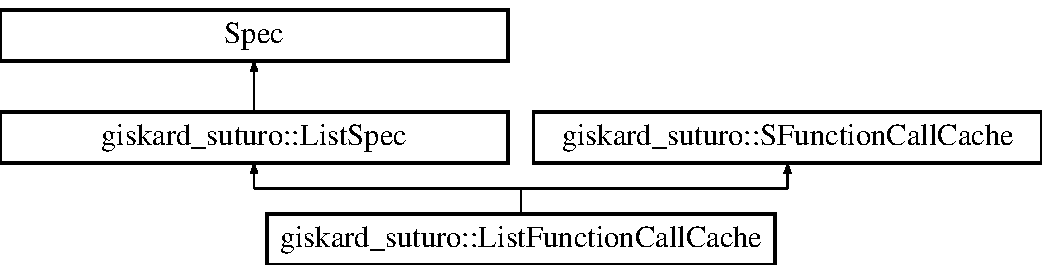
\includegraphics[height=3.000000cm]{classgiskard__suturo_1_1ListFunctionCallCache}
\end{center}
\end{figure}
\subsection*{Public Member Functions}
\begin{DoxyCompactItemize}
\item 
\hypertarget{classgiskard__suturo_1_1ListFunctionCallCache_a19bba5c6ba7ab1a8273662594ccdc47a}{{\bfseries List\-Function\-Call\-Cache} (std\-::vector$<$ Spec\-Ptr $>$ \-\_\-arguments, Fn\-Def\-Ptr \-\_\-fn\-Def)}\label{classgiskard__suturo_1_1ListFunctionCallCache_a19bba5c6ba7ab1a8273662594ccdc47a}

\item 
\hypertarget{classgiskard__suturo_1_1ListFunctionCallCache_ae0cf5c8642bb9c43c7fab54e7c03c91b}{virtual bool {\bfseries equals} (const Spec \&other) const }\label{classgiskard__suturo_1_1ListFunctionCallCache_ae0cf5c8642bb9c43c7fab54e7c03c91b}

\item 
\hypertarget{classgiskard__suturo_1_1ListFunctionCallCache_a0dd12fdd635f043a5d7c538272ca88db}{void {\bfseries get\-\_\-input\-\_\-specs} (std\-::vector$<$ const Input\-Spec $\ast$ $>$ \&inputs) const }\label{classgiskard__suturo_1_1ListFunctionCallCache_a0dd12fdd635f043a5d7c538272ca88db}

\item 
\hypertarget{classgiskard__suturo_1_1ListFunctionCallCache_a34c5a6ce86a28d706eb3cc35a39eeb37}{std\-::vector$<$ Spec\-Ptr $>$ {\bfseries get\-\_\-value} () const }\label{classgiskard__suturo_1_1ListFunctionCallCache_a34c5a6ce86a28d706eb3cc35a39eeb37}

\item 
const Spec\-Ptr \hyperlink{classgiskard__suturo_1_1ListFunctionCallCache_a2c1027c8c47611420120e447a9e183f1}{inner\-Type} () const 
\begin{DoxyCompactList}\small\item\em Returns pointer determining the type of the list's contents. \end{DoxyCompactList}\end{DoxyCompactItemize}
\subsection*{Additional Inherited Members}


\subsection{Detailed Description}
Function call cache for list functions. 

\subsection{Member Function Documentation}
\hypertarget{classgiskard__suturo_1_1ListFunctionCallCache_a2c1027c8c47611420120e447a9e183f1}{\index{giskard\-\_\-suturo\-::\-List\-Function\-Call\-Cache@{giskard\-\_\-suturo\-::\-List\-Function\-Call\-Cache}!inner\-Type@{inner\-Type}}
\index{inner\-Type@{inner\-Type}!giskard_suturo::ListFunctionCallCache@{giskard\-\_\-suturo\-::\-List\-Function\-Call\-Cache}}
\subsubsection[{inner\-Type}]{\setlength{\rightskip}{0pt plus 5cm}const Spec\-Ptr giskard\-\_\-suturo\-::\-List\-Function\-Call\-Cache\-::inner\-Type (
\begin{DoxyParamCaption}
{}
\end{DoxyParamCaption}
) const\hspace{0.3cm}{\ttfamily [inline]}, {\ttfamily [virtual]}}}\label{classgiskard__suturo_1_1ListFunctionCallCache_a2c1027c8c47611420120e447a9e183f1}


Returns pointer determining the type of the list's contents. 

\begin{DoxyReturn}{Returns}
Type pointer 
\end{DoxyReturn}


Implements \hyperlink{classgiskard__suturo_1_1ListSpec_aba0a625da0d48e702aa723fb6fb3bc7e}{giskard\-\_\-suturo\-::\-List\-Spec}.



The documentation for this class was generated from the following file\-:\begin{DoxyCompactItemize}
\item 
giskard\-\_\-suturo\-\_\-parser/include/giskard\-\_\-suturo\-\_\-parser/functions.\-h\end{DoxyCompactItemize}

\hypertarget{classgiskard__suturo_1_1ListReferenceSpec}{\section{giskard\-\_\-suturo\-:\-:List\-Reference\-Spec Class Reference}
\label{classgiskard__suturo_1_1ListReferenceSpec}\index{giskard\-\_\-suturo\-::\-List\-Reference\-Spec@{giskard\-\_\-suturo\-::\-List\-Reference\-Spec}}
}


Reference for list specifications.  




{\ttfamily \#include $<$specifications.\-h$>$}

Inheritance diagram for giskard\-\_\-suturo\-:\-:List\-Reference\-Spec\-:\begin{figure}[H]
\begin{center}
\leavevmode
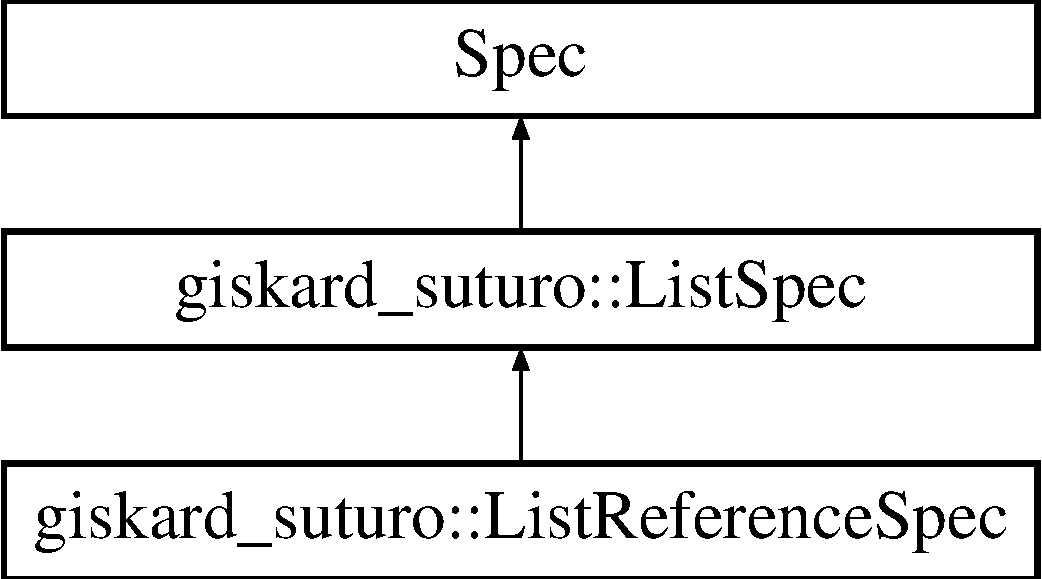
\includegraphics[height=3.000000cm]{classgiskard__suturo_1_1ListReferenceSpec}
\end{center}
\end{figure}
\subsection*{Public Member Functions}
\begin{DoxyCompactItemize}
\item 
\hypertarget{classgiskard__suturo_1_1ListReferenceSpec_aae66215922b554ca789d9c773483413c}{{\bfseries List\-Reference\-Spec} (const std\-::string \&ref\-Name, const boost\-::shared\-\_\-ptr$<$ \hyperlink{classgiskard__suturo_1_1AdvancedScope}{Advanced\-Scope} $>$ \&\-\_\-scope, const Spec\-Ptr \&\-\_\-inner\-Type)}\label{classgiskard__suturo_1_1ListReferenceSpec_aae66215922b554ca789d9c773483413c}

\item 
const Spec\-Ptr \hyperlink{classgiskard__suturo_1_1ListReferenceSpec_a6f7600a285633f7ef19c0a13f0236ae6}{inner\-Type} () const 
\begin{DoxyCompactList}\small\item\em Returns pointer determining the type of the list's contents. \end{DoxyCompactList}\item 
\hypertarget{classgiskard__suturo_1_1ListReferenceSpec_a172fc228b1113d0d1ed33acc5ac35863}{const std\-::string \& {\bfseries get\-\_\-reference\-\_\-name} () const }\label{classgiskard__suturo_1_1ListReferenceSpec_a172fc228b1113d0d1ed33acc5ac35863}

\item 
\hypertarget{classgiskard__suturo_1_1ListReferenceSpec_a386521c134951201eefd91714aab63bf}{void {\bfseries set\-\_\-reference\-\_\-name} (const std\-::string \&ref\-Name)}\label{classgiskard__suturo_1_1ListReferenceSpec_a386521c134951201eefd91714aab63bf}

\item 
\hypertarget{classgiskard__suturo_1_1ListReferenceSpec_addbdde137c2005fb0555b900d856bc02}{void {\bfseries get\-\_\-input\-\_\-specs} (std\-::vector$<$ const Input\-Spec $\ast$ $>$ \&inputs) const }\label{classgiskard__suturo_1_1ListReferenceSpec_addbdde137c2005fb0555b900d856bc02}

\item 
\hypertarget{classgiskard__suturo_1_1ListReferenceSpec_a1b13096cfe83dc628d833b9e0cc752ba}{bool {\bfseries equals} (const Spec \&other) const }\label{classgiskard__suturo_1_1ListReferenceSpec_a1b13096cfe83dc628d833b9e0cc752ba}

\item 
\hypertarget{classgiskard__suturo_1_1ListReferenceSpec_a2a46f259dc474644b4c732d59d3c360a}{std\-::vector$<$ Spec\-Ptr $>$ {\bfseries get\-\_\-value} () const }\label{classgiskard__suturo_1_1ListReferenceSpec_a2a46f259dc474644b4c732d59d3c360a}

\item 
\hypertarget{classgiskard__suturo_1_1ListReferenceSpec_ac5bdd2941128d57c97bbbaa2956db3d0}{const boost\-::shared\-\_\-ptr\\*
$<$ \hyperlink{classgiskard__suturo_1_1AdvancedScope}{Advanced\-Scope} $>$ \& {\bfseries get\-Scope} () const }\label{classgiskard__suturo_1_1ListReferenceSpec_ac5bdd2941128d57c97bbbaa2956db3d0}

\end{DoxyCompactItemize}
\subsection*{Private Attributes}
\begin{DoxyCompactItemize}
\item 
\hypertarget{classgiskard__suturo_1_1ListReferenceSpec_a83b3cd8ce3b86e6258b87061f781f51b}{Spec\-Ptr {\bfseries inner\-T}}\label{classgiskard__suturo_1_1ListReferenceSpec_a83b3cd8ce3b86e6258b87061f781f51b}

\item 
\hypertarget{classgiskard__suturo_1_1ListReferenceSpec_abfd3c34800480d1eaa53a4cb1d006b58}{boost\-::shared\-\_\-ptr$<$ \hyperlink{classgiskard__suturo_1_1AdvancedScope}{Advanced\-Scope} $>$ {\bfseries scope}}\label{classgiskard__suturo_1_1ListReferenceSpec_abfd3c34800480d1eaa53a4cb1d006b58}

\item 
\hypertarget{classgiskard__suturo_1_1ListReferenceSpec_a8733f7b3d94d623a2f18164ff8045b7e}{std\-::string {\bfseries reference\-\_\-name}}\label{classgiskard__suturo_1_1ListReferenceSpec_a8733f7b3d94d623a2f18164ff8045b7e}

\end{DoxyCompactItemize}


\subsection{Detailed Description}
Reference for list specifications. 

\subsection{Member Function Documentation}
\hypertarget{classgiskard__suturo_1_1ListReferenceSpec_a6f7600a285633f7ef19c0a13f0236ae6}{\index{giskard\-\_\-suturo\-::\-List\-Reference\-Spec@{giskard\-\_\-suturo\-::\-List\-Reference\-Spec}!inner\-Type@{inner\-Type}}
\index{inner\-Type@{inner\-Type}!giskard_suturo::ListReferenceSpec@{giskard\-\_\-suturo\-::\-List\-Reference\-Spec}}
\subsubsection[{inner\-Type}]{\setlength{\rightskip}{0pt plus 5cm}const Spec\-Ptr giskard\-\_\-suturo\-::\-List\-Reference\-Spec\-::inner\-Type (
\begin{DoxyParamCaption}
{}
\end{DoxyParamCaption}
) const\hspace{0.3cm}{\ttfamily [inline]}, {\ttfamily [virtual]}}}\label{classgiskard__suturo_1_1ListReferenceSpec_a6f7600a285633f7ef19c0a13f0236ae6}


Returns pointer determining the type of the list's contents. 

\begin{DoxyReturn}{Returns}
Type pointer 
\end{DoxyReturn}


Implements \hyperlink{classgiskard__suturo_1_1ListSpec_aba0a625da0d48e702aa723fb6fb3bc7e}{giskard\-\_\-suturo\-::\-List\-Spec}.



The documentation for this class was generated from the following files\-:\begin{DoxyCompactItemize}
\item 
giskard\-\_\-suturo\-\_\-parser/include/giskard\-\_\-suturo\-\_\-parser/specifications.\-h\item 
giskard\-\_\-suturo\-\_\-parser/src/specifications.\-cpp\end{DoxyCompactItemize}

\hypertarget{classgiskard__suturo_1_1ListSpec}{\section{giskard\-\_\-suturo\-:\-:List\-Spec Class Reference}
\label{classgiskard__suturo_1_1ListSpec}\index{giskard\-\_\-suturo\-::\-List\-Spec@{giskard\-\_\-suturo\-::\-List\-Spec}}
}


Super class for list specifications.  




{\ttfamily \#include $<$specifications.\-h$>$}

Inheritance diagram for giskard\-\_\-suturo\-:\-:List\-Spec\-:\begin{figure}[H]
\begin{center}
\leavevmode
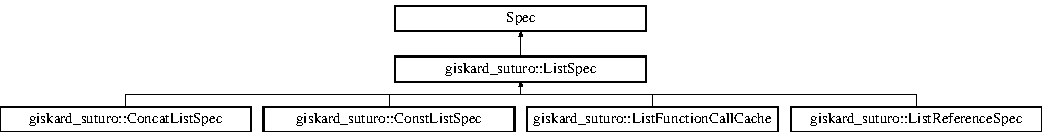
\includegraphics[height=1.779661cm]{classgiskard__suturo_1_1ListSpec}
\end{center}
\end{figure}
\subsection*{Public Member Functions}
\begin{DoxyCompactItemize}
\item 
\hypertarget{classgiskard__suturo_1_1ListSpec_abffa4ce634ef502a00284916b2464c28}{virtual std\-::vector$<$ Spec\-Ptr $>$ {\bfseries get\-\_\-value} () const =0}\label{classgiskard__suturo_1_1ListSpec_abffa4ce634ef502a00284916b2464c28}

\item 
virtual const Spec\-Ptr \hyperlink{classgiskard__suturo_1_1ListSpec_aba0a625da0d48e702aa723fb6fb3bc7e}{inner\-Type} () const =0
\begin{DoxyCompactList}\small\item\em Returns pointer determining the type of the list's contents. \end{DoxyCompactList}\end{DoxyCompactItemize}


\subsection{Detailed Description}
Super class for list specifications. 

\subsection{Member Function Documentation}
\hypertarget{classgiskard__suturo_1_1ListSpec_aba0a625da0d48e702aa723fb6fb3bc7e}{\index{giskard\-\_\-suturo\-::\-List\-Spec@{giskard\-\_\-suturo\-::\-List\-Spec}!inner\-Type@{inner\-Type}}
\index{inner\-Type@{inner\-Type}!giskard_suturo::ListSpec@{giskard\-\_\-suturo\-::\-List\-Spec}}
\subsubsection[{inner\-Type}]{\setlength{\rightskip}{0pt plus 5cm}virtual const Spec\-Ptr giskard\-\_\-suturo\-::\-List\-Spec\-::inner\-Type (
\begin{DoxyParamCaption}
{}
\end{DoxyParamCaption}
) const\hspace{0.3cm}{\ttfamily [pure virtual]}}}\label{classgiskard__suturo_1_1ListSpec_aba0a625da0d48e702aa723fb6fb3bc7e}


Returns pointer determining the type of the list's contents. 

\begin{DoxyReturn}{Returns}
Type pointer 
\end{DoxyReturn}


Implemented in \hyperlink{classgiskard__suturo_1_1ListFunctionCallCache_a2c1027c8c47611420120e447a9e183f1}{giskard\-\_\-suturo\-::\-List\-Function\-Call\-Cache}, \hyperlink{classgiskard__suturo_1_1ConcatListSpec_ab4c15638659af22f9bfc4676e4e7b399}{giskard\-\_\-suturo\-::\-Concat\-List\-Spec}, \hyperlink{classgiskard__suturo_1_1ConstListSpec_a1373658498d2aa8fe4278daa4950968e}{giskard\-\_\-suturo\-::\-Const\-List\-Spec}, and \hyperlink{classgiskard__suturo_1_1ListReferenceSpec_a6f7600a285633f7ef19c0a13f0236ae6}{giskard\-\_\-suturo\-::\-List\-Reference\-Spec}.



The documentation for this class was generated from the following file\-:\begin{DoxyCompactItemize}
\item 
giskard\-\_\-suturo\-\_\-parser/include/giskard\-\_\-suturo\-\_\-parser/specifications.\-h\end{DoxyCompactItemize}

\hypertarget{classMutexMap}{\section{Mutex\-Map$<$ K, V $>$ Class Template Reference}
\label{classMutexMap}\index{Mutex\-Map$<$ K, V $>$@{Mutex\-Map$<$ K, V $>$}}
}
\subsection*{Public Member Functions}
\begin{DoxyCompactItemize}
\item 
\hypertarget{classMutexMap_a8a3c932f1158bf476446dd65e789ee0d}{void {\bfseries set} (const K \&key, V \&value)}\label{classMutexMap_a8a3c932f1158bf476446dd65e789ee0d}

\item 
\hypertarget{classMutexMap_a5113371874f6df8db201c5b40365e2ac}{bool {\bfseries get} (const K \&key, V \&value)}\label{classMutexMap_a5113371874f6df8db201c5b40365e2ac}

\item 
\hypertarget{classMutexMap_aa47c8dfe143b551c93bd8ea61ce27627}{void {\bfseries clear} ()}\label{classMutexMap_aa47c8dfe143b551c93bd8ea61ce27627}

\end{DoxyCompactItemize}
\subsection*{Private Attributes}
\begin{DoxyCompactItemize}
\item 
\hypertarget{classMutexMap_a75dda3d7c21b3cb689c331b5bbaad117}{mutex {\bfseries mtex}}\label{classMutexMap_a75dda3d7c21b3cb689c331b5bbaad117}

\item 
\hypertarget{classMutexMap_a3c9466093fa30dc59e55e4eb1c34c42f}{unordered\-\_\-map$<$ K, V $>$ {\bfseries map}}\label{classMutexMap_a3c9466093fa30dc59e55e4eb1c34c42f}

\end{DoxyCompactItemize}


The documentation for this class was generated from the following file\-:\begin{DoxyCompactItemize}
\item 
suturo\-\_\-action\-\_\-server/include/suturo\-\_\-action\-\_\-server/Collision\-Scene.\-h\end{DoxyCompactItemize}

\hypertarget{classsuturo__octree_1_1Node}{\section{suturo\-\_\-octree\-:\-:Node Class Reference}
\label{classsuturo__octree_1_1Node}\index{suturo\-\_\-octree\-::\-Node@{suturo\-\_\-octree\-::\-Node}}
}
\subsection*{Public Member Functions}
\begin{DoxyCompactItemize}
\item 
\hyperlink{classsuturo__octree_1_1Node_ad950cd5ccb6fe1c8276407594543e780}{Node} (\hyperlink{structPoint3f}{Point3f} center, bool is\-Occupied, int \hyperlink{classsuturo__octree_1_1Node_af165133c7b374ce9d7204f7fb1c61921}{is\-Leaf})
\begin{DoxyCompactList}\small\item\em Constructs the \hyperlink{classsuturo__octree_1_1Node}{Node}. \end{DoxyCompactList}\item 
\hypertarget{classsuturo__octree_1_1Node_aa4a574ba768c3e6132f500230d3b4e23}{\hyperlink{classsuturo__octree_1_1Node_aa4a574ba768c3e6132f500230d3b4e23}{Node} ()}\label{classsuturo__octree_1_1Node_aa4a574ba768c3e6132f500230d3b4e23}

\begin{DoxyCompactList}\small\item\em Constructs the object. \end{DoxyCompactList}\item 
\hypertarget{classsuturo__octree_1_1Node_a8a189b19875b114835a817a005a06f46}{bool {\bfseries is\-Occupied} ()}\label{classsuturo__octree_1_1Node_a8a189b19875b114835a817a005a06f46}

\item 
void \hyperlink{classsuturo__octree_1_1Node_a79a8372a6a141a9b26817a059da3ee53}{is\-Occupied} (bool oc)
\begin{DoxyCompactList}\small\item\em Sets the occupancy of the \hyperlink{classsuturo__octree_1_1Node}{Node}. \end{DoxyCompactList}\item 
bool \hyperlink{classsuturo__octree_1_1Node_af165133c7b374ce9d7204f7fb1c61921}{is\-Leaf} ()
\begin{DoxyCompactList}\small\item\em Determines if leaf. \end{DoxyCompactList}\item 
\hyperlink{classsuturo__octree_1_1Node}{Node} $\ast$\& \hyperlink{classsuturo__octree_1_1Node_a4ba1c3546ad6966b420b9d5b8c11381d}{operator\mbox{[}$\,$\mbox{]}} (int idx)
\begin{DoxyCompactList}\small\item\em Returns a pointer the the idxs child of the \hyperlink{classsuturo__octree_1_1Node}{Node}. \end{DoxyCompactList}\item 
\hyperlink{structPoint3f}{Point3f} \hyperlink{classsuturo__octree_1_1Node_ace47b8d3f9048d75390f50b6ccde3a74}{get\-Center} ()
\begin{DoxyCompactList}\small\item\em Returns the center of the \hyperlink{classsuturo__octree_1_1Node}{Node}. \end{DoxyCompactList}\end{DoxyCompactItemize}
\subsection*{Private Attributes}
\begin{DoxyCompactItemize}
\item 
\hypertarget{classsuturo__octree_1_1Node_a51d9a6fe2a7f8c5e46777a692c6f0d9c}{\hyperlink{classsuturo__octree_1_1Node}{Node} $\ast$ {\bfseries child0}}\label{classsuturo__octree_1_1Node_a51d9a6fe2a7f8c5e46777a692c6f0d9c}

\item 
\hypertarget{classsuturo__octree_1_1Node_a95679183fda704cb527ca4e728d2a64b}{\hyperlink{classsuturo__octree_1_1Node}{Node} $\ast$ {\bfseries child1}}\label{classsuturo__octree_1_1Node_a95679183fda704cb527ca4e728d2a64b}

\item 
\hypertarget{classsuturo__octree_1_1Node_a57686204a7b3cad6652436f7addab913}{\hyperlink{classsuturo__octree_1_1Node}{Node} $\ast$ {\bfseries child2}}\label{classsuturo__octree_1_1Node_a57686204a7b3cad6652436f7addab913}

\item 
\hypertarget{classsuturo__octree_1_1Node_aa5ee749044e8640027c8827f44881589}{\hyperlink{classsuturo__octree_1_1Node}{Node} $\ast$ {\bfseries child3}}\label{classsuturo__octree_1_1Node_aa5ee749044e8640027c8827f44881589}

\item 
\hypertarget{classsuturo__octree_1_1Node_a572c7894f54eaecbdda220c395741ab1}{\hyperlink{classsuturo__octree_1_1Node}{Node} $\ast$ {\bfseries child4}}\label{classsuturo__octree_1_1Node_a572c7894f54eaecbdda220c395741ab1}

\item 
\hypertarget{classsuturo__octree_1_1Node_a0c4e0a7488eaf1e69a669d04cf9e903b}{\hyperlink{classsuturo__octree_1_1Node}{Node} $\ast$ {\bfseries child5}}\label{classsuturo__octree_1_1Node_a0c4e0a7488eaf1e69a669d04cf9e903b}

\item 
\hypertarget{classsuturo__octree_1_1Node_a6a1c6166b17d1ff6cb51aa866d359459}{\hyperlink{classsuturo__octree_1_1Node}{Node} $\ast$ {\bfseries child6}}\label{classsuturo__octree_1_1Node_a6a1c6166b17d1ff6cb51aa866d359459}

\item 
\hypertarget{classsuturo__octree_1_1Node_a86d0e710b222e3909f624928adc37160}{\hyperlink{classsuturo__octree_1_1Node}{Node} $\ast$ {\bfseries child7}}\label{classsuturo__octree_1_1Node_a86d0e710b222e3909f624928adc37160}

\item 
\hypertarget{classsuturo__octree_1_1Node_a11e1325064625141f0a99471c3a88227}{bool {\bfseries leaf}}\label{classsuturo__octree_1_1Node_a11e1325064625141f0a99471c3a88227}

\item 
\hypertarget{classsuturo__octree_1_1Node_adba7d01ac5f68818d3f52a66fb6f1827}{bool {\bfseries occupied}}\label{classsuturo__octree_1_1Node_adba7d01ac5f68818d3f52a66fb6f1827}

\item 
\hypertarget{classsuturo__octree_1_1Node_a471d6216990e378c8920d5df47922891}{\hyperlink{structPoint3f}{Point3f} {\bfseries center}}\label{classsuturo__octree_1_1Node_a471d6216990e378c8920d5df47922891}

\end{DoxyCompactItemize}


\subsection{Constructor \& Destructor Documentation}
\hypertarget{classsuturo__octree_1_1Node_ad950cd5ccb6fe1c8276407594543e780}{\index{suturo\-\_\-octree\-::\-Node@{suturo\-\_\-octree\-::\-Node}!Node@{Node}}
\index{Node@{Node}!suturo_octree::Node@{suturo\-\_\-octree\-::\-Node}}
\subsubsection[{Node}]{\setlength{\rightskip}{0pt plus 5cm}suturo\-\_\-octree\-::\-Node\-::\-Node (
\begin{DoxyParamCaption}
\item[{{\bf Point3f}}]{center, }
\item[{bool}]{is\-Occupied, }
\item[{int}]{is\-Leaf}
\end{DoxyParamCaption}
)}}\label{classsuturo__octree_1_1Node_ad950cd5ccb6fe1c8276407594543e780}


Constructs the \hyperlink{classsuturo__octree_1_1Node}{Node}. 


\begin{DoxyParams}[1]{Parameters}
\mbox{\tt in}  & {\em center} & The center of the \hyperlink{classsuturo__octree_1_1Node}{Node} \\
\hline
\mbox{\tt in}  & {\em is\-Occupied} & Indicates if occupied \\
\hline
\mbox{\tt in}  & {\em is\-Leaf} & Indicates if this \hyperlink{classsuturo__octree_1_1Node}{Node} is a leaf \hyperlink{classsuturo__octree_1_1Node}{Node} \\
\hline
\end{DoxyParams}


\subsection{Member Function Documentation}
\hypertarget{classsuturo__octree_1_1Node_ace47b8d3f9048d75390f50b6ccde3a74}{\index{suturo\-\_\-octree\-::\-Node@{suturo\-\_\-octree\-::\-Node}!get\-Center@{get\-Center}}
\index{get\-Center@{get\-Center}!suturo_octree::Node@{suturo\-\_\-octree\-::\-Node}}
\subsubsection[{get\-Center}]{\setlength{\rightskip}{0pt plus 5cm}{\bf Point3f} suturo\-\_\-octree\-::\-Node\-::get\-Center (
\begin{DoxyParamCaption}
{}
\end{DoxyParamCaption}
)}}\label{classsuturo__octree_1_1Node_ace47b8d3f9048d75390f50b6ccde3a74}


Returns the center of the \hyperlink{classsuturo__octree_1_1Node}{Node}. 

\begin{DoxyReturn}{Returns}
The center. 
\end{DoxyReturn}
\hypertarget{classsuturo__octree_1_1Node_af165133c7b374ce9d7204f7fb1c61921}{\index{suturo\-\_\-octree\-::\-Node@{suturo\-\_\-octree\-::\-Node}!is\-Leaf@{is\-Leaf}}
\index{is\-Leaf@{is\-Leaf}!suturo_octree::Node@{suturo\-\_\-octree\-::\-Node}}
\subsubsection[{is\-Leaf}]{\setlength{\rightskip}{0pt plus 5cm}bool suturo\-\_\-octree\-::\-Node\-::is\-Leaf (
\begin{DoxyParamCaption}
{}
\end{DoxyParamCaption}
)}}\label{classsuturo__octree_1_1Node_af165133c7b374ce9d7204f7fb1c61921}


Determines if leaf. 

\begin{DoxyReturn}{Returns}
True if leaf, False otherwise. 
\end{DoxyReturn}
\hypertarget{classsuturo__octree_1_1Node_a79a8372a6a141a9b26817a059da3ee53}{\index{suturo\-\_\-octree\-::\-Node@{suturo\-\_\-octree\-::\-Node}!is\-Occupied@{is\-Occupied}}
\index{is\-Occupied@{is\-Occupied}!suturo_octree::Node@{suturo\-\_\-octree\-::\-Node}}
\subsubsection[{is\-Occupied}]{\setlength{\rightskip}{0pt plus 5cm}void suturo\-\_\-octree\-::\-Node\-::is\-Occupied (
\begin{DoxyParamCaption}
\item[{bool}]{oc}
\end{DoxyParamCaption}
)}}\label{classsuturo__octree_1_1Node_a79a8372a6a141a9b26817a059da3ee53}


Sets the occupancy of the \hyperlink{classsuturo__octree_1_1Node}{Node}. 


\begin{DoxyParams}[1]{Parameters}
\mbox{\tt in}  & {\em oc} & \{ parameter\-\_\-description \} \\
\hline
\end{DoxyParams}
\hypertarget{classsuturo__octree_1_1Node_a4ba1c3546ad6966b420b9d5b8c11381d}{\index{suturo\-\_\-octree\-::\-Node@{suturo\-\_\-octree\-::\-Node}!operator\mbox{[}$\,$\mbox{]}@{operator[]}}
\index{operator\mbox{[}$\,$\mbox{]}@{operator[]}!suturo_octree::Node@{suturo\-\_\-octree\-::\-Node}}
\subsubsection[{operator[]}]{\setlength{\rightskip}{0pt plus 5cm}{\bf Node} $\ast$\& suturo\-\_\-octree\-::\-Node\-::operator\mbox{[}$\,$\mbox{]} (
\begin{DoxyParamCaption}
\item[{int}]{idx}
\end{DoxyParamCaption}
)}}\label{classsuturo__octree_1_1Node_a4ba1c3546ad6966b420b9d5b8c11381d}


Returns a pointer the the idxs child of the \hyperlink{classsuturo__octree_1_1Node}{Node}. 


\begin{DoxyParams}[1]{Parameters}
\mbox{\tt in}  & {\em idx} & The index\\
\hline
\end{DoxyParams}
\begin{DoxyReturn}{Returns}
A pointer the the idxs child of the \hyperlink{classsuturo__octree_1_1Node}{Node}. 
\end{DoxyReturn}


The documentation for this class was generated from the following files\-:\begin{DoxyCompactItemize}
\item 
suturo\-\_\-action\-\_\-server/include/suturo\-\_\-action\-\_\-server/Node.\-h\item 
suturo\-\_\-action\-\_\-server/src/Node.\-cpp\end{DoxyCompactItemize}

\hypertarget{structgiskard__suturo_1_1NotImplementedException}{\section{giskard\-\_\-suturo\-:\-:Not\-Implemented\-Exception Struct Reference}
\label{structgiskard__suturo_1_1NotImplementedException}\index{giskard\-\_\-suturo\-::\-Not\-Implemented\-Exception@{giskard\-\_\-suturo\-::\-Not\-Implemented\-Exception}}
}
Inheritance diagram for giskard\-\_\-suturo\-:\-:Not\-Implemented\-Exception\-:\begin{figure}[H]
\begin{center}
\leavevmode
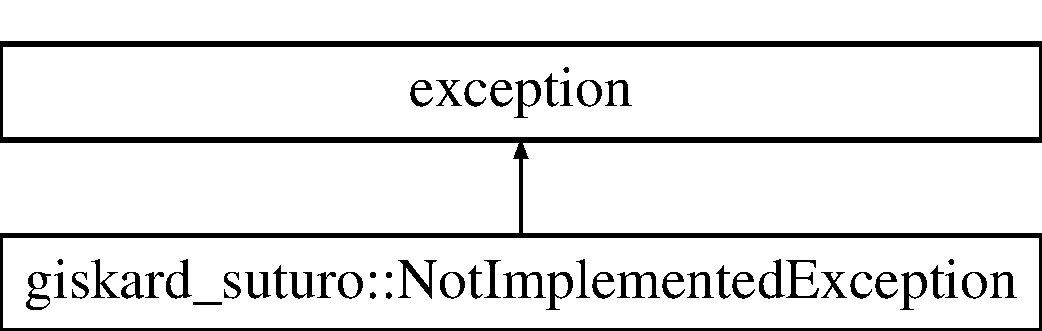
\includegraphics[height=2.000000cm]{structgiskard__suturo_1_1NotImplementedException}
\end{center}
\end{figure}
\subsection*{Public Member Functions}
\begin{DoxyCompactItemize}
\item 
\hypertarget{structgiskard__suturo_1_1NotImplementedException_a821b94fe0ed0034c9d63e9f985b1aa97}{const char $\ast$ {\bfseries what} () noexcept}\label{structgiskard__suturo_1_1NotImplementedException_a821b94fe0ed0034c9d63e9f985b1aa97}

\end{DoxyCompactItemize}


The documentation for this struct was generated from the following file\-:\begin{DoxyCompactItemize}
\item 
giskard\-\_\-suturo\-\_\-parser/include/giskard\-\_\-suturo\-\_\-parser/utils.\-h\end{DoxyCompactItemize}

\hypertarget{classsuturo__octree_1_1Octree}{\section{suturo\-\_\-octree\-:\-:Octree Class Reference}
\label{classsuturo__octree_1_1Octree}\index{suturo\-\_\-octree\-::\-Octree@{suturo\-\_\-octree\-::\-Octree}}
}
\subsection*{Public Member Functions}
\begin{DoxyCompactItemize}
\item 
\hyperlink{classsuturo__octree_1_1Octree_a7d363eb4bbc6179098a03ea09a569711}{Octree} (float size, int depth, \hyperlink{structPoint3f}{Point3f} center)
\begin{DoxyCompactList}\small\item\em Constructs the octree. \end{DoxyCompactList}\item 
void \hyperlink{classsuturo__octree_1_1Octree_aa142de332240f77c5ed0b3911645f715}{add\-Point} (\hyperlink{structPoint3f}{Point3f} point)
\begin{DoxyCompactList}\small\item\em Marks the leaf node and every parent at the coordinate of the point as occupied. \end{DoxyCompactList}\item 
\hyperlink{classsuturo__octree_1_1Node}{suturo\-\_\-octree\-::\-Node} $\ast$ \hyperlink{classsuturo__octree_1_1Octree_a9a685337a49698151441ccca37067ca5}{get\-Root} ()
\begin{DoxyCompactList}\small\item\em Returns the root node of the octree. \end{DoxyCompactList}\item 
int \hyperlink{classsuturo__octree_1_1Octree_a2061177532684f240b75214e4b20e947}{get\-Depth} ()
\begin{DoxyCompactList}\small\item\em Returns the depth of the octree. \end{DoxyCompactList}\item 
float \hyperlink{classsuturo__octree_1_1Octree_aa3c6fced22f53e2ee09aad80595d9ff7}{get\-Size} ()
\begin{DoxyCompactList}\small\item\em Returns the size of the octree. \end{DoxyCompactList}\end{DoxyCompactItemize}
\subsection*{Private Member Functions}
\begin{DoxyCompactItemize}
\item 
\hypertarget{classsuturo__octree_1_1Octree_ac961e889dc458f61ff16e20fd2a23556}{void {\bfseries init} ()}\label{classsuturo__octree_1_1Octree_ac961e889dc458f61ff16e20fd2a23556}

\end{DoxyCompactItemize}
\subsection*{Private Attributes}
\begin{DoxyCompactItemize}
\item 
\hypertarget{classsuturo__octree_1_1Octree_a7fa7fd311008f45b8dc1dea3fbc4c30e}{\hyperlink{classsuturo__octree_1_1Node}{suturo\-\_\-octree\-::\-Node} $\ast$ {\bfseries root\-Node}}\label{classsuturo__octree_1_1Octree_a7fa7fd311008f45b8dc1dea3fbc4c30e}

\item 
\hypertarget{classsuturo__octree_1_1Octree_aea09855bd32b713bd21b5c94d230757e}{float {\bfseries size}}\label{classsuturo__octree_1_1Octree_aea09855bd32b713bd21b5c94d230757e}

\item 
\hypertarget{classsuturo__octree_1_1Octree_a143d54ed6aac1154550d377796db13b3}{\hyperlink{structPoint3f}{Point3f} {\bfseries center}}\label{classsuturo__octree_1_1Octree_a143d54ed6aac1154550d377796db13b3}

\item 
\hypertarget{classsuturo__octree_1_1Octree_abd0bdf0192e6a7d1388040b13b7ec332}{int {\bfseries depth}}\label{classsuturo__octree_1_1Octree_abd0bdf0192e6a7d1388040b13b7ec332}

\end{DoxyCompactItemize}


\subsection{Constructor \& Destructor Documentation}
\hypertarget{classsuturo__octree_1_1Octree_a7d363eb4bbc6179098a03ea09a569711}{\index{suturo\-\_\-octree\-::\-Octree@{suturo\-\_\-octree\-::\-Octree}!Octree@{Octree}}
\index{Octree@{Octree}!suturo_octree::Octree@{suturo\-\_\-octree\-::\-Octree}}
\subsubsection[{Octree}]{\setlength{\rightskip}{0pt plus 5cm}suturo\-\_\-octree\-::\-Octree\-::\-Octree (
\begin{DoxyParamCaption}
\item[{float}]{size, }
\item[{int}]{depth, }
\item[{{\bf Point3f}}]{center}
\end{DoxyParamCaption}
)}}\label{classsuturo__octree_1_1Octree_a7d363eb4bbc6179098a03ea09a569711}


Constructs the octree. 


\begin{DoxyParams}[1]{Parameters}
\mbox{\tt in}  & {\em size} & The size in m \\
\hline
\mbox{\tt in}  & {\em depth} & The depth \\
\hline
\mbox{\tt in}  & {\em center} & The center of theo ctree \\
\hline
\end{DoxyParams}


\subsection{Member Function Documentation}
\hypertarget{classsuturo__octree_1_1Octree_aa142de332240f77c5ed0b3911645f715}{\index{suturo\-\_\-octree\-::\-Octree@{suturo\-\_\-octree\-::\-Octree}!add\-Point@{add\-Point}}
\index{add\-Point@{add\-Point}!suturo_octree::Octree@{suturo\-\_\-octree\-::\-Octree}}
\subsubsection[{add\-Point}]{\setlength{\rightskip}{0pt plus 5cm}void suturo\-\_\-octree\-::\-Octree\-::add\-Point (
\begin{DoxyParamCaption}
\item[{{\bf Point3f}}]{point}
\end{DoxyParamCaption}
)}}\label{classsuturo__octree_1_1Octree_aa142de332240f77c5ed0b3911645f715}


Marks the leaf node and every parent at the coordinate of the point as occupied. 


\begin{DoxyParams}[1]{Parameters}
\mbox{\tt in}  & {\em point} & The point \\
\hline
\end{DoxyParams}
\hypertarget{classsuturo__octree_1_1Octree_a2061177532684f240b75214e4b20e947}{\index{suturo\-\_\-octree\-::\-Octree@{suturo\-\_\-octree\-::\-Octree}!get\-Depth@{get\-Depth}}
\index{get\-Depth@{get\-Depth}!suturo_octree::Octree@{suturo\-\_\-octree\-::\-Octree}}
\subsubsection[{get\-Depth}]{\setlength{\rightskip}{0pt plus 5cm}int suturo\-\_\-octree\-::\-Octree\-::get\-Depth (
\begin{DoxyParamCaption}
{}
\end{DoxyParamCaption}
)}}\label{classsuturo__octree_1_1Octree_a2061177532684f240b75214e4b20e947}


Returns the depth of the octree. 

\begin{DoxyReturn}{Returns}
The depth 
\end{DoxyReturn}
\hypertarget{classsuturo__octree_1_1Octree_a9a685337a49698151441ccca37067ca5}{\index{suturo\-\_\-octree\-::\-Octree@{suturo\-\_\-octree\-::\-Octree}!get\-Root@{get\-Root}}
\index{get\-Root@{get\-Root}!suturo_octree::Octree@{suturo\-\_\-octree\-::\-Octree}}
\subsubsection[{get\-Root}]{\setlength{\rightskip}{0pt plus 5cm}{\bf Node} $\ast$ suturo\-\_\-octree\-::\-Octree\-::get\-Root (
\begin{DoxyParamCaption}
{}
\end{DoxyParamCaption}
)}}\label{classsuturo__octree_1_1Octree_a9a685337a49698151441ccca37067ca5}


Returns the root node of the octree. 

\begin{DoxyReturn}{Returns}
The root 
\end{DoxyReturn}
\hypertarget{classsuturo__octree_1_1Octree_aa3c6fced22f53e2ee09aad80595d9ff7}{\index{suturo\-\_\-octree\-::\-Octree@{suturo\-\_\-octree\-::\-Octree}!get\-Size@{get\-Size}}
\index{get\-Size@{get\-Size}!suturo_octree::Octree@{suturo\-\_\-octree\-::\-Octree}}
\subsubsection[{get\-Size}]{\setlength{\rightskip}{0pt plus 5cm}float suturo\-\_\-octree\-::\-Octree\-::get\-Size (
\begin{DoxyParamCaption}
{}
\end{DoxyParamCaption}
)}}\label{classsuturo__octree_1_1Octree_aa3c6fced22f53e2ee09aad80595d9ff7}


Returns the size of the octree. 

\begin{DoxyReturn}{Returns}
The size 
\end{DoxyReturn}


The documentation for this class was generated from the following files\-:\begin{DoxyCompactItemize}
\item 
suturo\-\_\-action\-\_\-server/include/suturo\-\_\-action\-\_\-server/Octree.\-h\item 
suturo\-\_\-action\-\_\-server/src/Octree.\-cpp\end{DoxyCompactItemize}

\hypertarget{structgiskard__suturo_1_1GiskardLangParser_1_1ParseException}{\section{giskard\-\_\-suturo\-:\-:Giskard\-Lang\-Parser\-:\-:Parse\-Exception Struct Reference}
\label{structgiskard__suturo_1_1GiskardLangParser_1_1ParseException}\index{giskard\-\_\-suturo\-::\-Giskard\-Lang\-Parser\-::\-Parse\-Exception@{giskard\-\_\-suturo\-::\-Giskard\-Lang\-Parser\-::\-Parse\-Exception}}
}
Inheritance diagram for giskard\-\_\-suturo\-:\-:Giskard\-Lang\-Parser\-:\-:Parse\-Exception\-:\begin{figure}[H]
\begin{center}
\leavevmode
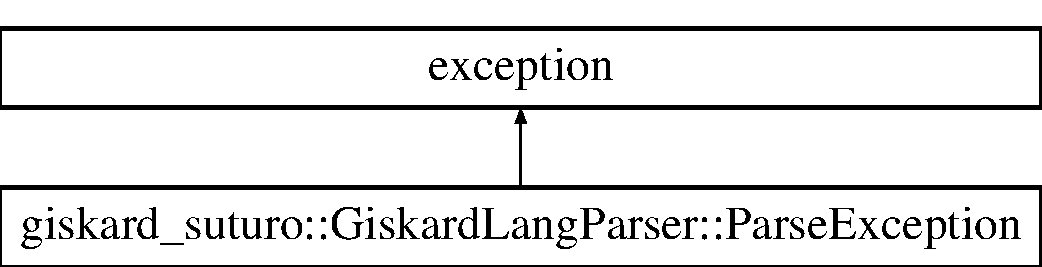
\includegraphics[height=2.000000cm]{structgiskard__suturo_1_1GiskardLangParser_1_1ParseException}
\end{center}
\end{figure}
\subsection*{Public Member Functions}
\begin{DoxyCompactItemize}
\item 
\hypertarget{structgiskard__suturo_1_1GiskardLangParser_1_1ParseException_a35a4313f0b9f6ace6b33ee265ab3c8d8}{{\bfseries Parse\-Exception} (const string \&\-\_\-msg)}\label{structgiskard__suturo_1_1GiskardLangParser_1_1ParseException_a35a4313f0b9f6ace6b33ee265ab3c8d8}

\item 
\hypertarget{structgiskard__suturo_1_1GiskardLangParser_1_1ParseException_a50a25e0644a099970bde101b28c00261}{const char $\ast$ {\bfseries what} () const noexcept}\label{structgiskard__suturo_1_1GiskardLangParser_1_1ParseException_a50a25e0644a099970bde101b28c00261}

\end{DoxyCompactItemize}
\subsection*{Private Attributes}
\begin{DoxyCompactItemize}
\item 
\hypertarget{structgiskard__suturo_1_1GiskardLangParser_1_1ParseException_a2ae4425a5375bf32fd13e95cad65bbd1}{const string {\bfseries msg}}\label{structgiskard__suturo_1_1GiskardLangParser_1_1ParseException_a2ae4425a5375bf32fd13e95cad65bbd1}

\end{DoxyCompactItemize}


The documentation for this struct was generated from the following file\-:\begin{DoxyCompactItemize}
\item 
giskard\-\_\-suturo\-\_\-parser/include/giskard\-\_\-suturo\-\_\-parser/giskard\-\_\-parser.\-hpp\end{DoxyCompactItemize}

\hypertarget{structgiskard__suturo_1_1ParseException}{\section{giskard\-\_\-suturo\-:\-:Parse\-Exception Struct Reference}
\label{structgiskard__suturo_1_1ParseException}\index{giskard\-\_\-suturo\-::\-Parse\-Exception@{giskard\-\_\-suturo\-::\-Parse\-Exception}}
}


Custom wrapper for plain exceptions caused by parsing.  




{\ttfamily \#include $<$parser.\-h$>$}

Inheritance diagram for giskard\-\_\-suturo\-:\-:Parse\-Exception\-:\begin{figure}[H]
\begin{center}
\leavevmode
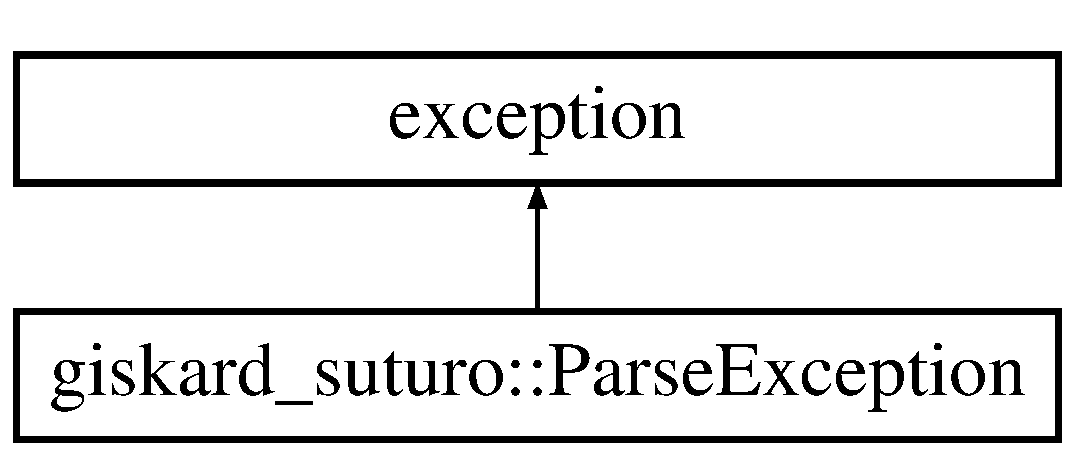
\includegraphics[height=2.000000cm]{structgiskard__suturo_1_1ParseException}
\end{center}
\end{figure}
\subsection*{Public Member Functions}
\begin{DoxyCompactItemize}
\item 
\hypertarget{structgiskard__suturo_1_1ParseException_a1fcd3214c79160e1b3043dd2be1d1f40}{{\bfseries Parse\-Exception} (std\-::string \-\_\-msg)}\label{structgiskard__suturo_1_1ParseException_a1fcd3214c79160e1b3043dd2be1d1f40}

\item 
\hypertarget{structgiskard__suturo_1_1ParseException_a25152a6e0783140f78abc50a28442090}{const char $\ast$ {\bfseries what} () const noexcept}\label{structgiskard__suturo_1_1ParseException_a25152a6e0783140f78abc50a28442090}

\end{DoxyCompactItemize}
\subsection*{Public Attributes}
\begin{DoxyCompactItemize}
\item 
\hypertarget{structgiskard__suturo_1_1ParseException_aaa2d22acb6b0be5d7d037ef591bcbabc}{const std\-::string {\bfseries msg}}\label{structgiskard__suturo_1_1ParseException_aaa2d22acb6b0be5d7d037ef591bcbabc}

\end{DoxyCompactItemize}


\subsection{Detailed Description}
Custom wrapper for plain exceptions caused by parsing. 

The documentation for this struct was generated from the following file\-:\begin{DoxyCompactItemize}
\item 
giskard\-\_\-suturo\-\_\-parser/include/giskard\-\_\-suturo\-\_\-parser/parser.\-h\end{DoxyCompactItemize}

\hypertarget{structPlane}{\section{Plane Struct Reference}
\label{structPlane}\index{Plane@{Plane}}
}
\subsection*{Public Member Functions}
\begin{DoxyCompactItemize}
\item 
\hypertarget{structPlane_ae65b04b0d77541b64d73f4528abc8afd}{C\-U\-D\-A\-\_\-\-C\-A\-L\-L\-A\-B\-L\-E\-\_\-\-M\-E\-M\-B\-E\-R {\bfseries Plane} (float a, float b, float c, float d)}\label{structPlane_ae65b04b0d77541b64d73f4528abc8afd}

\end{DoxyCompactItemize}
\subsection*{Public Attributes}
\begin{DoxyCompactItemize}
\item 
\hypertarget{structPlane_a818b693ba813d53949e18aa1416cc12a}{float {\bfseries a}}\label{structPlane_a818b693ba813d53949e18aa1416cc12a}

\item 
\hypertarget{structPlane_a3d802fea10cfe6352e1792733d793b14}{float {\bfseries b}}\label{structPlane_a3d802fea10cfe6352e1792733d793b14}

\item 
\hypertarget{structPlane_aec04c57607ffa16c210f955360ef4153}{float {\bfseries c}}\label{structPlane_aec04c57607ffa16c210f955360ef4153}

\item 
\hypertarget{structPlane_a61fc789fce8fbe72914f5397f1bbed44}{float {\bfseries d}}\label{structPlane_a61fc789fce8fbe72914f5397f1bbed44}

\end{DoxyCompactItemize}


The documentation for this struct was generated from the following file\-:\begin{DoxyCompactItemize}
\item 
suturo\-\_\-action\-\_\-server/include/suturo\-\_\-action\-\_\-server/Vector3f.\-h\end{DoxyCompactItemize}

\hypertarget{structPoint3f}{\section{Point3f Struct Reference}
\label{structPoint3f}\index{Point3f@{Point3f}}
}
\subsection*{Public Member Functions}
\begin{DoxyCompactItemize}
\item 
\hypertarget{structPoint3f_afd855b46743178dd71288f04512e2c57}{C\-U\-D\-A\-\_\-\-C\-A\-L\-L\-A\-B\-L\-E\-\_\-\-M\-E\-M\-B\-E\-R {\bfseries Point3f} (\hyperlink{structVector3f}{Vector3f} position)}\label{structPoint3f_afd855b46743178dd71288f04512e2c57}

\item 
\hypertarget{structPoint3f_a576c4266e9d7259d801d010fdbbc3306}{C\-U\-D\-A\-\_\-\-C\-A\-L\-L\-A\-B\-L\-E\-\_\-\-M\-E\-M\-B\-E\-R {\bfseries Point3f} (float x, float y, float z)}\label{structPoint3f_a576c4266e9d7259d801d010fdbbc3306}

\end{DoxyCompactItemize}
\subsection*{Public Attributes}
\begin{DoxyCompactItemize}
\item 
\hypertarget{structPoint3f_a7fb9233f46ef9edbcb2c74a83a7828f9}{\hyperlink{structVector3f}{Vector3f} {\bfseries position}}\label{structPoint3f_a7fb9233f46ef9edbcb2c74a83a7828f9}

\end{DoxyCompactItemize}


The documentation for this struct was generated from the following file\-:\begin{DoxyCompactItemize}
\item 
suturo\-\_\-action\-\_\-server/include/suturo\-\_\-action\-\_\-server/Vector3f.\-h\end{DoxyCompactItemize}

\hypertarget{structPoint3fn}{\section{Point3fn Struct Reference}
\label{structPoint3fn}\index{Point3fn@{Point3fn}}
}
\subsection*{Public Member Functions}
\begin{DoxyCompactItemize}
\item 
\hypertarget{structPoint3fn_a2f6d5f3289b86b194656893b853f0ba6}{C\-U\-D\-A\-\_\-\-C\-A\-L\-L\-A\-B\-L\-E\-\_\-\-M\-E\-M\-B\-E\-R {\bfseries Point3fn} (\hyperlink{structVector3f}{Vector3f} position, \hyperlink{structVector3f}{Vector3f} normal)}\label{structPoint3fn_a2f6d5f3289b86b194656893b853f0ba6}

\end{DoxyCompactItemize}
\subsection*{Public Attributes}
\begin{DoxyCompactItemize}
\item 
\hypertarget{structPoint3fn_a87fca59e7907a2b0aaea6f9c403f162a}{\hyperlink{structVector3f}{Vector3f} {\bfseries position}}\label{structPoint3fn_a87fca59e7907a2b0aaea6f9c403f162a}

\item 
\hypertarget{structPoint3fn_af877a85b78f686752acd4b037c8bb6bb}{\hyperlink{structVector3f}{Vector3f} {\bfseries normal}}\label{structPoint3fn_af877a85b78f686752acd4b037c8bb6bb}

\end{DoxyCompactItemize}


The documentation for this struct was generated from the following file\-:\begin{DoxyCompactItemize}
\item 
suturo\-\_\-action\-\_\-server/include/suturo\-\_\-action\-\_\-server/Vector3f.\-h\end{DoxyCompactItemize}

\hypertarget{structGiskardActionServer_1_1posController}{\section{Giskard\-Action\-Server\-:\-:pos\-Controller Struct Reference}
\label{structGiskardActionServer_1_1posController}\index{Giskard\-Action\-Server\-::pos\-Controller@{Giskard\-Action\-Server\-::pos\-Controller}}
}


Internal structure to manage a position controller.  




{\ttfamily \#include $<$Giskard\-Action\-Server.\-h$>$}

\subsection*{Public Attributes}
\begin{DoxyCompactItemize}
\item 
\hypertarget{structGiskardActionServer_1_1posController_a125f1b93bb1a04f498428ce9b906df79}{ros\-::\-Publisher {\bfseries pub}}\label{structGiskardActionServer_1_1posController_a125f1b93bb1a04f498428ce9b906df79}

\item 
\hypertarget{structGiskardActionServer_1_1posController_a78d355a544b03b7e018fc9c1b13273bc}{double {\bfseries d\-T}}\label{structGiskardActionServer_1_1posController_a78d355a544b03b7e018fc9c1b13273bc}

\end{DoxyCompactItemize}


\subsection{Detailed Description}
Internal structure to manage a position controller. 

The documentation for this struct was generated from the following file\-:\begin{DoxyCompactItemize}
\item 
suturo\-\_\-action\-\_\-server/include/suturo\-\_\-action\-\_\-server/Giskard\-Action\-Server.\-h\end{DoxyCompactItemize}

\hypertarget{classgiskard__suturo_1_1RotationFunctionCallCache}{\section{giskard\-\_\-suturo\-:\-:Rotation\-Function\-Call\-Cache Class Reference}
\label{classgiskard__suturo_1_1RotationFunctionCallCache}\index{giskard\-\_\-suturo\-::\-Rotation\-Function\-Call\-Cache@{giskard\-\_\-suturo\-::\-Rotation\-Function\-Call\-Cache}}
}


Function call cache for rotation functions.  




{\ttfamily \#include $<$functions.\-h$>$}

Inheritance diagram for giskard\-\_\-suturo\-:\-:Rotation\-Function\-Call\-Cache\-:\begin{figure}[H]
\begin{center}
\leavevmode
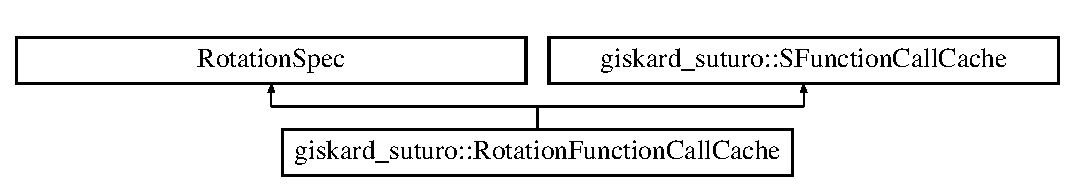
\includegraphics[height=2.000000cm]{classgiskard__suturo_1_1RotationFunctionCallCache}
\end{center}
\end{figure}
\subsection*{Public Member Functions}
\begin{DoxyCompactItemize}
\item 
\hypertarget{classgiskard__suturo_1_1RotationFunctionCallCache_a9c76b124b063a8b07ace19c21750d946}{{\bfseries Rotation\-Function\-Call\-Cache} (std\-::vector$<$ Spec\-Ptr $>$ \-\_\-arguments, Fn\-Def\-Ptr \-\_\-fn\-Def)}\label{classgiskard__suturo_1_1RotationFunctionCallCache_a9c76b124b063a8b07ace19c21750d946}

\item 
\hypertarget{classgiskard__suturo_1_1RotationFunctionCallCache_ac6d90bd38c00c85a0aa10921e8010022}{virtual bool {\bfseries equals} (const Spec \&other) const }\label{classgiskard__suturo_1_1RotationFunctionCallCache_ac6d90bd38c00c85a0aa10921e8010022}

\item 
\hypertarget{classgiskard__suturo_1_1RotationFunctionCallCache_a4320e7fbebc6da03373194e65c5b2ced}{void {\bfseries get\-\_\-input\-\_\-specs} (std\-::vector$<$ const Input\-Spec $\ast$ $>$ \&inputs) const }\label{classgiskard__suturo_1_1RotationFunctionCallCache_a4320e7fbebc6da03373194e65c5b2ced}

\item 
\hypertarget{classgiskard__suturo_1_1RotationFunctionCallCache_a41bd8af2cbebc218266bd98be1ee8868}{K\-D\-L\-::\-Expression$<$ K\-D\-L\-::\-Rotation $>$\\*
\-::Ptr {\bfseries get\-\_\-expression} (const giskard\-\_\-core\-::\-Scope \&scope)}\label{classgiskard__suturo_1_1RotationFunctionCallCache_a41bd8af2cbebc218266bd98be1ee8868}

\end{DoxyCompactItemize}
\subsection*{Additional Inherited Members}


\subsection{Detailed Description}
Function call cache for rotation functions. 

The documentation for this class was generated from the following file\-:\begin{DoxyCompactItemize}
\item 
giskard\-\_\-suturo\-\_\-parser/include/giskard\-\_\-suturo\-\_\-parser/functions.\-h\end{DoxyCompactItemize}

\hypertarget{structgiskard__suturo_1_1AdvancedScope_1_1ScopeInsert}{\section{giskard\-\_\-suturo\-:\-:Advanced\-Scope\-:\-:Scope\-Insert Struct Reference}
\label{structgiskard__suturo_1_1AdvancedScope_1_1ScopeInsert}\index{giskard\-\_\-suturo\-::\-Advanced\-Scope\-::\-Scope\-Insert@{giskard\-\_\-suturo\-::\-Advanced\-Scope\-::\-Scope\-Insert}}
}


Structure recording under which name a scope was inserted into this scope.  


\subsection*{Public Attributes}
\begin{DoxyCompactItemize}
\item 
\hypertarget{structgiskard__suturo_1_1AdvancedScope_1_1ScopeInsert_a34c28bde3499ef56d6415a70cba3378f}{std\-::string {\bfseries alias}}\label{structgiskard__suturo_1_1AdvancedScope_1_1ScopeInsert_a34c28bde3499ef56d6415a70cba3378f}

\item 
\hypertarget{structgiskard__suturo_1_1AdvancedScope_1_1ScopeInsert_ac1c58d4b5134c8eba778d9049d06b78e}{Advanced\-Scope\-Ptr {\bfseries scope}}\label{structgiskard__suturo_1_1AdvancedScope_1_1ScopeInsert_ac1c58d4b5134c8eba778d9049d06b78e}

\end{DoxyCompactItemize}


\subsection{Detailed Description}
Structure recording under which name a scope was inserted into this scope. 

The documentation for this struct was generated from the following file\-:\begin{DoxyCompactItemize}
\item 
giskard\-\_\-suturo\-\_\-parser/include/giskard\-\_\-suturo\-\_\-parser/advanced\-\_\-scope.\-h\end{DoxyCompactItemize}

\hypertarget{structgiskard__suturo_1_1SFunctionCallCache}{\section{giskard\-\_\-suturo\-:\-:S\-Function\-Call\-Cache Struct Reference}
\label{structgiskard__suturo_1_1SFunctionCallCache}\index{giskard\-\_\-suturo\-::\-S\-Function\-Call\-Cache@{giskard\-\_\-suturo\-::\-S\-Function\-Call\-Cache}}
}


Base structure for caching function instances within function definitions.  




{\ttfamily \#include $<$functions.\-h$>$}

Inheritance diagram for giskard\-\_\-suturo\-:\-:S\-Function\-Call\-Cache\-:\begin{figure}[H]
\begin{center}
\leavevmode
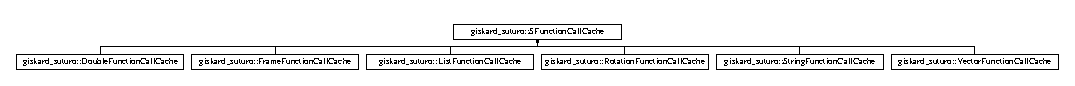
\includegraphics[height=0.712468cm]{structgiskard__suturo_1_1SFunctionCallCache}
\end{center}
\end{figure}
\subsection*{Public Member Functions}
\begin{DoxyCompactItemize}
\item 
\hypertarget{structgiskard__suturo_1_1SFunctionCallCache_a217492912917c2feff763d95642d06e9}{{\bfseries S\-Function\-Call\-Cache} (std\-::vector$<$ Spec\-Ptr $>$ \-\_\-arguments, Fn\-Def\-Ptr \-\_\-fn\-Def)}\label{structgiskard__suturo_1_1SFunctionCallCache_a217492912917c2feff763d95642d06e9}

\item 
Spec\-Ptr \hyperlink{structgiskard__suturo_1_1SFunctionCallCache_a311cb369df0c944afdbc525dd0c9d7b1}{create\-Instance} (Advanced\-Scope\-Ptr \&scope) const 
\end{DoxyCompactItemize}
\subsection*{Public Attributes}
\begin{DoxyCompactItemize}
\item 
std\-::vector$<$ Spec\-Ptr $>$ \hyperlink{structgiskard__suturo_1_1SFunctionCallCache_ad522b77747b469ad5c507f26dd6c74ae}{arguments}
\item 
Fn\-Def\-Ptr \hyperlink{structgiskard__suturo_1_1SFunctionCallCache_ab6e8b1ddb5c910291204be2de2d633df}{function\-Definition}
\end{DoxyCompactItemize}


\subsection{Detailed Description}
Base structure for caching function instances within function definitions. 

\subsection{Member Function Documentation}
\hypertarget{structgiskard__suturo_1_1SFunctionCallCache_a311cb369df0c944afdbc525dd0c9d7b1}{\index{giskard\-\_\-suturo\-::\-S\-Function\-Call\-Cache@{giskard\-\_\-suturo\-::\-S\-Function\-Call\-Cache}!create\-Instance@{create\-Instance}}
\index{create\-Instance@{create\-Instance}!giskard_suturo::SFunctionCallCache@{giskard\-\_\-suturo\-::\-S\-Function\-Call\-Cache}}
\subsubsection[{create\-Instance}]{\setlength{\rightskip}{0pt plus 5cm}Spec\-Ptr giskard\-\_\-suturo\-::\-S\-Function\-Call\-Cache\-::create\-Instance (
\begin{DoxyParamCaption}
\item[{Advanced\-Scope\-Ptr \&}]{scope}
\end{DoxyParamCaption}
) const\hspace{0.3cm}{\ttfamily [inline]}}}\label{structgiskard__suturo_1_1SFunctionCallCache_a311cb369df0c944afdbc525dd0c9d7b1}
Instantiates function call 

\subsection{Member Data Documentation}
\hypertarget{structgiskard__suturo_1_1SFunctionCallCache_ad522b77747b469ad5c507f26dd6c74ae}{\index{giskard\-\_\-suturo\-::\-S\-Function\-Call\-Cache@{giskard\-\_\-suturo\-::\-S\-Function\-Call\-Cache}!arguments@{arguments}}
\index{arguments@{arguments}!giskard_suturo::SFunctionCallCache@{giskard\-\_\-suturo\-::\-S\-Function\-Call\-Cache}}
\subsubsection[{arguments}]{\setlength{\rightskip}{0pt plus 5cm}std\-::vector$<$Spec\-Ptr$>$ giskard\-\_\-suturo\-::\-S\-Function\-Call\-Cache\-::arguments}}\label{structgiskard__suturo_1_1SFunctionCallCache_ad522b77747b469ad5c507f26dd6c74ae}
Arguments of the instance \hypertarget{structgiskard__suturo_1_1SFunctionCallCache_ab6e8b1ddb5c910291204be2de2d633df}{\index{giskard\-\_\-suturo\-::\-S\-Function\-Call\-Cache@{giskard\-\_\-suturo\-::\-S\-Function\-Call\-Cache}!function\-Definition@{function\-Definition}}
\index{function\-Definition@{function\-Definition}!giskard_suturo::SFunctionCallCache@{giskard\-\_\-suturo\-::\-S\-Function\-Call\-Cache}}
\subsubsection[{function\-Definition}]{\setlength{\rightskip}{0pt plus 5cm}Fn\-Def\-Ptr giskard\-\_\-suturo\-::\-S\-Function\-Call\-Cache\-::function\-Definition}}\label{structgiskard__suturo_1_1SFunctionCallCache_ab6e8b1ddb5c910291204be2de2d633df}
Function definition used for instancing 

The documentation for this struct was generated from the following file\-:\begin{DoxyCompactItemize}
\item 
giskard\-\_\-suturo\-\_\-parser/include/giskard\-\_\-suturo\-\_\-parser/functions.\-h\end{DoxyCompactItemize}

\hypertarget{structCollisionScene_1_1SQueryPoints}{\section{Collision\-Scene\-:\-:S\-Query\-Points Struct Reference}
\label{structCollisionScene_1_1SQueryPoints}\index{Collision\-Scene\-::\-S\-Query\-Points@{Collision\-Scene\-::\-S\-Query\-Points}}
}
\subsection*{Public Attributes}
\begin{DoxyCompactItemize}
\item 
\hypertarget{structCollisionScene_1_1SQueryPoints_ab1ea5365a8f6a1784b1ea3a954b4acb5}{Eigen\-::\-Vector3d {\bfseries on\-Link}}\label{structCollisionScene_1_1SQueryPoints_ab1ea5365a8f6a1784b1ea3a954b4acb5}

\item 
\hypertarget{structCollisionScene_1_1SQueryPoints_a2984d0e2f10e27354fdee9078de5f632}{Eigen\-::\-Vector3d {\bfseries in\-Scene}}\label{structCollisionScene_1_1SQueryPoints_a2984d0e2f10e27354fdee9078de5f632}

\end{DoxyCompactItemize}


The documentation for this struct was generated from the following file\-:\begin{DoxyCompactItemize}
\item 
suturo\-\_\-action\-\_\-server/include/suturo\-\_\-action\-\_\-server/Collision\-Scene.\-h\end{DoxyCompactItemize}

\hypertarget{structCollisionScene_1_1SRobotLink}{\section{Collision\-Scene\-:\-:S\-Robot\-Link Struct Reference}
\label{structCollisionScene_1_1SRobotLink}\index{Collision\-Scene\-::\-S\-Robot\-Link@{Collision\-Scene\-::\-S\-Robot\-Link}}
}
\subsection*{Public Attributes}
\begin{DoxyCompactItemize}
\item 
\hypertarget{structCollisionScene_1_1SRobotLink_ac4a672b5063c7f9fb0b28b0d25feafa8}{Eigen\-::\-Vector3d {\bfseries pos\-Bound}}\label{structCollisionScene_1_1SRobotLink_ac4a672b5063c7f9fb0b28b0d25feafa8}

\item 
\hypertarget{structCollisionScene_1_1SRobotLink_a302245e6caa88a6d1a8dec7a15a047e1}{Eigen\-::\-Vector3d {\bfseries neg\-Bound}}\label{structCollisionScene_1_1SRobotLink_a302245e6caa88a6d1a8dec7a15a047e1}

\end{DoxyCompactItemize}


The documentation for this struct was generated from the following file\-:\begin{DoxyCompactItemize}
\item 
suturo\-\_\-action\-\_\-server/include/suturo\-\_\-action\-\_\-server/Collision\-Scene.\-h\end{DoxyCompactItemize}

\hypertarget{classgiskard__suturo_1_1StringFunctionCallCache}{\section{giskard\-\_\-suturo\-:\-:String\-Function\-Call\-Cache Class Reference}
\label{classgiskard__suturo_1_1StringFunctionCallCache}\index{giskard\-\_\-suturo\-::\-String\-Function\-Call\-Cache@{giskard\-\_\-suturo\-::\-String\-Function\-Call\-Cache}}
}


Function call cache for string functions.  




{\ttfamily \#include $<$functions.\-h$>$}

Inheritance diagram for giskard\-\_\-suturo\-:\-:String\-Function\-Call\-Cache\-:\begin{figure}[H]
\begin{center}
\leavevmode
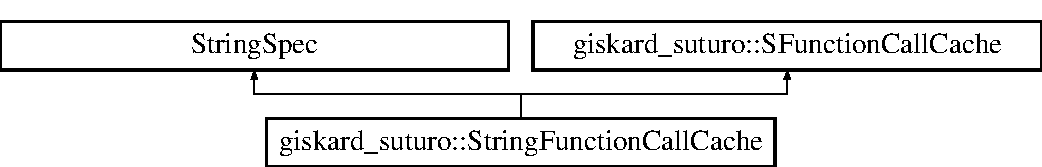
\includegraphics[height=2.000000cm]{classgiskard__suturo_1_1StringFunctionCallCache}
\end{center}
\end{figure}
\subsection*{Public Member Functions}
\begin{DoxyCompactItemize}
\item 
\hypertarget{classgiskard__suturo_1_1StringFunctionCallCache_a4c08e2104446b570b2cd8513b2a411dc}{{\bfseries String\-Function\-Call\-Cache} (std\-::vector$<$ Spec\-Ptr $>$ \-\_\-arguments, Fn\-Def\-Ptr \-\_\-fn\-Def)}\label{classgiskard__suturo_1_1StringFunctionCallCache_a4c08e2104446b570b2cd8513b2a411dc}

\item 
\hypertarget{classgiskard__suturo_1_1StringFunctionCallCache_ad9c1fd8cee7ba6bc28d5b5e13dca781d}{virtual bool {\bfseries equals} (const Spec \&other) const }\label{classgiskard__suturo_1_1StringFunctionCallCache_ad9c1fd8cee7ba6bc28d5b5e13dca781d}

\item 
\hypertarget{classgiskard__suturo_1_1StringFunctionCallCache_a363f8e53a181b7c5901314d620a3ff65}{void {\bfseries get\-\_\-input\-\_\-specs} (std\-::vector$<$ const Input\-Spec $\ast$ $>$ \&inputs) const }\label{classgiskard__suturo_1_1StringFunctionCallCache_a363f8e53a181b7c5901314d620a3ff65}

\item 
\hypertarget{classgiskard__suturo_1_1StringFunctionCallCache_a71c0149da10b3c112667440c0f02c4e1}{std\-::string {\bfseries get\-\_\-value} () const }\label{classgiskard__suturo_1_1StringFunctionCallCache_a71c0149da10b3c112667440c0f02c4e1}

\end{DoxyCompactItemize}
\subsection*{Additional Inherited Members}


\subsection{Detailed Description}
Function call cache for string functions. 

The documentation for this class was generated from the following file\-:\begin{DoxyCompactItemize}
\item 
giskard\-\_\-suturo\-\_\-parser/include/giskard\-\_\-suturo\-\_\-parser/functions.\-h\end{DoxyCompactItemize}

\hypertarget{classgiskard__suturo_1_1StringReferenceSpec}{\section{giskard\-\_\-suturo\-:\-:String\-Reference\-Spec Class Reference}
\label{classgiskard__suturo_1_1StringReferenceSpec}\index{giskard\-\_\-suturo\-::\-String\-Reference\-Spec@{giskard\-\_\-suturo\-::\-String\-Reference\-Spec}}
}


Reference for string scope variables.  




{\ttfamily \#include $<$specifications.\-h$>$}

Inheritance diagram for giskard\-\_\-suturo\-:\-:String\-Reference\-Spec\-:\begin{figure}[H]
\begin{center}
\leavevmode
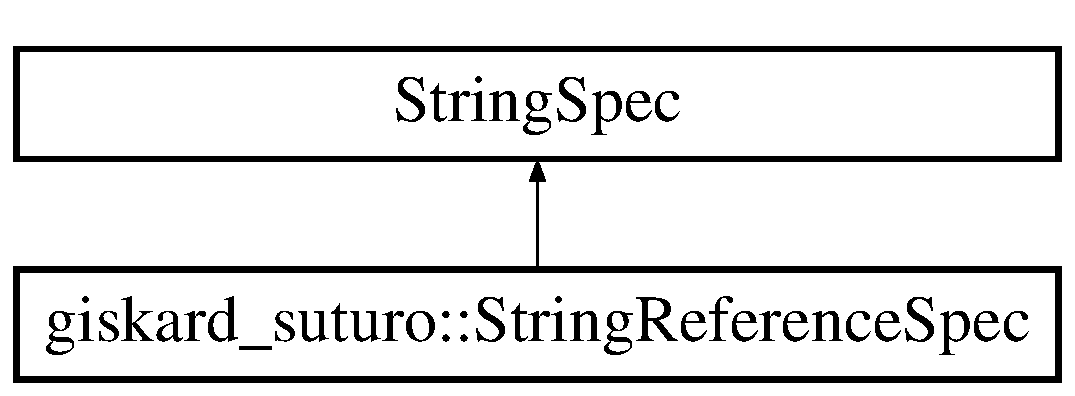
\includegraphics[height=2.000000cm]{classgiskard__suturo_1_1StringReferenceSpec}
\end{center}
\end{figure}
\subsection*{Public Member Functions}
\begin{DoxyCompactItemize}
\item 
\hypertarget{classgiskard__suturo_1_1StringReferenceSpec_a0ffe13b31aca247d93550ef38ae0dc45}{{\bfseries String\-Reference\-Spec} (const std\-::string \&ref\-Name, const boost\-::shared\-\_\-ptr$<$ \hyperlink{classgiskard__suturo_1_1AdvancedScope}{Advanced\-Scope} $>$ \&\-\_\-scope)}\label{classgiskard__suturo_1_1StringReferenceSpec_a0ffe13b31aca247d93550ef38ae0dc45}

\item 
\hypertarget{classgiskard__suturo_1_1StringReferenceSpec_a668f3ae9705593a495b5c34a2312edbe}{const std\-::string \& {\bfseries get\-\_\-reference\-\_\-name} () const }\label{classgiskard__suturo_1_1StringReferenceSpec_a668f3ae9705593a495b5c34a2312edbe}

\item 
\hypertarget{classgiskard__suturo_1_1StringReferenceSpec_aa0366c522078c2e1b5c1bb34b49ae1cd}{void {\bfseries set\-\_\-reference\-\_\-name} (const std\-::string \&ref\-Name)}\label{classgiskard__suturo_1_1StringReferenceSpec_aa0366c522078c2e1b5c1bb34b49ae1cd}

\item 
\hypertarget{classgiskard__suturo_1_1StringReferenceSpec_aaf53c5cfe15f9af75559a630deeeb243}{void {\bfseries get\-\_\-input\-\_\-specs} (std\-::vector$<$ const Input\-Spec $\ast$ $>$ \&inputs) const }\label{classgiskard__suturo_1_1StringReferenceSpec_aaf53c5cfe15f9af75559a630deeeb243}

\item 
\hypertarget{classgiskard__suturo_1_1StringReferenceSpec_ad12a39d9035a3ef022379811dad3a185}{bool {\bfseries equals} (const Spec \&other) const }\label{classgiskard__suturo_1_1StringReferenceSpec_ad12a39d9035a3ef022379811dad3a185}

\item 
\hypertarget{classgiskard__suturo_1_1StringReferenceSpec_a1352fc3b0b94ba2bd67fb3783368593d}{const boost\-::shared\-\_\-ptr\\*
$<$ \hyperlink{classgiskard__suturo_1_1AdvancedScope}{Advanced\-Scope} $>$ \& {\bfseries get\-Scope} () const }\label{classgiskard__suturo_1_1StringReferenceSpec_a1352fc3b0b94ba2bd67fb3783368593d}

\item 
\hypertarget{classgiskard__suturo_1_1StringReferenceSpec_a0b3dcced6e8bf4316a5e3a99c8b57647}{std\-::string {\bfseries get\-\_\-value} () const }\label{classgiskard__suturo_1_1StringReferenceSpec_a0b3dcced6e8bf4316a5e3a99c8b57647}

\end{DoxyCompactItemize}
\subsection*{Private Attributes}
\begin{DoxyCompactItemize}
\item 
\hypertarget{classgiskard__suturo_1_1StringReferenceSpec_a5efbdf748ce6210b092145e42c5319bc}{boost\-::shared\-\_\-ptr$<$ \hyperlink{classgiskard__suturo_1_1AdvancedScope}{Advanced\-Scope} $>$ {\bfseries scope}}\label{classgiskard__suturo_1_1StringReferenceSpec_a5efbdf748ce6210b092145e42c5319bc}

\item 
\hypertarget{classgiskard__suturo_1_1StringReferenceSpec_aa4eb4caee92c1f2348314ba82006c559}{std\-::string {\bfseries reference\-\_\-name}}\label{classgiskard__suturo_1_1StringReferenceSpec_aa4eb4caee92c1f2348314ba82006c559}

\end{DoxyCompactItemize}


\subsection{Detailed Description}
Reference for string scope variables. 

The documentation for this class was generated from the following files\-:\begin{DoxyCompactItemize}
\item 
giskard\-\_\-suturo\-\_\-parser/include/giskard\-\_\-suturo\-\_\-parser/specifications.\-h\item 
giskard\-\_\-suturo\-\_\-parser/src/specifications.\-cpp\end{DoxyCompactItemize}

\hypertarget{classSuturoSim_1_1SuturoSimPanel}{\section{Suturo\-Sim\-:\-:Suturo\-Sim\-Panel Class Reference}
\label{classSuturoSim_1_1SuturoSimPanel}\index{Suturo\-Sim\-::\-Suturo\-Sim\-Panel@{Suturo\-Sim\-::\-Suturo\-Sim\-Panel}}
}


!\-D\-E\-P\-R\-E\-C\-A\-T\-E\-D! Panel for setting up a simple scenario with interactive markers.  




{\ttfamily \#include $<$Suturo\-Sim\-Panel.\-h$>$}

Inheritance diagram for Suturo\-Sim\-:\-:Suturo\-Sim\-Panel\-:\begin{figure}[H]
\begin{center}
\leavevmode
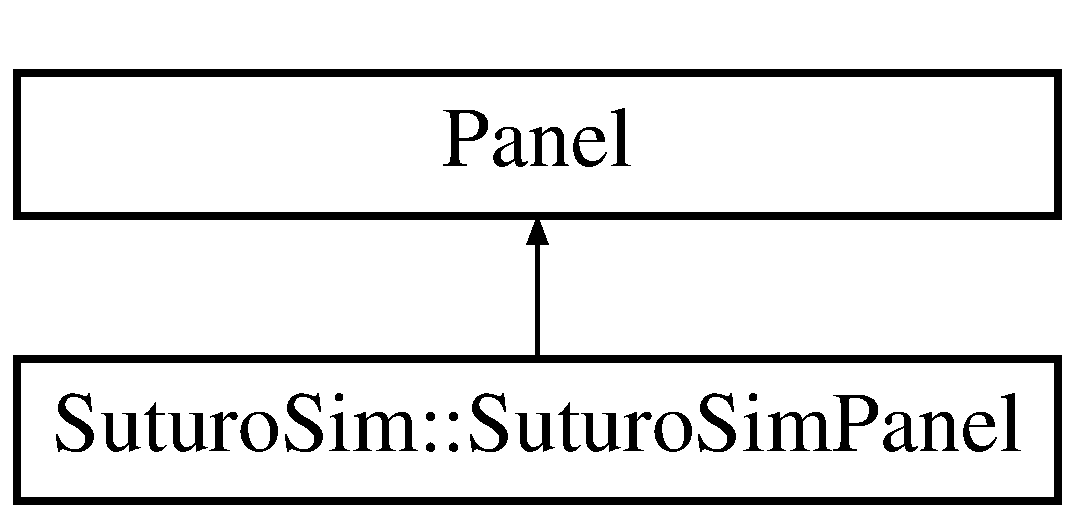
\includegraphics[height=2.000000cm]{classSuturoSim_1_1SuturoSimPanel}
\end{center}
\end{figure}
\subsection*{Public Slots}
\begin{DoxyCompactItemize}
\item 
\hypertarget{classSuturoSim_1_1SuturoSimPanel_a829172b8e0f903c6dd228c4d52f404e7}{void {\bfseries set\-Cmd\-Topic} (const Q\-String \&topic)}\label{classSuturoSim_1_1SuturoSimPanel_a829172b8e0f903c6dd228c4d52f404e7}

\item 
\hypertarget{classSuturoSim_1_1SuturoSimPanel_ad5e454d6a8da760db08473c10e544d4b}{void {\bfseries set\-Save\-Topic} (const Q\-String \&topic)}\label{classSuturoSim_1_1SuturoSimPanel_ad5e454d6a8da760db08473c10e544d4b}

\item 
\hypertarget{classSuturoSim_1_1SuturoSimPanel_a22e73d30da5c67efaa4e6d6bee8cbdc6}{void {\bfseries set\-Load\-Topic} (const Q\-String \&topic)}\label{classSuturoSim_1_1SuturoSimPanel_a22e73d30da5c67efaa4e6d6bee8cbdc6}

\item 
\hypertarget{classSuturoSim_1_1SuturoSimPanel_acc8be7f5d4f49254b56cc3e496a2d09e}{void {\bfseries create\-Object} ()}\label{classSuturoSim_1_1SuturoSimPanel_acc8be7f5d4f49254b56cc3e496a2d09e}

\item 
\hypertarget{classSuturoSim_1_1SuturoSimPanel_ade845c2f80c6a591b1d4613275a37170}{void {\bfseries load\-Scene} ()}\label{classSuturoSim_1_1SuturoSimPanel_ade845c2f80c6a591b1d4613275a37170}

\item 
\hypertarget{classSuturoSim_1_1SuturoSimPanel_a7a9c2ddd925123e67bd564b9d29941fd}{void {\bfseries save\-Scene} ()}\label{classSuturoSim_1_1SuturoSimPanel_a7a9c2ddd925123e67bd564b9d29941fd}

\item 
\hypertarget{classSuturoSim_1_1SuturoSimPanel_a3afb74a396bb5c08888685815f0b2e78}{void {\bfseries update\-Vis\-Marker} ()}\label{classSuturoSim_1_1SuturoSimPanel_a3afb74a396bb5c08888685815f0b2e78}

\end{DoxyCompactItemize}
\subsection*{Public Member Functions}
\begin{DoxyCompactItemize}
\item 
\hypertarget{classSuturoSim_1_1SuturoSimPanel_ac0c908bc97f767eb45964f9b7b7e49be}{{\bfseries Suturo\-Sim\-Panel} (Q\-Widget $\ast$parent=0)}\label{classSuturoSim_1_1SuturoSimPanel_ac0c908bc97f767eb45964f9b7b7e49be}

\item 
\hypertarget{classSuturoSim_1_1SuturoSimPanel_a914d811ad12b288ec3997217080c1cb1}{virtual void {\bfseries load} (const rviz\-::\-Config \&config)}\label{classSuturoSim_1_1SuturoSimPanel_a914d811ad12b288ec3997217080c1cb1}

\item 
\hypertarget{classSuturoSim_1_1SuturoSimPanel_ad5fd3fadcaefc12f0d6fda2fdb029c11}{virtual void {\bfseries save} (rviz\-::\-Config config) const }\label{classSuturoSim_1_1SuturoSimPanel_ad5fd3fadcaefc12f0d6fda2fdb029c11}

\item 
\hypertarget{classSuturoSim_1_1SuturoSimPanel_aebc9b3bbf9d91a9c9ad7ebf90ab16120}{virtual void {\bfseries on\-Initialize} ()}\label{classSuturoSim_1_1SuturoSimPanel_aebc9b3bbf9d91a9c9ad7ebf90ab16120}

\end{DoxyCompactItemize}
\subsection*{Protected Slots}
\begin{DoxyCompactItemize}
\item 
\hypertarget{classSuturoSim_1_1SuturoSimPanel_adbc55590d518d56ff3df2d68c8847d67}{void {\bfseries update\-Topic} ()}\label{classSuturoSim_1_1SuturoSimPanel_adbc55590d518d56ff3df2d68c8847d67}

\end{DoxyCompactItemize}
\subsection*{Protected Attributes}
\begin{DoxyCompactItemize}
\item 
\hypertarget{classSuturoSim_1_1SuturoSimPanel_af5a9f3dec16e3c08b6cb1d9eda39685e}{Q\-Line\-Edit $\ast$ {\bfseries sim\-Topic\-Widget}}\label{classSuturoSim_1_1SuturoSimPanel_af5a9f3dec16e3c08b6cb1d9eda39685e}

\item 
\hypertarget{classSuturoSim_1_1SuturoSimPanel_a8a9c5afb396021c44677cd6e06ecabbb}{Q\-String {\bfseries sim\-Topic}}\label{classSuturoSim_1_1SuturoSimPanel_a8a9c5afb396021c44677cd6e06ecabbb}

\item 
\hypertarget{classSuturoSim_1_1SuturoSimPanel_a339d97884ba83eba727e4889f6035bcb}{Q\-String {\bfseries save\-Topic}}\label{classSuturoSim_1_1SuturoSimPanel_a339d97884ba83eba727e4889f6035bcb}

\item 
\hypertarget{classSuturoSim_1_1SuturoSimPanel_a5f09de77557f41bbc8d59be30b9a2d40}{Q\-String {\bfseries load\-Topic}}\label{classSuturoSim_1_1SuturoSimPanel_a5f09de77557f41bbc8d59be30b9a2d40}

\item 
\hypertarget{classSuturoSim_1_1SuturoSimPanel_a9df78c29b9fe21dab33b4f69d7895a78}{Q\-V\-Box\-Layout $\ast$ {\bfseries marker\-Layout}}\label{classSuturoSim_1_1SuturoSimPanel_a9df78c29b9fe21dab33b4f69d7895a78}

\item 
\hypertarget{classSuturoSim_1_1SuturoSimPanel_afb406fd28df91352257761ce50d89da8}{visualization\-\_\-msgs\-::\-Marker {\bfseries vis\-Marker}}\label{classSuturoSim_1_1SuturoSimPanel_afb406fd28df91352257761ce50d89da8}

\item 
\hypertarget{classSuturoSim_1_1SuturoSimPanel_a9822f9eeb2995fde822fba70737217b7}{rviz\-::\-Property\-Tree\-Model $\ast$ {\bfseries obj\-P\-Tree}}\label{classSuturoSim_1_1SuturoSimPanel_a9822f9eeb2995fde822fba70737217b7}

\item 
\hypertarget{classSuturoSim_1_1SuturoSimPanel_a45609b7cf790afd6be44849ed1a9b6fa}{rviz\-::\-Property $\ast$ {\bfseries root\-Property}}\label{classSuturoSim_1_1SuturoSimPanel_a45609b7cf790afd6be44849ed1a9b6fa}

\item 
\hypertarget{classSuturoSim_1_1SuturoSimPanel_a9e8396c14ac7e2eaa8f1a45ed1656025}{rviz\-::\-String\-Property $\ast$ {\bfseries scene\-Path\-Property}}\label{classSuturoSim_1_1SuturoSimPanel_a9e8396c14ac7e2eaa8f1a45ed1656025}

\item 
\hypertarget{classSuturoSim_1_1SuturoSimPanel_a26e890475cd5cccff9bb01e9a8901fc3}{rviz\-::\-Property $\ast$ {\bfseries obj\-Root\-Property}}\label{classSuturoSim_1_1SuturoSimPanel_a26e890475cd5cccff9bb01e9a8901fc3}

\item 
\hypertarget{classSuturoSim_1_1SuturoSimPanel_a43094fb1217964f830dfbcc17eca4eef}{rviz\-::\-Property $\ast$ {\bfseries topics\-Property}}\label{classSuturoSim_1_1SuturoSimPanel_a43094fb1217964f830dfbcc17eca4eef}

\item 
\hypertarget{classSuturoSim_1_1SuturoSimPanel_ab5c583ad7a001af9e36fa6b91584090a}{rviz\-::\-Ros\-Topic\-Property $\ast$ {\bfseries sim\-Topic\-Property}}\label{classSuturoSim_1_1SuturoSimPanel_ab5c583ad7a001af9e36fa6b91584090a}

\item 
\hypertarget{classSuturoSim_1_1SuturoSimPanel_aa388c634f80a6fef039ed6bf7281ab25}{rviz\-::\-Ros\-Topic\-Property $\ast$ {\bfseries save\-Topic\-Property}}\label{classSuturoSim_1_1SuturoSimPanel_aa388c634f80a6fef039ed6bf7281ab25}

\item 
\hypertarget{classSuturoSim_1_1SuturoSimPanel_a01d13330615c72a4cfa9b9f4ee30780d}{rviz\-::\-Ros\-Topic\-Property $\ast$ {\bfseries load\-Topic\-Property}}\label{classSuturoSim_1_1SuturoSimPanel_a01d13330615c72a4cfa9b9f4ee30780d}

\item 
\hypertarget{classSuturoSim_1_1SuturoSimPanel_a4873e1ae2b5b27c5e24e6ac3b28155c3}{rviz\-::\-String\-Property $\ast$ {\bfseries obj\-Name\-Property}}\label{classSuturoSim_1_1SuturoSimPanel_a4873e1ae2b5b27c5e24e6ac3b28155c3}

\item 
\hypertarget{classSuturoSim_1_1SuturoSimPanel_a7fd40826beb684f0a831ab2e8f76b28d}{rviz\-::\-Tf\-Frame\-Property $\ast$ {\bfseries obj\-Frame\-Property}}\label{classSuturoSim_1_1SuturoSimPanel_a7fd40826beb684f0a831ab2e8f76b28d}

\item 
\hypertarget{classSuturoSim_1_1SuturoSimPanel_a1ae7af11c8ef48689b1e96e1fba6874f}{rviz\-::\-Color\-Property $\ast$ {\bfseries obj\-Color\-Property}}\label{classSuturoSim_1_1SuturoSimPanel_a1ae7af11c8ef48689b1e96e1fba6874f}

\item 
\hypertarget{classSuturoSim_1_1SuturoSimPanel_a2016a139b33ae8958a648151b977960c}{rviz\-::\-Float\-Property $\ast$ {\bfseries obj\-Alpha\-Property}}\label{classSuturoSim_1_1SuturoSimPanel_a2016a139b33ae8958a648151b977960c}

\item 
\hypertarget{classSuturoSim_1_1SuturoSimPanel_a2e198303dbb2c83e7c698a1e87c16a6f}{rviz\-::\-Enum\-Property $\ast$ {\bfseries obj\-Shape\-Property}}\label{classSuturoSim_1_1SuturoSimPanel_a2e198303dbb2c83e7c698a1e87c16a6f}

\item 
\hypertarget{classSuturoSim_1_1SuturoSimPanel_ae2ee7d7cc1606e7a2043d04a7d87de11}{rviz\-::\-Vector\-Property $\ast$ {\bfseries obj\-Scale\-Property}}\label{classSuturoSim_1_1SuturoSimPanel_ae2ee7d7cc1606e7a2043d04a7d87de11}

\item 
\hypertarget{classSuturoSim_1_1SuturoSimPanel_a25ae8435bf1b4ca52800a3b6cc76b546}{rviz\-::\-String\-Property $\ast$ {\bfseries obj\-Mesh\-Property}}\label{classSuturoSim_1_1SuturoSimPanel_a25ae8435bf1b4ca52800a3b6cc76b546}

\item 
\hypertarget{classSuturoSim_1_1SuturoSimPanel_ac549e5ed017709423354c018938544a8}{ros\-::\-Publisher {\bfseries sim\-Cmd\-Publisher}}\label{classSuturoSim_1_1SuturoSimPanel_ac549e5ed017709423354c018938544a8}

\item 
\hypertarget{classSuturoSim_1_1SuturoSimPanel_ab741354ff3940f6e77f03d485fffce57}{ros\-::\-Publisher {\bfseries sim\-Save\-Publisher}}\label{classSuturoSim_1_1SuturoSimPanel_ab741354ff3940f6e77f03d485fffce57}

\item 
\hypertarget{classSuturoSim_1_1SuturoSimPanel_a415fe204f39501d0a6ebbea0003792ea}{ros\-::\-Publisher {\bfseries sim\-Load\-Publisher}}\label{classSuturoSim_1_1SuturoSimPanel_a415fe204f39501d0a6ebbea0003792ea}

\item 
\hypertarget{classSuturoSim_1_1SuturoSimPanel_a7e36e472c99dbafe72c29743e538c3f5}{ros\-::\-Node\-Handle {\bfseries nh}}\label{classSuturoSim_1_1SuturoSimPanel_a7e36e472c99dbafe72c29743e538c3f5}

\end{DoxyCompactItemize}
\subsection*{Private Attributes}
\begin{DoxyCompactItemize}
\item 
\hypertarget{classSuturoSim_1_1SuturoSimPanel_a647938b22499afc53f92f3f1aeeb6d7c}{bool {\bfseries b\-Sim\-Cmd\-Connected}}\label{classSuturoSim_1_1SuturoSimPanel_a647938b22499afc53f92f3f1aeeb6d7c}

\item 
\hypertarget{classSuturoSim_1_1SuturoSimPanel_acf053b45869d3002a00ffa05e8996fbf}{bool {\bfseries b\-Sim\-Save\-Connected}}\label{classSuturoSim_1_1SuturoSimPanel_acf053b45869d3002a00ffa05e8996fbf}

\item 
\hypertarget{classSuturoSim_1_1SuturoSimPanel_a4a596323456c86139192c4697194fb18}{bool {\bfseries b\-Sim\-Load\-Connected}}\label{classSuturoSim_1_1SuturoSimPanel_a4a596323456c86139192c4697194fb18}

\end{DoxyCompactItemize}


\subsection{Detailed Description}
!\-D\-E\-P\-R\-E\-C\-A\-T\-E\-D! Panel for setting up a simple scenario with interactive markers. 

The documentation for this class was generated from the following files\-:\begin{DoxyCompactItemize}
\item 
suturo\-\_\-action\-\_\-tester/include/suturo\-\_\-action\-\_\-tester/Suturo\-Sim\-Panel.\-h\item 
suturo\-\_\-action\-\_\-tester/src/Suturo\-Sim\-Panel.\-cpp\end{DoxyCompactItemize}

\hypertarget{structTFQuery}{\section{T\-F\-Query Struct Reference}
\label{structTFQuery}\index{T\-F\-Query@{T\-F\-Query}}
}


Query looking up a transformation in Tf.  




{\ttfamily \#include $<$Giskard\-Action\-Server.\-h$>$}

Inheritance diagram for T\-F\-Query\-:\begin{figure}[H]
\begin{center}
\leavevmode
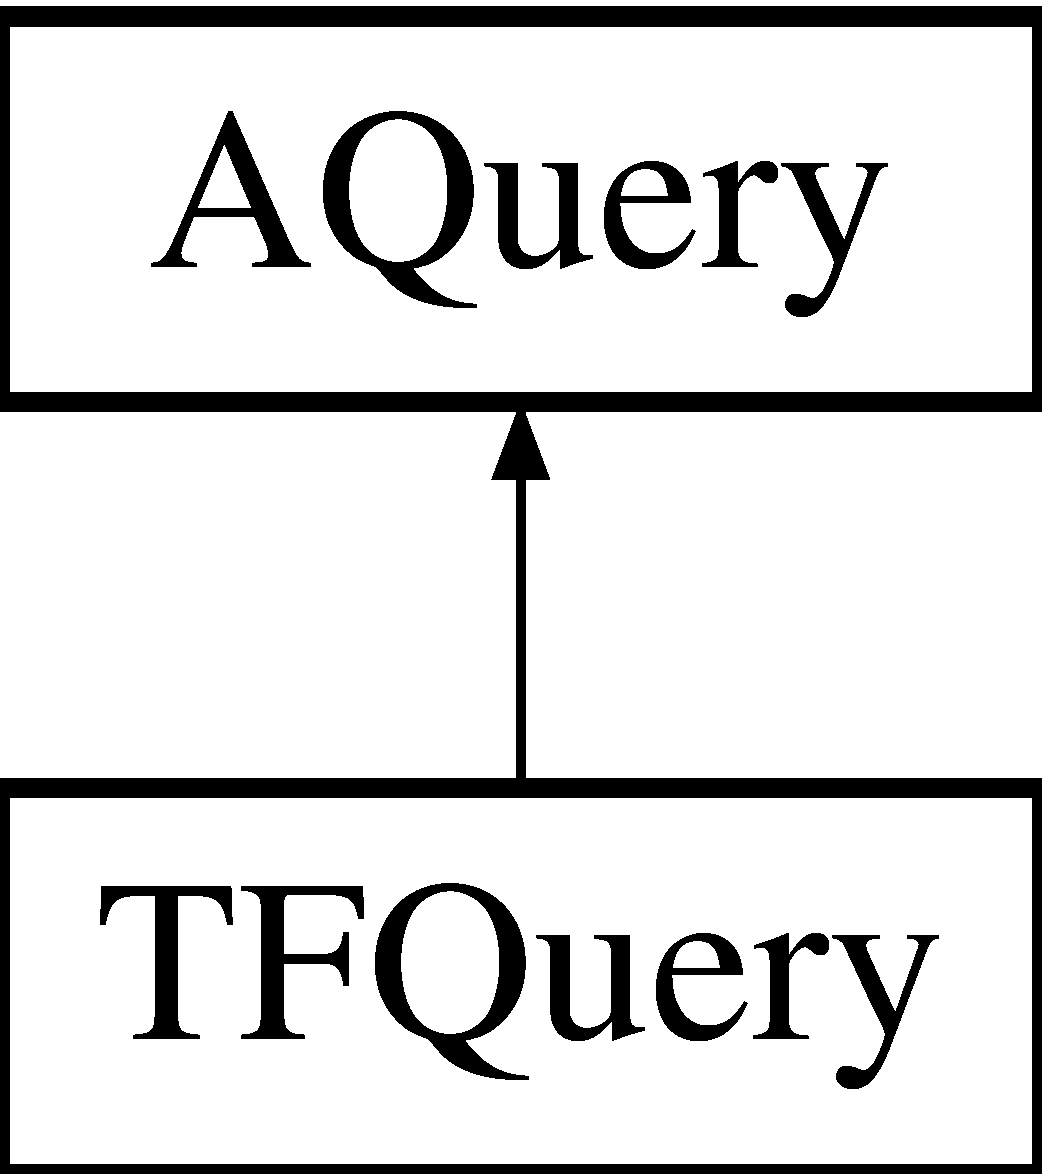
\includegraphics[height=2.000000cm]{structTFQuery}
\end{center}
\end{figure}
\subsection*{Public Member Functions}
\begin{DoxyCompactItemize}
\item 
\hypertarget{structTFQuery_a065412ea50cfcbab8fde438e6dce7d0d}{{\bfseries T\-F\-Query} (\hyperlink{classGiskardActionServer}{Giskard\-Action\-Server} $\ast$p\-S, string \hyperlink{structAQuery_a209eec59fbdf038ec7de39db059ddaa4}{name}, string target\-Frame, string source\-Frame, tf\-::\-Transform\-Listener $\ast$\-\_\-tf\-Listener)}\label{structTFQuery_a065412ea50cfcbab8fde438e6dce7d0d}

\item 
\hypertarget{structTFQuery_aa666ac37934e7e3291bf45094dde9aa2}{bool {\bfseries eval} ()}\label{structTFQuery_aa666ac37934e7e3291bf45094dde9aa2}

\end{DoxyCompactItemize}
\subsection*{Private Attributes}
\begin{DoxyCompactItemize}
\item 
const string \hyperlink{structTFQuery_a1827c7ca85239f98da28cb9bebf630bb}{frame\-Id}
\item 
const string \hyperlink{structTFQuery_aa5198bb657f18acf54ca14f5f2e77728}{ref\-Frame}
\item 
const tf\-::\-Transform\-Listener $\ast$ \hyperlink{structTFQuery_af963e7f338115d80baa86aeea7bd7570}{tf\-Listener}
\end{DoxyCompactItemize}
\subsection*{Additional Inherited Members}


\subsection{Detailed Description}
Query looking up a transformation in Tf. 

\subsection{Member Data Documentation}
\hypertarget{structTFQuery_a1827c7ca85239f98da28cb9bebf630bb}{\index{T\-F\-Query@{T\-F\-Query}!frame\-Id@{frame\-Id}}
\index{frame\-Id@{frame\-Id}!TFQuery@{T\-F\-Query}}
\subsubsection[{frame\-Id}]{\setlength{\rightskip}{0pt plus 5cm}const string T\-F\-Query\-::frame\-Id\hspace{0.3cm}{\ttfamily [private]}}}\label{structTFQuery_a1827c7ca85239f98da28cb9bebf630bb}
Target frame \hypertarget{structTFQuery_aa5198bb657f18acf54ca14f5f2e77728}{\index{T\-F\-Query@{T\-F\-Query}!ref\-Frame@{ref\-Frame}}
\index{ref\-Frame@{ref\-Frame}!TFQuery@{T\-F\-Query}}
\subsubsection[{ref\-Frame}]{\setlength{\rightskip}{0pt plus 5cm}const string T\-F\-Query\-::ref\-Frame\hspace{0.3cm}{\ttfamily [private]}}}\label{structTFQuery_aa5198bb657f18acf54ca14f5f2e77728}
Source frame \hypertarget{structTFQuery_af963e7f338115d80baa86aeea7bd7570}{\index{T\-F\-Query@{T\-F\-Query}!tf\-Listener@{tf\-Listener}}
\index{tf\-Listener@{tf\-Listener}!TFQuery@{T\-F\-Query}}
\subsubsection[{tf\-Listener}]{\setlength{\rightskip}{0pt plus 5cm}const tf\-::\-Transform\-Listener$\ast$ T\-F\-Query\-::tf\-Listener\hspace{0.3cm}{\ttfamily [private]}}}\label{structTFQuery_af963e7f338115d80baa86aeea7bd7570}
Pointer to transform listener used for lookup 

The documentation for this struct was generated from the following file\-:\begin{DoxyCompactItemize}
\item 
suturo\-\_\-action\-\_\-server/include/suturo\-\_\-action\-\_\-server/Giskard\-Action\-Server.\-h\end{DoxyCompactItemize}

\hypertarget{structVector3f}{\section{Vector3f Struct Reference}
\label{structVector3f}\index{Vector3f@{Vector3f}}
}
\subsection*{Public Member Functions}
\begin{DoxyCompactItemize}
\item 
\hypertarget{structVector3f_a727fefc00986bbca1f0493d6731d4064}{C\-U\-D\-A\-\_\-\-C\-A\-L\-L\-A\-B\-L\-E\-\_\-\-M\-E\-M\-B\-E\-R {\bfseries Vector3f} (float x, float y, float z)}\label{structVector3f_a727fefc00986bbca1f0493d6731d4064}

\item 
\hypertarget{structVector3f_a9048708044970abfaedd9d3659434371}{C\-U\-D\-A\-\_\-\-C\-A\-L\-L\-A\-B\-L\-E\-\_\-\-M\-E\-M\-B\-E\-R \hyperlink{structVector3f}{Vector3f} {\bfseries cross} (\hyperlink{structVector3f}{Vector3f} v) const }\label{structVector3f_a9048708044970abfaedd9d3659434371}

\item 
\hypertarget{structVector3f_ab781ea4785ff76b1d942dc2dff32d87e}{C\-U\-D\-A\-\_\-\-C\-A\-L\-L\-A\-B\-L\-E\-\_\-\-M\-E\-M\-B\-E\-R float {\bfseries norm} () const }\label{structVector3f_ab781ea4785ff76b1d942dc2dff32d87e}

\end{DoxyCompactItemize}
\subsection*{Public Attributes}
\begin{DoxyCompactItemize}
\item 
\hypertarget{structVector3f_a4aca0751716b7099b397e8c63b16bfcf}{float {\bfseries x}}\label{structVector3f_a4aca0751716b7099b397e8c63b16bfcf}

\item 
\hypertarget{structVector3f_a8a602e2ee75126feb520c2aa27e7eff5}{float {\bfseries y}}\label{structVector3f_a8a602e2ee75126feb520c2aa27e7eff5}

\item 
\hypertarget{structVector3f_a470cff51eb6463672be518f5af4e26db}{float {\bfseries z}}\label{structVector3f_a470cff51eb6463672be518f5af4e26db}

\end{DoxyCompactItemize}


The documentation for this struct was generated from the following file\-:\begin{DoxyCompactItemize}
\item 
suturo\-\_\-action\-\_\-server/include/suturo\-\_\-action\-\_\-server/Vector3f.\-h\end{DoxyCompactItemize}

\hypertarget{classgiskard__suturo_1_1VectorFunctionCallCache}{\section{giskard\-\_\-suturo\-:\-:Vector\-Function\-Call\-Cache Class Reference}
\label{classgiskard__suturo_1_1VectorFunctionCallCache}\index{giskard\-\_\-suturo\-::\-Vector\-Function\-Call\-Cache@{giskard\-\_\-suturo\-::\-Vector\-Function\-Call\-Cache}}
}


Function call cache for vector functions.  




{\ttfamily \#include $<$functions.\-h$>$}

Inheritance diagram for giskard\-\_\-suturo\-:\-:Vector\-Function\-Call\-Cache\-:\begin{figure}[H]
\begin{center}
\leavevmode
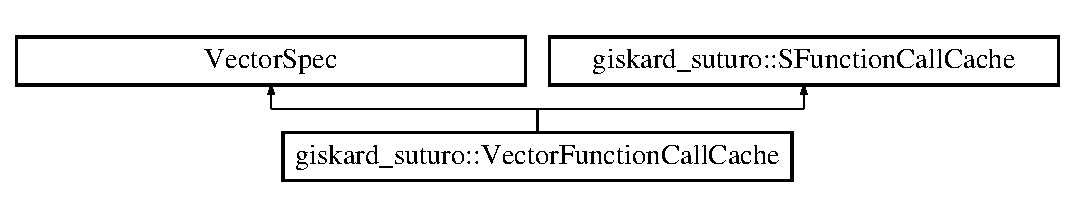
\includegraphics[height=2.000000cm]{classgiskard__suturo_1_1VectorFunctionCallCache}
\end{center}
\end{figure}
\subsection*{Public Member Functions}
\begin{DoxyCompactItemize}
\item 
\hypertarget{classgiskard__suturo_1_1VectorFunctionCallCache_a53d433daeb65d992e5e86029ccf7a1ee}{{\bfseries Vector\-Function\-Call\-Cache} (std\-::vector$<$ Spec\-Ptr $>$ \-\_\-arguments, Fn\-Def\-Ptr \-\_\-fn\-Def)}\label{classgiskard__suturo_1_1VectorFunctionCallCache_a53d433daeb65d992e5e86029ccf7a1ee}

\item 
\hypertarget{classgiskard__suturo_1_1VectorFunctionCallCache_a633ebfe8ddb9b0fffa9c8fa05ca1938e}{virtual bool {\bfseries equals} (const Spec \&other) const }\label{classgiskard__suturo_1_1VectorFunctionCallCache_a633ebfe8ddb9b0fffa9c8fa05ca1938e}

\item 
\hypertarget{classgiskard__suturo_1_1VectorFunctionCallCache_a5dfd205ece902e4a56fb5b30639b2b2b}{void {\bfseries get\-\_\-input\-\_\-specs} (std\-::vector$<$ const Input\-Spec $\ast$ $>$ \&inputs) const }\label{classgiskard__suturo_1_1VectorFunctionCallCache_a5dfd205ece902e4a56fb5b30639b2b2b}

\item 
\hypertarget{classgiskard__suturo_1_1VectorFunctionCallCache_a77a720a3ada6e2c43ce35c962def3302}{K\-D\-L\-::\-Expression$<$ K\-D\-L\-::\-Vector $>$\-::Ptr {\bfseries get\-\_\-expression} (const giskard\-\_\-core\-::\-Scope \&scope)}\label{classgiskard__suturo_1_1VectorFunctionCallCache_a77a720a3ada6e2c43ce35c962def3302}

\end{DoxyCompactItemize}
\subsection*{Additional Inherited Members}


\subsection{Detailed Description}
Function call cache for vector functions. 

The documentation for this class was generated from the following file\-:\begin{DoxyCompactItemize}
\item 
giskard\-\_\-suturo\-\_\-parser/include/giskard\-\_\-suturo\-\_\-parser/functions.\-h\end{DoxyCompactItemize}

\hypertarget{classVisualizationManager}{\section{Visualization\-Manager Class Reference}
\label{classVisualizationManager}\index{Visualization\-Manager@{Visualization\-Manager}}
}


Class allowing a visualization supporting a frame like update style.  




{\ttfamily \#include $<$Visualization\-Manager.\-h$>$}

\subsection*{Public Member Functions}
\begin{DoxyCompactItemize}
\item 
void \hyperlink{classVisualizationManager_ac0c108a709de3c89db8c43707dd2220a}{add\-Namespace} (int ns, string name)
\begin{DoxyCompactList}\small\item\em Add a namespace. \end{DoxyCompactList}\item 
void \hyperlink{classVisualizationManager_abc61da41f78114714fa3c58de96d66eb}{clear\-Marker\-N\-S} (int ns, ros\-::\-Publisher $\ast$publisher)
\begin{DoxyCompactList}\small\item\em Clear all markers within a namespace. \end{DoxyCompactList}\item 
void \hyperlink{classVisualizationManager_a8d712fe1e6c7743100a1ba7fa019a781}{clear\-All\-Markers} (ros\-::\-Publisher $\ast$publisher)
\begin{DoxyCompactList}\small\item\em Delete all markers managed by this manager. \end{DoxyCompactList}\item 
\hypertarget{classVisualizationManager_a831e69c1d56167c0d02ab4841d6d7bc5}{void \hyperlink{classVisualizationManager_a831e69c1d56167c0d02ab4841d6d7bc5}{begin\-New\-Draw\-Cycle} ()}\label{classVisualizationManager_a831e69c1d56167c0d02ab4841d6d7bc5}

\begin{DoxyCompactList}\small\item\em Begin a new draw cycle. \end{DoxyCompactList}\item 
void \hyperlink{classVisualizationManager_adeeb76e606e872e17984fb372ee295ad}{end\-Draw\-Cycle} (vector$<$ visualization\-\_\-msgs\-::\-Marker $>$ \&vis)
\begin{DoxyCompactList}\small\item\em End the current draw cycle and append delete commands to marker array. \end{DoxyCompactList}\item 
visualization\-\_\-msgs\-::\-Marker \hyperlink{classVisualizationManager_aebf5df7c638e1ecf0cc3bacde43c615e}{trail\-Marker} (int ns, const vector$<$ Vector3d $>$ \&points, double width=0.\-1, float r=0.f, float g=1.f, float b=0.f, float a=1.f, string frame\-\_\-id=\char`\"{}odom\-\_\-combined\char`\"{})
\begin{DoxyCompactList}\small\item\em Creates a trail marker from an array of points. \end{DoxyCompactList}\item 
visualization\-\_\-msgs\-::\-Marker \hyperlink{classVisualizationManager_a9c99686f3418df6a11e10e8f59ba7c4d}{shape\-Marker} (int ns, Affine3d pose, int shape, Vector3d size, float r=0.f, float g=1.f, float b=0.f, float a=1.f, string frame\-\_\-id=\char`\"{}odom\-\_\-combined\char`\"{})
\begin{DoxyCompactList}\small\item\em Creates a marker with an arbitrary shape. \end{DoxyCompactList}\item 
visualization\-\_\-msgs\-::\-Marker \hyperlink{classVisualizationManager_a1b5d2724fb4d8520936b9be6e8b58e55}{sphere\-Marker} (int ns, Vector3d center, double radius, float r=1.f, float g=1.f, float b=1.f, float a=1.f, string frame\-\_\-id=\char`\"{}odom\-\_\-combined\char`\"{})
\begin{DoxyCompactList}\small\item\em Creates a spherical marker. \end{DoxyCompactList}\item 
visualization\-\_\-msgs\-::\-Marker \hyperlink{classVisualizationManager_a470dca284f28b0884053b7e02550ff3a}{vector\-Marker} (int ns, Vector3d pos, Vector3d vector, float r=1.f, float g=1.f, float b=1.f, float a=1.f, double width=0.\-01, double head\-Width=0.\-02, string frame\-\_\-id=\char`\"{}odom\-\_\-combined\char`\"{})
\begin{DoxyCompactList}\small\item\em Creates an arrow marker visualizing a vector as direction. \end{DoxyCompactList}\item 
visualization\-\_\-msgs\-::\-Marker \hyperlink{classVisualizationManager_a58d47a4507c3216b906a166c9cc1ba17}{arrow\-Marker} (int ns, Vector3d start, Vector3d end, float r=1.f, float g=1.f, float b=1.f, float a=1.f, double width=0.\-01, double head\-Width=0.\-02, string frame\-\_\-id=\char`\"{}odom\-\_\-combined\char`\"{})
\begin{DoxyCompactList}\small\item\em Creates an arrow marker connecting two points. \end{DoxyCompactList}\item 
visualization\-\_\-msgs\-::\-Marker \hyperlink{classVisualizationManager_a16a80f780d1ab0b450be70aa14ba09b2}{text\-Marker} (int ns, Vector3d pos, string text, float r=1.f, float g=1.f, float b=1.f, float a=1.f, double height=0.\-015, string frame\-\_\-id=\char`\"{}odom\-\_\-combined\char`\"{})
\begin{DoxyCompactList}\small\item\em Creates a text marker. \end{DoxyCompactList}\item 
void \hyperlink{classVisualizationManager_a37a6fc1245fe6ed7f3410792cf41e7ec}{annotated\-Vector} (vector$<$ visualization\-\_\-msgs\-::\-Marker $>$ \&array, int ns, Vector3d pos, Vector3d vector, string text, float r=1.f, float g=1.f, float b=1.f, float a=1.f, string frame\-\_\-id=\char`\"{}odom\-\_\-combined\char`\"{})
\begin{DoxyCompactList}\small\item\em Creates a vector with a label. \end{DoxyCompactList}\item 
void \hyperlink{classVisualizationManager_a9724369385e07346cf0d07dd57d66458}{annotated\-Point} (vector$<$ visualization\-\_\-msgs\-::\-Marker $>$ \&array, int ns, Vector3d pos, string text, float r=1.f, float g=1.f, float b=1.f, float a=1.f, string frame\-\_\-id=\char`\"{}odom\-\_\-combined\char`\"{})
\begin{DoxyCompactList}\small\item\em Creates a point with a label. \end{DoxyCompactList}\item 
void \hyperlink{classVisualizationManager_a9caff4d805416c67cc7fb3250259abe0}{pose\-Marker} (vector$<$ visualization\-\_\-msgs\-::\-Marker $>$ \&array, int ns, Affine3d pose, double arrow\-Length=0.\-1, float a=1.f, string frame\-\_\-id=\char`\"{}odom\-\_\-combined\char`\"{})
\begin{DoxyCompactList}\small\item\em Creates a marker visualizing a pose as coordinate axes. \end{DoxyCompactList}\item 
visualization\-\_\-msgs\-::\-Marker \hyperlink{classVisualizationManager_a53193705b968d8ef4bc87ca7b44ba597}{mesh\-Marker} (int ns, Affine3d pose, Vector3d scale, string resource, string frame\-\_\-id=\char`\"{}odom\-\_\-combined\char`\"{}, Vector4f color=Vector4f\-::\-Zero())
\begin{DoxyCompactList}\small\item\em Creates a mesh marker using a U\-R\-I. \end{DoxyCompactList}\item 
visualization\-\_\-msgs\-::\-Marker \hyperlink{classVisualizationManager_aa6726def2fb09cfd32517eb474693046}{mesh\-Marker} (int ns, Affine3d pose, Vector3d scale, string resource, string frame\-\_\-id=\char`\"{}odom\-\_\-combined\char`\"{}, float r=0, float g=0, float b=0, float a=0)
\begin{DoxyCompactList}\small\item\em \{ function\-\_\-description \} \end{DoxyCompactList}\item 
int \hyperlink{classVisualizationManager_ab5f80d32ca698923cce675d79289c262}{consume\-Id} (int ns)
\begin{DoxyCompactList}\small\item\em Manually get the next available Id for a namespace. \end{DoxyCompactList}\item 
string \hyperlink{classVisualizationManager_a5d0d1765b3f64a3a542ca93c46674ce3}{get\-Namespace} (int ns)
\begin{DoxyCompactList}\small\item\em Gets the readable name of a namespace. \end{DoxyCompactList}\end{DoxyCompactItemize}
\subsection*{Private Member Functions}
\begin{DoxyCompactItemize}
\item 
geometry\-\_\-msgs\-::\-Point \hyperlink{classVisualizationManager_aeeccb0e2791c358741fa5124535141e5}{vec2\-Point} (Vector3d vec)
\begin{DoxyCompactList}\small\item\em Internal function to convert vectors to point messages. \end{DoxyCompactList}\item 
geometry\-\_\-msgs\-::\-Quaternion \hyperlink{classVisualizationManager_a0477cd745c1b09d67dbe2b850bd52e46}{quat2\-Quat\-Msg} (Quaterniond quat)
\begin{DoxyCompactList}\small\item\em Internal function to convert Quaternions to Quaternion messages. \end{DoxyCompactList}\end{DoxyCompactItemize}
\subsection*{Private Attributes}
\begin{DoxyCompactItemize}
\item 
map$<$ int, string $>$ \hyperlink{classVisualizationManager_a73b79150d1efd76f132313088b99f172}{namespaces}
\item 
map$<$ int, int $>$ \hyperlink{classVisualizationManager_a043ed969cfc739b44ff494c04fa2dbab}{ids}
\item 
map$<$ int, int $>$ \hyperlink{classVisualizationManager_a0a7d5e6613a54f37fefb6c4322ec434a}{last\-Ids}
\end{DoxyCompactItemize}


\subsection{Detailed Description}
Class allowing a visualization supporting a frame like update style. 

The visualization manager manages namespaces and marker Ids automatically. It can be used to draw in frames, e.\-g. start a frame, draw markers, end frame. The markers of the previous frame are automatically deleted. 

\subsection{Member Function Documentation}
\hypertarget{classVisualizationManager_ac0c108a709de3c89db8c43707dd2220a}{\index{Visualization\-Manager@{Visualization\-Manager}!add\-Namespace@{add\-Namespace}}
\index{add\-Namespace@{add\-Namespace}!VisualizationManager@{Visualization\-Manager}}
\subsubsection[{add\-Namespace}]{\setlength{\rightskip}{0pt plus 5cm}void Visualization\-Manager\-::add\-Namespace (
\begin{DoxyParamCaption}
\item[{int}]{ns, }
\item[{string}]{name}
\end{DoxyParamCaption}
)}}\label{classVisualizationManager_ac0c108a709de3c89db8c43707dd2220a}


Add a namespace. 


\begin{DoxyParams}[1]{Parameters}
\mbox{\tt in}  & {\em ns} & The Id of the namespace \\
\hline
\mbox{\tt in}  & {\em name} & The readable name of the namespace \\
\hline
\end{DoxyParams}
\hypertarget{classVisualizationManager_a9724369385e07346cf0d07dd57d66458}{\index{Visualization\-Manager@{Visualization\-Manager}!annotated\-Point@{annotated\-Point}}
\index{annotated\-Point@{annotated\-Point}!VisualizationManager@{Visualization\-Manager}}
\subsubsection[{annotated\-Point}]{\setlength{\rightskip}{0pt plus 5cm}void Visualization\-Manager\-::annotated\-Point (
\begin{DoxyParamCaption}
\item[{vector$<$ visualization\-\_\-msgs\-::\-Marker $>$ \&}]{array, }
\item[{int}]{ns, }
\item[{Vector3d}]{pos, }
\item[{string}]{text, }
\item[{float}]{r = {\ttfamily 1.f}, }
\item[{float}]{g = {\ttfamily 1.f}, }
\item[{float}]{b = {\ttfamily 1.f}, }
\item[{float}]{a = {\ttfamily 1.f}, }
\item[{string}]{frame\-\_\-id = {\ttfamily \char`\"{}odom\-\_\-combined\char`\"{}}}
\end{DoxyParamCaption}
)}}\label{classVisualizationManager_a9724369385e07346cf0d07dd57d66458}


Creates a point with a label. 


\begin{DoxyParams}[1]{Parameters}
 & {\em array} & Marker array to add the markers to \\
\hline
\mbox{\tt in}  & {\em ns} & Namespace to add the marker to \\
\hline
\mbox{\tt in}  & {\em pos} & Position of the point \\
\hline
\mbox{\tt in}  & {\em text} & Text of the label \\
\hline
\mbox{\tt in}  & {\em r} & Marker color\-: Red \\
\hline
\mbox{\tt in}  & {\em g} & Marker color\-: Green \\
\hline
\mbox{\tt in}  & {\em b} & Marker color\-: Blue \\
\hline
\mbox{\tt in}  & {\em a} & Marker color\-: Alpha \\
\hline
\mbox{\tt in}  & {\em frame\-\_\-id} & Reference frame for the marker \\
\hline
\end{DoxyParams}
\hypertarget{classVisualizationManager_a37a6fc1245fe6ed7f3410792cf41e7ec}{\index{Visualization\-Manager@{Visualization\-Manager}!annotated\-Vector@{annotated\-Vector}}
\index{annotated\-Vector@{annotated\-Vector}!VisualizationManager@{Visualization\-Manager}}
\subsubsection[{annotated\-Vector}]{\setlength{\rightskip}{0pt plus 5cm}void Visualization\-Manager\-::annotated\-Vector (
\begin{DoxyParamCaption}
\item[{vector$<$ visualization\-\_\-msgs\-::\-Marker $>$ \&}]{array, }
\item[{int}]{ns, }
\item[{Vector3d}]{pos, }
\item[{Vector3d}]{vector, }
\item[{string}]{text, }
\item[{float}]{r = {\ttfamily 1.f}, }
\item[{float}]{g = {\ttfamily 1.f}, }
\item[{float}]{b = {\ttfamily 1.f}, }
\item[{float}]{a = {\ttfamily 1.f}, }
\item[{string}]{frame\-\_\-id = {\ttfamily \char`\"{}odom\-\_\-combined\char`\"{}}}
\end{DoxyParamCaption}
)}}\label{classVisualizationManager_a37a6fc1245fe6ed7f3410792cf41e7ec}


Creates a vector with a label. 


\begin{DoxyParams}[1]{Parameters}
 & {\em array} & Marker array to add the markers to \\
\hline
\mbox{\tt in}  & {\em ns} & Namespace to add the marker to \\
\hline
\mbox{\tt in}  & {\em pos} & Position of the base of the arrow \\
\hline
\mbox{\tt in}  & {\em vector} & Vector to visualize \\
\hline
\mbox{\tt in}  & {\em text} & The text \\
\hline
\mbox{\tt in}  & {\em r} & Marker color\-: Red \\
\hline
\mbox{\tt in}  & {\em g} & Marker color\-: Green \\
\hline
\mbox{\tt in}  & {\em b} & Marker color\-: Blue \\
\hline
\mbox{\tt in}  & {\em a} & Marker color\-: Alpha \\
\hline
\mbox{\tt in}  & {\em frame\-\_\-id} & Reference frame for the marker \\
\hline
\end{DoxyParams}
\hypertarget{classVisualizationManager_a58d47a4507c3216b906a166c9cc1ba17}{\index{Visualization\-Manager@{Visualization\-Manager}!arrow\-Marker@{arrow\-Marker}}
\index{arrow\-Marker@{arrow\-Marker}!VisualizationManager@{Visualization\-Manager}}
\subsubsection[{arrow\-Marker}]{\setlength{\rightskip}{0pt plus 5cm}visualization\-\_\-msgs\-::\-Marker Visualization\-Manager\-::arrow\-Marker (
\begin{DoxyParamCaption}
\item[{int}]{ns, }
\item[{Vector3d}]{start, }
\item[{Vector3d}]{end, }
\item[{float}]{r = {\ttfamily 1.f}, }
\item[{float}]{g = {\ttfamily 1.f}, }
\item[{float}]{b = {\ttfamily 1.f}, }
\item[{float}]{a = {\ttfamily 1.f}, }
\item[{double}]{width = {\ttfamily 0.01}, }
\item[{double}]{head\-Width = {\ttfamily 0.02}, }
\item[{string}]{frame\-\_\-id = {\ttfamily \char`\"{}odom\-\_\-combined\char`\"{}}}
\end{DoxyParamCaption}
)}}\label{classVisualizationManager_a58d47a4507c3216b906a166c9cc1ba17}


Creates an arrow marker connecting two points. 


\begin{DoxyParams}[1]{Parameters}
\mbox{\tt in}  & {\em ns} & Namespace to add the marker to \\
\hline
\mbox{\tt in}  & {\em start} & Starting point \\
\hline
\mbox{\tt in}  & {\em end} & End point \\
\hline
\mbox{\tt in}  & {\em r} & Marker color\-: Red \\
\hline
\mbox{\tt in}  & {\em g} & Marker color\-: Green \\
\hline
\mbox{\tt in}  & {\em b} & Marker color\-: Blue \\
\hline
\mbox{\tt in}  & {\em a} & Marker color\-: Alpha \\
\hline
\mbox{\tt in}  & {\em width} & Width of the arrow \\
\hline
\mbox{\tt in}  & {\em head\-Width} & Width of the arrowhead \\
\hline
\mbox{\tt in}  & {\em frame\-\_\-id} & Reference frame for the marker\\
\hline
\end{DoxyParams}
\begin{DoxyReturn}{Returns}
Arrow marker connecting start and end point 
\end{DoxyReturn}
\hypertarget{classVisualizationManager_a8d712fe1e6c7743100a1ba7fa019a781}{\index{Visualization\-Manager@{Visualization\-Manager}!clear\-All\-Markers@{clear\-All\-Markers}}
\index{clear\-All\-Markers@{clear\-All\-Markers}!VisualizationManager@{Visualization\-Manager}}
\subsubsection[{clear\-All\-Markers}]{\setlength{\rightskip}{0pt plus 5cm}void Visualization\-Manager\-::clear\-All\-Markers (
\begin{DoxyParamCaption}
\item[{ros\-::\-Publisher $\ast$}]{publisher}
\end{DoxyParamCaption}
)}}\label{classVisualizationManager_a8d712fe1e6c7743100a1ba7fa019a781}


Delete all markers managed by this manager. 


\begin{DoxyParams}{Parameters}
{\em publisher} & Publisher used to publish the delete command \\
\hline
\end{DoxyParams}
\hypertarget{classVisualizationManager_abc61da41f78114714fa3c58de96d66eb}{\index{Visualization\-Manager@{Visualization\-Manager}!clear\-Marker\-N\-S@{clear\-Marker\-N\-S}}
\index{clear\-Marker\-N\-S@{clear\-Marker\-N\-S}!VisualizationManager@{Visualization\-Manager}}
\subsubsection[{clear\-Marker\-N\-S}]{\setlength{\rightskip}{0pt plus 5cm}void Visualization\-Manager\-::clear\-Marker\-N\-S (
\begin{DoxyParamCaption}
\item[{int}]{ns, }
\item[{ros\-::\-Publisher $\ast$}]{publisher}
\end{DoxyParamCaption}
)}}\label{classVisualizationManager_abc61da41f78114714fa3c58de96d66eb}


Clear all markers within a namespace. 


\begin{DoxyParams}[1]{Parameters}
\mbox{\tt in}  & {\em ns} & Id of the namespace \\
\hline
 & {\em publisher} & Publisher used to publish the delete command \\
\hline
\end{DoxyParams}
\hypertarget{classVisualizationManager_ab5f80d32ca698923cce675d79289c262}{\index{Visualization\-Manager@{Visualization\-Manager}!consume\-Id@{consume\-Id}}
\index{consume\-Id@{consume\-Id}!VisualizationManager@{Visualization\-Manager}}
\subsubsection[{consume\-Id}]{\setlength{\rightskip}{0pt plus 5cm}int Visualization\-Manager\-::consume\-Id (
\begin{DoxyParamCaption}
\item[{int}]{ns}
\end{DoxyParamCaption}
)}}\label{classVisualizationManager_ab5f80d32ca698923cce675d79289c262}


Manually get the next available Id for a namespace. 


\begin{DoxyParams}[1]{Parameters}
\mbox{\tt in}  & {\em ns} & Id of the Namespace to take the Id from\\
\hline
\end{DoxyParams}
\begin{DoxyReturn}{Returns}
Returns next available Id for a namespace 
\end{DoxyReturn}
\hypertarget{classVisualizationManager_adeeb76e606e872e17984fb372ee295ad}{\index{Visualization\-Manager@{Visualization\-Manager}!end\-Draw\-Cycle@{end\-Draw\-Cycle}}
\index{end\-Draw\-Cycle@{end\-Draw\-Cycle}!VisualizationManager@{Visualization\-Manager}}
\subsubsection[{end\-Draw\-Cycle}]{\setlength{\rightskip}{0pt plus 5cm}void Visualization\-Manager\-::end\-Draw\-Cycle (
\begin{DoxyParamCaption}
\item[{vector$<$ visualization\-\_\-msgs\-::\-Marker $>$ \&}]{vis}
\end{DoxyParamCaption}
)}}\label{classVisualizationManager_adeeb76e606e872e17984fb372ee295ad}


End the current draw cycle and append delete commands to marker array. 


\begin{DoxyParams}{Parameters}
{\em vis} & Marker array to append delete commands to \\
\hline
\end{DoxyParams}
\hypertarget{classVisualizationManager_a5d0d1765b3f64a3a542ca93c46674ce3}{\index{Visualization\-Manager@{Visualization\-Manager}!get\-Namespace@{get\-Namespace}}
\index{get\-Namespace@{get\-Namespace}!VisualizationManager@{Visualization\-Manager}}
\subsubsection[{get\-Namespace}]{\setlength{\rightskip}{0pt plus 5cm}string Visualization\-Manager\-::get\-Namespace (
\begin{DoxyParamCaption}
\item[{int}]{ns}
\end{DoxyParamCaption}
)}}\label{classVisualizationManager_a5d0d1765b3f64a3a542ca93c46674ce3}


Gets the readable name of a namespace. 


\begin{DoxyParams}[1]{Parameters}
\mbox{\tt in}  & {\em ns} & Id of the Namespace\\
\hline
\end{DoxyParams}
\begin{DoxyReturn}{Returns}
Name of the namespace 
\end{DoxyReturn}
\hypertarget{classVisualizationManager_a53193705b968d8ef4bc87ca7b44ba597}{\index{Visualization\-Manager@{Visualization\-Manager}!mesh\-Marker@{mesh\-Marker}}
\index{mesh\-Marker@{mesh\-Marker}!VisualizationManager@{Visualization\-Manager}}
\subsubsection[{mesh\-Marker}]{\setlength{\rightskip}{0pt plus 5cm}visualization\-\_\-msgs\-::\-Marker Visualization\-Manager\-::mesh\-Marker (
\begin{DoxyParamCaption}
\item[{int}]{ns, }
\item[{Affine3d}]{pose, }
\item[{Vector3d}]{scale, }
\item[{string}]{resource, }
\item[{string}]{frame\-\_\-id = {\ttfamily \char`\"{}odom\-\_\-combined\char`\"{}}, }
\item[{Vector4f}]{color = {\ttfamily Vector4f\-:\-:Zero()}}
\end{DoxyParamCaption}
)\hspace{0.3cm}{\ttfamily [inline]}}}\label{classVisualizationManager_a53193705b968d8ef4bc87ca7b44ba597}


Creates a mesh marker using a U\-R\-I. 


\begin{DoxyParams}[1]{Parameters}
\mbox{\tt in}  & {\em ns} & Namespace to add the marker to \\
\hline
\mbox{\tt in}  & {\em pose} & Pose for mesh marker \\
\hline
\mbox{\tt in}  & {\em scale} & Scale vector for the marker \\
\hline
\mbox{\tt in}  & {\em resource} & Resource U\-R\-I \\
\hline
\mbox{\tt in}  & {\em frame\-\_\-id} & Reference frame for the marker \\
\hline
\mbox{\tt in}  & {\em color} & Marker color as vector\\
\hline
\end{DoxyParams}
\begin{DoxyReturn}{Returns}
Returns a mesh marker 
\end{DoxyReturn}
\hypertarget{classVisualizationManager_aa6726def2fb09cfd32517eb474693046}{\index{Visualization\-Manager@{Visualization\-Manager}!mesh\-Marker@{mesh\-Marker}}
\index{mesh\-Marker@{mesh\-Marker}!VisualizationManager@{Visualization\-Manager}}
\subsubsection[{mesh\-Marker}]{\setlength{\rightskip}{0pt plus 5cm}visualization\-\_\-msgs\-::\-Marker Visualization\-Manager\-::mesh\-Marker (
\begin{DoxyParamCaption}
\item[{int}]{ns, }
\item[{Affine3d}]{pose, }
\item[{Vector3d}]{scale, }
\item[{string}]{resource, }
\item[{string}]{frame\-\_\-id = {\ttfamily \char`\"{}odom\-\_\-combined\char`\"{}}, }
\item[{float}]{r = {\ttfamily 0}, }
\item[{float}]{g = {\ttfamily 0}, }
\item[{float}]{b = {\ttfamily 0}, }
\item[{float}]{a = {\ttfamily 0}}
\end{DoxyParamCaption}
)}}\label{classVisualizationManager_aa6726def2fb09cfd32517eb474693046}


\{ function\-\_\-description \} 


\begin{DoxyParams}[1]{Parameters}
\mbox{\tt in}  & {\em ns} & Namespace to add the marker to \\
\hline
\mbox{\tt in}  & {\em pose} & Pose for mesh marker \\
\hline
\mbox{\tt in}  & {\em scale} & Scale vector for the marker \\
\hline
\mbox{\tt in}  & {\em resource} & Resource U\-R\-I \\
\hline
\mbox{\tt in}  & {\em frame\-\_\-id} & Reference frame for the marker \\
\hline
\mbox{\tt in}  & {\em r} & Marker color\-: Red \\
\hline
\mbox{\tt in}  & {\em g} & Marker color\-: Green \\
\hline
\mbox{\tt in}  & {\em b} & Marker color\-: Blue \\
\hline
\mbox{\tt in}  & {\em a} & Marker color\-: Alpha\\
\hline
\end{DoxyParams}
\begin{DoxyReturn}{Returns}
Returns a mesh marker 
\end{DoxyReturn}
\hypertarget{classVisualizationManager_a9caff4d805416c67cc7fb3250259abe0}{\index{Visualization\-Manager@{Visualization\-Manager}!pose\-Marker@{pose\-Marker}}
\index{pose\-Marker@{pose\-Marker}!VisualizationManager@{Visualization\-Manager}}
\subsubsection[{pose\-Marker}]{\setlength{\rightskip}{0pt plus 5cm}void Visualization\-Manager\-::pose\-Marker (
\begin{DoxyParamCaption}
\item[{vector$<$ visualization\-\_\-msgs\-::\-Marker $>$ \&}]{array, }
\item[{int}]{ns, }
\item[{Affine3d}]{pose, }
\item[{double}]{arrow\-Length = {\ttfamily 0.1}, }
\item[{float}]{a = {\ttfamily 1.f}, }
\item[{string}]{frame\-\_\-id = {\ttfamily \char`\"{}odom\-\_\-combined\char`\"{}}}
\end{DoxyParamCaption}
)}}\label{classVisualizationManager_a9caff4d805416c67cc7fb3250259abe0}


Creates a marker visualizing a pose as coordinate axes. 


\begin{DoxyParams}[1]{Parameters}
 & {\em array} & Marker array to add the markers to \\
\hline
\mbox{\tt in}  & {\em ns} & Namespace to add the marker to \\
\hline
\mbox{\tt in}  & {\em pose} & Pose to visualize \\
\hline
\mbox{\tt in}  & {\em arrow\-Length} & The length of the axes arrows \\
\hline
\mbox{\tt in}  & {\em a} & Maker Color\-: Alpha \\
\hline
\mbox{\tt in}  & {\em frame\-\_\-id} & Reference frame for the marker \\
\hline
\end{DoxyParams}
\hypertarget{classVisualizationManager_a0477cd745c1b09d67dbe2b850bd52e46}{\index{Visualization\-Manager@{Visualization\-Manager}!quat2\-Quat\-Msg@{quat2\-Quat\-Msg}}
\index{quat2\-Quat\-Msg@{quat2\-Quat\-Msg}!VisualizationManager@{Visualization\-Manager}}
\subsubsection[{quat2\-Quat\-Msg}]{\setlength{\rightskip}{0pt plus 5cm}geometry\-\_\-msgs\-::\-Quaternion Visualization\-Manager\-::quat2\-Quat\-Msg (
\begin{DoxyParamCaption}
\item[{Quaterniond}]{quat}
\end{DoxyParamCaption}
)\hspace{0.3cm}{\ttfamily [private]}}}\label{classVisualizationManager_a0477cd745c1b09d67dbe2b850bd52e46}


Internal function to convert Quaternions to Quaternion messages. 


\begin{DoxyParams}[1]{Parameters}
\mbox{\tt in}  & {\em quat} & Quaternion to convert\\
\hline
\end{DoxyParams}
\begin{DoxyReturn}{Returns}
Quaternion message 
\end{DoxyReturn}
\hypertarget{classVisualizationManager_a9c99686f3418df6a11e10e8f59ba7c4d}{\index{Visualization\-Manager@{Visualization\-Manager}!shape\-Marker@{shape\-Marker}}
\index{shape\-Marker@{shape\-Marker}!VisualizationManager@{Visualization\-Manager}}
\subsubsection[{shape\-Marker}]{\setlength{\rightskip}{0pt plus 5cm}visualization\-\_\-msgs\-::\-Marker Visualization\-Manager\-::shape\-Marker (
\begin{DoxyParamCaption}
\item[{int}]{ns, }
\item[{Affine3d}]{pose, }
\item[{int}]{shape, }
\item[{Vector3d}]{size, }
\item[{float}]{r = {\ttfamily 0.f}, }
\item[{float}]{g = {\ttfamily 1.f}, }
\item[{float}]{b = {\ttfamily 0.f}, }
\item[{float}]{a = {\ttfamily 1.f}, }
\item[{string}]{frame\-\_\-id = {\ttfamily \char`\"{}odom\-\_\-combined\char`\"{}}}
\end{DoxyParamCaption}
)}}\label{classVisualizationManager_a9c99686f3418df6a11e10e8f59ba7c4d}


Creates a marker with an arbitrary shape. 


\begin{DoxyParams}[1]{Parameters}
\mbox{\tt in}  & {\em ns} & Namespace to add the marker to \\
\hline
\mbox{\tt in}  & {\em pose} & Pose of the marker \\
\hline
\mbox{\tt in}  & {\em shape} & Shape as specified by visualization\-\_\-msgs\-::\-Marker \\
\hline
\mbox{\tt in}  & {\em size} & Scaling vector of the marker \\
\hline
\mbox{\tt in}  & {\em r} & Marker color\-: Red \\
\hline
\mbox{\tt in}  & {\em g} & Marker color\-: Green \\
\hline
\mbox{\tt in}  & {\em b} & Marker color\-: Blue \\
\hline
\mbox{\tt in}  & {\em a} & Marker color\-: Alpha \\
\hline
\mbox{\tt in}  & {\em frame\-\_\-id} & Reference frame for the marker\\
\hline
\end{DoxyParams}
\begin{DoxyReturn}{Returns}
Shape marker 
\end{DoxyReturn}
\hypertarget{classVisualizationManager_a1b5d2724fb4d8520936b9be6e8b58e55}{\index{Visualization\-Manager@{Visualization\-Manager}!sphere\-Marker@{sphere\-Marker}}
\index{sphere\-Marker@{sphere\-Marker}!VisualizationManager@{Visualization\-Manager}}
\subsubsection[{sphere\-Marker}]{\setlength{\rightskip}{0pt plus 5cm}visualization\-\_\-msgs\-::\-Marker Visualization\-Manager\-::sphere\-Marker (
\begin{DoxyParamCaption}
\item[{int}]{ns, }
\item[{Vector3d}]{center, }
\item[{double}]{radius, }
\item[{float}]{r = {\ttfamily 1.f}, }
\item[{float}]{g = {\ttfamily 1.f}, }
\item[{float}]{b = {\ttfamily 1.f}, }
\item[{float}]{a = {\ttfamily 1.f}, }
\item[{string}]{frame\-\_\-id = {\ttfamily \char`\"{}odom\-\_\-combined\char`\"{}}}
\end{DoxyParamCaption}
)}}\label{classVisualizationManager_a1b5d2724fb4d8520936b9be6e8b58e55}


Creates a spherical marker. 


\begin{DoxyParams}[1]{Parameters}
\mbox{\tt in}  & {\em ns} & Namespace to add the marker to \\
\hline
\mbox{\tt in}  & {\em center} & Center point of the marker \\
\hline
\mbox{\tt in}  & {\em radius} & Radius of the sphere \\
\hline
\mbox{\tt in}  & {\em r} & Marker color\-: Red \\
\hline
\mbox{\tt in}  & {\em g} & Marker color\-: Green \\
\hline
\mbox{\tt in}  & {\em b} & Marker color\-: Blue \\
\hline
\mbox{\tt in}  & {\em a} & Marker color\-: Alpha \\
\hline
\mbox{\tt in}  & {\em frame\-\_\-id} & Reference frame for the marker\\
\hline
\end{DoxyParams}
\begin{DoxyReturn}{Returns}
Sphere marker 
\end{DoxyReturn}
\hypertarget{classVisualizationManager_a16a80f780d1ab0b450be70aa14ba09b2}{\index{Visualization\-Manager@{Visualization\-Manager}!text\-Marker@{text\-Marker}}
\index{text\-Marker@{text\-Marker}!VisualizationManager@{Visualization\-Manager}}
\subsubsection[{text\-Marker}]{\setlength{\rightskip}{0pt plus 5cm}visualization\-\_\-msgs\-::\-Marker Visualization\-Manager\-::text\-Marker (
\begin{DoxyParamCaption}
\item[{int}]{ns, }
\item[{Vector3d}]{pos, }
\item[{string}]{text, }
\item[{float}]{r = {\ttfamily 1.f}, }
\item[{float}]{g = {\ttfamily 1.f}, }
\item[{float}]{b = {\ttfamily 1.f}, }
\item[{float}]{a = {\ttfamily 1.f}, }
\item[{double}]{height = {\ttfamily 0.015}, }
\item[{string}]{frame\-\_\-id = {\ttfamily \char`\"{}odom\-\_\-combined\char`\"{}}}
\end{DoxyParamCaption}
)}}\label{classVisualizationManager_a16a80f780d1ab0b450be70aa14ba09b2}


Creates a text marker. 


\begin{DoxyParams}[1]{Parameters}
\mbox{\tt in}  & {\em ns} & Namespace to add the marker to \\
\hline
\mbox{\tt in}  & {\em pos} & Position of the text. \\
\hline
\mbox{\tt in}  & {\em text} & The text to display \\
\hline
\mbox{\tt in}  & {\em r} & Marker color\-: Red \\
\hline
\mbox{\tt in}  & {\em g} & Marker color\-: Green \\
\hline
\mbox{\tt in}  & {\em b} & Marker color\-: Blue \\
\hline
\mbox{\tt in}  & {\em a} & Marker color\-: Alpha \\
\hline
\mbox{\tt in}  & {\em height} & Height of the text \\
\hline
\mbox{\tt in}  & {\em frame\-\_\-id} & Reference frame for the marker\\
\hline
\end{DoxyParams}
\begin{DoxyReturn}{Returns}
Text marker 
\end{DoxyReturn}
\hypertarget{classVisualizationManager_aebf5df7c638e1ecf0cc3bacde43c615e}{\index{Visualization\-Manager@{Visualization\-Manager}!trail\-Marker@{trail\-Marker}}
\index{trail\-Marker@{trail\-Marker}!VisualizationManager@{Visualization\-Manager}}
\subsubsection[{trail\-Marker}]{\setlength{\rightskip}{0pt plus 5cm}visualization\-\_\-msgs\-::\-Marker Visualization\-Manager\-::trail\-Marker (
\begin{DoxyParamCaption}
\item[{int}]{ns, }
\item[{const vector$<$ Vector3d $>$ \&}]{points, }
\item[{double}]{width = {\ttfamily 0.1}, }
\item[{float}]{r = {\ttfamily 0.f}, }
\item[{float}]{g = {\ttfamily 1.f}, }
\item[{float}]{b = {\ttfamily 0.f}, }
\item[{float}]{a = {\ttfamily 1.f}, }
\item[{string}]{frame\-\_\-id = {\ttfamily \char`\"{}odom\-\_\-combined\char`\"{}}}
\end{DoxyParamCaption}
)}}\label{classVisualizationManager_aebf5df7c638e1ecf0cc3bacde43c615e}


Creates a trail marker from an array of points. 


\begin{DoxyParams}[1]{Parameters}
\mbox{\tt in}  & {\em ns} & Namespace to add the marker to \\
\hline
\mbox{\tt in}  & {\em points} & Points used in the trail \\
\hline
\mbox{\tt in}  & {\em width} & Width of the trail \\
\hline
\mbox{\tt in}  & {\em r} & Trail color\-: Red \\
\hline
\mbox{\tt in}  & {\em g} & Trail color\-: Green \\
\hline
\mbox{\tt in}  & {\em b} & Trail color\-: Blue \\
\hline
\mbox{\tt in}  & {\em a} & Trail color\-: Alpha \\
\hline
\mbox{\tt in}  & {\em frame\-\_\-id} & Reference frame for the marker\\
\hline
\end{DoxyParams}
\begin{DoxyReturn}{Returns}
A trail marker 
\end{DoxyReturn}
\hypertarget{classVisualizationManager_aeeccb0e2791c358741fa5124535141e5}{\index{Visualization\-Manager@{Visualization\-Manager}!vec2\-Point@{vec2\-Point}}
\index{vec2\-Point@{vec2\-Point}!VisualizationManager@{Visualization\-Manager}}
\subsubsection[{vec2\-Point}]{\setlength{\rightskip}{0pt plus 5cm}geometry\-\_\-msgs\-::\-Point Visualization\-Manager\-::vec2\-Point (
\begin{DoxyParamCaption}
\item[{Vector3d}]{vec}
\end{DoxyParamCaption}
)\hspace{0.3cm}{\ttfamily [private]}}}\label{classVisualizationManager_aeeccb0e2791c358741fa5124535141e5}


Internal function to convert vectors to point messages. 


\begin{DoxyParams}[1]{Parameters}
\mbox{\tt in}  & {\em vec} & Vector to convert\\
\hline
\end{DoxyParams}
\begin{DoxyReturn}{Returns}
Point message 
\end{DoxyReturn}
\hypertarget{classVisualizationManager_a470dca284f28b0884053b7e02550ff3a}{\index{Visualization\-Manager@{Visualization\-Manager}!vector\-Marker@{vector\-Marker}}
\index{vector\-Marker@{vector\-Marker}!VisualizationManager@{Visualization\-Manager}}
\subsubsection[{vector\-Marker}]{\setlength{\rightskip}{0pt plus 5cm}visualization\-\_\-msgs\-::\-Marker Visualization\-Manager\-::vector\-Marker (
\begin{DoxyParamCaption}
\item[{int}]{ns, }
\item[{Vector3d}]{pos, }
\item[{Vector3d}]{vector, }
\item[{float}]{r = {\ttfamily 1.f}, }
\item[{float}]{g = {\ttfamily 1.f}, }
\item[{float}]{b = {\ttfamily 1.f}, }
\item[{float}]{a = {\ttfamily 1.f}, }
\item[{double}]{width = {\ttfamily 0.01}, }
\item[{double}]{head\-Width = {\ttfamily 0.02}, }
\item[{string}]{frame\-\_\-id = {\ttfamily \char`\"{}odom\-\_\-combined\char`\"{}}}
\end{DoxyParamCaption}
)}}\label{classVisualizationManager_a470dca284f28b0884053b7e02550ff3a}


Creates an arrow marker visualizing a vector as direction. 


\begin{DoxyParams}[1]{Parameters}
\mbox{\tt in}  & {\em ns} & Namespace to add the marker to \\
\hline
\mbox{\tt in}  & {\em pos} & Position of the base of the arrow \\
\hline
\mbox{\tt in}  & {\em vector} & Vector to visualize \\
\hline
\mbox{\tt in}  & {\em r} & Marker color\-: Red \\
\hline
\mbox{\tt in}  & {\em g} & Marker color\-: Green \\
\hline
\mbox{\tt in}  & {\em b} & Marker color\-: Blue \\
\hline
\mbox{\tt in}  & {\em a} & Marker color\-: Alpha \\
\hline
\mbox{\tt in}  & {\em width} & Width of the arrow \\
\hline
\mbox{\tt in}  & {\em head\-Width} & Width of the arrowhead \\
\hline
\mbox{\tt in}  & {\em frame\-\_\-id} & Reference frame for the marker\\
\hline
\end{DoxyParams}
\begin{DoxyReturn}{Returns}
Arrow marker 
\end{DoxyReturn}


\subsection{Member Data Documentation}
\hypertarget{classVisualizationManager_a043ed969cfc739b44ff494c04fa2dbab}{\index{Visualization\-Manager@{Visualization\-Manager}!ids@{ids}}
\index{ids@{ids}!VisualizationManager@{Visualization\-Manager}}
\subsubsection[{ids}]{\setlength{\rightskip}{0pt plus 5cm}map$<$int,int$>$ Visualization\-Manager\-::ids\hspace{0.3cm}{\ttfamily [private]}}}\label{classVisualizationManager_a043ed969cfc739b44ff494c04fa2dbab}
Mapping of namespace Ids to next available Id \hypertarget{classVisualizationManager_a0a7d5e6613a54f37fefb6c4322ec434a}{\index{Visualization\-Manager@{Visualization\-Manager}!last\-Ids@{last\-Ids}}
\index{last\-Ids@{last\-Ids}!VisualizationManager@{Visualization\-Manager}}
\subsubsection[{last\-Ids}]{\setlength{\rightskip}{0pt plus 5cm}map$<$int,int$>$ Visualization\-Manager\-::last\-Ids\hspace{0.3cm}{\ttfamily [private]}}}\label{classVisualizationManager_a0a7d5e6613a54f37fefb6c4322ec434a}
Highest Ids of the last draw cycle \hypertarget{classVisualizationManager_a73b79150d1efd76f132313088b99f172}{\index{Visualization\-Manager@{Visualization\-Manager}!namespaces@{namespaces}}
\index{namespaces@{namespaces}!VisualizationManager@{Visualization\-Manager}}
\subsubsection[{namespaces}]{\setlength{\rightskip}{0pt plus 5cm}map$<$int, string$>$ Visualization\-Manager\-::namespaces\hspace{0.3cm}{\ttfamily [private]}}}\label{classVisualizationManager_a73b79150d1efd76f132313088b99f172}
Mapping of Ids to namespace names 

The documentation for this class was generated from the following files\-:\begin{DoxyCompactItemize}
\item 
r\-\_\-libs/include/r\-\_\-libs/Visualization\-Manager.\-h\item 
r\-\_\-libs/src/Visualization\-Manager.\-cpp\end{DoxyCompactItemize}

%--- End generated contents ---

% Index
\newpage
\phantomsection
\addcontentsline{toc}{chapter}{Index}
\printindex

\end{document}
